% !TEX program = lualatex

% for rotated images
\RequirePackage{rotating}
\RequirePackage{silence} % :-\
    \WarningFilter{scrreprt}{Usage of package `titlesec'}
    %\WarningFilter{scrreprt}{Activating an ugly workaround}
    \WarningFilter{titlesec}{Non standard sectioning command detected}
\documentclass[twoside,openright,titlepage,numbers=noenddot,%1headlines,
              headinclude,footinclude,clearpage=empty,abstract=on,toc=flat,
              BCOR=5mm,paper=b5,fontsize=10pt,dvipsnames,toc=indentunnumbered
              ]{scrbook}
\renewcommand\textsc[1]{{\fontfamily{put}\fontshape{sc}\selectfont#1}}
\RedeclareSectionCommands[
  tocindent=0mm,
  tocnumwidth=12mm,
  tocraggedentrytext
]{chapter,section,part}

% use some packages
\usepackage{multicol}
\usepackage[x11names]{xcolor}
\usepackage{graphbox}

% for non hyphenated toc
\usepackage{ragged2e}

%********************************************************************
% Note: Make all your adjustments in here
%*******************************************************
% !TEX program = xelatex
% ****************************************************************************************************
% classicthesis-config.tex
% formerly known as loadpackages.sty, classicthesis-ldpkg.sty, and classicthesis-preamble.sty
% Use it at the beginning of your ClassicThesis.tex, or as a LaTeX Preamble
% in your ClassicThesis.{tex,lyx} with \input{classicthesis-config}
% ****************************************************************************************************
% If you like the classicthesis, then I would appreciate a postcard.
% My address can be found in the file ClassicThesis.pdf. A collection
% of the postcards I received so far is available online at
% http://postcards.miede.de
% ****************************************************************************************************


% ****************************************************************************************************
% 0. Set the encoding of your files. UTF-8 is the only sensible encoding nowadays. If you can't read
% äöüßáéçèê∂åëæƒÏ€ then change the encoding setting in your editor, not the line below. If your editor
% does not support utf8 use another editor!
% ****************************************************************************************************
\PassOptionsToPackage{utf8}{inputenc}
  \usepackage{inputenc}

\PassOptionsToPackage{T1}{fontenc} % T2A for cyrillics
  \usepackage{fontenc}

% ****************************************************************************************************
% 1. Configure classicthesis for your needs here, e.g., remove "drafting" below
% in order to deactivate the time-stamp on the pages
% (see ClassicThesis.pdf for more information):
% ****************************************************************************************************
\usepackage[
    drafting=true,
    tocaligned=true,
    dottedtoc=true,
    eulerchapternumbers=false,
    linedheaders=false,
    palatino=true,
    beramono=true,
    floatperchapter=true,
    style=classicthesis,
    parts=true
]{classicthesis}


% ****************************************************************************************************
% 2. Personal data and user ad-hoc commands (insert your own data here)
% ****************************************************************************************************
\newcommand{\myTitle}{Animal Movement Strategies\xspace}
\newcommand{\mySubtitle}{An Homage to The Elements of Typographic Style\xspace}
\newcommand{\myDegree}{Doktor-Ingenieur (Dr.-Ing.)\xspace}
\newcommand{\myName}{Pratik Rajan Gupte\xspace}
\newcommand{\myProf}{Prof. Dr. Franz J. Weissing\xspace}
\newcommand{\myOtherProf}{Put name here\xspace}
\newcommand{\mySupervisor}{Put name here\xspace}
\newcommand{\myFaculty}{Faculty of Science and Engineering\xspace}
\newcommand{\myDepartment}{Groningen Institute for Evolutionary Life Sciences\xspace}
\newcommand{\myUni}{University of Groningen\xspace}
\newcommand{\myLocation}{Saarbrücken\xspace}
\newcommand{\myTime}{June 2018\xspace}
\newcommand{\myVersion}{\classicthesis}

% ********************************************************************
% Setup, finetuning, and useful commands
% ********************************************************************
\providecommand{\mLyX}{L\kern-.1667em\lower.25em\hbox{Y}\kern-.125emX\@}
\newcommand{\ie}{i.\,e.}
\newcommand{\Ie}{I.\,e.}
\newcommand{\eg}{e.\,g.}
\newcommand{\Eg}{E.\,g.}
% ****************************************************************************************************


% ****************************************************************************************************
% 3. Loading some handy packages
% ****************************************************************************************************
% ********************************************************************
% Packages with options that might require adjustments
% ********************************************************************
\PassOptionsToPackage{ngerman,american}{babel} % change this to your language(s), main language last
% Spanish languages need extra options in order to work with this template
%\PassOptionsToPackage{spanish,es-lcroman}{babel}
    \usepackage{babel}

\usepackage{csquotes}
\PassOptionsToPackage{%
  backend=biber,
  hyperref,
  url=false,
  isbn=false,
  doi=false,
  eprint=false,
  style=oxyear,%oxyear, % Author 1999, 2010
  dashed=true, % dashed: substitute rep. author with ---
  maxcitenames=2,
  maxbibnames=99, % default: 3, et al.
  date=year,
  uniquename=false,
  uniquelist=false,
  useprefix=true,
  sortcites=true,
  sorting=ynt, % name, year, title
  % sortfirstinits=true, % for handling names with prefixes, e.g. le Roux to be with Romano, not Leclerc.
  natbib=true % natbib compatibility mode (\citep and \citet still work)
}{biblatex}
\usepackage{biblatex}

% REMOVE THE MONTH WHICH LEADS TO EMPTY () AFTER THE ENTRY
% \AtEveryBibitem{\clearfield{pages}}
% \AtEveryBibitem{\clearfield{volume}}
\AtEveryBibitem{\clearfield{month}}
\AtEveryCitekey{\clearfield{month}}

% try to remove empty brackets
% \renewbibmacro*{issue+date}{%
%   \ifboolexpr{test {\iffieldundef{issue}} and test {\iffieldundef{year}}}
%     {}
%     {\printtext[parens]{%
%        \printfield{issue}%
%        \setunit*{\addspace}%
%        \usebibmacro{date}}%
%      \newunit}}

% % more code to remove empty brackets
% \renewbibmacro*{url+urldate}{%
%   \iffieldundef{url}
%     {}
%     {\printtext[parens]{%
%        \printfield{url}
%        \setunit{\addsemicolon\space}%
%        \printurldate}}}

\PassOptionsToPackage{fleqn}{amsmath}       % math environments and more by the AMS
  \usepackage{amsmath}

% ********************************************************************
% General useful packages
% ********************************************************************
\usepackage{graphicx} %
\usepackage{scrhack} % fix warnings when using KOMA with listings package
\usepackage{xspace} % to get the spacing after macros right
\PassOptionsToPackage{printonlyused,smaller}{acronym}
  \usepackage{acronym} % nice macros for handling all acronyms in the thesis
  %\renewcommand{\bflabel}[1]{{#1}\hfill} % fix the list of acronyms --> no longer working
  %\renewcommand*{\acsfont}[1]{\textsc{#1}}
  %\renewcommand*{\aclabelfont}[1]{\acsfont{#1}}
  %\def\bflabel#1{{#1\hfill}}
  \def\bflabel#1{{\acsfont{#1}\hfill}}
  \def\aclabelfont#1{\acsfont{#1}}
% ****************************************************************************************************
%\usepackage{pgfplots} % External TikZ/PGF support (thanks to Andreas Nautsch)
%\usetikzlibrary{external}
%\tikzexternalize[mode=list and make, prefix=ext-tikz/]
% ****************************************************************************************************


% ****************************************************************************************************
% 4. Setup floats: tables, (sub)figures, and captions
% ****************************************************************************************************
\usepackage{tabularx} % better tables
  \setlength{\extrarowheight}{3pt} % increase table row height
\newcommand{\tableheadline}[1]{\multicolumn{1}{l}{\spacedlowsmallcaps{#1}}}
\newcommand{\myfloatalign}{\centering} % to be used with each float for alignment
\usepackage{subfig}
% ****************************************************************************************************


% ****************************************************************************************************
% 5. Setup code listings
% ****************************************************************************************************
\usepackage{listings}
%\lstset{emph={trueIndex,root},emphstyle=\color{BlueViolet}}%\underbar} % for special keywords
\lstset{language=[LaTeX]Tex,%C++,
  morekeywords={PassOptionsToPackage,selectlanguage},
  keywordstyle=\color{RoyalBlue},%\bfseries,
  basicstyle=\small\ttfamily,
  %identifierstyle=\color{NavyBlue},
  commentstyle=\color{Green}\ttfamily,
  stringstyle=\rmfamily,
  numbers=none,%left,%
  numberstyle=\scriptsize,%\tiny
  stepnumber=5,
  numbersep=8pt,
  showstringspaces=false,
  breaklines=true,
  %frameround=ftff,
  %frame=single,
  belowcaptionskip=.75\baselineskip
  %frame=L
}

\lstdefinestyle{customR}{
  belowcaptionskip=1\baselineskip,
  captionpos=b,
  breaklines=true,
%   numbers=left,
  frame=L,
  xleftmargin=\parindent,
  language=R,
  showstringspaces=false,
  basicstyle=\small\ttfamily\color{black},
  keywordstyle=\ttfamily,
  commentstyle=\color{commentstyleCol},   % comment style
  stringstyle=\color{stringstyleCol}      % string literal style
}
% ****************************************************************************************************




% ****************************************************************************************************
% 6. Last calls before the bar closes
% ****************************************************************************************************
% ********************************************************************
% Her Majesty herself
% ********************************************************************
\usepackage{classicthesis}

% ********************************************************************
% Fine-tune hyperreferences (hyperref should be called last)
% ********************************************************************
\hypersetup{%
  %draft, % hyperref's draft mode, for printing see below
  colorlinks=true, linktocpage=true, pdfstartpage=3, pdfstartview=FitV,%
  % uncomment the following line if you want to have black links (e.g., for printing)
  %colorlinks=false, linktocpage=false, pdfstartpage=3, pdfstartview=FitV, pdfborder={0 0 0},%
  breaklinks=true, pageanchor=true,%
  pdfpagemode=UseNone, %
  % pdfpagemode=UseOutlines,%
  plainpages=false, bookmarksnumbered, bookmarksopen=true, bookmarksopenlevel=1,%
  hypertexnames=true, pdfhighlight=/O,%nesting=true,%frenchlinks,%
  urlcolor=CTurl, 
  linkcolor=, 
  citecolor=black, %pagecolor=RoyalBlue,%
  %urlcolor=Black, linkcolor=Black, citecolor=Black, %pagecolor=Black,%
  pdftitle={\myTitle},%
  pdfauthor={\textcopyright\ \myName, \myUni, \myFaculty},%
  pdfsubject={},%
  pdfkeywords={},%
  pdfcreator={pdfLaTeX},%
  pdfproducer={LaTeX with hyperref and classicthesis}%
}


% ********************************************************************
% Setup autoreferences (hyperref and babel)
% ********************************************************************
% There are some issues regarding autorefnames
% http://www.tex.ac.uk/cgi-bin/texfaq2html?label=latexwords
% you have to redefine the macros for the
% language you use, e.g., american, ngerman
% (as chosen when loading babel/AtBeginDocument)
% ********************************************************************
\makeatletter
\@ifpackageloaded{babel}%
  {%
    \addto\extrasamerican{%
      \renewcommand*{\figureautorefname}{Figure}%
      \renewcommand*{\tableautorefname}{Table}%
      \renewcommand*{\partautorefname}{Part}%
      \renewcommand*{\chapterautorefname}{Chapter}%
      \renewcommand*{\sectionautorefname}{Section}%
      \renewcommand*{\subsectionautorefname}{Section}%
      \renewcommand*{\subsubsectionautorefname}{Section}%
    }%
    \addto\extrasngerman{%
      \renewcommand*{\paragraphautorefname}{Absatz}%
      \renewcommand*{\subparagraphautorefname}{Unterabsatz}%
      \renewcommand*{\footnoteautorefname}{Fu\"snote}%
      \renewcommand*{\FancyVerbLineautorefname}{Zeile}%
      \renewcommand*{\theoremautorefname}{Theorem}%
      \renewcommand*{\appendixautorefname}{Anhang}%
      \renewcommand*{\equationautorefname}{Gleichung}%
      \renewcommand*{\itemautorefname}{Punkt}%
    }%
      % Fix to getting autorefs for subfigures right (thanks to Belinda Vogt for changing the definition)
      \providecommand{\subfigureautorefname}{\figureautorefname}%
    }{\relax}
\makeatother


% ********************************************************************
% Development Stuff
% ********************************************************************
\listfiles
%\PassOptionsToPackage{l2tabu,orthodox,abort}{nag}
%  \usepackage{nag}
%\PassOptionsToPackage{warning, all}{onlyamsmath}
%  \usepackage{onlyamsmath}


% ****************************************************************************************************
% 7. Further adjustments (experimental)
% ****************************************************************************************************

%\DeclareRobustCommand{\spacedallcaps}[1]{\color{Black} \textls[90]{\bfseries\scshape\large{\MakeTextUppercase{#1}}} \par}

%\DeclareRobustCommand{\maintitle}[1]{{\fontsize{70}{50}\selectfont {\scshape{#1}}\par}}
      
%\DeclareRobustCommand{\spacedlowsmallcaps}[1]{\textls[80]{{#1}}}

%\DeclareRobustCommand{\tocchapter}[1]{{{#1}}}
%\DeclareRobustCommand{\tocpart}[1]{{\bfseries\large{#1}}}

% ********************************************************************
% Changing the text area
% ********************************************************************
%\areaset[current]{312pt}{761pt} % 686 (factor 2.2) + 33 head + 42 head \the\footskip
%\setlength{\marginparwidth}{7em}%
%\setlength{\marginparsep}{2em}%

% ********************************************************************
% Using different fonts
% ********************************************************************
%\usepackage[oldstylenums]{kpfonts} % oldstyle notextcomp
%\usepackage[osf]{libertine}
%\usepackage{libertine}
%\usepackage{fonts}
%\usepackage[T1]{fontenc}
%\usepackage[usefilenames,RMstyle=Light,SSstyle=Light,TTstyle=Light,DefaultFeatures={Ligatures=Common}]{plex-otf}
%\usepackage[light,condensed,math]{iwona}
%\renewcommand{\sfdefault}{iwona}
%\usepackage{lmodern} % <-- no osf support :-(
%\usepackage{cfr-lm} %
%\usepackage[urw-garamond]{mathdesign} <-- no osf support :-(
%\usepackage[default,osfigures]{opensans} % scale=0.95
%\usepackage[sfdefault]{FiraSans}
% \usepackage[opticals,mathlf]{MinionPro} % onlytext
% ********************************************************************
%\usepackage[largesc,osf]{newpxtext}
%\linespread{1.05} % a bit more for Palatino
% Used to fix these:
% https://bitbucket.org/amiede/classicthesis/issues/139/italics-in-pallatino-capitals-chapter
% https://bitbucket.org/amiede/classicthesis/issues/45/problema-testatine-su-classicthesis-style
% ********************************************************************
% ****************************************************************************************************


%********************************************************************
% Bibliographies
%*******************************************************
% \RequirePackage[authoryear,sort]{natbib}

% \usepackage{citation-style-language}
% \cslsetup{style = apa}
\addbibresource{references/preprocessing.bib}
\addbibresource{references/kleptomove.bib}
\addbibresource{references/hillybirds.bib}
\addbibresource{references/holeybirds.bib}
\addbibresource{references/pathomove.bib}
\addbibresource{references/personality.bib}
\addbibresource{references/patternprocess.bib}
\addbibresource{references/discussion.bib}
\addbibresource{references/general.bib}

%********************************************************************
% Hyphenation
%*******************************************************
%\hyphenation{put special hyphenation here}

\usepackage{fontspec}
\usepackage[T1]{fontenc}
% \setmainfont[Numbers={Proportional,Uppercase}]{Vollkorn}
\setmainfont[Numbers={Tabular,Uppercase}]{Source Serif Pro}
\setsansfont[]{Archivo Narrow}
\setmathfont{Erewhon Math}
\newfontfamily{\displayfont}{TeX Gyre Schola}
\newfontfamily{\barfont}[Ligatures={Rare}]{Vollkorn}

\renewcommand*{\bibfont}{\footnotesize}

\usepackage{setspace}

\renewcommand{\chapterNumber}{%
  \color{Black}\fontsize{60}{60} \bfseries}\par

\usepackage{enumitem}
\setlist[description]{leftmargin=\parindent,labelindent=\parindent}

% spacing between author names of different letters
\setlength{\bibinitsep}{\baselineskip}

% new kind of chapter
\newcounter{interludes}
\renewcommand{\theinterludes}{\Alph{interludes}}
\newcommand{\interlude}[1]{\refstepcounter{interludes}
                           \chapter*{#1}
                           \markboth{}{}
                           \addtocontents{toc}{\protect\vspace{5pt}}%
                           \addcontentsline{toc}{chapter}{\small~Interlude \theinterludes~ #1}
                           \addtocontents{toc}{\protect\vspace{5pt}}%
                           }

\newenvironment{interludeenv}{
  \titleformat{name=\chapter}[display]
  {}
  {}
  {0pt}
  {\raggedright\bfseries\color{Maroon}\rmfamily\scshape{\huge{Interlude~{\theinterludes}\\}\large}}[\normalsize\vspace*{.2\baselineskip}\titlerule]
}

\newenvironment{bibenv}{
  \titleformat{name=\chapter}[display]
  {}
  {}
  {0pt}
  {\raggedright\bfseries\color{Maroon}\rmfamily\scshape{\huge{Bibliography\\}\large}}[\normalsize\vspace*{.2\baselineskip}\titlerule]
}

\makeatletter

% % for a bibliography split into alphabetical sections as margin notes
% \def\ifskipbib{\iftoggle{blx@skipbib}}
% \bibinitsep=\baselineskip %to trigger blx@initsep
% \def\blx@initsep{%
% 	\blx@imc@iffieldundef{sortinit}
% 	{}
% 	{%
% 		\ifnum\c@instcount>\@ne
% 		\blx@imc@iffieldequals{sortinit}\blx@previnit
% 		{}
% 		{\leavevmode\marginline{\color{Maroon}\bfseries\scshape\huge\printfield{sortinit}}}%
% 		\fi
% 		\global\let\blx@previnit\abx@field@sortinit
% 	}%
% }

% to correctly handle author name prefixes
\AtBeginDocument{\toggletrue{blx@useprefix}}
%\AtBeginBibliography{\togglefalse{blx@useprefix}}

% to prevent hyphens in toc
\renewcommand{\@tocrmarg}{2.55em plus1fil}

% fix part heading format
\titleformat{\part}[display]
        {\ct@altfont\centering\rmfamily}%
        {\thispagestyle{empty}\scshape\rmfamily\partname~\MakeTextUppercase{\thepart}}{1em}%
        {\huge\rmfamily\color{Maroon}\scshape\bfseries}[\bigskip\normalfont\normalsize\color{Black}\begin{quote}\ctparttext@print\end{quote}]
        
% fix chapter heading format
\titleformat{\chapter}[display]%
    % \setbox0=\hbox{\chapterNumber\thechapter\hspace{10pt}\vline\ }%
    {\relax}{\mbox{}\oldmarginpar{\bfseries\rmfamily{\color{Maroon}\tiny{Chapter}}~{\displayfont\chapterNumber{\color{Maroon}\thechapter}}}}{0pt}%
    {\raggedright\bfseries\color{Maroon}\large\rmfamily\scshape}[\normalsize\vspace*{.2\baselineskip}\titlerule]%

% fix section format
\titleformat{\section}
    {\relax}{\thesection}{1em}{\raggedright\rmfamily\bfseries\scshape}

% fix section format
\titleformat{\subsection}
    {\relax}{\thesubsection}{1em}{\raggedright\rmfamily\scshape}

% fix section format
\titleformat{\paragraph}
    {\relax}{\theparagraph}{1em}{\rmfamily\itshape}

% \usepackage[left]{lineno}
\usepackage[skins,breakable]{tcolorbox}
% \usepackage{lipsum}

% parts in toc
\renewcommand{\thepart}{\small\Roman{part}}%
\renewcommand{\cftpartfont}{\bfseries\scshape\rmfamily\large\raggedleft}%
\renewcommand{\cftpartpresnum}{\small Part~}%  \MakeTextLowercase
% chapters in toc
\renewcommand{\cftchappresnum}{\rmfamily\small Chapter~}%
\renewcommand{\cftchapaftersnumb}{\rmfamily}%
\renewcommand{\cftchapfont}{\rmfamily}%
\renewcommand{\cftchappagefont}{\rmfamily}%

% handle extended part and chapter numbers due to text
\newlength\mylen
\settowidth\mylen{\bfseries{Interlude}\cftchapaftersnum}
\addtolength\cftpartnumwidth{\mylen}
\addtolength\cftchapnumwidth{\mylen}

% for stylistic elements
\usepackage{lettrine}
\usepackage{adforn}
\usepackage[]{pgfornament}
\usepackage{afterpage}

\makeatother

% required to make author name prefixes lowercase
\renewbibmacro*{begentry}{\midsentence}

\usepackage{caption}
\setcapindent{0pt}

\captionsetup{
  font={footnotesize},
  labelfont=bf,
  justification=justified,
  format=plain
}

%%% for full page area no margin notes
% \areaset[current]{\dimexpr\textwidth+
%   \marginparwidth+\marginparsep
% }{\textheight}
% \setlength{\marginparwidth}{0pt}
% \setlength{\marginparsep}{0pt}

% to format short titles
\renewcommand{\chaptermark}[1]{\markboth{\color{gray}\small\scshape\rmfamily{{Chapter}~\thechapter}}{\color{gray}\small\scshape\rmfamily{#1}}}
\renewcommand{\sectionmark}[1]{\markright{\small\rmfamily\MakeUppercase{\thesection}\enspace{#1}}}

% to format page numbers
\addtokomafont{pagenumber}{\color{gray}\small\rmfamily}

% paragraph spacing
% \setlength{\parskip}{1em}
\setlength{\parskip}{3pt plus1pt minus1pt}

% for tables
\usepackage{dcolumn}
\usepackage{booktabs}

% for box
\usepackage{pdfpages}

% ********************************************************************
% GO!GO!GO! MOVE IT!
%*******************************************************

\begin{document}

\raggedright
\nonfrenchspacing
\raggedbottom
\setlength{\parindent}{1.2em}
\selectlanguage{american} % american ngerman
%\renewcommand*{\bibname}{new name}
%\setbibpreamble{}
% \pagenumbering{roman}
\pagestyle{plain}

%********************************************************************
% Frontmatter
%*******************************************************

% %*******************************************************
% Little Dirty Titlepage
%*******************************************************
\thispagestyle{empty}
%\pdfbookmark[1]{Titel}{title}
%*******************************************************
\begin{center}
    \spacedlowsmallcaps{\myName} \\ \medskip

    \begingroup
        \color{CTtitle}\spacedallcaps{\myTitle}
    \endgroup
\end{center}

%*******************************************************
% Cover Titlepage
%*******************************************************
\definecolor{myOrange}{rgb}{0.969,0.965,0.945}

\begin{titlepage}
    \pagecolor{myOrange}\afterpage{\nopagecolor}
    %\pdfbookmark[1]{\myTitle}{titlepage}
    % if you want the titlepage to be centered, uncomment and fine-tune the line below (KOMA classes environment)
    \begin{addmargin}[-1cm]{-3cm}
    % \begin{center}
        \linespread{1.5}
        % \large

        \hfill

        % \vfill
        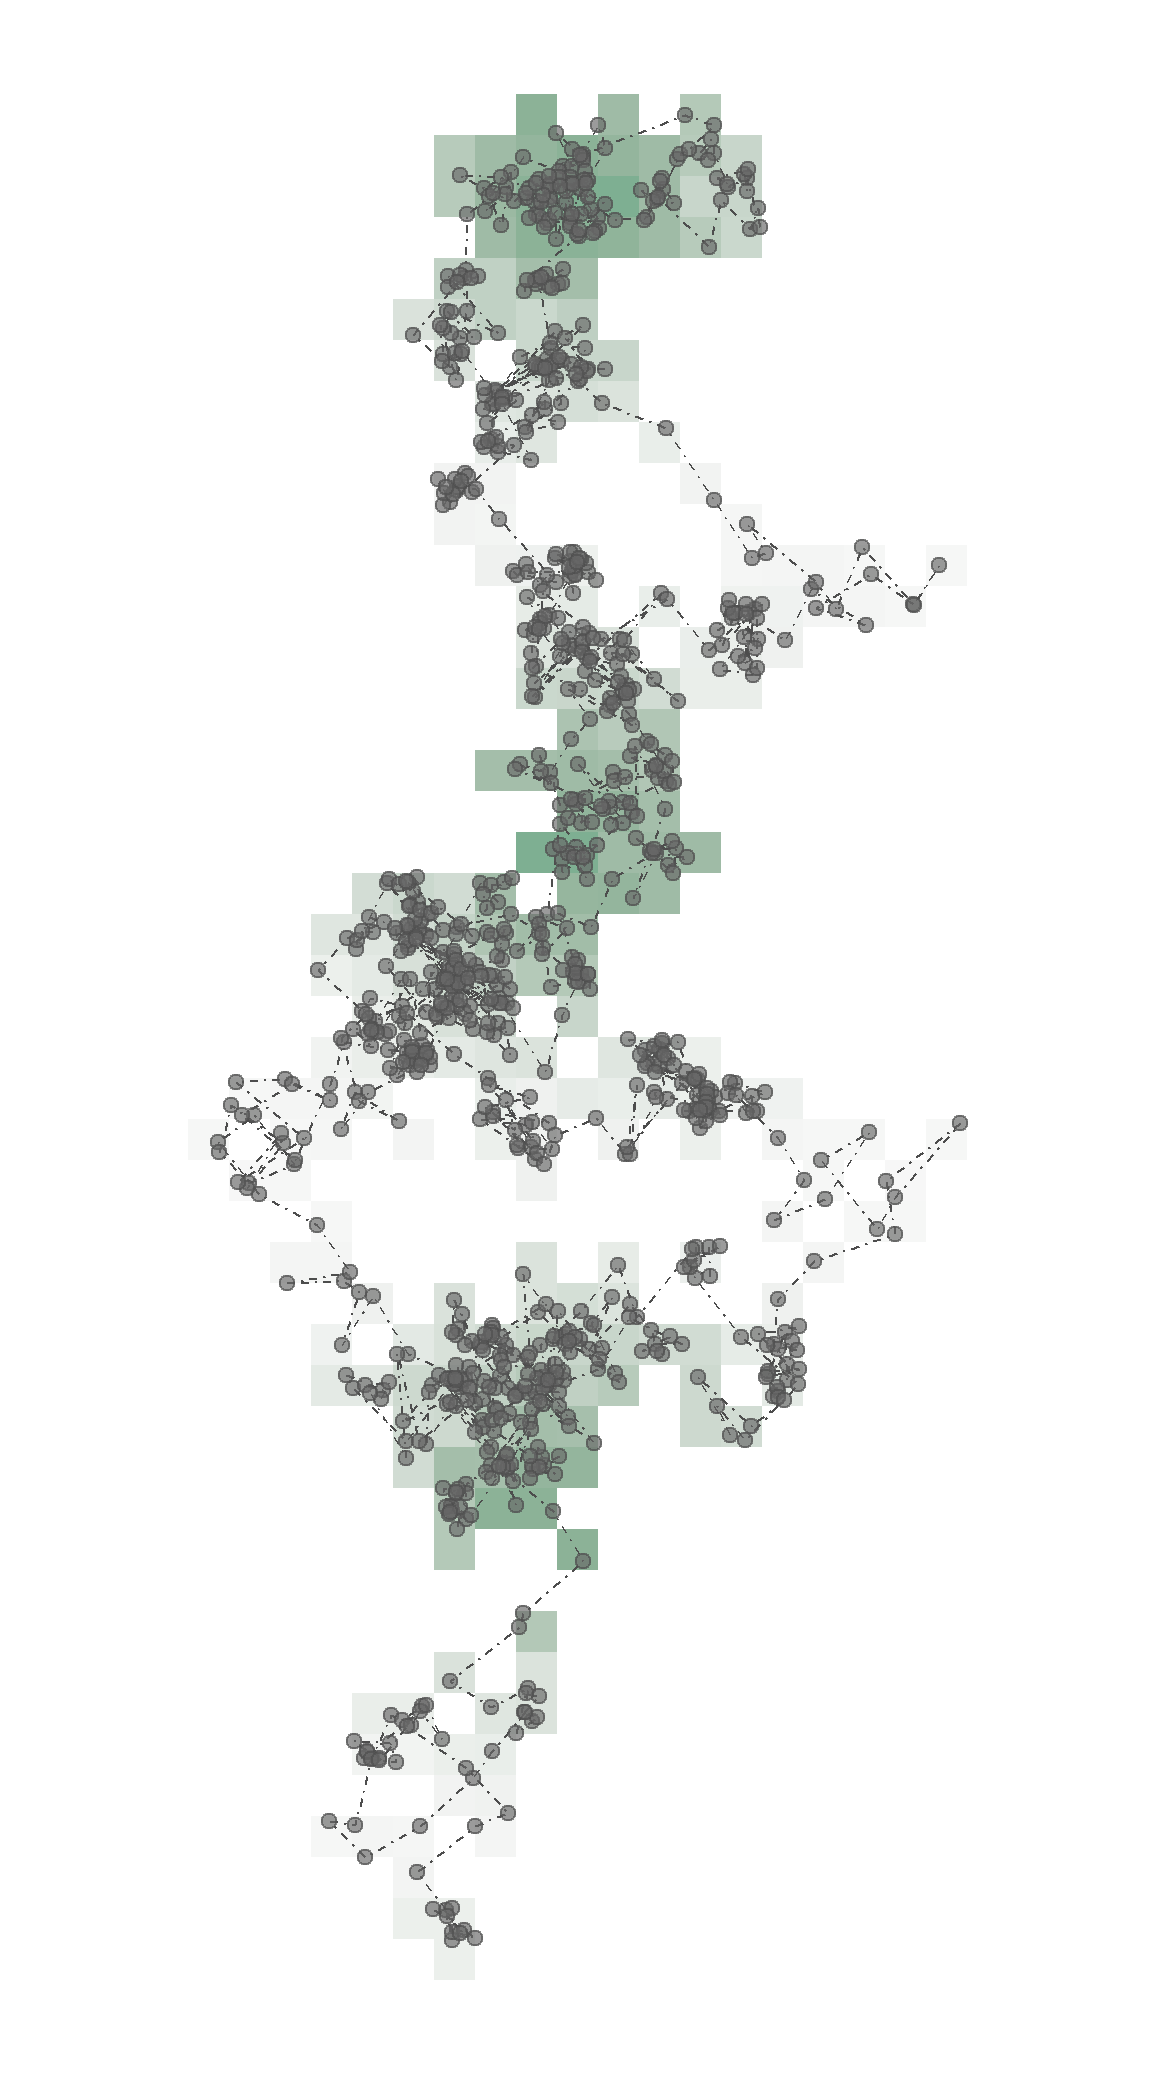
\includegraphics[width=1.0\textwidth,
          align=h,
          smash=br,
          hsmash=r,
          hshift=0.5\textwidth,
          % vshift=1cm,     % adjust the vertical position
          % hshift=-1.5cm
          ]{figures/cover_2.png}
        {
          \begin{flushleft}
            \color{SteelBlue4}{\fontsize{60}{50} \bfseries\sffamily{ANIMAL\\MOVEMENT\\STRATEGIES}\par}\par
          \end{flushleft}
        }
        % \makebox[0pt][h]{%
          % \raisebox{-\totalheight}[0pt][0pt]{%
        
          % }
        % }%
        \vspace{81mm}

        \sffamily\huge{PRATIK RAJAN GUPTE}

        \vfill

        % \includegraphics[width=6cm]{gfx/TFZsuperellipse_bw} \\ \medskip

        % \mySubtitle \\ \medskip
        %\myDegree \\
        %\myDepartment \\
        %\myFaculty \\
        %\myUni \\ \bigskip

        % \myTime\ -- \myVersion

        \vfill

    % \end{center}
  \end{addmargin}
\end{titlepage}

\nopagecolor

\thispagestyle{empty}

\hfill

\vfill

\noindent {\scshape{COLOPHON}}

\noindent The research presented in this thesis was carried out at the Department for Theoretical Research in Evolutionary Life Sciences (TRES), at the Groningen Institute for Evolutionary Life Sciences (GELIFES), at the University of Groningen's Faculty of Science and Engineering (FSE).
This research was made possible by an \emph{Adaptive Life} grant from GELIFES; part of the work in this thesis was funded by the European Research Council (ERC Advanced Grant No. 789240).
Support for this research was provided primarily by the University of Groningen; other institutions whose support made parts of this work possible are acknowledged within.
The production of this thesis was partly funded by GELIFES, the FSE, and the University of Groningen.

\medskip

\noindent This document was typeset using the \emph{classicthesis} \LaTeX~style, developed by Andr\'e Miede and Ivo Pletikosić.
% This style was inspired by Robert Bringhurst's seminal book on typography \emph{The Elements of Typographic Style}.
The text is mostly set in \emph{Timepos Text} from the New Zealand-based Klim Type Foundry, with some headings in \emph{Plex Serif} from the Dutch type foundry Bold Monday. Friedrich Althausen's \emph{Vollkorn} is used for chapter breaks.

\bigskip

\noindent\finalVersionString

\noindent\myName. \textit{\myTitle.}% \mySubtitle, %\myDegree,
\\
\noindent \textcopyright\ \today

%*******************************************************
% RUG defined Titlepage
%*******************************************************
\thispagestyle{empty}
\begin{titlepage}
    \thispagestyle{empty}
    %\pdfbookmark[1]{\myTitle}{titlepage}
    % if you want the titlepage to be centered, uncomment and fine-tune the line below (KOMA classes environment)
    \begin{addmargin}[-1cm]{-3cm}
    \begin{center}
        % \linespread{1.5}
        % \large

        \hfill
        \begin{figure*}
            
\includegraphics[width=7.38cm,height=2.03cm]{figures/rug_logo.eps}
        \end{figure*}

        \vspace{12mm}

        {
           {\fontsize{30}{30} \bfseries{Animal Movement\\Strategies}\par}\par
        }

        \vspace{21mm}

        {
           {\fontsize{15}{15} \bfseries{PhD thesis}\par}\par
        }

        \vspace{12mm}

        {\fontsize{14}{15}
            {to obtain the degree of PhD at the\\
            University of Groningen\\
            on the authority of the\\
            Rector Magnificus Prof. C. Wijmenga\\
            and in accordance with\\
            the decision by the College of Deans.}

            \vspace{3mm}

            This thesis will be defended in public on

            \vspace{3mm}

            19 August 2022 at 11:00 hours

            \vspace{12mm}

            by

            \vspace{12mm}

            \textbf{Pratik Rajan Gupte}

            \vspace{3mm}

            born on 22 September 1993\\
            in Hyderabad, India
        }
        % \vfill

        % {
        %    \myfont \color{Maroon}{\fontsize{70}{50} \bfseries\scshape{Animal Movement Strategies}\par}\par
        % }
        % % \myTitle

        % \bigskip

        % \bfseries\huge{\myName}

        % \vfill

        % % \includegraphics[width=6cm]{gfx/TFZsuperellipse_bw} \\ \medskip

        % % \mySubtitle \\ \medskip
        % %\myDegree \\
        % %\myDepartment \\
        % %\myFaculty \\
        % %\myUni \\ \bigskip

        % % \myTime\ -- \myVersion

        % \vfill

    \end{center}

    \pagebreak
    \thispagestyle{empty}

    \textbf{Supervisors}
    \begin{description}
        \item Prof. Dr. Franz J. Weissing
    \end{description}

    \vspace{6mm}

    \textbf{Co-supervisor}
    \begin{description}
        \item Whomever
    \end{description}

    \vspace{6mm}

    \textbf{Assessment committee}
    \begin{description}
        \item Whomever
        \item Whomever
        \item Whomever
    \end{description}

  \end{addmargin}

\end{titlepage}


    %\pdfbookmark[1]{\myTitle}{titlepage}
    % if you want the titlepage to be centered, uncomment and fine-tune the line below (KOMA classes environment)
    


% \cleardoublepage %*******************************************************
% Propositions
%*******************************************************
%\renewcommand{\abstractname}{Abstract}
\pdfbookmark[1]{Propositions}{Propositions}
% \addcontentsline{toc}{chapter}{\tocEntry{Abstract}}
\begingroup
% \let\clearpage\relax
% \let\cleardoublepage\relax
% \let\cleardoublepage\relax

\chapter*{Propositions}

\begin{onehalfspace}
    
    \begin{enumerate}
        \item \textit{What are birds if not dinosaurs persevering.\\--- Twitter, paraphrasing WandaVision}
        \item Animal movement ecology needs to adopt best-practices from other big-data disciplines.\\ --- \textit{Chapter 1}.
        \item Animals' movement decisions incorporate not only what they can see, but what they think other individuals can see.\\ --- \textit{Chapter 2}.
        \item Mechanistic, individual-based simulation modelling of movement decisions opens the door to the evolutionary ecology of animal movement. \\ --- \textit{Chapter 3}.
        \item Statistical tools in movement ecology are sensitive to the scale and mechanisms of individual variation.\\ ---\textit{Chapter 4}.
        \item Rapid evolution in movement strategies can drastically reshape the structure of animal societies.\\ --- \textit{Chapter 5}.
        \item \textit{Sometimes it's better to light a flamethrower than curse the darkness.\\--- Terry Pratchet}
    \end{enumerate}

\end{onehalfspace}

\endgroup

\vfill

\clearpage

% \clearpage%*******************************************************
% Dedication
%*******************************************************
\thispagestyle{empty}
\phantomsection
\pdfbookmark[1]{Dedication}{Dedication}

\vspace*{3cm}

\begin{center}
    \large\emph{What can be achieved by not listening to supervisors}
    
\end{center}
% % \clearpage\pagestyle{empty}

\hfill

\vfill


\pdfbookmark[0]{Colophon}{colophon}
\section*{Colophon}
This document was typeset based on \emph{classicthesis}, developed by Andr\'e Miede and Ivo Pletikosić.
The style was inspired by Robert Bringhurst's seminal book on typography ``\emph{The Elements of Typographic Style}''.
Inspired by Wouter Vahl's PhD thesis ``\emph{Interference Competition in Foraging Waders}'', Matthew Carter's Charter is used for the main text; Vernon Adams' Oswald is used for headings.
The cover design is inspired by the colours of the Japanese edition of Theodore M. Porter's ``\emph{Trust the Numbers}''.

\bigskip

\noindent\finalVersionString

%Hermann Zapf's \emph{Palatino} and \emph{Euler} type faces (Type~1 PostScript fonts \emph{URW
%Palladio L} and \emph{FPL}) are used. The ``typewriter'' text is typeset in \emph{Bera Mono},
%originally developed by Bitstream, Inc. as ``Bitstream Vera''. (Type~1 PostScript fonts were made
%available by Malte Rosenau and
%Ulrich Dirr.)

%\paragraph{note:} The custom size of the textblock was calculated
%using the directions given by Mr. Bringhurst (pages 26--29 and
%175/176). 10~pt Palatino needs  133.21~pt for the string
%``abcdefghijklmnopqrstuvwxyz''. This yields a good line length between
%24--26~pc (288--312~pt). Using a ``\emph{double square textblock}''
%with a 1:2 ratio this results in a textblock of 312:624~pt (which
%includes the headline in this design). A good alternative would be the
%``\emph{golden section textblock}'' with a ratio of 1:1.62, here
%312:505.44~pt. For comparison, \texttt{DIV9} of the \texttt{typearea}
%package results in a line length of 389~pt (32.4~pc), which is by far
%too long. However, this information will only be of interest for
%hardcore pseudo-typographers like me.%
%
%To make your own calculations, use the following commands and look up
%the corresponding lengths in the book:
%\begin{verbatim}
%    \settowidth{\abcd}{abcdefghijklmnopqrstuvwxyz}
%    \the\abcd\ % prints the value of the length
%\end{verbatim}
%Please see the file \texttt{classicthesis.sty} for some precalculated
%values for Palatino and Minion.
%
%    \settowidth{\abcd}{abcdefghijklmnopqrstuvwxyz}
%    \the\abcd\ % prints the value of the length


\cleardoublepage % Table of Contents
%*******************************************************
\begingroup
\raggedright
% \pagestyle{scrheadings}
\thispagestyle{empty}
\phantomsection
\pdfbookmark[1]{\contentsname}{tableofcontents}
\setcounter{tocdepth}{0} % <-- 2 includes up to subsections in the ToC
\setcounter{secnumdepth}{2} % <-- 3 numbers up to subsubsections
\manualmark
\markboth{\spacedlowsmallcaps{\contentsname}}{\spacedlowsmallcaps{\contentsname}}
\begin{onehalfspace}

    \raggedright
    \tableofcontents

    \automark[section]{chapter}
    % \renewcommand{\chaptermark}[1]{\markboth{\spacedlowsmallcaps{#1}}{\spacedlowsmallcaps{#1}}}
    % \renewcommand{\sectionmark}[1]{\markright{\textsc{\thesection}\enspace\spacedlowsmallcaps{#1}}}
\end{onehalfspace}

\endgroup
\cleardoublepage

% \tableofcontents

\frontmatter
\cleardoublepage %*******************************************************
% Abstract
%*******************************************************
%\renewcommand{\abstractname}{Abstract}
\pdfbookmark[1]{Abstract}{Abstract}
% \addcontentsline{toc}{chapter}{\tocEntry{Abstract}}
\begingroup
% \let\clearpage\relax
% \let\cleardoublepage\relax
% \let\cleardoublepage\relax

\chapter*{Abstract}

% \begin{center}
%     \emph{What are birds, if not dinosaurs persevering?}\\
%     \medskip
%     -- \small{Paraphrased from \textit{WandaVision}, 2021.}
% \end{center}

% Competition typically takes place in a spatial context, but eco-evolutionary models rarely address the joint evolution of movement and competition strategies. 
% Here we investigate a spatially explicit forager-kleptoparasite model where consumers can either forage on a heterogeneous resource landscape, or steal resource items from conspecifics (kleptoparasitism). 
% We consider three scenarios: (1) foragers without kleptoparasites; (2) consumers specializing as foragers or as kleptoparasites; and (3) consumers that can switch between foraging and kleptoparasitism depending on local conditions.
% We model movement strategies as individual-specific combinations of preferences for environmental cues, similar to step-selection coefficients.
% By means of mechanistic, individual-based simulations, we study the joint evolution of movement and competition strategies, and we investigate the implications on the resource landscape and the distribution of consumers over this landscape.
% Movement and competition strategies evolve rapidly and consistently across all scenarios, with marked differences among scenarios, leading to differences in resource exploitation patterns.
% % The evolved movement and resource exploitation patterns differ considerably across the three scenarios.
% In scenario 1, foragers evolve considerable individual variation in movement strategies, while in scenario 2, movement strategy is tightly correlated with competition strategy, with a swift divergence between foragers and kleptoparasites.
% When individuals' competition strategy is conditional on local cues, movement strategies converge to facilitate kleptoparasitism, and individual consistency in competition strategy also emerges.
% Across scenarios, the distribution of consumers over resources differs substantially from `ideal free' predictions. 
% This is related to the intrinsic difficulty of moving effectively on a depleted resource landscape with few reliable cues for movement.
% Our study emphasises the advantages of a mechanistic approach when studying competition in a spatial context, and suggests how evolutionary modelling can be integrated with current work in animal movement ecology.

% \begin{center}
% % \url{https://plg.uwaterloo.ca/~migod/research/beckOOPSLA.html}
% \end{center}

% \vfill

% \begin{otherlanguage}{ngerman}
% \pdfbookmark[1]{Zusammenfassung}{Zusammenfassung}
% \chapter*{Zusammenfassung}
% Kurze Zusammenfassung des Inhaltes in deutscher Sprache\dots
% \end{otherlanguage}

\endgroup

\vfill

\clearpage


\pagestyle{scrheadings}
\pagenumbering{arabic}
% \setcounter{page}{1}

\mainmatter

%********************************************************************
% Mainmatter
% *******************************************************

% use \clearpage here to avoid problems with pdfbookmark
\clearpage

\cleardoublepage 
\phantomsection
\addtocontents{toc}{\protect\vspace{\beforebibskip}}%
% \addcontentsline{toc}{chapter}{\tocEntry{\color{black}\itshape{General Introduction: The Current Frontiers of Animal Movement Ecology}}}%
\chapter{General Introduction: The Current Frontiers of Animal Movement Ecology}\label{ch:introduction}
\chaptermark{General Introduction}

{{Pratik R. Gupte}}

% \begin{center}
%     \emph{Coming back to where you started is not the same as never leaving.}\\
%     \medskip
%     -- \small{Terry Pratchett}
% \end{center}

% Movement is a fascinating phenomenon.
% It integrates a deep, implicit \textit{feel} for the fundamental organisation of the universe, with surprising agency: that things, colloquially speaking, need not be the same, or different.
% All animals move, whether actively or passively, at some stage of their lives.
% As humans, we have projected our own motivations on to animals around us, and arrived at a relatively good understanding of why animals move, i.e., the ecological drivers of animal movement.
% In this, we have the advantage of not being too far from our own past, before we had quite successfully insulated ourselves from the effects of such drivers.
% This allows us to take the perspective of other animals when looking at a landscape; essentially, to mentally \textit{model} movement decisions across it.

% {\color{red} WORK IN PROGRESS}

To be completed.

\vfill

\clearpage


\cleardoublepage 
\ctparttext{Some text here.\\ \centering\barfont{-.-}}
\part{Leveraging New Methods to Study Animal Movement and Spatial Ecology}
\label{part:eco}

\cleardoublepage % \begin{refsection}
%************************************************
\chapter{Pre-processing High Throughput Animal Tracking Data}\label{ch:preprocessing}
\chaptermark{Pre-processing Animal Tracking Data}
%************************************************
% 
{\noindent \textbf{Pratik R. Gupte}, Christine E. Beardsworth\textsuperscript{1}, Orr Spiegel\textsuperscript{2}, Emmanuel Lourie\textsuperscript{3}, Sivan Toledo\textsuperscript{2}, Ran Nathan\textsuperscript{3}, and Allert Bijleveld\textsuperscript{1}}

\graffito{
	{\color{Maroon}\normalsize\headerfont{Co-author Affiliations}}

    \medskip

    
    \textsuperscript{1} Netherlands Inst. for Sea Research, The Netherlands.
    
    \medskip
    
    \textsuperscript{2} Tel Aviv University, Israel.
    
    \medskip

    \textsuperscript{3} The Hebrew University of Jerusalem, Israel.

    \medskip

    {\color{Maroon}\normalsize\headerfont{Funding}}

    \medskip

    Dutch Research Council (NWO)

    \medskip

    Israel Science Foundation

    \medskip

    Minerva Foundation    
}

\section*{Abstract}
{
    % \small
    	
    Modern, high-throughput animal tracking increasingly yields `big data' at very fine temporal scales, and 
    % At these scales, location error can exceed the animal's step size, leading to mis-estimation of behaviours inferred from movement. 
    `cleaning' the data to reduce location errors is one of the main ways to deal with position uncertainty. 
    Though data cleaning is widely recommended, inclusive, uniform guidance on this crucial step, and on how to organise the cleaning of massive datasets, is relatively scarce.
    A pipeline for cleaning massive high-throughput datasets must balance ease of use and computationally efficiency, in which location errors are rejected while preserving valid animal movements. 
    % Another useful feature of a pre-processing pipeline is efficiently segmenting and clustering location data for statistical methods, while also being scalable to large datasets and robust to imperfect sampling. 
    Manual methods being prohibitively time consuming, and to boost reproducibility, pre-processing pipelines must be automated.
    We provide guidance on building pipelines for pre-processing high-throughput animal tracking data to prepare it for subsequent analyses. 
    We apply our proposed pipeline to simulated movement data with location errors, and also show how large volumes of cleaned data can be transformed into biologically meaningful `residence patches', for exploratory inference on animal space use. 
    We use tracking data from the Wadden Sea ATLAS system (WATLAS) to show how pre-processing improves its quality, and to verify the usefulness of the residence patch method. 
    Finally, with tracks from Egyptian fruit bats \textit{Rousettus aegyptiacus}, we demonstrate the pre-processing pipeline and residence patch method in a fully worked out example.
    To help with fast implementation of standardised methods, we developed the R package \textit{atlastools}, which we also introduce here. 
    Our pre-processing pipeline and \textit{atlastools} can be used with any high-throughput animal movement data in which the high data-volume combined with knowledge of the tracked individuals’ movement capacity can be used to reduce location errors. 
    % \textit{atlastools} is easy to use for beginners, while providing a template for further development. 
    % The common use of simple yet robust pre-processing steps promotes standardised methods in the field of movement ecology and leads to better inferences from data.

    \bigskip

    {\noindent \large{$\Delta$}} \normalfont Published in the \textit{Journal of Animal Ecology} as \citet{gupte2022d}. \citetitle{gupte2022d}.
}

\clearpage


% \newrefcontext[sorting=ynt]

\begin{center}
\emph{Spatial is special.\\
\medskip
-- \small{A common maxim in data science.}}
\end{center}

\section*{Abstract}
{
    % \small
    	
    Modern, high-throughput animal tracking increasingly yields `big data' at very fine temporal scales, and 
    % At these scales, location error can exceed the animal's step size, leading to mis-estimation of behaviours inferred from movement. 
    `cleaning' the data to reduce location errors is one of the main ways to deal with position uncertainty. 
    Though data cleaning is widely recommended, inclusive, uniform guidance on this crucial step, and on how to organise the cleaning of massive datasets, is relatively scarce.
    A pipeline for cleaning massive high-throughput datasets must balance ease of use and computationally efficiency, in which location errors are rejected while preserving valid animal movements. 
    % Another useful feature of a pre-processing pipeline is efficiently segmenting and clustering location data for statistical methods, while also being scalable to large datasets and robust to imperfect sampling. 
    Manual methods being prohibitively time consuming, and to boost reproducibility, pre-processing pipelines must be automated.
    We provide guidance on building pipelines for pre-processing high-throughput animal tracking data to prepare it for subsequent analyses. 
    We apply our proposed pipeline to simulated movement data with location errors, and also show how large volumes of cleaned data can be transformed into biologically meaningful `residence patches', for exploratory inference on animal space use. 
    We use tracking data from the Wadden Sea ATLAS system (WATLAS) to show how pre-processing improves its quality, and to verify the usefulness of the residence patch method. 
    Finally, with tracks from Egyptian fruit bats \textit{Rousettus aegyptiacus}, we demonstrate the pre-processing pipeline and residence patch method in a fully worked out example.
    To help with fast implementation of standardised methods, we developed the R package \textit{atlastools}, which we also introduce here. 
    Our pre-processing pipeline and \textit{atlastools} can be used with any high-throughput animal movement data in which the high data-volume combined with knowledge of the tracked individuals’ movement capacity can be used to reduce location errors. 
    % \textit{atlastools} is easy to use for beginners, while providing a template for further development. 
    % The common use of simple yet robust pre-processing steps promotes standardised methods in the field of movement ecology and leads to better inferences from data.
}

\newpage

\section*{Introduction}

\lettrine{A}{nimal} movement is an adaptive, integrated response to multiple drivers, including internal state, life-history traits and capacities, biotic interactions, and other environmental factors \citep{nathan2008a, holyoak2008}.
% Movement has both beneficial and detrimental consequences for individual fitness, and 
The movement ecology framework links the drivers, processes, and fitness outcomes of animal movement \citep{nathan2008a}, and remotely tracking individual animals in the wild is the methodological mainstay of movement ecology \citep{wikelski2007,nathan2008a,hussey2015,kays2015}.
A key challenge with observed tracks is to extract information on the behavioural, cognitive, social, ecological and evolutionary processes that shape animal movement.
Addressing this challenge requires investigating the relationships between movement and its drivers at the fine scales at which animals sense and respond to variation in their environment. 
Tracking data, which are observations of a continuous process (animal movement) at discrete timesteps, reveal useful information about the movement process when the tracking interval is considerably shorter than the typical duration of a movement mode \citep{nathan2008a, noonan2019, getz2008}.
This can be accomplished by wildlife tracking systems that collect position data from many individuals at high temporal and spatial resolution (i.e., high-throughput tracking) relative to the scale of the movement mode of interest \citep{getz2008}.

High-throughput tracking technologies include GPS tags \citep{strandburg-peshkin2015, papageorgiou2019, harel2016, klarevas-irby2021}, tracking radars \citep{horvitz2014}, and computer vision methods for tracking entire groups of animals from video recordings \citep{rathore2020, perez-escudero2014}. 
Furthermore, high-throughput wildlife tracking is routinely provided by terrestrial reverse-GPS systems such as ATLAS \citep[Advanced Tracking and Localization of Animals in real-life Systems:][]{toledo2014, weiser2016, toledo2016,toledo2020} --- see also \citep{maccurdy2009, maccurdy2019} --- and underwater acoustic reverse-GPS tracking of aquatic animals \citep{baktoft2019, baktoft2017, jung2015, aspillaga2021, aspillaga2021a}.
Finally, low resolution tracking over a long duration may also capture important aspects of animal behaviour at certain time-scales \citep[e.g. migration, long-range dispersal;][]{getz2008}, thereby being `relatively' high-throughput.

Although high-throughput tracking provides a massive amount of data on the path of a tracked animal, these data present a challenge to ecologists.
When tracking animals at a high temporal resolution, the location error of each position may approach or exceed the true movement distance of the animal, compared to low-resolution tracking with the same measurement error.
This leads to an over-estimation of the true distance moved by an animal between two discrete time-points, leading to unreliable behavioural metrics ultimately derived from movement distance, such as speed and tortuosity \citep[see][]{ranacher2016, noonan2019, hurford2009, calenge2009}.
Additionally, the location error around a position introduces uncertainty when studying the relationship between animal movements and either fixed landscape features (e.g. roads), or mobile elements (e.g. other tracked individuals), as well as confounding estimates of habitat selection.

Users have two main options to improve data quality, \textit{(i)} making inferences after modelling the system-specific location error using a continuous time movement model \citep{fleming2014, fleming2020, jonsen2003, jonsen2005, johnson2008, patterson2008, aspillaga2021}, or \textit{(ii)} pre-processing data to clean it of positions with large location errors \citep{bjorneraas2010}.
The first approach may be limited by the animal movement models that can be fitted to the data \citep{fleming2014, noonan2019, fleming2020}, may result in unreasonable computation times, or may be entirely beyond the computational capacity of common hardware, leading users to prefer data cleaning instead.
Data cleaning reveals another challenge of high-throughput tracking: the large number of observations make it difficult for researchers to visually examine each animal's track for errors \citep{weiser2016, toledo2020}.
With manual identification and removal of errors from individual tracks prohibitively time consuming, data cleaning can benefit from automation based on a protocol.

Pre-processing of movement data --- defined as the set of data management steps executed prior to data analysis --- must reliably discard large location errors, also called outliers, from tracks (analogous to reducing false positives) while avoiding the overzealous rejection of valid animal movements (analogous to reducing false negatives).
How well researchers balance these imperatives has consequences for downstream analyses \citep{stine2001}.
For instance, small-scale resource selection functions can easily infer spurious preference and avoidance effects when there is uncertainty about an animal's true position \citep{visscher2006}.
Ecologists recognise that tracking data are imperfect observations of the underlying movement process, yet they implicitly consider cleaned data equivalent to the ground-truth.
This assumption is reflected in popular statistical methods in movement ecology such as Hidden Markov Models (HMMs) \citep{langrock2012}, stationary-phase identification methods \citep{patin2020a}, or step-selection functions (SSFs) \citep{barnett2008, signer2017, avgar2016}, which expect minimal location errors relative to real animal movement (i.e., a high signal-to-noise ratio).
This makes the reproducible, standardised removal of location errors crucial to any animal tracking study.
While gross errors are often removed by positioning-system algorithms in both GPS and reverse-GPS setups, `reasonable' errors often remain to confront end users \citep{fischler1981, weiser2016, ranacher2016}.
Further, as high-throughput tracking is deployed in more regions and for more species, standardised pre-processing steps should be general enough to tackle animal movement data recovered from a range of environments, so as to enable sound comparisons across species and ecosystems.

Despite the importance and ubiquity of reducing location errors in tracking data, movement ecologists lack formal guidance on this crucial step.
Pre-processing protocols are not often reported in the literature, or may not be easily tractable for mainstream computing hardware and software.
Some tracking data, such as GPS, are autonomously pre-processed without user access to the raw data \citep[using error estimates and Kalman smooths;][and substantial location errors may yet persist]{kaplan2005}.
However, filtering out positions using estimates of location error alone may not be sufficient to exclude outliers which represent unrealistic movement but have low error measures \citep{weiser2016, ranacher2016}.
When tracking systems do make their raw data available to researchers, this can enable users to better control the data pre-processing stage, and to substantially improve data quality while ensuring that cleaning does not itself lead to unrealistic movement tracks \citep[e.g. Kalman smooths which distort tracks,][]{kaplan2005}.
This makes identifying and removing biologically implausible locations from a track an important component of recovering true animal movement \citep{bjorneraas2010}.

Even after removing unrealistic movement, a track may be comprised of positions that are randomly distributed around the true animal location \citep{noonan2019}.
The large data-volumes of high-throughput tracking allow for a neat solution: tracks can be `median smoothed' to reduce small location errors that have remained undetected \citep[e.g.][]{bijleveld2016}.
Large data volumes may also need to be thinned, for example, examining environmental covariates as predictors of prolonged residence in an area  \citep[see e.g.][]{bracis2018, aarts2008, bijleveld2016, oudman2018, harel2016} might require thinning of high-resolution movement data to match the lower spatial resolution of environmental measurements. 
Data thinning and clustering are also required to avoid non-independent observations due to strong spatio-temporal autocorrelation, or to examine the effect of sampling scale on movement metrics and resource-selection \citep{fleming2014,noonan2019}.

When dealing with datasets that contain many millions of positions, reseachers may run into computational limits when trying to apply pre-processing steps to their full dataset.
For instance, the size of working memory (RAM) limits the size of datasets that can be loaded into \textit{R}, the programming and statistical language of choice in movement ecology \citep{r2020,joo2020,joo2020a}.
Data-rich fields such as genomics inspire a possible solution: to break very large data into smaller subsets, and pass these subsets through automated computational `pipelines' \citep{schadt2010,peng2011}.
Pre-processing pipelines for animal tracking data --- the set of steps that users apply to prepare the data for a specific analysis --- come with some additional concerns: \textit{(i)} identifying which pre-processing steps are necessary, and \textit{(ii)} ensuring that these steps reproducibly operate on the data as expected, and as efficiently as possible.

While exploratory data analysis and visualisation can help determine how to pre-process the data to maximise the signal to noise ratio \citep{slingsby2016}, standardising implementations of pre-processing techniques into robust, version controlled software packages \citep[e.g. in \textit{R}, see]{wickham2015}, can increase the reliability and reproducibility of animal movement ecology \citep{haddaway2015,archmiller2020,powers2019,lewis2018}.
Overcoming hard computational constraints on speed and memory usage for very large data will often require a combination of programming strategies, such as using tools optimised for tabular data, or parallelised processing.

Here, we present guidelines for reproducibly pre-processing high-throughput animal tracking data (Fig.~\ref{preproc_fig_01}), with a focus on simple, widely generalisable steps that help improve data quality (Fig.~\ref{preproc_fig_02}).
We take two important considerations into account, that \textit{(i)} the pre-processing steps should be easily understood and reproduced, and \textit{(ii)} our implementations must be computationally efficient and reliable.
Consequently, formalising tools as functions in an \textit{R} package would improve portability and reproducibility \citep{marwick2018, wickham2015}.
Using simulated movement tracks, we demonstrate simple yet robust implementations of the pre-processing steps we recommend, conveniently wrapped into the \textit{R} package \textit{atlastools} \citep{gupte2020a}, with a discussion of features that make these steps more reproducible, and more efficient.
We also suggest one potential application of high-throughput tracking in studies of animal movement and space use, illustrated by the first-principles based synthesis of `residence patches' from clusters of spatio-temporally proximate positions \citep[\textit{sensu}][]{bijleveld2016, oudman2018, barraquand2008}.

In two fully worked out examples using our package on real tracking data, we show how to apply basic spatio-temporal and data quality filters, how to filter out unrealistic movement, and how to reduce the effect of location error with a median smooth.
In the first example, using calibration data from an ATLAS system, we show how the residence patch segmentation-clustering method can be used to accurately identify areas of prolonged residence under real field conditions.
Finally, in our second example, we use ATLAS data from Egyptian fruit bats (\textit{Rousettus aegyptiacus}) tracked in the Hula Valley, Israel, to show a fully worked out example of the pre-processing pipeline and the residence patch method.
While our approach to high-throughput tracking data, and our package of pre-processing functions was developed with reverse-GPS ATLAS systems in mind, both are broadly suitable to a wide range of high-throughput animal tracking data sources, from underwater acoustic reverse-GPS \citep{baktoft2019, baktoft2017, jung2015, aspillaga2021, aspillaga2021a}, high-resolution GPS \citep{strandburg-peshkin2015, papageorgiou2019, harel2016, klarevas-irby2021}, tracking radars \citep{horvitz2014}, and visual video tracking \citep{rathore2020, perez-escudero2014}.

% \afterpage{
    \begin{sidewaysfigure}[p]
        \centering
        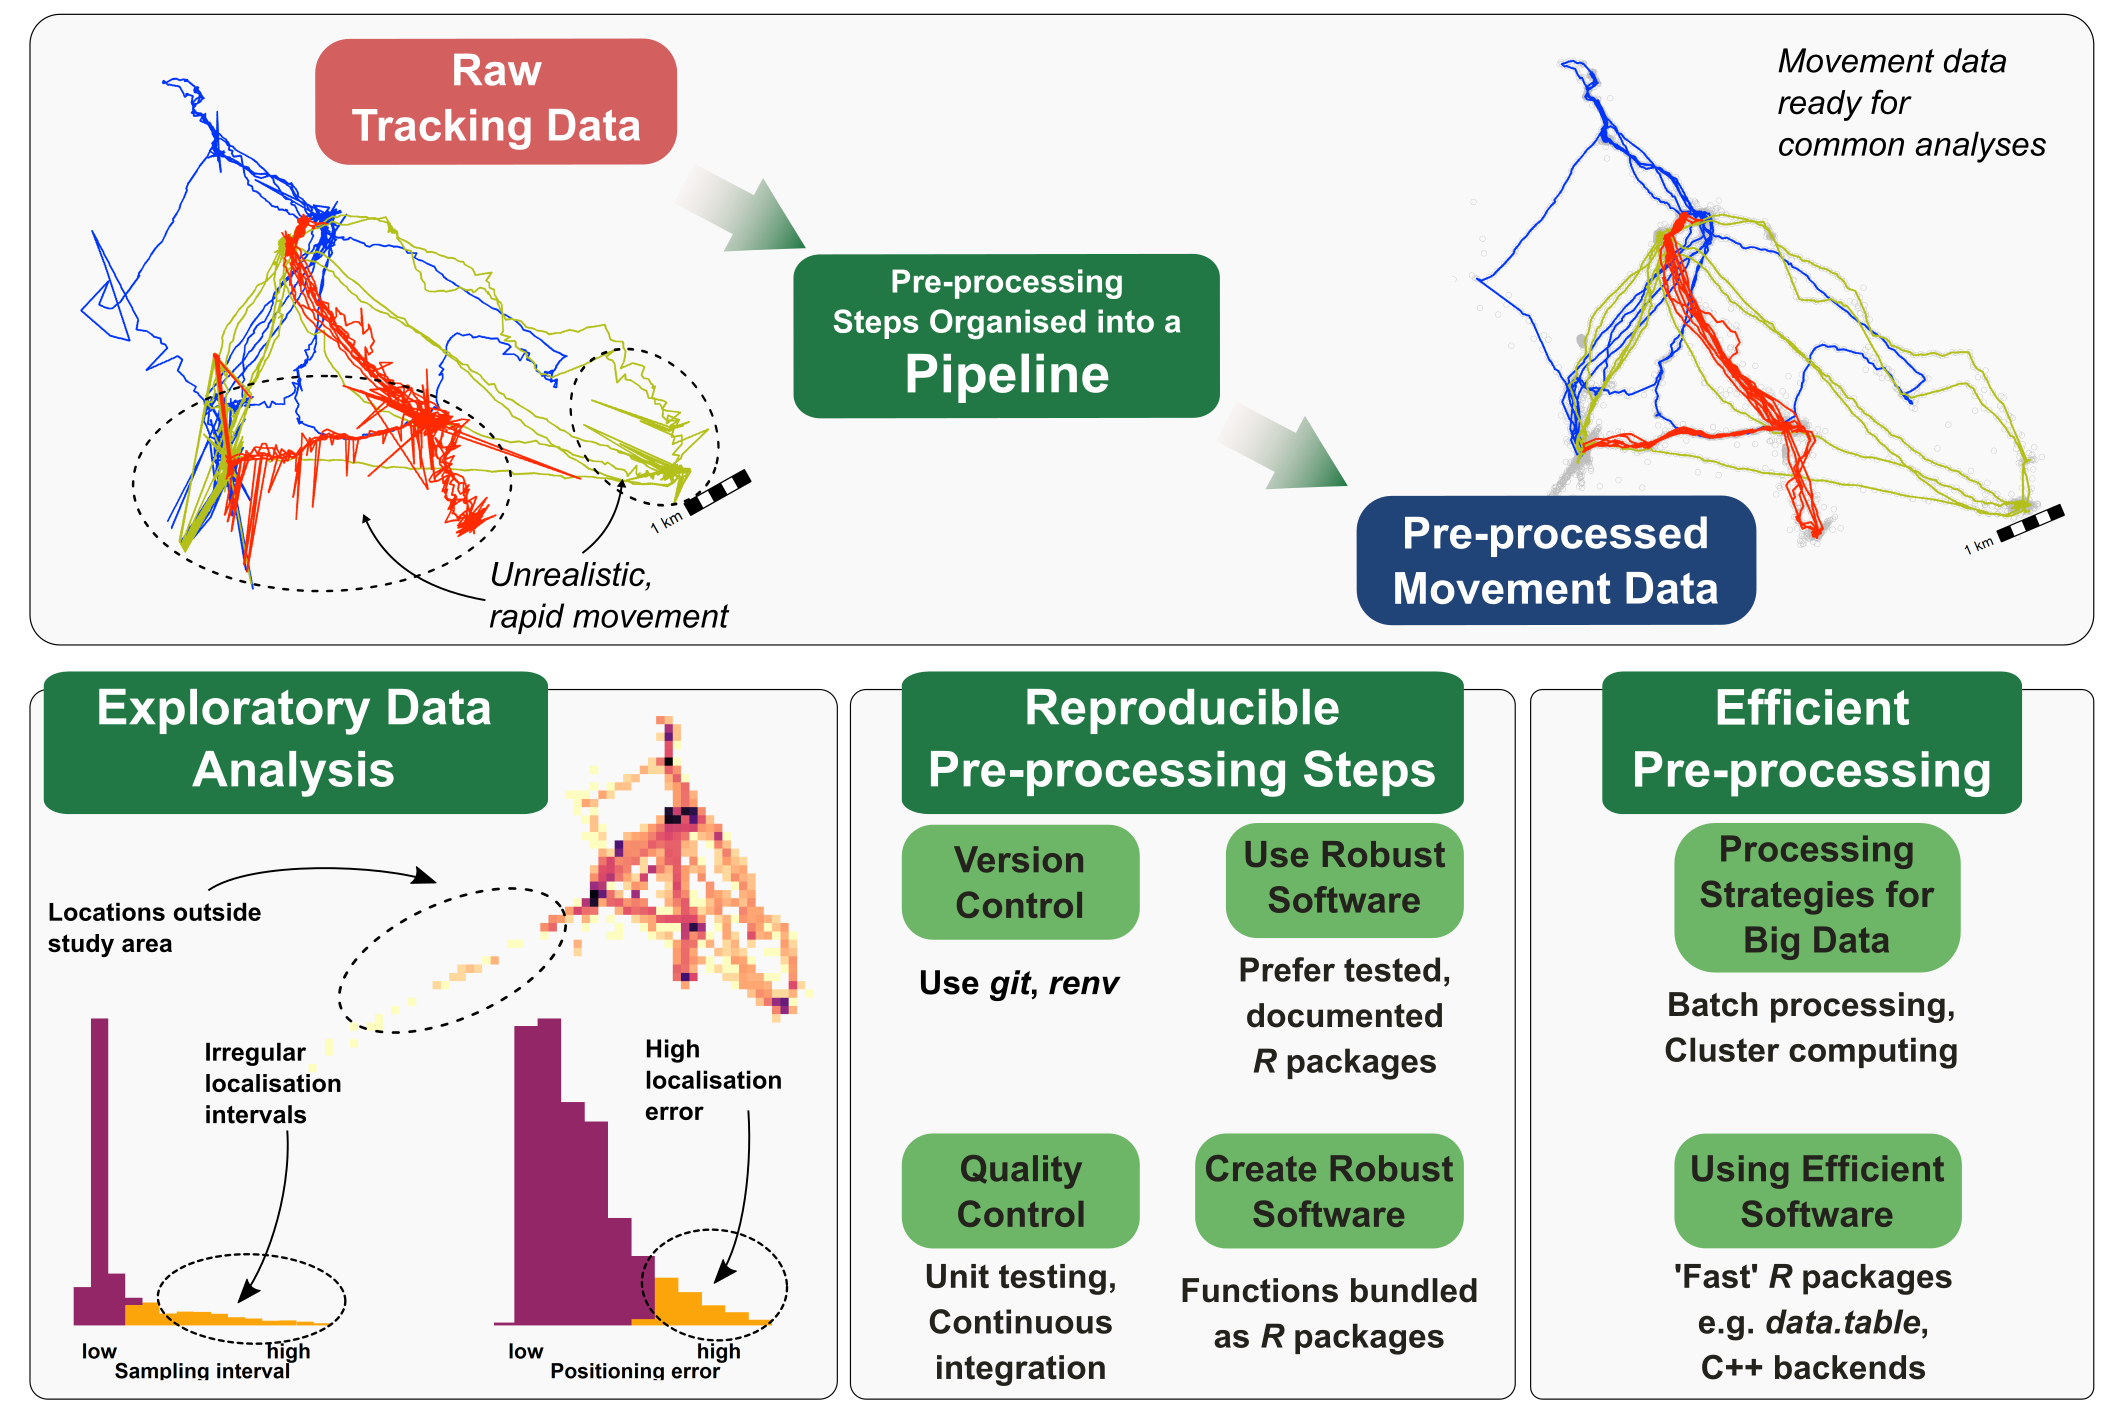
\includegraphics[width=0.7\textwidth]{figures/preprocessing/fig_01.png}
        \caption{
            \textbf{Some best-practices for pre-processing high-throughput tracking data.}
            Simple pre-processing of animal tracking data can improve the quality of animal tracking data, and the inferences that are drawn from it.
            % The organisation of pre-processing workflows into a `pipeline' --- a set of steps that users apply to prepare the data for a specific analysis --- can help make research more reproducible and reliable.
            Exploratory data analysis of representative subsets of the data can help to identify common issues with data quality, and to determine which pre-processing, steps such as filters and smooths, might be necessary (\textit{see also Fig.~\ref{preproc_fig_02}}).
            Pre-processing steps implemented as programming code can be made reproducible and shareable by following best-practices for software development: (i) tracking changes to the steps, and the software used, using version control (e.g. \textit{git}, \textit{renv}), (ii) preferring pre-existing tools, such as \textit{R} packages, which are well documented and tested, (iii) encapsulating custom-written code as functions, and bundling related functions into a package, and (iv) checking the quality of both custom-written code (e.g. by testing functions), and the overall pipeline (e.g. data visualisation).
            The efficiency of pre-processing steps can be increased by using strategies for dealing with large datasets, such as batch processing, or using a computing cluster.
            The use of existing tools optimised for large datasets, or by writing code in a `fast' language such as \textit{C++}, can also speed up the pre-processing of large datasets (see main text for examples).
            % See the \textit{Worked Out Example} on Egyptian fruit bats, as well as Supplementary Material 1, for more details on implementing pipelines.
            % Fig.~\ref{preproc_fig_02} shows an example of such a pipeline.
        }
        \label{preproc_fig_01}
    \end{sidewaysfigure}
% }

\afterpage{
    \begin{sidewaysfigure}[p]
        \centering
        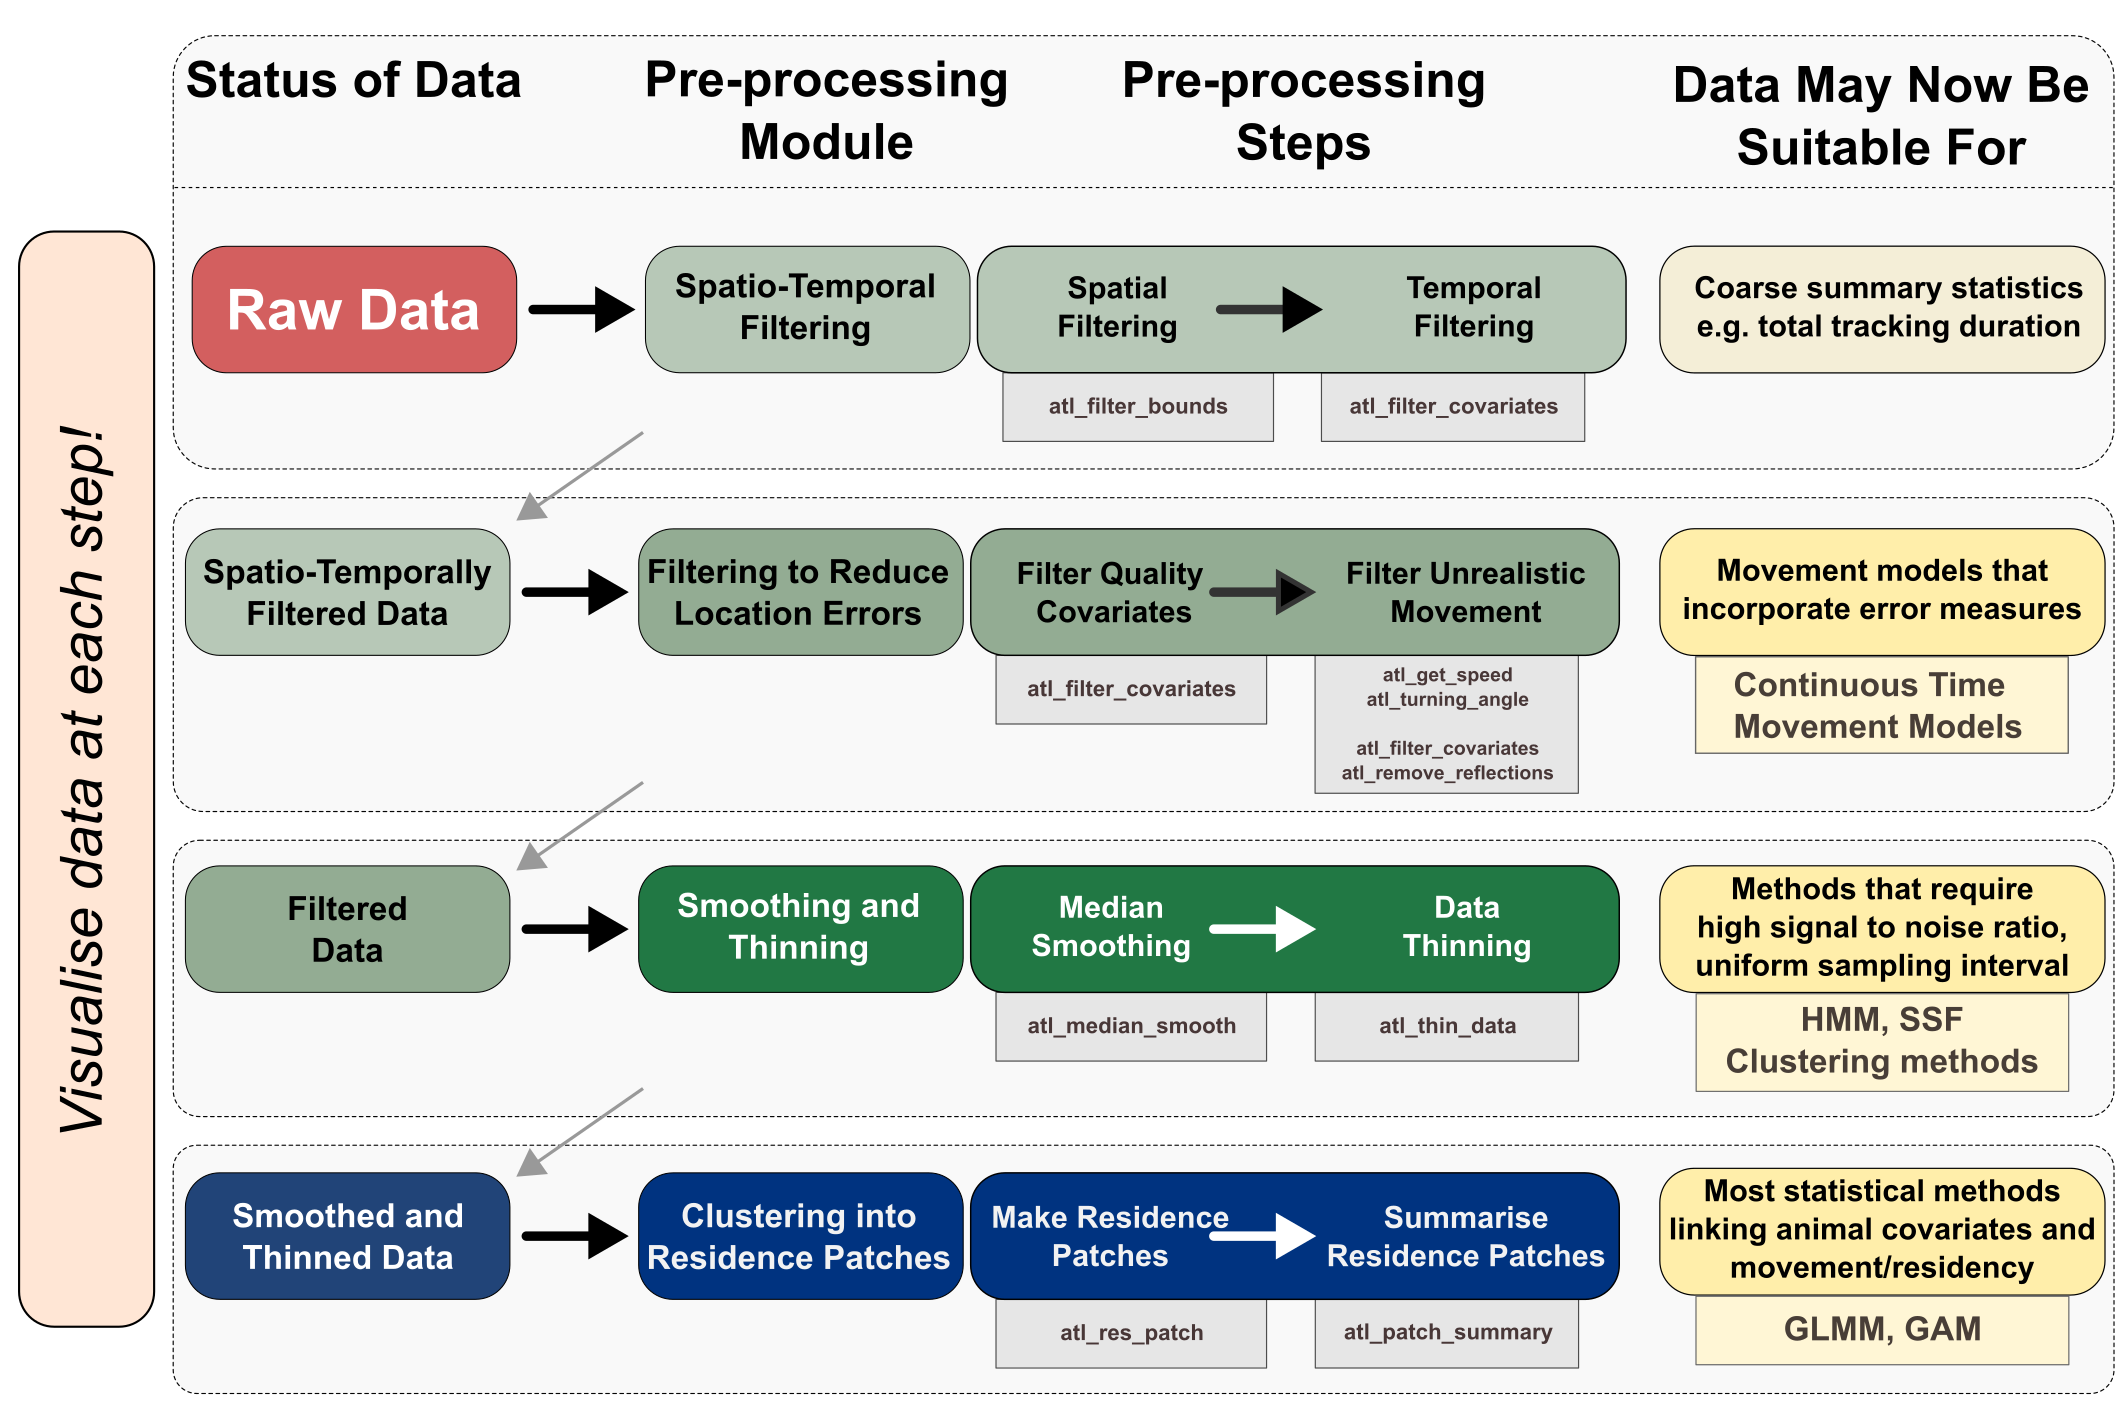
\includegraphics[width=0.7\textwidth]{figures/preprocessing/fig_02.png}
        \caption{
            \textbf{An example of a modular pipeline for pre-processing high-throughput tracking data from raw localisations to cleaned data, and optionally into residence patches.}
            Users should apply the appropriate pre-processing modules and the steps therein until the data are suitable for their intended analysis, some of which are suggested here.
            The \textit{atlastools} function that may be used to implement each pre-processing step is shown in the grey boxes underneath each step.
            Popular statistical methods are shown underneath possible analyses (yellow boxes).
            Users are strongly encouraged to visualise their data and scan it for location errors as they work through the pipeline, always asking the question, could the animal plausibly move this way?
        }
        \label{preproc_fig_02}
    \end{sidewaysfigure}
}

\section*{Best-Practices for Pre-Processing Workflows}

Exploratory data analysis should be the first step towards pre-processing movement data \citep[see Fig.~\ref{preproc_fig_01};][]{slingsby2016}.
Researchers with very large datasets of perhaps millions of rows should ideally select a representative subset of these data for exploratory data analysis, including individuals of different species, sexes, or seasonal cohorts.
Examples of exploratory data analysis include plotting heatmaps of the number of observations per unit area across the study site (Fig.~\ref{preproc_fig_01}).
Histograms of the location error estimates, plotting the linear approximations of animal paths between observations, and histograms of the sampling interval can help determine how data need to be treated so as to minimise location errors and improve computational tractability (Fig.~\ref{preproc_fig_01}).
While pre-processing steps required for datasets will differ between studies and tracking technologies, we elaborate upon candidate steps and their parameterisation in following sections (see also Fig.~\ref{preproc_fig_02}).

Following exploratory data analysis and the parameterisation of data cleaning steps, the specific implementation of these steps should be made reliable and reproducible.
Since reproducing pre-processing steps can be challenging when using only written descriptions from published articles, providing the code to implement pre-processing steps reduces ambiguity and increases reproducibility \citep{haddaway2015}.
For technically advanced users, the best-practices here are \textit{(i)} to implement pre-processing steps as `functions', \textit{(ii)} to collect related functions --- e.g. for similar kinds of data --- into a software `package', \textit{(iii)} to `test' that the functions handle input as expected, and \textit{(iv)} implement `version control' throughout, such that the process of development is documented \citep[Fig.~\ref{preproc_fig_01};][]{wickham2015,alston2020,perez-riverol2016}.

As an example, our \textit{atlastools} package incorporates these best-practices, and may be used as a reference \citep[][]{gupte2020a}.
We have written each pre-processing step as a separate function, and each of these functions is tested, usually on simulated data, but in some cases also on empirical data \citep[][see the directory \textit{tests/} in the associated Zenodo repository]{wickham2015}.
Finally, logging error messages is crucial when passing data through a pipeline, helping determine which data subsets could not be handled as expected, and why.
Users who would prefer to rely on pre-existing toolsets and methods can use \textit{R} packages that follow these best-practices, such as \textit{move} \citep{kranstauber2011}, and \textit{sftrack} \citep{boone2020}.
The large size of modern, high-throughput animal tracking data means that the computational challenge can often be \textit{the} main challenge in working with these data.
For beginning users, organising their workflows so that they process subsets of the data (such as one individual) at a time can help overcome limitations on working memory.
Animal tracking data stored in a relational database \citep[e.g. SQL databases][]{codd1970}, for example, can be broken into meaningful subsets based on individual identity and tracking season.
These smaller subsets can then be loaded into working memory, pre-processed, and saved in a separate location (see Supplementary Material 1, Section 2 for a worked out example on an SQL database).
Using existing tools optimised for tabular data, such as the \textit{R} package \textit{data.table} \citep{dowle2020}, can also speed up computation; \textit{atlastools} is built using \textit{data.table} for this reason.

More advanced users seeking substantial speed gains might wish to look into parallel-processing, and process each subset of the data independently of the full dataset, for example by using a computing cluster \citep[see also][for an alternative]{zjdai2021}.
Finally, another advanced method, used by popular packages such as \textit{move} \citep{kranstauber2011} and \textit{recurse} \citep{bracis2018}, is to write one's own methods in a `fast' low-level language, such as \textit{C++}, and link these to \textit{R} \citep[][]{eddelbuettel2013}; see also \textit{adehabitatLT}, which is written partially in \textit{C} \citep{calenge2006}.
Beginning practitioners can organise their workflows around these packages to benefit from the features they incorporate.

\section*{Pre-processing Steps, Usage, and Simulating Data}

\subsection*{An Overview of Pre-processing Steps and `atlastools'}

In the sections that follow, we lay out pre-processing techniques for raw high-throughput tracking data, and demonstrate working examples of these techniques, which we have collected in the \textit{R} package \textit{atlastools} (see Fig.~\ref{preproc_fig_02}).
Our package is aimed at getting `raw data' to the `analysis' stage identified by Joo et al. (2020) in their review of \textit{R} packages in movement ecology.
The package is based on \textit{data.table}, a fast implementation of data frames; thus it is compatible with a number of data structures from popular packages including \textit{move}, \textit{sftrack}, and \textit{ltraj} objects, which can be converted to data frames \citep[][]{kranstauber2011,boone2020,calenge2009}.
Our package functions are suitable for use with both regularly sampled data, as well as data with missing observations.

We cover, first, the use of simple \textit{\textbf{Spatio-Temporal Filters}} to select positions within a certain time or area.
Next, we show how users can \textit{\textbf{Reduce Location Errors}} by removing unreliable positions based on a system-specific error measure, or by the plausibility of associated movement metrics, such as speed and turning-angle \citep{seidel2018, calenge2009}.
We then show how users can tackle small-scale location errors by applying a \textit{\textbf{Median Smooth}}, and users who need uniformly sampled data, can undertake \textit{\textbf{Data Thinning}} by either aggregation or subsampling.
At this stage, the data are ready for a number of popular statistical treatments such as Hidden Markov Model-based classification \citep{michelot2016,langrock2012}.
Finally, we show how users wishing simple, efficient segmentation-clustering of points where the animal showed prolonged residence, can classify their data into `residence patches' \citep{barraquand2008, bijleveld2016} based on the movement ecology of their study species, after filtering out travelling segments (see \textit{\textbf{System-Specific Pre-Processing Tools}}).

These pre-processing techniques and package were designed with ATLAS systems in mind, motivated to meet the rapid growth of studies using this high-throughput system worldwide: in Israel \citep{toledo2014, toledo2016, toledo2020, corl2020, vilk2021}, the UK \citep{beardsworth2021a, beardsworth2021b}, and the Netherlands \citep[][]{beardsworth2022mee,bijleveld2021}. 
However, the principles and functions presented here are ready for use with other massive high-resolution data collected by GPS \citep[e.g.][]{papageorgiou2019}, reverse-GPS \citep[e.g.][]{aspillaga2021} or any other high-throughput tracking system .
Users may construct a pre-processing pipeline comprising of all the techniques we cover, or implement the modules most suitable for their data.
Users are advised to visualise their data throughout their workflow, and especially to perform thorough exploratory data analysis, to check for evident location errors or other issues \citep{slingsby2016}.


\subsection*{Simulating Data to Demonstrate Pre-Processing Steps}

To demonstrate pre-processing steps, we simulated a realistic movement track of 5,000 positions using an unbiased correlated velocity model (UCVM) implemented via the \textit{R} package \textit{smoove} \citep[][see Fig.~\ref{preproc_fig_03}.a]{gurarie2017}.
We added four kinds of error to the simulated track: (i) normally distributed small-scale offsets to the X and Y coordinates (small-scale error), (ii) normally distributed large-scale offsets to a random subset (0.5 \%) of the positions (spikes), (iii) large-scale displacement of a continuous sequence of 300 of the 5,000 positions (prolonged spikes; indices 500 -- 800), and (iv) we removed 10\% of the canonical track to simulate missing data (see Fig.~\ref{preproc_fig_03}.a).
To demonstrate the residence patch method, we obtained data, in the form of 1,000 positions, from a mechanistic, individual-based simulation model, in which agents move using simple decision making rules, and can find high-productivity patches using only ephemeral cues, such as the density of prey-items and other competitors \citep{gupte2021a, netz2022a}.
The emergent, complex track structure is analogous to the foraging movements of animals, and provides a suitable challenge for the residence patch method and helps to demonstrate its generality.

\section*{Spatio-Temporal Filtering}

\subsection*{Spatial Filtering Using Bounding Boxes and Polygons}

First, users should exclude positions outside the spatial bounds of a study area by comparing position coordinates with the range of acceptable coordinates (the bounding box), and removing positions outside them (Fig.~\ref{preproc_fig_03}.a). 
A bounding box filter does not require a geospatial representation such as a shapefile, and can help remove unreliable data from a tracking system that is less accurate beyond a certain range \citep[][]{beardsworth2022mee}.
In some special cases, users may wish to remove positions \textit{inside} a bounding box, either because movement behaviour within an area is not the focus of a study, or because positions recorded within an area are known to be erroneous.
An example of the former is studies of transit behaviour between features which can be approximated by their bounding boxes. 
Instances of the latter are likely to be system specific, but are known from ATLAS systems. 
Bounding boxes are typically rectangular, and users seeking to filter for other geometries, such as a circular or irregularly-shaped study area, need a geometric intersection between their data and a spatial representation of the area of interest (e.g. shapefile, geopackage, or \textit{sf}-object in \textit{R}).
The \textit{atlastools} function \textit{atl\_filter\_bounds} implements both bounding box and explicit spatial filters, and accepts X and Y coordinate ranges, an \textit{sf}-polygon or multi-polygon object \citep{pebesma2018}, or any combination of the three to filter the data.
When both coordinate ranges and a polygon are provided, the data is first filtered by the ranges and then the polygon.
The boolean function argument \textit{remove\_inside} determines whether positions inside the bounds are retained (\textit{FALSE}) or removed (\textit{TRUE}).

% \begin{lst{\color{red} Listing}}[float,floatplacement=h!,language=R, style=customR, caption = {
%     The \textit{atl\_filter\_bounds} function filters on an area defined by coordinate ranges, a polygon, or all three; it can remove positions outside (\textit{remove\_inside = FALSE}), or within the area (\textit{remove\_inside = TRUE}).
%     The arguments \textit{x} and \textit{y} determine the X and Y coordinate columns, \textit{x\_range} and \textit{y\_range} are the filter bounds in a coordinate reference system in metres, and the data can be filtered by an \textit{sf-(MULTI)POLYGON}, which can be passed using the \textit{sf\_polygon} argument. 
%     The output is a \textit{data.table}, which must be saved as an object (here, \textit{filtered\_data}).}]
% filtered_data <- atl_filter_bounds(
%                         data = data,
%                         x = "X", y = "Y",
%                         x_range = c(x_min, x_max),
%                         y_range = c(y_min, y_max),
%                         sf_polygon = your_polygon,
%                         remove_inside = FALSE
%                     )
% \end{lst{\color{red} Listing}}

\begin{figure}[ht!]
    \centering
    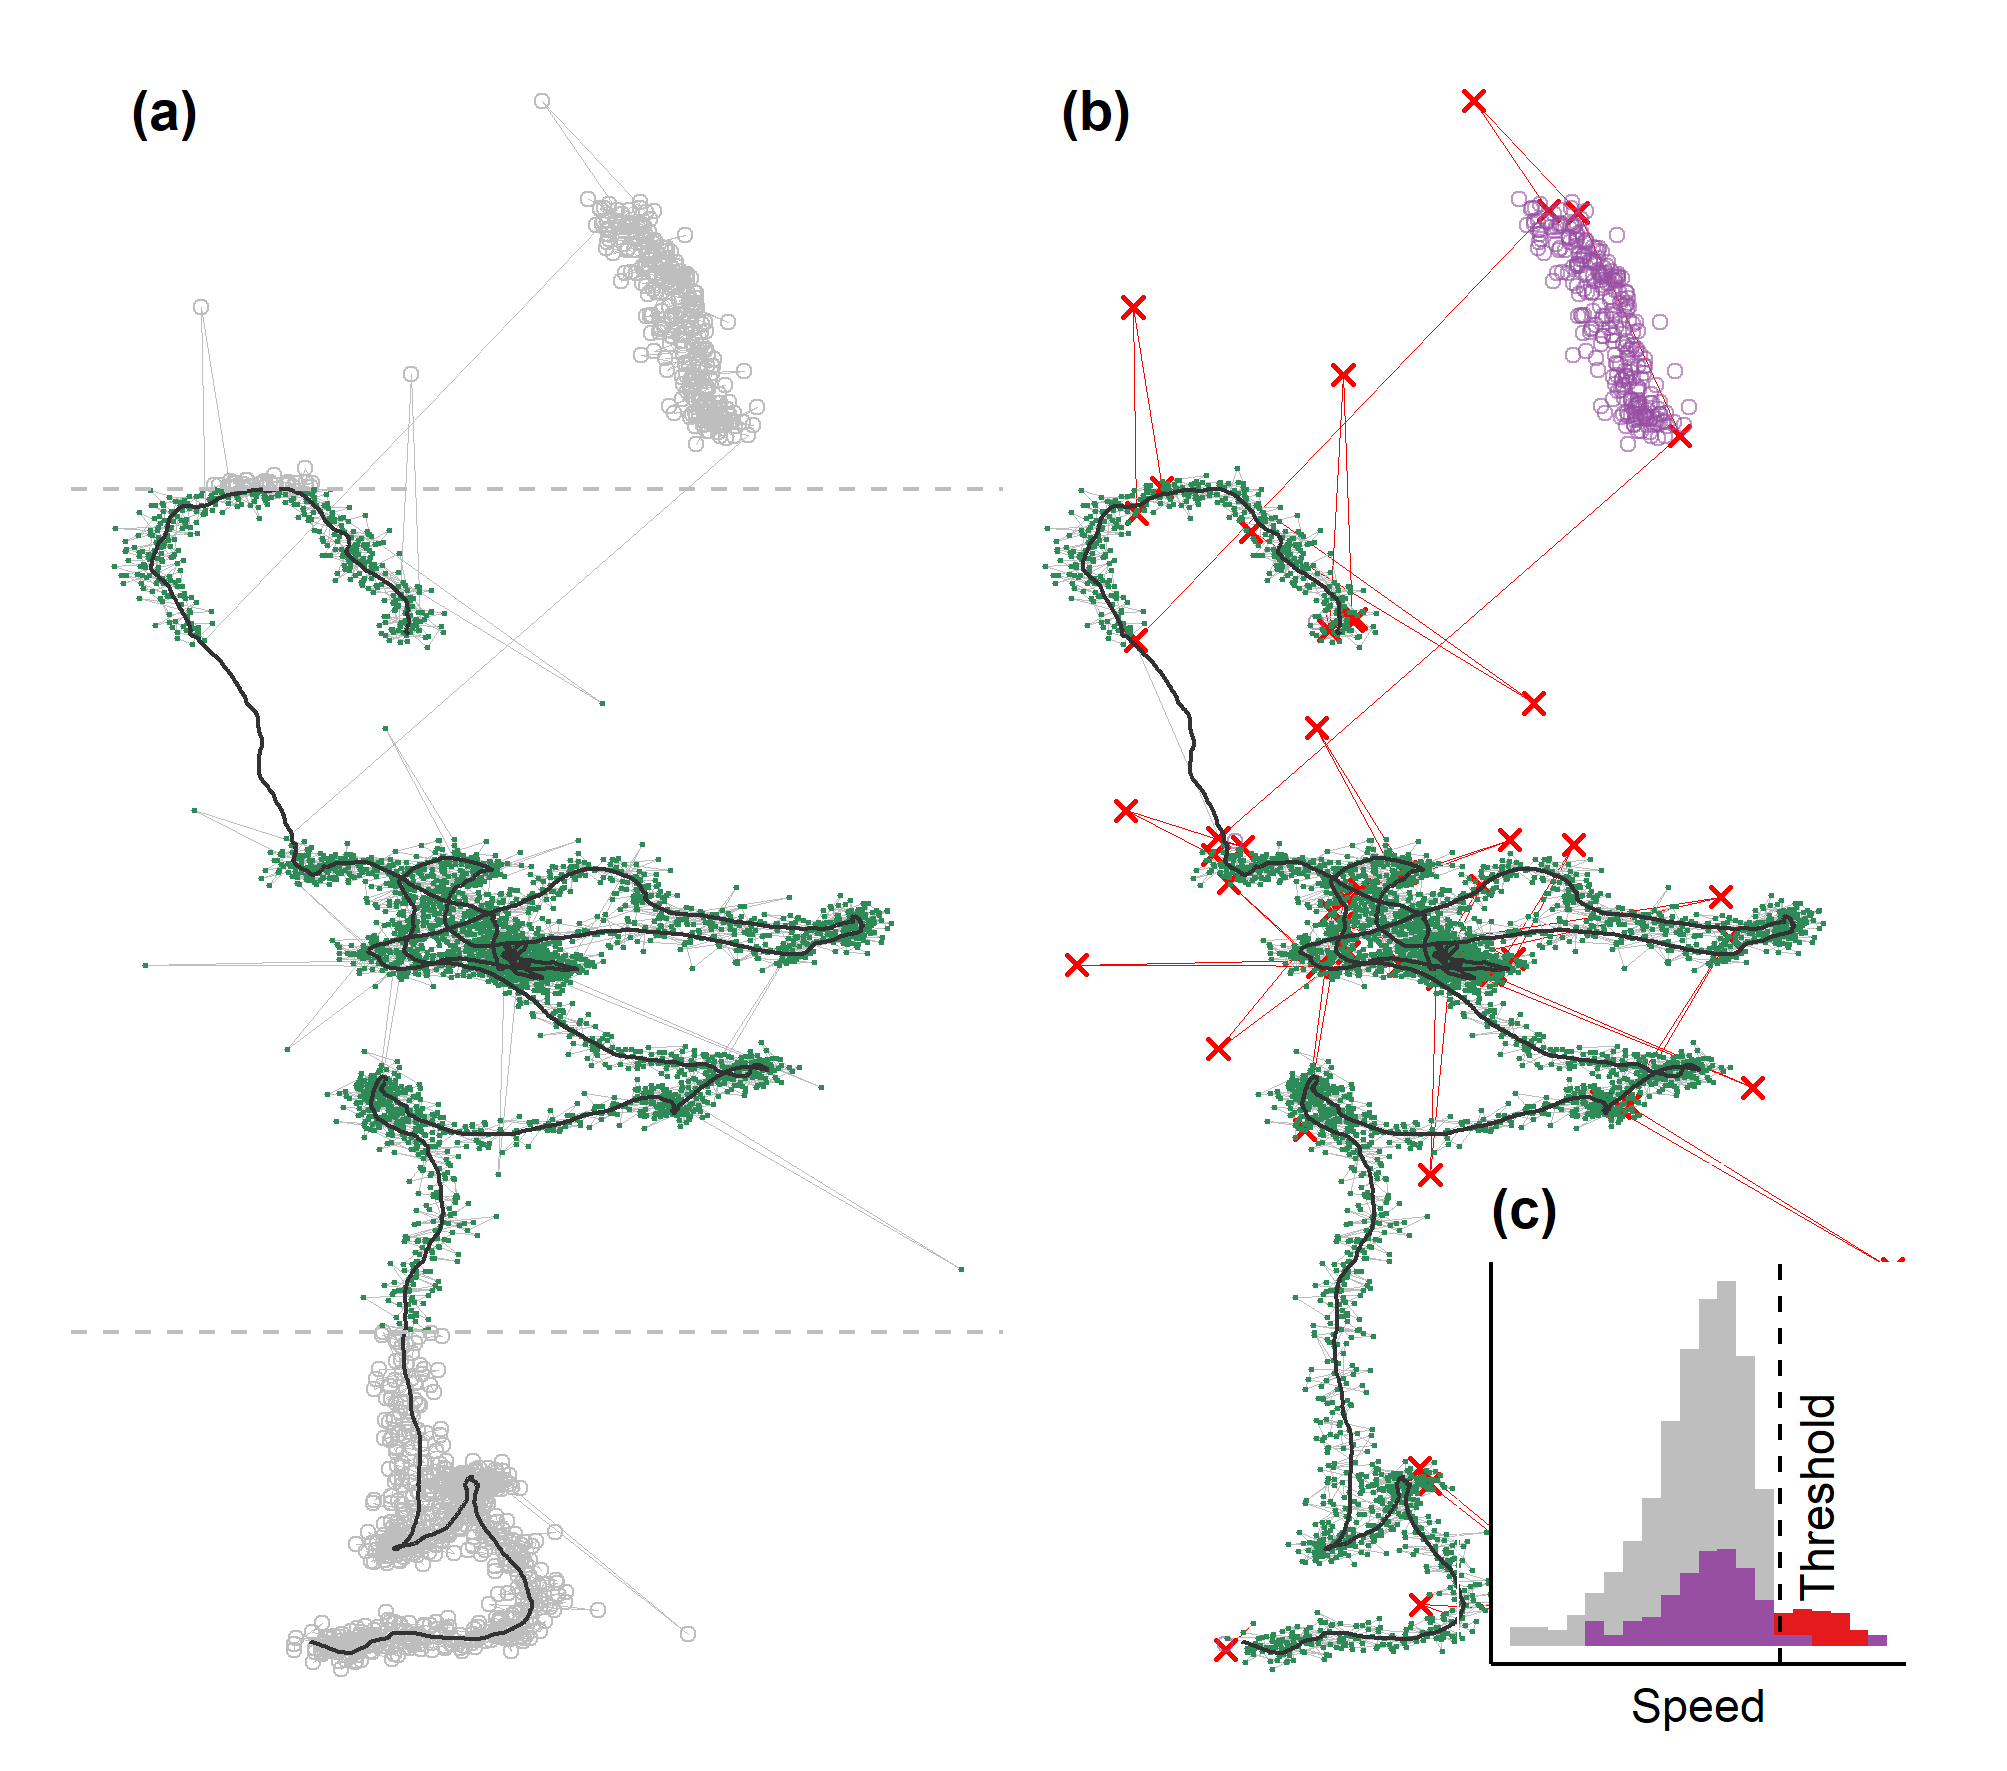
\includegraphics[width=0.9\textwidth]{figures/preprocessing/fig_03.png}
    \caption{
        \textbf{Simulated movement data showing four kinds of artificially added errors}.
        (i) Normally distributed small-scale error on each position, (ii) large-scale error added to 0.5\% of positions, (iii) 10\% of positions removed to simulate missing data, and (iv) 300 consecutive positions displaced to simulate a gross distortion affecting a continuous subset of the track.
        \textbf{(a)} Tracks can be quickly filtered by spatial bounds (dashed grey lines) to exclude broad regions (green = retained; grey = removed).
        \textbf{(b)} location error may affect single observations resulting in point outliers or `spikes' (red crosses and track segments), or continuous subsets of a track, called a `prolonged spike' (purple circles, top right), and both represent unrealistic movement.
        \textbf{(c)} Histograms of speed for the track (grey = small-scale errors, red = spikes), and the prolonged spike (purple) show that while spikes could be removed by filtering out positions with both high incoming and outgoing speeds and turning angles, prolonged spikes cannot be removed in this way, and should be resolved by conceptualising algorithms that find the bounds of the distortion instead.
        Users should frequently check the outputs of such algorithms to avoid rejecting valid data.
    }
    \label{preproc_fig_03}
\end{figure}

\subsection*{Temporal and Spatio-temporal Filters}

Tracking data might fail to properly represent an animal's movement at certain times, for instance, data recorded before release, or data from shortly after release when the animal is still influenced by the stress of capture and handling.
Periods of poor tracking quality may result from system malfunctions and unusual disturbances, and users may wish to exclude these data as well.
Temporal filtering can exclude positions from intervals when data are expected to be unreliable for ecological inference, either due to abnormal movement behaviour or system-specific issues.  
Temporal filters can be combined with spatial filters to select specific time-location combinations. 
For example, studies of foraging behaviour of a nocturnal animal would typically exclude tracking data from the animal's daytime roosts (see \textit{Worked Out Example}).
Users should apply filters in sequence rather than all at once, and visualise the output after each filtering step (`sanity checks'; see Supplementary Material Section 2).
The atlastools function \textit{atl\_filter\_covariates} allows convenient filtering of a dataset by any number of logical statements, including querying data within a spatio-temporal range.
% This function can be used to easily filter timestamps in a range, as well as combine simple spatial and temporal filters.
% It accepts a character vector of \textit{R} expressions that each return a logical vector (i.e., \textit{TRUE} or \textit{FALSE}; {\color{red} Listing} 2).
The function keeps only those data which satisfy each of the filter conditions, and users must ensure that the filtering variables exist in their dataset in order to avoid errors.

% \begin{lst{\color{red} Listing}}[float, language=R, style=customR, caption = {
%     Data can be filtered by a temporal or a spatio-temporal range using \textit{atl\_filter\_covariates}. 
%     Filter conditions are passed to the \textit{filters} argument as a character vector. 
%     Only rows in the data satisfying \textit{all} the conditions are retained. 
%     Here, the first example shows how nighttime data can be retained using a predicate that determines whether the value of `hour' is between 6 and 18, and also within a range of X coordinates.
%     The second example retains ATLAS locations calculated using $>$ 3 base stations (\textit{NBS}), with location error (\textit{SD}) $<$ 100, and data between an arbitrary day 5 and day 8.
%     }]
% night_data <- atl_filter_covariates(
%                     data = dataset,
%                     filters = c(
%                         "!inrange(hour, 6, 18)",
%                         "between(x, x_min, x_max)"
%                     )
%                 )

% filtered_data <- atl_filter_covariates(
%                         data = data,
%                         filters = c(
%                             "NBS > 3",
%                             "SD < 100",
%                             "between(day, 5, 8)"
%                         )
%                     )                            
% \end{lst{\color{red} Listing}}

\section*{Filtering to Reduce Location Errors}

\subsection*{Filtering on Data Quality Attributes}

Tracking data attributes can be good indicators of the reliability of positions calculated by a tracking system \citep{beardsworth2022mee}.
GPS systems provide direct measures of location error during localisation \citep[Horizontal Dilution of Precision, HDOP in GPS]{ranacher2016}, while  in reverse-GPS systems, a measure referred to as Standard Deviation (SD in many datasets), can be calculated from the variance-covariance matrix of each position as: $\text{SD} = \sqrt{\text{Var X} + \text{Var Y} + \text{Cov XY}}$ \citep[see details in][]{maccurdy2009, maccurdy2019, weiser2016, ranacher2016}.
Tracking data can also include indirect indicators of data quality.
For instance, GPS systems' location error may be indicated indirectly by the number of satellites involved in the localisation.
In reverse-GPS systems too, the number of base stations involved in each localisation is an indirect indicator of data quality, and positions localised using more receivers are usually more reliable \citep[the minimum required for an ATLAS localisation is 3; see][]{weiser2016,beardsworth2022mee}.
A location error measure associated with each coordinate pair (similar to GPS HDOP) can be calculated and assigned to a new column \textit{SD} using the formula for the sum of correlated random variables
\begin{linenomath*}
    \begin{equation*}
        SD = \sqrt{{VARX} + {VARY} + 2 \times {COVXY}}
     \end{equation*}
\end{linenomath*}
Unreliable positions can be removed by filtering on direct or indirect measures of quality using \textit{atl\_filter\_covariates}.
While filtering on direct quality attributes and unrealistic movement speeds (see below) will often be sufficient, filtering on indirect quality indicators is a strategy to consider when direct error measures are not available.

\subsection*{Filtering Unrealistic Movement}

Filtering on system-generated attributes may not remove all erroneous positions, and the remaining data may still include biologically implausible movement.
Users are encouraged to visualise their tracks before and after filtering point locations, and especially to `join the dots' and connect consecutive positions with lines (Fig.~\ref{preproc_fig_03}.b).
Whether the resulting track looks realistic is ultimately a subjective human judgement, but any decision to filter-out data must remain independent of the hypothesised movement behavior.
This basic principle does not preclude explicitly integrating prior knowledge of the movement ecology of the study species to ask, `Does the animal move this way?'.
Segments which appear to represent unrealistic animal movement are often obvious to researchers with extensive experience of the study system \citep[the non-movement approach; see][]{bjorneraas2010}.
Since it is both difficult and prohibitively time consuming to exactly reproduce expert judgement when dealing with large volumes of tracking data from multiple individuals, some automation is necessary.
Users should first manually examine a representative subset of tracks and attempt to visually identify problems --- either with individual positions, or with subsets of the track --- that persist after filtering on system-generated attributes.
Once such problems are identified, users can conceptualise algorithms that can be applied to their data to resolve them.

A common example of a problem with individual positions is that of point outliers or `spikes' \citep{bjorneraas2010}, where a single position is displaced far from the track (see Fig.~\ref{preproc_fig_03}.b).
Point outliers are characterised by artificially high speeds between the outlier and the positions before and after \citep[called incoming and outgoing speed, respectively;][]{bjorneraas2010}, lending a `spiky' appearance to the track.
Removing spikes is simple: remove positions with extreme incoming and outgoing speeds.
Users must first define plausible upper limits of the study species' speed \citep{calenge2009, seidel2018}.
Here, it is important to remember that speed estimates are scale-dependent; high-throughput tracking typically overestimates the speed between positions where the animal is stationary or moving slowly, due to small-scale location errors \citep{ranacher2016, noonan2019}. 
Even after data with large location errors have been removed, it is advisable to begin with a liberal (high) speed threshold that excludes only the most unlikely speeds.
Estimates of maximum speed may not always be readily obtained for all species, and an alternative is to use a data-driven threshold such as the 90\textsuperscript{th} percentile of speeds from the track.
Once a speed threshold $S$ has been chosen, positions with incoming \textit{and} outgoing speeds $> S$ may be identified as spikes and removed.

Some species can realistically achieve speeds $> S$ in fast transit segments when assisted by their environment, such as birds with tailwinds, and a simple filter on incoming and outgoing speeds would exclude this valid data.
To avoid removing valid, fast transit segments while still excluding spikes, the speed filter can be combined with a filter on the turning angles of each position \citep[see][]{bjorneraas2010, calenge2009}.
This combined filter assumes that positions in high-throughput tracking with both high speeds and large turning angles are likely to be due to location errors, since most species are unable to turn sharply at very high speed.
Users can then remove those positions whose incoming and outgoing speeds are both $> S$, and where $\theta > A$ (sharp, high-speed turns), where $\theta$ is the turning angle, and $A$ is the turning angle threshold.
Many other track metrics may be used to identify implausible movement and to filter data \citep{seidel2018}.
At this early stage in pre-processing, track metrics should be considered provisional --- it is not until after smoothing and potentially resampling to a regular interval (see below), that calculated track metrics should be used for ecological inference.
% We show an implementation of spike removal using the \textit{atl\_filter\_covariates} function.

% \begin{lst{\color{red} Listing}}[float, language=R, style=customR, caption = {
%     Filtering a movement track on incoming and outgoing speeds, and on turning angle to remove unrealistic movement.
%     The functions \textit{atl\_get\_speed} and \textit{atl\_turning\_angle} are used to get the speeds and turning angles before filtering, and assigned to a column in the data (assignment of \textit{speed\_out} is not shown).
%     The filter step only retains positions with speeds below the speed threshold $S$ \textit{or} angles above the turning angle threshold $\theta$, i.e., positions where the animal is slow but makes sharp turns, and data where the animal moves quickly in a relatively straight line.}]
% data$speed_in <- atl_get_speed(
%                     data,
%                     x = "x", y = "y",
%                     time = "time", 
%                     type = c("in")
%                 )

% data$angle <- atl_turning_angle(
%                     data,
%                     x = "x", y = "y", 
%                     time = "time"
%                 )

% filtered_data <- atl_filter_covariates(
%                     data = data,
%                     filters = c(
%                         "(speed_in < S & speed_out < S) | angle < A"
%                     )
%                 )
% \end{lst{\color{red} Listing}}

Sometimes, entire subsets of the track may be affected by the same large-scale location error.
For instance, multiple consecutive positions may be roughly translated (geometrically) away from the real track and form `prolonged spikes', or `reflections' (see Fig.~\ref{preproc_fig_03}.b).
These cannot be corrected by targeted removal of individual positions, as in Bjørneraas et al.'s approach (2010), since there are no positions with both high incoming and outgoing speeds, as well as sharp turning angles, that characterise spikes.
Since filtering individual positions will not suffice, algorithms to correct such errors must take a track-level view, and target the displaced sequence overall.
Track-subset algorithms are likely to be system-specific, and may be challenging to conceptualise or implement.
In the case of prolonged spikes, one relatively simple solution is identifying the bounds of displaced segments, and removing positions between them.
This identification can be based on relatively simple rules --- for example, the beginning of a prolonged spike could be identified as a position with a high \textit{incoming} speed, but a low \textit{outgoing} speed, while the end of such a spike would have a low incoming, but a high outgoing speed.
We have implemented an illustrative example of such an algorithm in the form of track-subset filtering for prolonged spikes using the \textit{atlastools} function \textit{atl\_remove\_reflections} (see the \textit{atlastools} documentation for details on the algorithm).
Users are strongly encouraged to visualise their data before and after applying such algorithms; as these methods are not foolproof, and data that are heavily distorted by errors affecting entire track-subsets should be used with care when making further inferences.

% % \begin{lst{\color{red} Listing}}[float, language=R, style=customR, caption = {
% %     Removing unrealistic movement in the form of prolonged spikes from a movement track. 
% %     The important function arguments here are \textit{point\_angle\_cutoff} ($A$), \textit{reflection\_speed\_cutoff} ($S$), and \textit{est\_ref\_len}, the maximum number of positions after the inner bound that are candidates for the end of the prolonged spike, i.e., the outer bound. 
% %     If the prolonged spike ends after less than $N$ positions, the true end point is used as the outer bound of the spike.
% %     However, the algorithm behind this function fails when the prolonged spike ends after more than $N$ positions. 
% %     Users are advised to use a liberally large value of N in the \textit{est\_ref\_len} argument; 1,000 may be appropriate for 3s interval data.
% %     Further, users are cautioned against relying on such algorithms for severely distorted data.}]
% % filtered_data <- atl_remove_reflections(data = track_data,
% %                        x = "x", y = "y", time = "time",
% %                        point_angle_cutoff = A,
% %                        reflection_speed_cutoff = S,
% %                        est_ref_len = N)
% % \end{lst{\color{red} Listing}}

\section*{Smoothing and Thinning Data}

\subsection*{Median Smoothing}

After filtering out large location errors, the track may still look `spiky' at small scales, and this is due to smaller location errors that are especially noticeable when the individual is stationary or moving slowly \citep{noonan2019}.
These smaller errors are challenging to remove since their attributes (such as speed and turning angles) are within the expected range of movement behaviour for the study species. 
The large data volumes of high-throughput tracking allow users to resolve this problem by smoothing the positions. 
The most basic `smooths' work by approximating the value of an observation based on neighbouring values.
For a one-dimensional series of observations, the neighbouring values are the $K$ observations centred on each index value $i$.
The range ${i - (K-1)/2} \ldots {i + (K-1)/2}$ is referred to as the moving window as it shifts with $i$, and $K$ is the moving window size.
A common smooth is nearest neighbour averaging, in which the value of an observation $x_i$ is the average of the moving window $K$.
The median smooth is a variant of nearest neighbour averaging which uses the median rather than the mean, and is more robust to outliers (\citeauthor{tukey1977} 1977).
The median smoothed value of the X coordinate, for instance, is
%
% \begin{linenomath*}
    % \begin{equation*}
    $$
        X_i = \text{Median}(X_{i - (K-1)/2} \ldots X_{i + (K-1)/2}).
    $$
        % \end{equation*}
% \end{linenomath*}
Users can apply a median smooth with an appropriate $K$ independently to the X and Y coordinates of a movement track to smooth it (see Fig.~\ref{preproc_fig_04}.a -- e).
The median smooth is robust to even very large temporal and spatial gaps, and does not interpolate between positions when data are missing. 
Thus it is not necessary to split the data into segments separated by periods of missing observations when applying the filter (see Fig.~\ref{preproc_fig_04}).

Some data sources, such as GPS, provide tracks that have already been smoothed in quite sophisticated ways, such as with a Kalman filter, making a median smooth unnecessary \citep{kaplan2005}.
Furthermore, smoothing is not a panacea for data quality issues, and has its drawbacks.
Smoothing does not change the number of observations, but does decouple the coordinates from some of their attributes.
For instance, smoothing breaks the relationship between a coordinate and the location error estimate around it (VARX, VARY, and SD in ATLAS systems).
Since the X and Y coordinates are smoothed independently, the smoothed coordinates of an observation will likely differ from all the coordinates used to compute the smoothed value.
Any position covariates (e.g. environmental values such as landcover or elevation) obtained before smoothing should be replaced with the covariates obtained at the smoothed coordinates.
Similarly, instantaneous track metrics, such as speed and turning angle, should also be updated at this stage to reflect the smoothed coordinates.
Furthermore, the location error estimate around each coordinate, and around the localisation overall, become invalid and should be ignored.
This makes subsequent filtering on measures of data quality unreliable, and smoothed data are unsuitable for use with methods that model location uncertainty \citep{noonan2019, fleming2014, fleming2020, calabrese2016}.
Thus, when applying location error modelling methods, users should ensure that the error measure bears a mechanistic relationship with the location estimate \citep[see][ for more details]{fleming2020, noonan2019}.
Additionally, excessively large $K$ may result in a loss in detail of the individual's small-scale movement (compare Fig.~\ref{preproc_fig_04}.e with ~\ref{preproc_fig_04}.a).
Users must themselves judge how best to balance large-scale and small-scale accuracy, and choose $K$ accordingly.
Median smoothing is provided by the \textit{atlastools} function \textit{atl\_median\_smooth}, with the only option being the moving window size, which must be an odd integer.

% \begin{lst{\color{red} Listing}}[float, language=R, style=customR, caption = {
%     Median smoothing a movement track using the function \textit{atl\_median\_smooth} function with a moving window \textit{K = 5}. 
%     Larger values of $K$ yield smoother tracks, but $K$ should always be some orders of magnitude lower than the number of observations.}]
% atl_median_smooth(
%     data = track_data,
%     x = "x", y = "y",
%     time = "time",
%     moving_window = 5
% )
% \end{lst{\color{red} Listing}}

\begin{figure}[ht!]
    \centering
    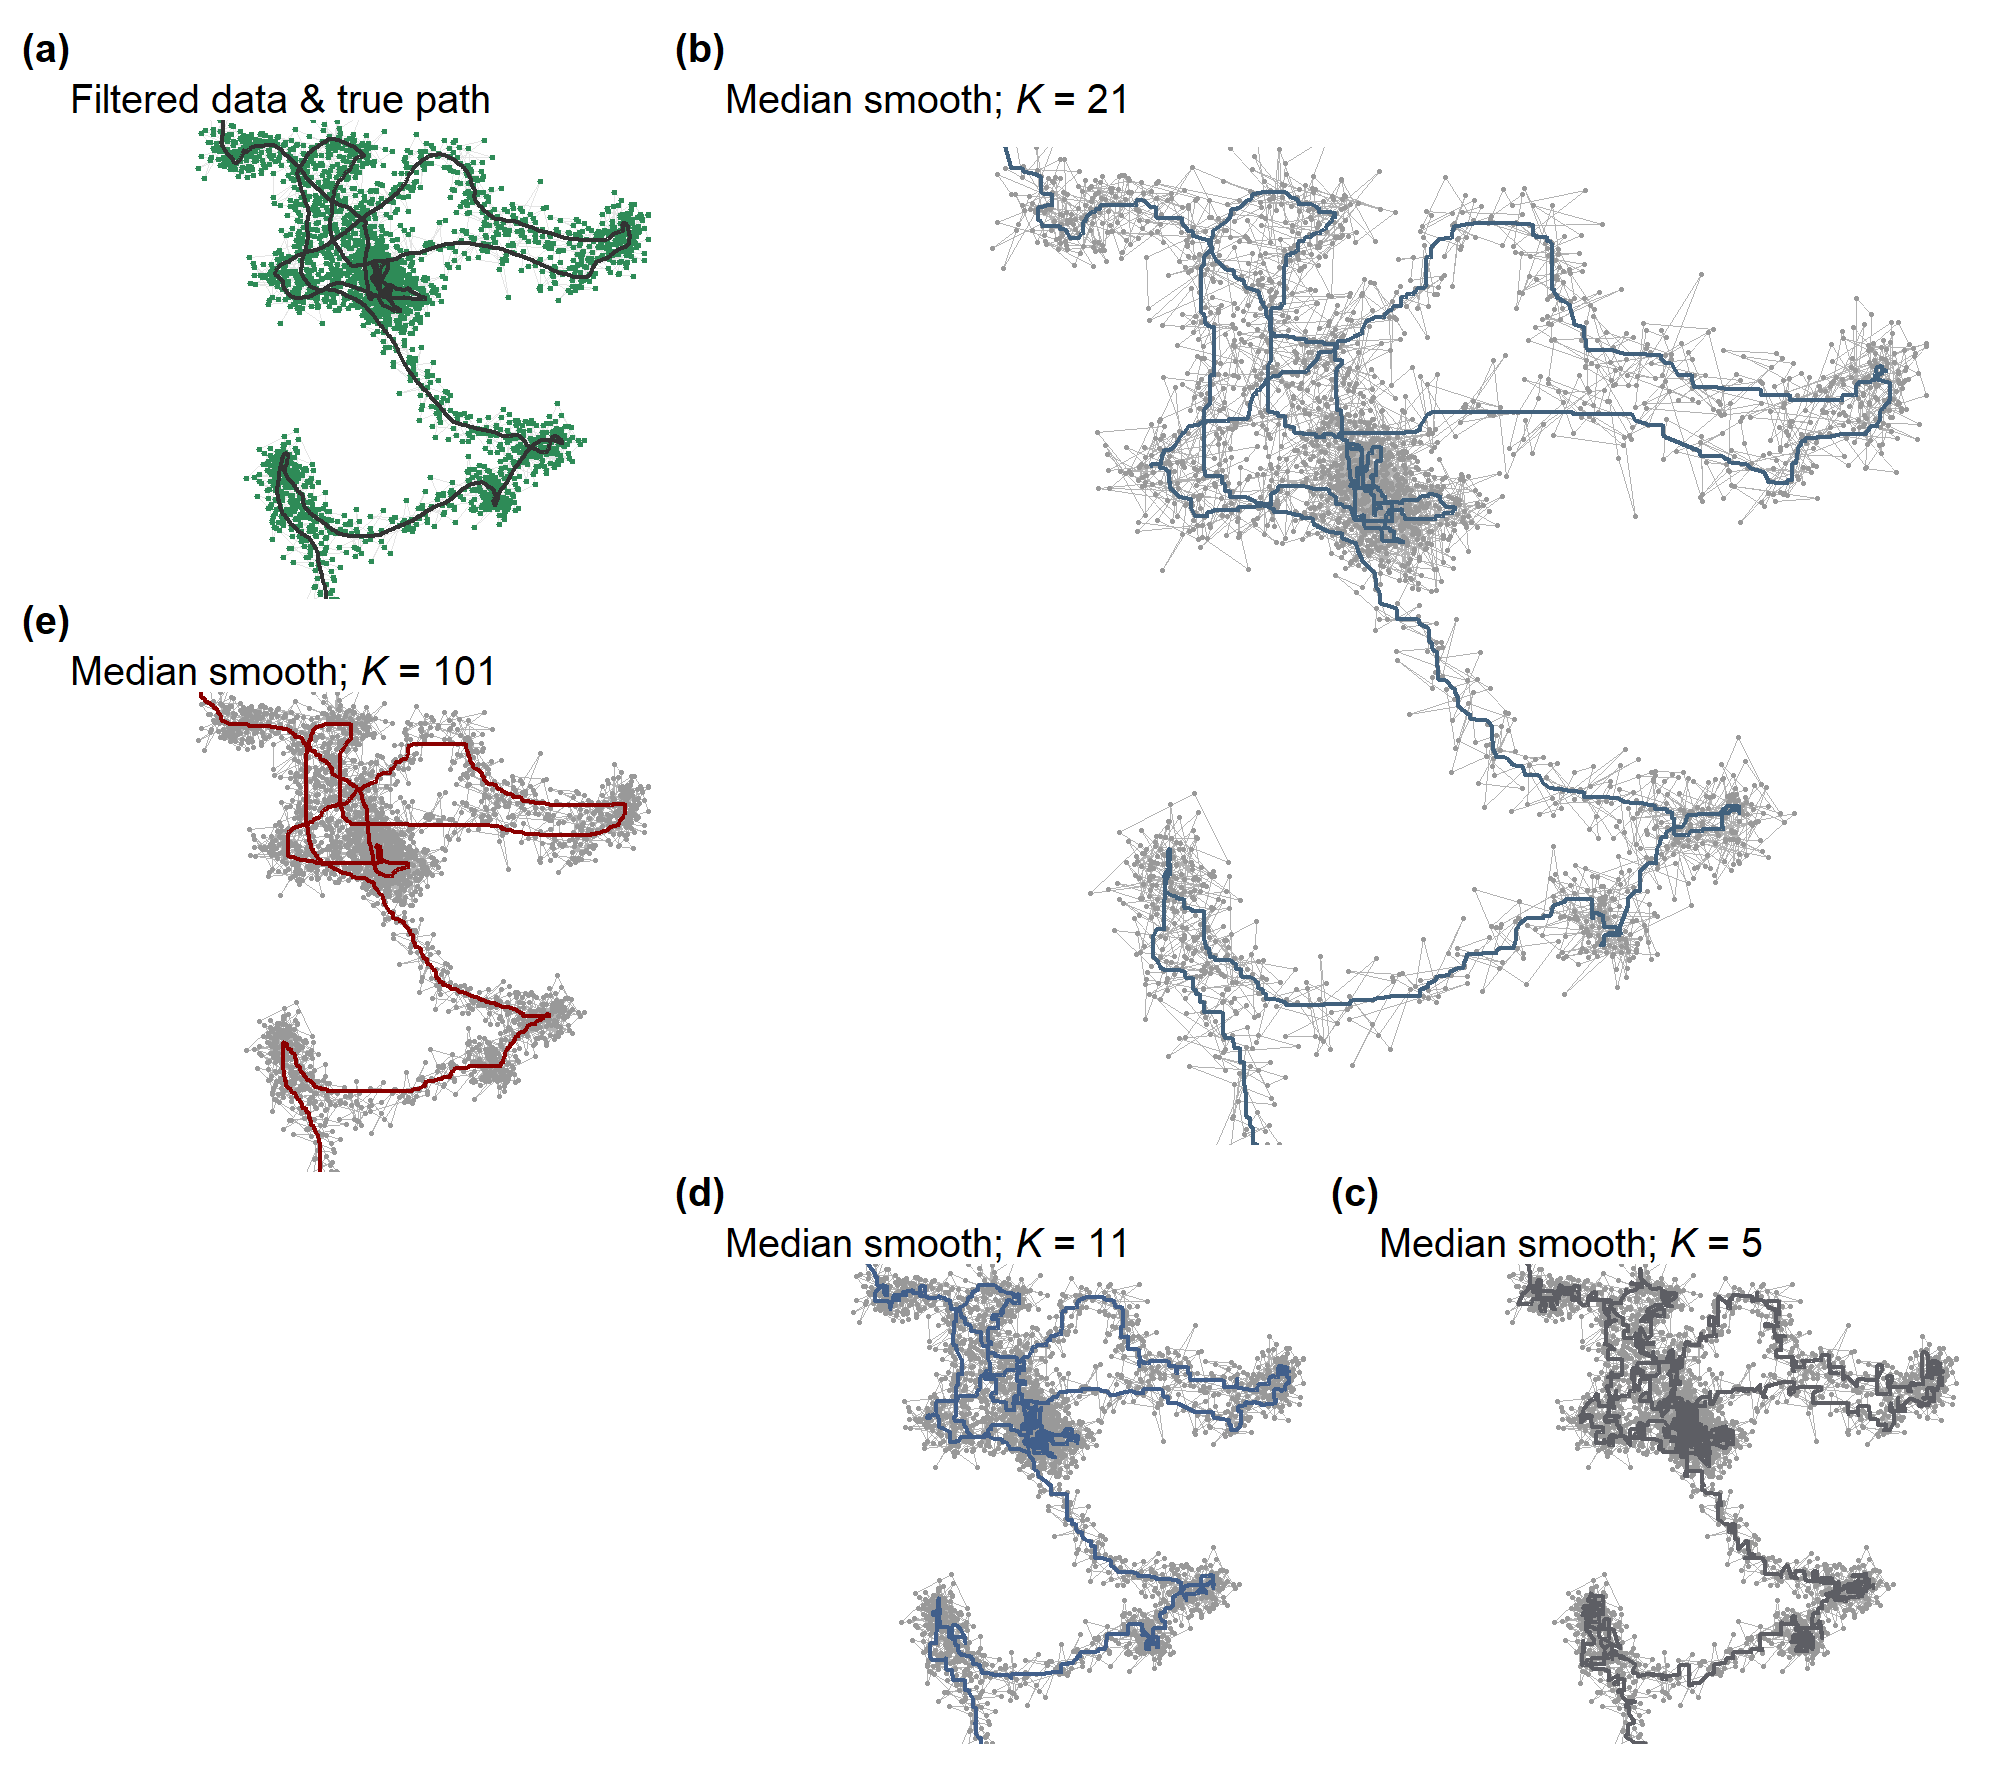
\includegraphics[width=0.9\textwidth]{figures/preprocessing/fig_04.png}
    \caption{
        \textbf{Median smoothing position coordinates reduces small-scale location error in tracking data.}
        The goal of this step is to approximate the simulated canonical track (black line, \textbf{(a)}), given positions with small-scale error that remains after filtering in previous steps (green points).
        \textbf{(b)} Median smoothing the position coordinates (green points, in \textbf{(a)}) over a moving window ($K$) of 21 positions gives a good approximation (blue line) of the canonical track, and is a significant improvement on the unsmoothed track (grey lines and points).
        While $K$ should usually be at least two orders of magnitude less than the number of positions in the track, users are cautioned that there is no correct $K$, and they must subjectively choose a $K$ which most usefully trades small-scale details of the track for large-scale accuracy.
        Here, smoothing with a $K$ of \textbf{(c)} 5 (dark grey line) and \textbf{(d)} 11 (blue line), leads to a jagged track, compared to the true path in (a), and the distance moved by the animal would be overestimated.
        \textbf{(e)} Using extremely large values of $K$ (101) may lead to a loss of both large and small scale detail (red line).
        Across panels, grey lines and points show the track without smoothing.
    }
    \label{preproc_fig_04}
\end{figure}

\subsection*{Thinning Movement Tracks}

Most data at this stage are technically ‘clean', yet the volume alone may pose challenges for lower-specification or older hardware and software if these are not optimised for efficient computation.
Thinning data i.e., reducing their volume, need not compromise researchers' ability to answer ecological questions; for instance, proximity-based social interactions lasting 1 -- 2 minutes would still be detected on thinning from a sampling interval of 1 second to 1 minute \citep[][]{aspillaga2021a}.
Thinning data also does not imply that efforts to collect high-throughput movement data are ‘wasted', as rich movement datasets enable more detailed and more accurate representation of the true track, as elaborated above. 
Indeed, some analyses require that temporal auto-correlation in the data be broken by subsampling the data to a lower resolution; these include traditional kernel density estimators for animal home-range, as well as resource selection functions \citep{fleming2014,manly2007,dupke2017}.
Furthermore, a number of powerful methods in movement ecology, including Hidden Markov Models and integrated Step-Selection Analysis recommend uniform sampling intervals \citep{avgar2016,langrock2012,michelot2016}.
Finally, subsampling data may be an important strategy in exploratory data analysis; for instance, it allows researchers to determine whether computationally intensive methods, such as distance and speed estimates from continuous time movement model fitting, are required for their data, or whether the movement metrics stabilise at a certain time scale \citep[][]{noonan2019}.
Two plausible approaches here are subsampling and aggregation, and both approaches begin with identifying time-interval groups (e.g. of 1 minute).
Subsampling picks one position from each time-interval group while aggregation involves computing the mean or median of all system-generated attributes for positions within a time-interval group.
Here again, users should repeat the extraction of any environmental covariates for the thinned data, and may wish to obtain the mean values in a radius aroung the locations, rather than point estimates alone.
Both approaches yield one position per time-interval group (Fig.~\ref{preproc_fig_05}.a).
Categorical variables, such as the habitat type associated with each position, can be aggregated using a suitable measure such as the mode.
We caution users that thinning causes an extensive loss of small-scale detail in the data, and should be used carefully.

Both aggregation and subsampling have their relative advantages. 
The aggregation method is less sensitive to selecting point outliers by chance than subsampling.
However, to account for location error with methods such as state-space models \citep{jonsen2003, jonsen2005, johnson2008} or continuous time movement models \citep{fleming2014, noonan2019, gurarie2017, calabrese2016, fleming2020}, correctly propagating the location error is important, and subsampling directly propagates these errors without further processing.
In reverse-GPS systems systems the location error is calculated from the variance-covariance matrix of the coordinates of candidate positions considered by the location solver \citep{weiser2016}; this is equivalent to GPS systems' HDOP \citep{ranacher2016}.
In the aggregation method, the location error around each coordinate provided by either GPS or reverse-GPS systems can be propagated --- assuming the errors are normally distributed --- to the averaged position as the sum of errors divided by the square of the number of observations contributing to each average ($N$):
% \begin{linenomath*}
    $$
        \text{Var}(X)_\text{agg} = \left( \sum_{i=1}^{i=N} \text{Var}(X)_i \right) / N ^ 2
    $$
% \end{linenomath*}
Similarly, the overall location error estimate for the average of $N$ positions in a time-interval can be calculated by treating it as a variance. For instance, the ATLAS error and GPS error measures (SD and HDOP, respectively) can be aggregated as:
% \begin{linenomath*}
    $$
        \text{SD}_\text{agg} \ or \ \text{HDOP}_\text{agg} = \sqrt{ \left( \sum_{i=1}^{i=N} \text{SD}_i^2 \ or \ \text{HDOP}_i^2 \right) / N ^ 2  }
    $$
% \end{linenomath*}

Users may question why thinning, which can obtain consensus positions over an interval and also reduce data-volumes should not be used directly on the raw data.
%%
We caution that thinning prior to excluding unrealistic movement and smoothing (Fig 5.b) can lead to preserving artefacts in the data, and estimates of essential metrics --- such as straight-line displacement (and hence, speed) --- that are substantially different from the true value \citep[see Fig.~\ref{preproc_fig_05}.c;][]{noonan2019}.
In our example, the data with errors would have to be thinned to $\frac{1}{30}$\textsuperscript{th} of its volume for the median speed of the thinned data to be comparable with the overall median speed --- this is an undesirable step if the aim is fine-scale tracking.
Additionally, the optimal level of thinning can be difficult to determine, especially if there is wide individual variation in movement behaviour, and the mis-estimation of track metrics from inappropriately thinned data could have consequences for the implementation of subsequent filters based on detecting unrealistic movement.
However, thinning before data-cleaning has its place as a useful step before exploratory visualisation of the movement track, since reduced data-volumes are easier to handle for plotting software.
%
Thinning is implemented in \textit{atlastools} using the \textit{atl\_thin\_data} function, with either aggregation or subsampling (specified by the \textit{method} argument) over an interval using the \textit{interval} argument.
Grouping variable names (such as animal identity) may be passed as a character vector to the \textit{id\_columns} argument.

% \begin{lst{\color{red} Listing}}[float, language=R, style=customR, caption = {Code to thin data by aggregation in \textit{atlastools}. The method can be either "aggregate" or "subsample". 
% The time interval is specified in seconds, while the \textit{id\_columns} allows a character vector of column names to be passed to the function, with these columns used as identity variables.
% Both methods return a dataset with one rows per time-interval.}]
% thinned_data <- atl_thin_data(
%                     data,
%                     interval = 60,
%                     id_columns = c("animal_id"),
%                     method = "aggregate"
%                 )
% \end{lst{\color{red} Listing}}

% % figure for aggregation thinning
\afterpage{
    \begin{sidewaysfigure}[p]
        \centering
        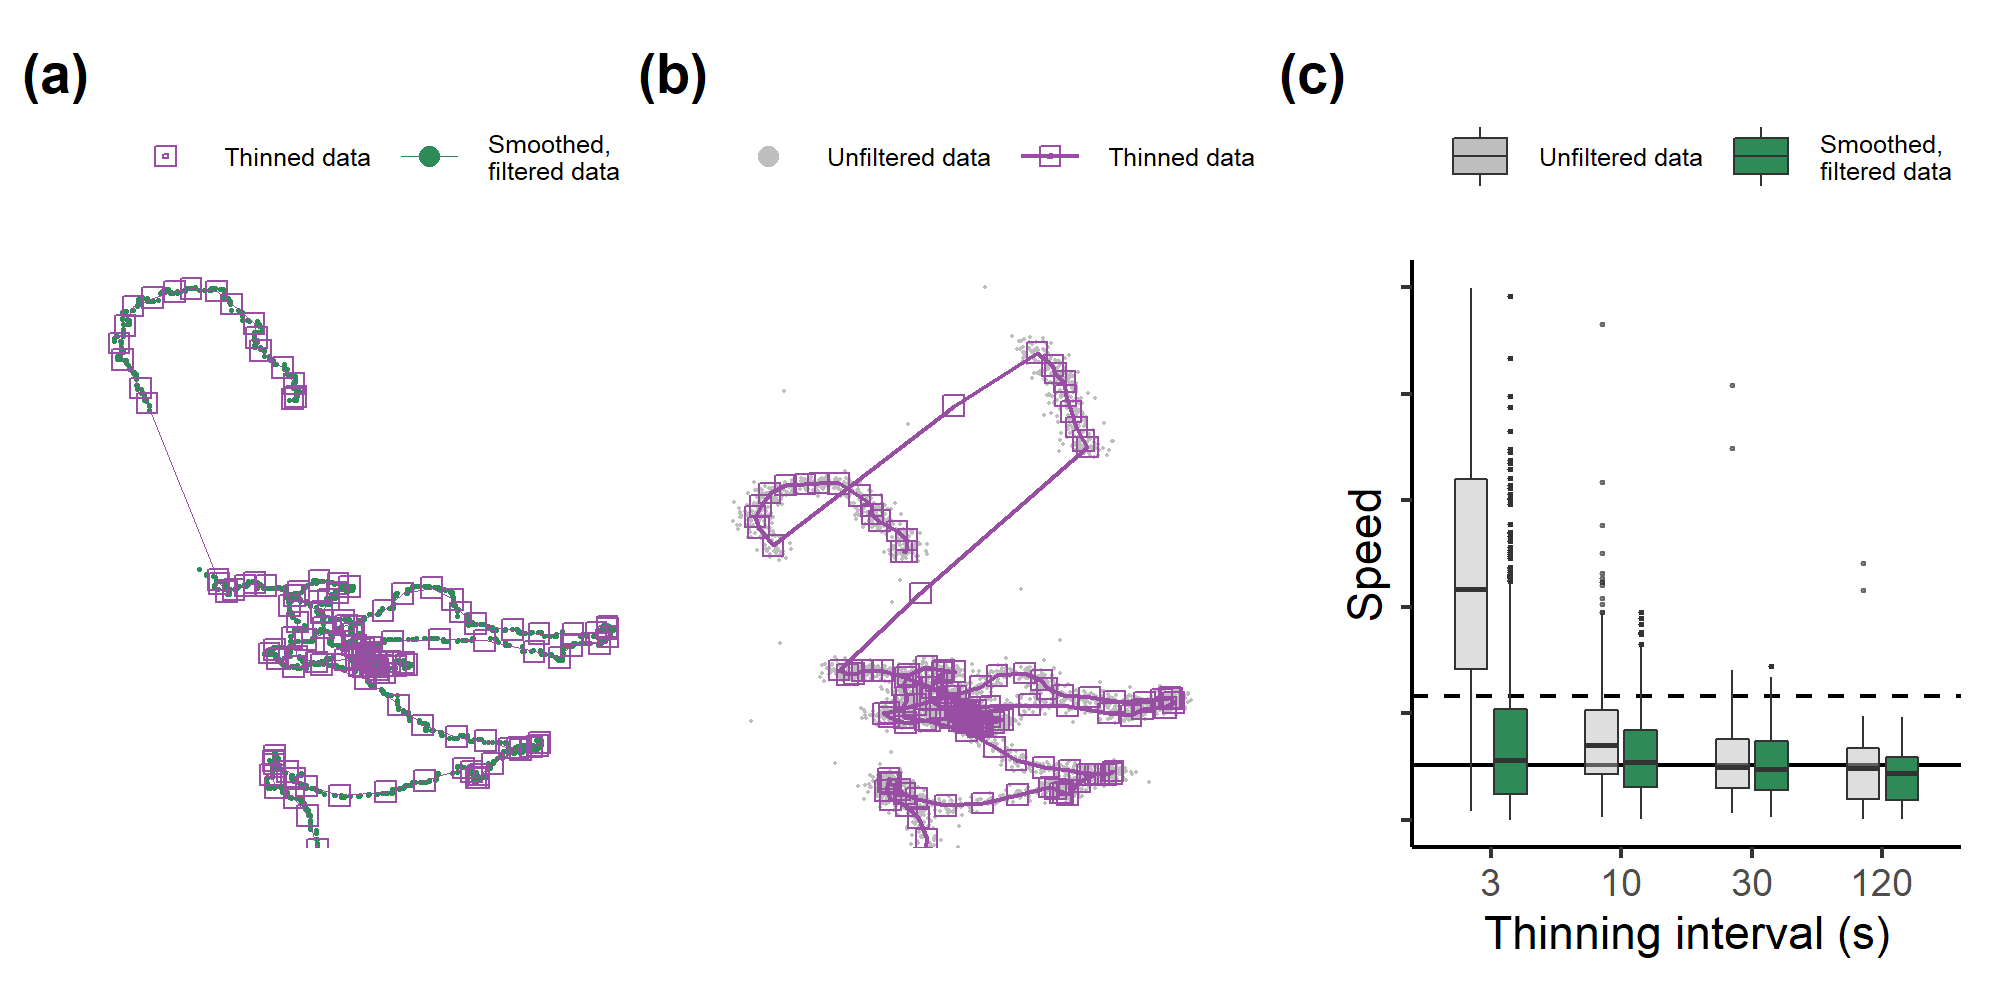
\includegraphics[width=0.7\textwidth]{figures/preprocessing/fig_05.png}
        \caption{
            \textbf{Thinning tracking data can aid computation but must be approached carefully}.
            Aggregating a filtered and smoothed movement track \textbf{(a)} preserves track structure while reducing data-volume, but \textbf{(b)} aggregating before filtering gross location errors and unrealistic movement leads to the persistence of large-scale errors (such as prolonged spikes).
            \textbf{(c)} Thinning before data cleaning can lead to significant misestimations of essential movement metrics such as speed at lower intervals.
            Boxplots show the median and interquartile ranges for speed estimates of tracks aggregated over intervals of 3, 10, 30, and 120 seconds.
            For comparison, the median and 95\textsuperscript{th} percentile of speed of the canonical track are shown as solid and dashed horizontal lines, respectively.
            % The unfiltered data would have to be thinned to \sfrac{1}{30}\textsuperscript{th} volume to correctly estimate median speed.
        }
        \label{preproc_fig_05}
    \end{sidewaysfigure}
}

\section*{System-Specific Pre-processing Tools}

When researchers' pre-processing requirements exceed the functionalities of existing tools, they might have to conceptualise and implement their own methods.
For instance, an important and common analysis with animal tracking data is to link space use with environmental covariates.
This is difficult even with smoothed and thinned high-throughput data, as these may be too large for statistical packages, or have strong autocorrelation.
Users aiming for such analyses can benefit from segmenting and clustering the data into spatio-temporally independent bouts of different behavioural modes \citep{patin2020a}.
Treating these as the unit of observation also conveniently sidesteps pseudo-replication and reduces computational requirements.
While numerous methods of segmenting and clustering data are in use, they may not be scalable to very large or gappy datasets \citep{patin2020a, langrock2012, michelot2016}.
As an alternative, a first-principles approach that segments data based on the movement capacity (top speed, etc.) of tracked animals, could provide a fast, yet useful way to cluster data.
Here, as a working example that may be suitable for some systems, we present a simple segmentation-clustering algorithm to make `residence patches', identified as bouts of relatively stationary behaviour \citep[][]{barraquand2008,bijleveld2016,oudman2018}.
Details of the implementation may be found in the package code, and examples are provided in the Supplementary Material.

\subsection*{Conceptualising a Simple Segmentation-Clustering Algorithm: The Residence-Patch Example}

Before implementing the algorithm, users should identify positions where the animal is relatively stationary, for instance on its speed or first-passage time \citep{bracis2018,barraquand2008}.
Our suggested algorithm begins by assessing whether consecutive stationary positions are spatio-temporally independent, and clusters them together into a residence patch if they are not.
This clustering could be based on a simple proximity threshold --- points farther apart than some threshold distance are likely to represent two different residence patches.
In cases where animals visit multiple sites in sequence \citep[such as traplining:][]{thomson1997}, and which researchers might wish to consider as a single residence patch, a larger-scale distance threshold can help cluster nearby residence patches together, and this can also be applied to cluster together patches artificially separated due to missing data.
Our algorithm separates two observations at a similar location, but at two very different time points, by comparing the intervening time-lag against a time-difference threshold, which can also apply to patches that would otherwise be clustered by the large-scale distance threshold.
Users are encouraged to base these thresholds on the movement habits of their study species (see the \textit{Worked Out Example}).

We have implemented a working example of the simple clustering concept presented here as the function \textit{atl\_res\_patch} (see Fig.~\ref{preproc_fig_06}.b), which requires three parameters: (i) the distance threshold between positions (called \textit{buffer\_size}), (ii) the large-scale distance threshold between clusters of positions (called \textit{lim\_spat\_indep}), and (iii) the time-difference threshold between clusters (called \textit{lim\_time\_indep}).
Clusters formed of fewer than a minimum number of positions can be excluded.
Our algorithm performs well when movement modes are clearly separated, and is capable of correctly separating positions that are close together in space and time, but which comprise different behavioural sequences (see Fig.~\ref{preproc_fig_06}).
While the algorithm may not cover all possible use-cases and study species, we provide it here as an example of a user-built exploratory method for animal tracking data.
It is important to systematically test such custom-made algorithms, to ensure reproducibility and reliability \citep{wickham2015, marwick2018}.
Simple examples of such tests for the residence patch method and other functions in \textit{atlastools} may be found in the \textit{tests/} directory in the associated Github repository.

% \begin{lst{\color{red} Listing}}[float, language=R, style=customR, caption ={The \textit{atl\_res\_patch} function can be used to classify a track into residence patches. The arguments \textit{buffer\_radius} and \textit{lim\_spat\_indep} are specified in metres, while the \textit{lim\_time\_indep} is provided in minutes. In this example, specifying \textit{summary\_variables = c("speed")}, and \textit{summary\_functions = c("mean", "sd")} will provide the mean and standard deviation of instantaneous speed in each residence patch. The \textit{atl\_patch\_summary} function is used to access the classified patch in one of three ways, here using the \textit{summary} option which returns a table of patch-wise summary statistics.}]
% patches <- atl_res_patch(
%                 data = track_data,
%                 buffer_radius = 10,
%                 lim_spat_indep = 100,
%                 lim_time_indep = 30,
%                 min_fixes = 3,
%                 summary_variables = c("speed"),
%                 summary_functions = c("mean", "sd")
%             )
% \end{lst{\color{red} Listing}}

% % patch_summary <- atl_patch_summary(
% %                     patch_data = patches,
% %                     which_data = "summary",
% %                     buffer_radius = 10
% %                 )

% % first residence patch figure
\begin{figure}[h!]
    \centering
    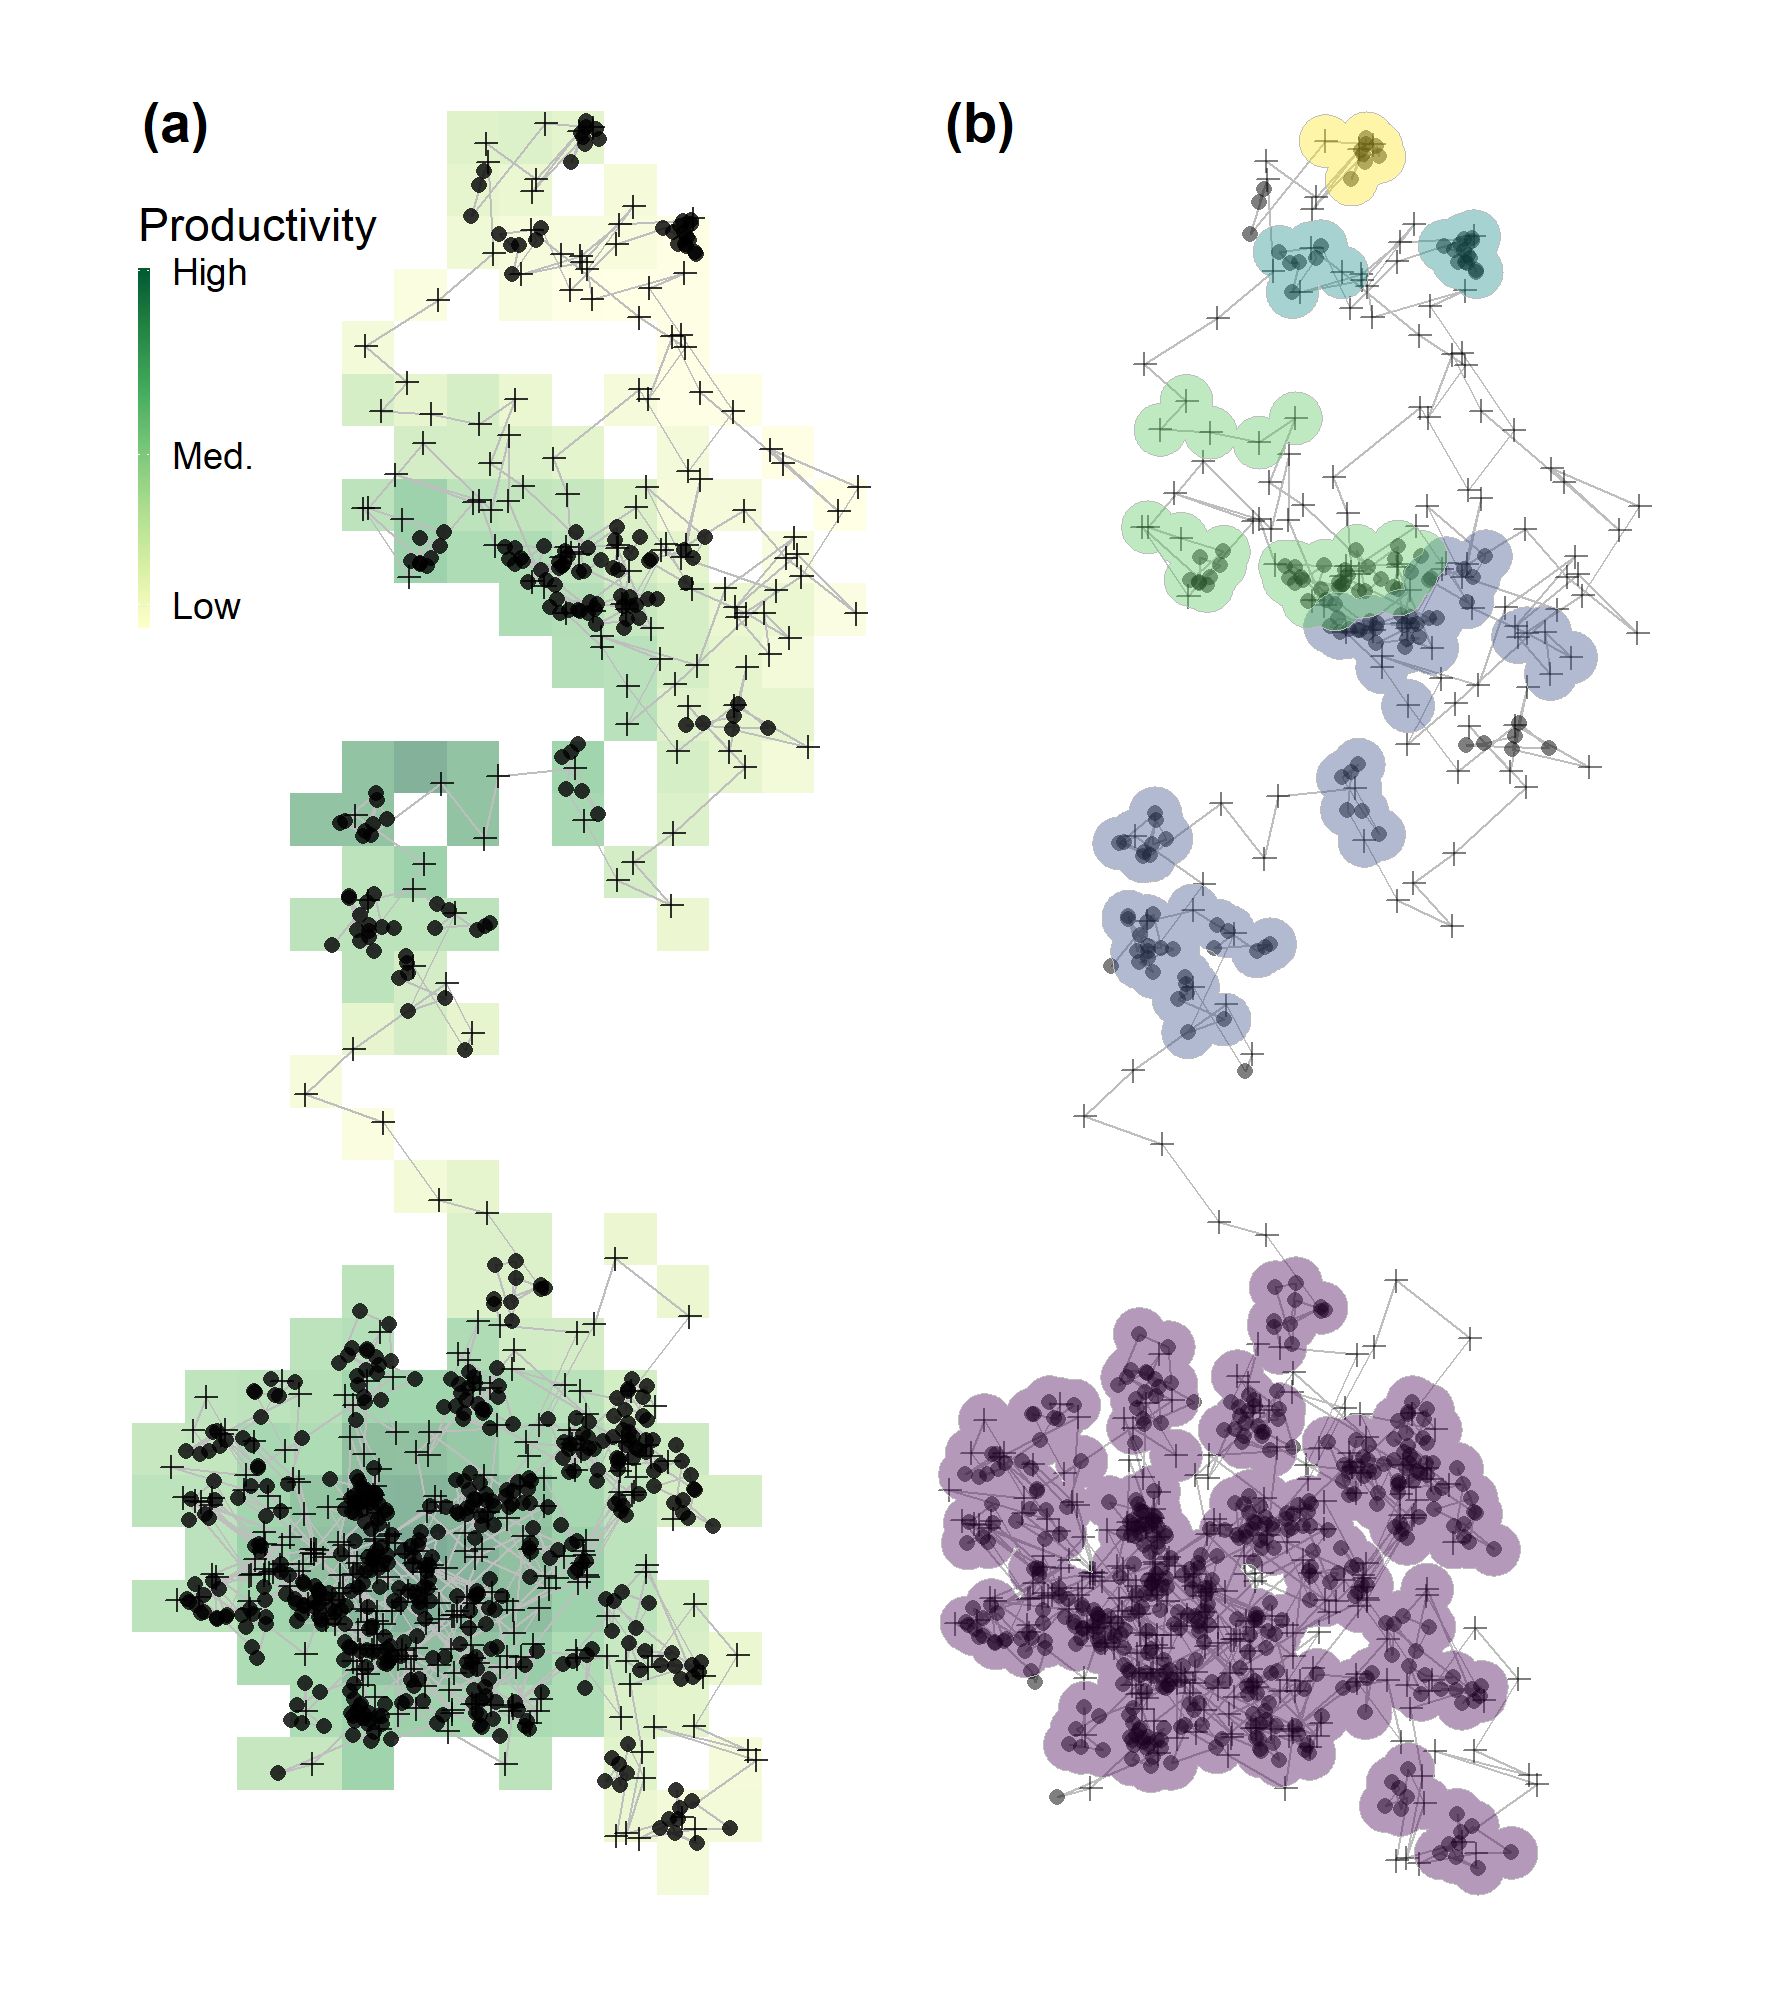
\includegraphics[width=0.75\textwidth]{figures/preprocessing/fig_06.png}
    \caption{
        \textbf{Movement tracks can be classified into residence patches, while leaving out the transit between them.}
        \textbf{(a)} A simulated animal movement track from \citealt{gupte2021a}, where an agent uses local cues to make movement decisions to maximise intake.
        The agent tends to stop (solid circles) on high-productivity areas of the landscape, as these are more likely to generate prey-items.
        Transit points between stationary phases are shown as crosses.
        \textbf{(b)} Our simple, first-principles based clustering algorithm classifies the track into five residence patches. 
        Some transit points are erroneously classified as being part of a residence patch (top, yellow), illustrating why is it important to remove such data before applying this method.
        Simultaneously, some points where the animal is not stationary for long are not picked up by the method.
        While the large purple patch (bottom) is composed almost entirely of consecutive positions, the subsequent patches are composed of multiple parts.
        This is because our method was designed to be robust to missing data from empirical tracks; the spatial and temporal limits of splitting and lumping can be controlled using the arguments passed to \textit{atl\_res\_patch}, and can be adjusted to fit the study system.
        Users are cautioned that there are no `correct' options, and the best guide is the behavioural biology of the tracked individual.
    }
    \label{preproc_fig_06}
\end{figure}

\subsection*{A Real-World Test of User-Built Pre-Processing Tools}

We applied the pre-processing pipeline using \textit{atlastools} functions described above to an ATLAS dataset to verify that the residence patch method could correctly identify known stopping points (see Fig.~\ref{preproc_fig_07}).
We collected the data (n = 50,816) on foot and by boat, with a hand-held WATLAS tag (sampling interval = 1s) around the island of Griend (53.25$^{\circ}$N, 5.25$^{\circ}$E) in August 2020 \citep[WATLAS: Wadden Sea ATLAS system][]{beardsworth2022mee,bijleveld2021}.
Since the data were intended to test the accuracy of the WATLAS system, we were able to log stops in the track as waypoints using a handheld GPS device, and manually annotate the WATLAS data with the timestamp of each waypoint (Garmin Dakota 10; see \citealt{beardsworth2022mee}).
We estimated the real duration of each stop as the time difference between the first and last position recorded within 50m of each waypoint, within a 10 minute window before and after the waypoint timestamp (to avoid biased durations from revisits).
Stops had a median duration of 10.28 minutes (range: 1.75 minutes -- 20 minutes; see Supplementary Material).
We cleaned the data before constructing residence patches by (i) removing a single outlier ($>$ 15 km away), removing unrealistic movement ($\geq$ 15 m/s), smoothing the data ($K$ = 5), and (iv) thinning the data by subsampling over a 30 second interval.
The cleaning steps retained 37,324 positions (74.45\%), while thinning reduced these to 1,803 positions (4.8\% positions of the smoothed track).
Details and code are provided in the Supplementary Material (see \textit{Validating the Residence Patch Method with Calibration Data}).

We began by visualising the data to check for location errors, and found a single outlier position approx. 15km away from the study area (Fig.~\ref{preproc_fig_07}.a).
This outlier was removed by filtering data by the X coordinate bounds using the function \textit{atl\_filter\_bounds}; X coordinate bounds $\leq$ 645,000 in the UTM 31N coordinate reference system were removed (n = 1; remaining positions = 50,815).
We then calculated the incoming and outgoing speed, as well as the turning angle at each position using the functions \textit{atl\_get\_speed} and \textit{atl\_turning\_angle} respectively, as a precursor to targeting large-scale location errors in the form of point outliers.
We used the function \textit{atl\_filter\_covariates} to remove positions with incoming and outgoing speeds $\geq$ the speed threshold of 15 m/s (n = 13,491, 26.5\%; remaining positions = 37,324, 73.5\%; Fig.~\ref{preproc_fig_07}.b).
This speed threshold was chosen as 5 m/s faster than the known boat speed, 10 m/s.
Finally, we targeted small-scale location errors by applying a median smooth with a moving window size $K$ = 5 using the function \textit{atl\_median\_smooth} (Fig.~\ref{preproc_fig_07}.c).
This step does not reduce the number of positions.

We identified stationary positions as those where the median smoothed speed ($K$ = 5) was $<$ 2m/s, as people or a boat moving any faster are likely to be in transit.
We clustered these positions into residence patches with a buffer radius of 5m, spatial independence limit of 50m, temporal independence limit of 5 minutes, and a minimum of 3 positions per patch.
Inferred residence patches corresponded well to the locations of stops (see Fig.~\ref{preproc_fig_07}.c).
However, the residence patch algorithm detected seven more stops (n = 28) than there were waypoints (n waypoints = 21).
One of these was the field station on Griend where the tag was stored between trips (red triangle, Fig.~\ref{preproc_fig_07}.c), while another patch was formed of positions recorded while waiting for the boat; such unintended stops, not recorded as waypoints, likely accounted for the remaining five `extra' residence patches.
Our analysis also did not detect two stops of 105 and 563 seconds (1.75 and 9.4 minutes) since they were data poor and were cleaned away during pre-processing (n positions = 6, 15), highlighting that the quality of the raw data (as in the rest of the track) is still a limiting factor on the inferences that are possible after pre-processing.
To determine whether the residence patch method correctly identified the duration of detected stops in the calibration track, we first extracted the patch attributes using the function \textit{atl\_patch\_summary}.
We then matched the patches to the waypoints by their median coordinates (rounded to 100 metres).
We assigned the inferred duration of the stop as the duration of the spatially matched residence patch.
We compared the inferred duration with the real duration using a linear model with the inferred duration as the only predictor of the real duration.
% We excluded a single waypoint (WP080) since we had accidentally stopped there for $>$ 60 minutes.
Inferred duration was a good predictor of the real duration of a stop (linear model estimate = 1.021, t-value = 12.965, $p <$ 0.0001, $R^2$ = 0.908; see Supplementary Material Fig.~\ref{preproc_fig_01}.7).
This translates to a 2\% underestimation of the stop duration at a tracking interval of 30 seconds.
Finally, any classification algorithm will present users with a trade-off between over-sensitivity (erroneously finding stops where there were none), and under-sensitivity (missing stops where they are not local or long enough) --- users should balance between these based on the broader questions sought to be answered.

% % calibration figure
\begin{figure}[h!]
    \centering
    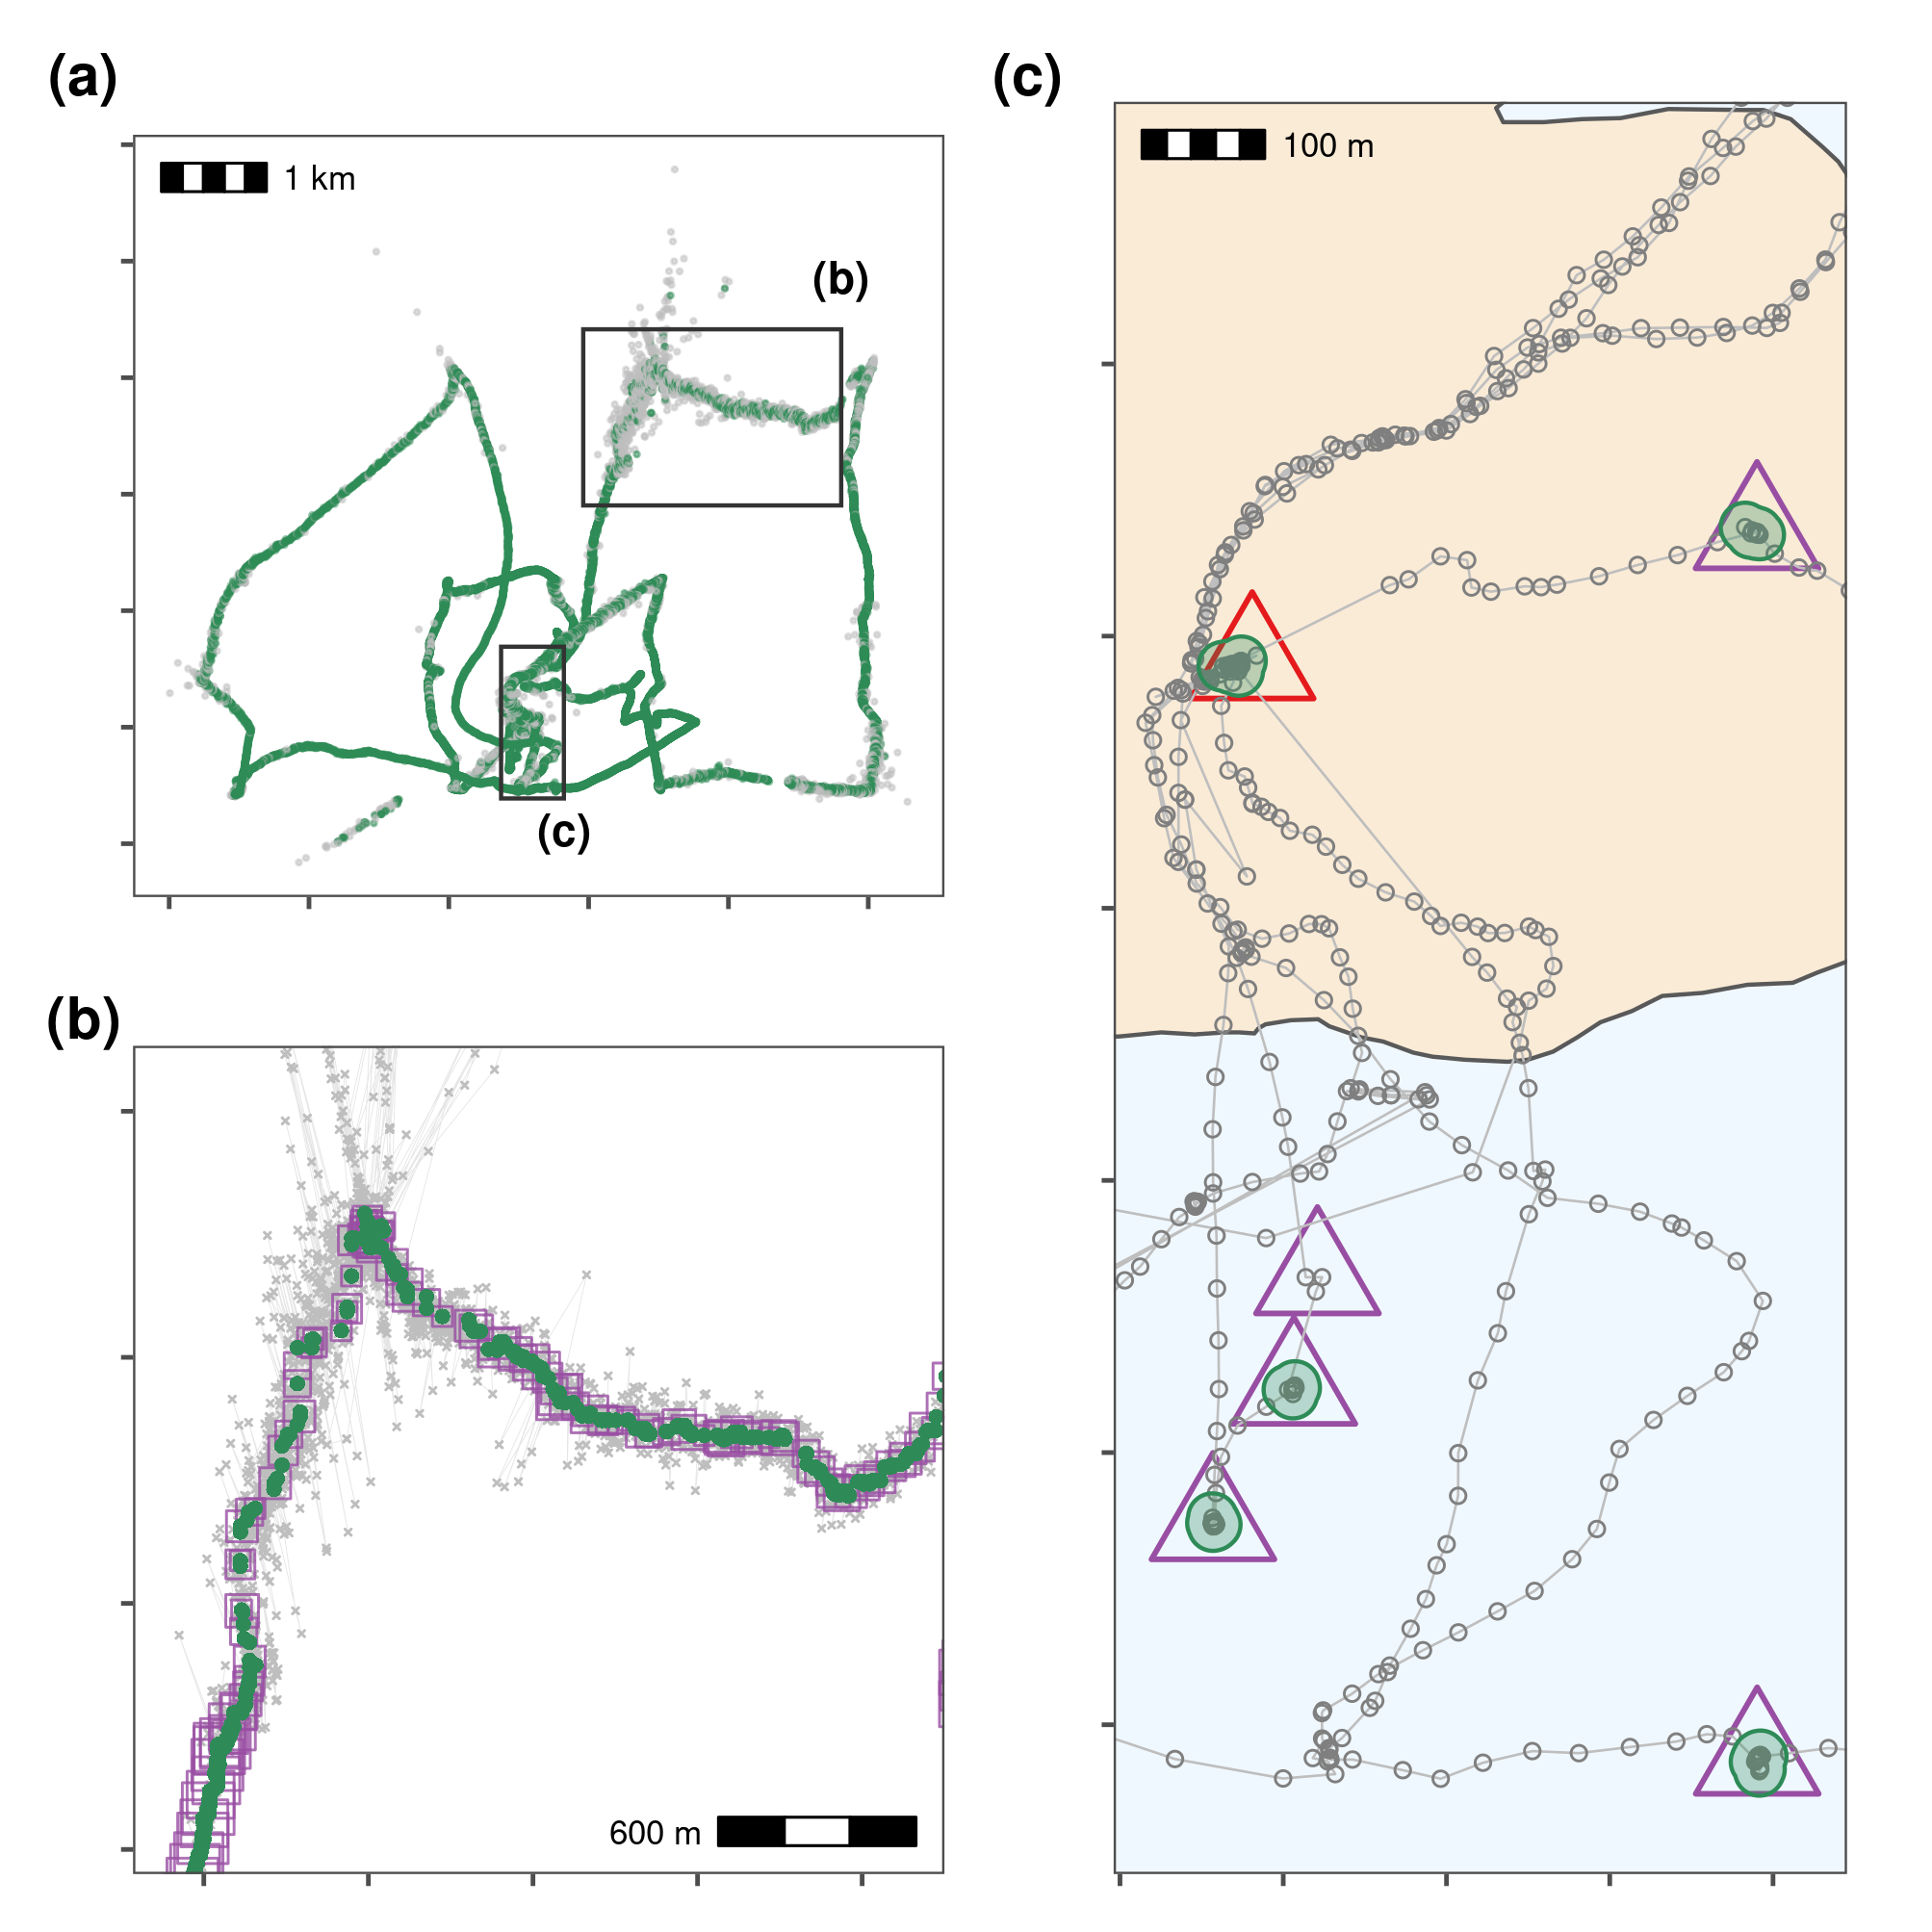
\includegraphics[width=0.75\textwidth]{figures/preprocessing/fig_07.png}
    \caption{
        \textbf{Pre-processing steps for WATLAS calibration data showing filtering on speed, median smoothing and thinning by aggregation, and making residence patches.}
        \textbf{(a)} Positions with incoming and outgoing speed $>$ 15 m/s are removed (grey crosses = removed, green points = retained).
        \textbf{(b)} Raw data (grey crosses), median smoothed positions (green circles; moving window $K$ = 5), and the smoothed track thinned by aggregation to a 30 second interval (purple squares).
        Square size corresponds to the number of positions used to calculate the averaged position during thinning.
        \textbf{(c)} Clustering thinned data into residence patches (green polygons) yields robust estimates of the location of known stops (purple triangles).
        The algorithm identified all areas with prolonged residence, including those which we had not intended to be recorded, such as stops at the field station (n = 12; red triangle).
        Our analysis could not find two stops of 105 and 563 seconds duration (6 and 15 fixes, respectively), since these were lost in the data thinning step; one of these is shown here (purple triangle without green polygon).
    }
    \label{preproc_fig_07}
\end{figure}

\section*{A Worked-Out Example on Animal Tracking Data}

We present a fully worked-out example of our pre-processing pipeline and residence patch method using movement data from three Egyptian fruit bats (\textit{Rousettus aegyptiacus}) tracked using the ATLAS system in the Hula Valley, Israel (33.1$^{\circ}$N, 35.6$^{\circ}$E) (\citealt{toledo2020, lourie2021}).
Code and data can be found in the Supplementary Material and Zenodo repository (see \textit{Processing Egyptian Fruit Bat Tracks}). 
Data selected for this example were collected over three nights (5\textsuperscript{th} -- 7\textsuperscript{th} May, 2018), with an average of 13,370 positions (SD = 2,173; range = 11,195 -- 15,542; interval = 8 seconds) per individual.
Plotting the tracks revealed potential location errors (see Fig.~\ref{preproc_fig_01}, see also Supplementary Material Fig.2.1), which we filtered out by removing observations with ATLAS SD $>$ 20 (see Supplementary Material Section 2.5), as well as removing observations calculated using fewer than four base stations, altogether trimming 22\% of the raw data (mean positions remaining = 10,447 per individual).
% We converted the ATLAS time format (milliseconds since the UNIX Epoch) to the more common UNIX format (seconds since the Epoch) by taking the floored value of the time divided by 1000.
Then, we removed unrealistic movement represented by positions with incoming and outgoing speeds $>$ 20 m/s that exceed the maximum flight speed recorded in this species (15 m/s; \citealt{tsoar2011}), leaving 10,337 positions per individual on average (98\% of previous step).
We median smoothed the data with a moving window $K$ size = 5, and no observations were lost.

We aimed to study bats' night-time foraging on fruit trees by quantifying the duration of bats' residence patches.
We began the construction of residence patches by finding the residence time within 50 metres of each position; this is the maximal radius of a `cloud of points' around fruit trees \citep{bracis2018}.
Foraging bats repeatedly traverse the same routes (\citealt{toledo2020, tsoar2011, lourie2021}) and this could artificially inflate the residence time of positions along these routes.
To avoid confusing revisits with residence, we limited the summation of residence times at each position to the period until the first departure of 5 minutes or more.
Thus, two nearby locations ($\leq$ 50m apart) each visited for one minute at a time, but separated by an interval of some hours would not be clustered together as a residence patch. 
To focus on bats' night-time foraging behaviour, we also excluded positions during the day (5 AM -- 8 PM), and at or near the roost-cave (see Fig.~\ref{preproc_fig_08}a) to focus on night-time foraging behaviour; 22,910 of 31,012 positions remained (73.9\%).
Since bats departed and returned to their roost at different times each night, we also excluded locations with a residence time $>$ 200 minutes (approx. 3.3 hours), as this was more likely to represent daytime roosting than nighttime foraging; of 31,012 smoothed positions, 18,677 remained (60\%).
From these positions, we calculated that between leaving the roost to forage, and returning, bats had a mean residence time at each position of 95.64 minutes (SD = 119.23) --- this value is still likely to be biased by some positions at the roost.

To determine the true duration of foraging, we opted for a first-principles approach and first selected only locations with a residence time $>$ 5 minutes, reasoning that a flying animal stopping for $>$ 5 minutes at a location should plausibly indicate resource use or another interesting localised behaviour.
This step retained 5,736 positions per bat on average (17,208 total), or 72.4\% of the nighttime positions.
We then constructed residence patches with a buffer distance of 25m, a spatial independence limit of 100m, a temporal independence limit of 30 minutes, and rejected patches with fewer than three positions.
These values are meant as examples; users should determine the sensitivity of their results to parameter choices.
Bats spent 56.95 minutes at foraging sites (SD = 62.20), and were stationary in particular fruit trees and roosting trees during 83.8\% of their foraging time (Fig.~\ref{preproc_fig_08}).
Although all three bats roosted at the same cave during the day, and all their tracks are within the typical foraging area of bats roosting in this cave \citep{lourie2021}, they used distinct foraging sites across the area at night (Fig.~\ref{preproc_fig_08}.a). The lack of overlap among individuals in tree use, obtained with the residence patch algorithm, shows that although co-roosting bats share the same cave-specific foraging area \citep{lourie2021}, they often forage on different trees.
Contrasting the actual movement path with the linear path between residence patches can help reveal details of how animal cognition affects space use \citep{toledo2020}.
Bats tended to show prolonged residence near known food sources (fruit trees), but also where no fruit trees were recorded (Fig.~\ref{preproc_fig_08}.b, ~\ref{preproc_fig_08}.c), in line with previous evidence for their use of non-fruiting trees to rest, to handle and digest food, and presumably for social interactions \citep{tsoar2011}.

\begin{figure}[h!]
    \centering
    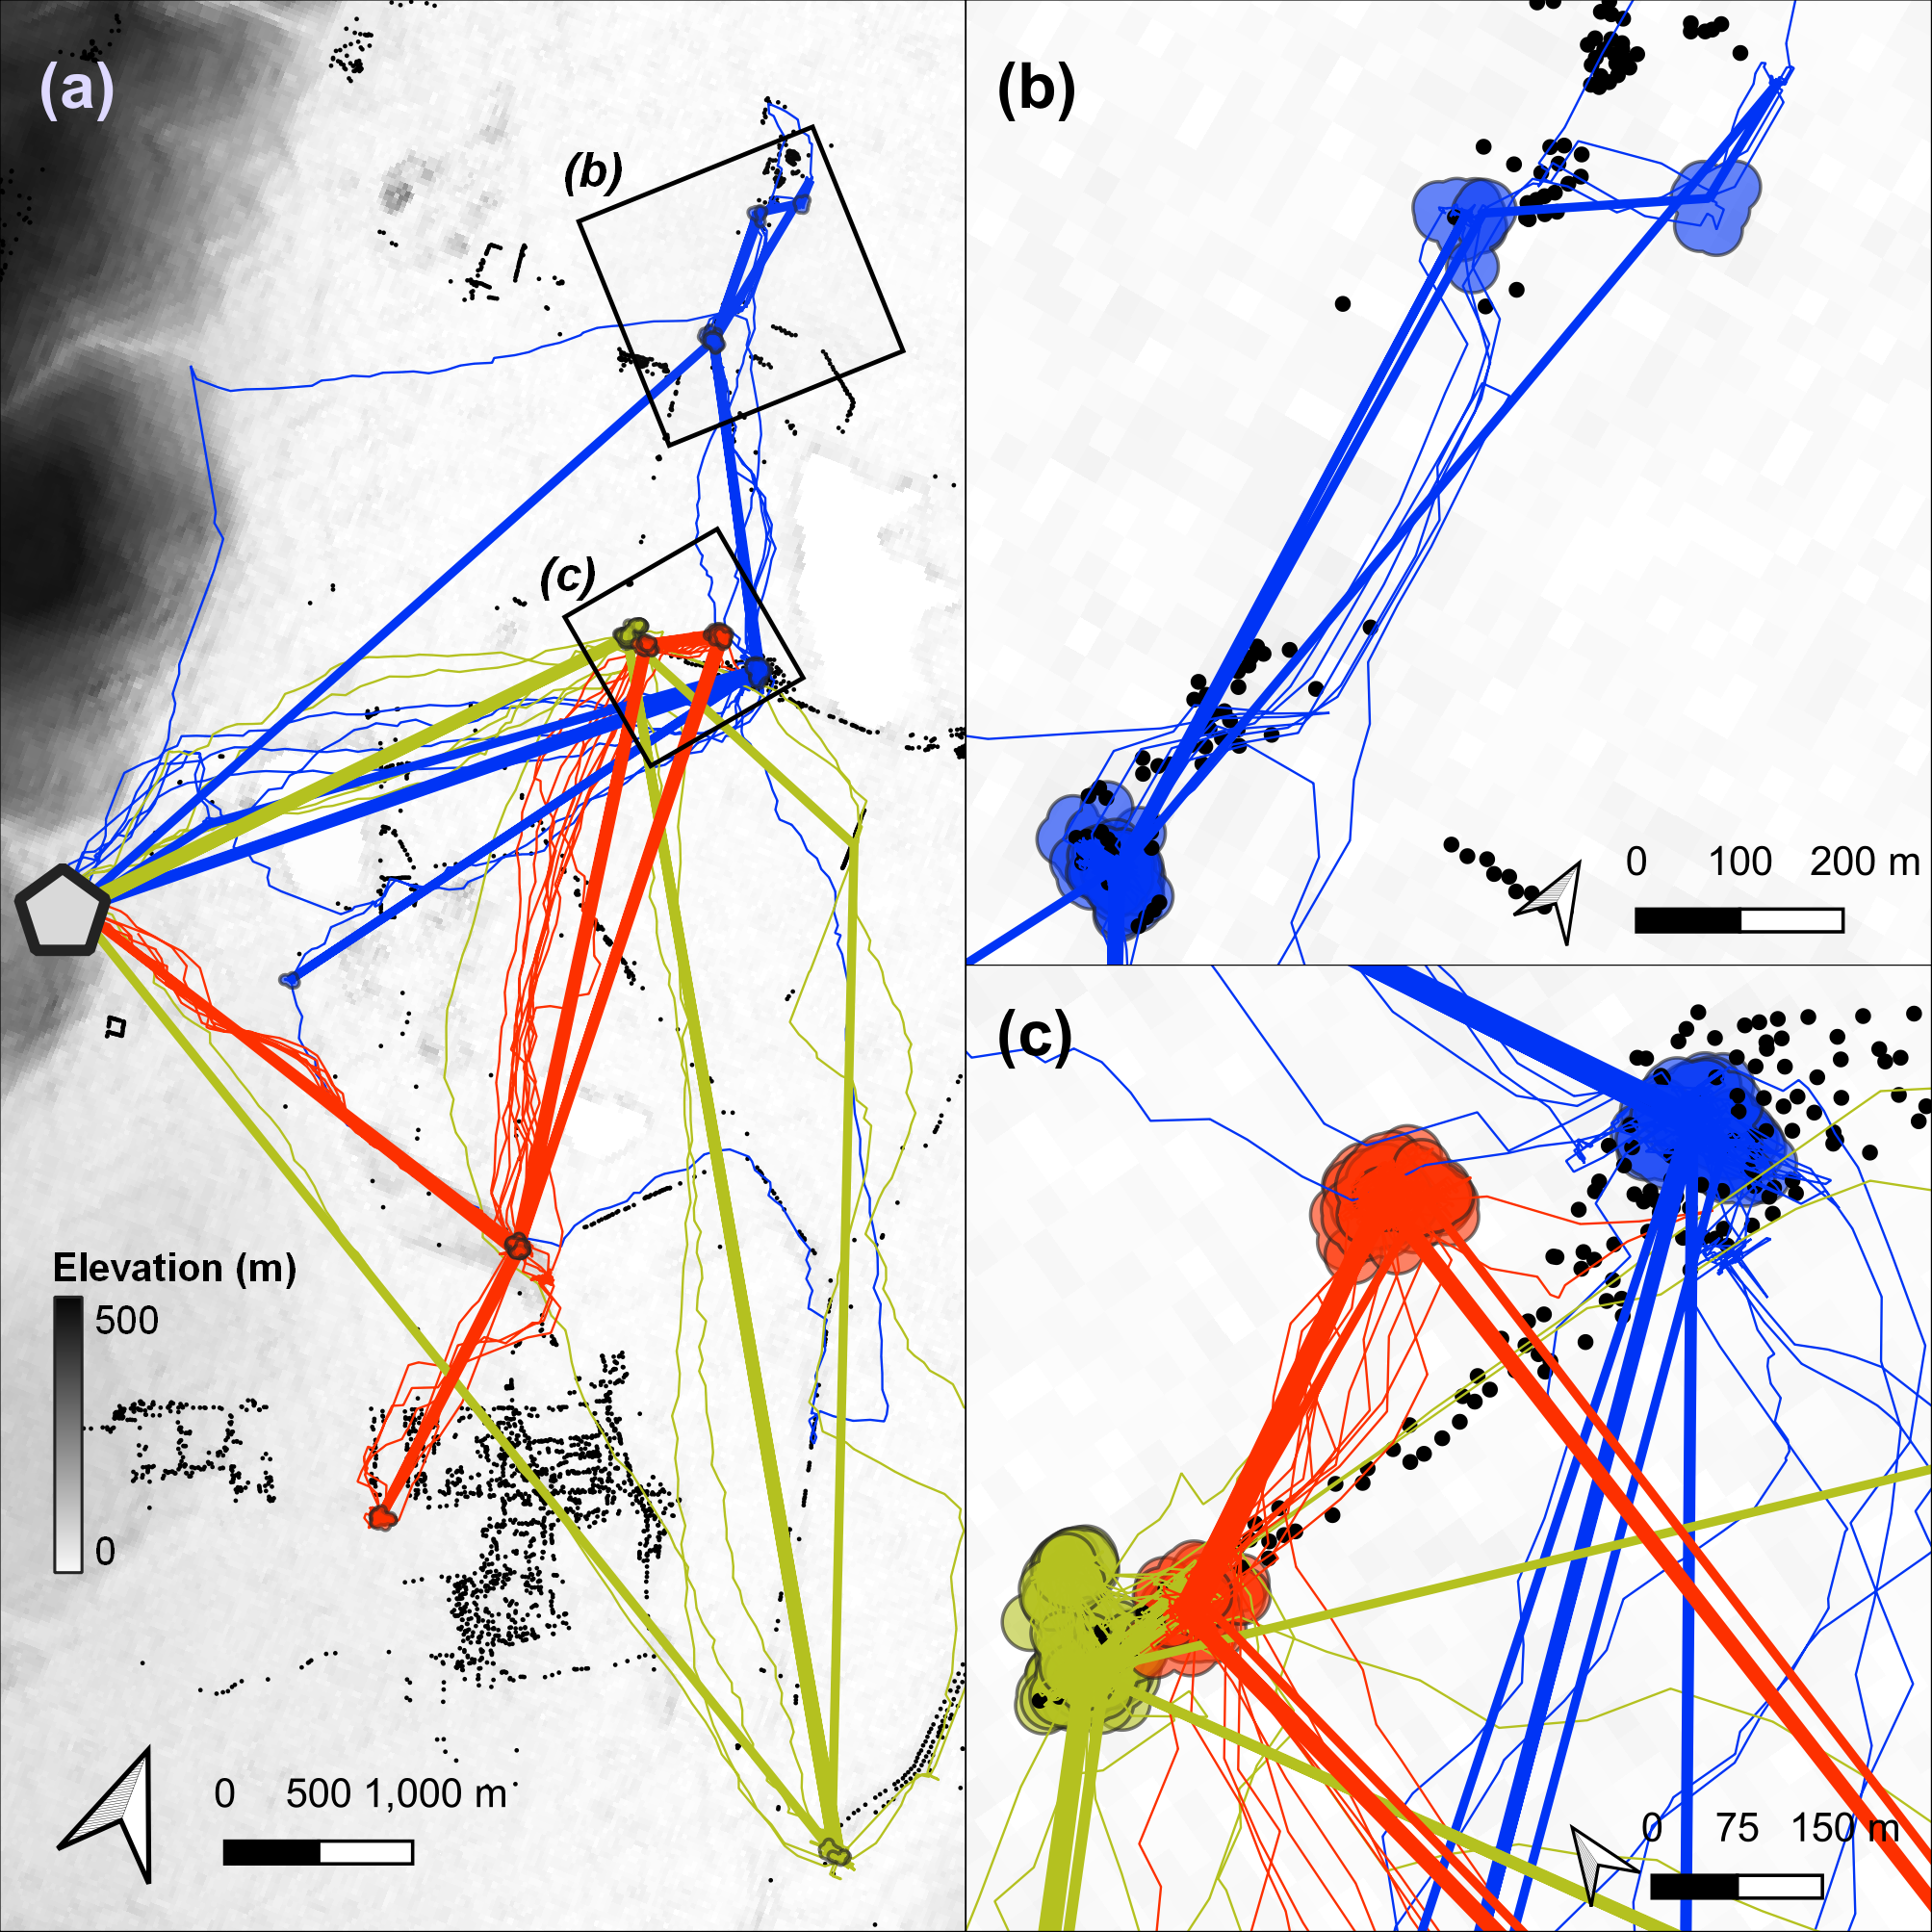
\includegraphics[width=0.75\textwidth]{figures/preprocessing/fig_08.png}
    \caption{
        \textbf{Synthesising animal tracks into residence patches can reveal movement in relation to landscape features, prior exploration, and other individuals.}
        \textbf{(a)} Linear approximations of the paths (coloured straight lines) between residence patches (circles) of three Egyptian fruit bats (\textit{Rousettus aegyptiacus}), tracked over three nights in the Hula Valley, Israel.
        Real bat tracks are are shown as thin lines below the linear approximations, and colours show bat identity. The grey hexagon represents the roost-cave at Gar Hershom.
        Black points represent known fruit trees.
        Background is shaded by elevation at 30 metre resolution.
        \textbf{(b)} Spatial representations of an individual bat's residence patches (green polygons) can be used to study site-fidelity by examining overlaps between patches, or to study resource selection by inspecting overlaps with known resources such as fruit trees (black circles).
        In addition, the linear approximation of movement between patches (straight green lines) can be contrasted with the estimated real path between patches (irregular green lines), for instance, to determine the efficiency of movement between residence patches.
        \textbf{(c)} Fine-scale tracks (thin coloured lines), large-scale movement (thick lines), residence patch polygons, and fruit tree locations show how high-throughput data can be used to study movement across scales.
        Patches and lines are coloured by bat identity.
    }
    \label{preproc_fig_08}
\end{figure}

\section*{Future Perspectives on Pre-processing Tracking Data}

Recent technical advances in wildlife tracking have already yielded exciting new insights from massive high-resolution movement datasets \citep{aspillaga2021, aspillaga2021a, baktoft2017, baktoft2019, harel2016, harel2018, oudman2018, papageorgiou2019, tsoar2011, strandburg-peshkin2015, toledo2020, beardsworth2021a, beardsworth2021b, corl2020, vilk2021, lourie2021}, and high-throughput animal tracking is expected to become increasingly more common in the near future.
Tackling the very large datasets that high-throughput tracking generates requires a different approach from that used for traditionally smaller volumes of data.
We foresee that movement ecologists will have to adopt ever more practices from fields accustomed to dealing with `big data', and that the field will become increasingly computational \citep{peng2011}.

Researchers have long used some of these approaches \textit{ad hoc}, such as exploratory data analysis on small subsets before applying methods to the full data, using efficient tools, and basic batch-processing. 
Yet formally prescribing these steps can help practitioners avoid pitfalls and implement techniques that make their analyses quicker and more reliable.
Standardised principles, implemented a basic pipeline, for approaching data cleaning promote reproducibility across studies, making comparative inferences more robust.
While massive datasets make reliance on standardised pipelines necessary, the output of such pipeline should periodically manually double-checked to ensure `realistic' output.
The open-source \textit{R} package \textit{atlastools} serves as a starting point for methodological collaboration among movement ecologists, and as a simple working example on which researchers may wish to model their own tools.
Efficient location error modelling approaches \citep{fleming2020, aspillaga2021} may eventually make data-cleaning optional.
Yet cleaning tracking data even partially before modelling location error is faster than error-modelling on the full data, and the removal of large location errors may improve model fits.
Thus we see our pipeline as complementary to these approaches \citep{fleming2014, fleming2020}.

Finally, we recognise that the diversity and complexity of animal movement and data collection techniques often requires system-specific, even bespoke, pre-processing solutions.
Though the principles outlined here are readily generalised to numerous data sources (including terrestrial radio-based reverse-GPS: e.g. \citealt{toledo2020}, and marine acoustic reverse-GPS: e.g. \citealt{aspillaga2021}; high-resolution GPS such as \citealt{strandburg-peshkin2015}, and video-tracking: \citealt{rathore2020}), users' requirements will eventually exceed the particular tools we provide.
For instance, relational databases are the standard for storing very large datasets, and extending pre-processing pipelines to deal with various data sources is relatively simple, as we show in our Supplementary Material.
We see the diversity of animal tracking datasets and studies as an incentive for more users to be involved in developing methods for their systems.
We offer our approach to large tracking datasets, and our pipeline and package as a foundation for system-specific tools in the belief that simple, robust concepts are key to methods development that balances system-specificity and broad applicability.\\
{ \begin{center} \barfont{-.-} \end{center} }

%%%%%%%%%%%%% Supplement %%%%%%%%%%%%%%%

% \newpage

\begingroup

\let\clearpage\relax
\let\cleardoublepage\relax
\let\cleardoublepage\relax

{\chapter*{Supplementary Information for Chapter~\ref{ch:preprocessing}}}

The supplementary material for this chapter is a worked out, step-by-step guide to using the \emph{atlastools} package to clean data as described in preceding sections.
Being primarily a tutorial for practitioners --- and quite lengthy --- it is not provided here, but may be found online as Supporting Information published along with the manuscript, \textcite{gupte2022d}, \citetitle{gupte2022d}, at:
https://besjournals.onlinelibrary.wiley.com/doi/10.1111/1365-2656.13610.

{ \begin{center} \barfont{-.-} \end{center} }

\endgroup

%     \newrefcontext[sorting=nyt]
%     \section*{Literature Cited}
%     \printbibliography[title=Literature~Cited,heading=none]
% \end{refsection}


\clearpage \cleardoublepage
\begin{interludeenv}

% \addtocontents{toc}{\protect\vspace{\beforebibskip}}%
%\chapter*{Mapping Animal Movement in \textit{R}: The Science and the Art}
%\chaptermark{Mapping Animal Movement in \textit{R}: The Science and the Art}
\phantomsection
\pagestyle{plain}
\pagecolor{Snow2}
% \begin{addmargin}[-2.0cm]{0cm}

	\addcontentsline{toc}{chapter}{\tocEntry{\color{gray}\bfseries{Box 1: Mapping Animal Movement in \textit{R}}}}%
	\medskip
	\section*{Box 1: Mapping Animal Movement in \textit{R}}\label{box:mapping}
	\chaptermark{Mapping Animal Movement in \textit{R}}

	In December 2020 I was pointed to the BES Mapping Animal Movements Contest, and the “R Map” category stood out to me. I entered a map made showing the movement of 14 savanna elephants \textit{Loxodonta africana} tagged in Kruger National Park, South Africa.

	\graffito{
		{\large{$\Delta$}} This box is adapted from a submission to the Methods in Ecology and Evolution blog, after my entry won the BES' Mapping Animal Movements Contest.

		The study that inspired this map was published as \cite{thaker2019}.
	}

	The map highlights the path of the female elephant AM253 (the tag number). Some of the thirteen other elephants are also shown to give a sense of how densely Kruger is criss-crossed by elephant herds. The background shows the average temperature sensed by the LANDSAT-5 satellite over the two year period of this study.

	This data was part of the postdocs of Maria Thaker and Abi Vanak, for whom I worked between my master's and my PhD. We wrote a paper about how Kruger elephants move in response to temperature. The source code and the map I made can be found here.

	\paragraph*{Mapping as Exploratory Data Analysis}

	Mapping animal movements is a key component of exploratory data analysis. It's important for `joining the dots' of animal positions. Large tracking datasets can contain errors that are only evident to researchers when they look at an approximation of the animal's path and ask, “Does the animal move this way?”

	For instance, this map shows `jumps': long, linear segments between points, which indicate missing data for some periods. Mapping can also reveal interesting behaviours that can only be observed after significant effort in the field.

	For instance, the `looping' behaviour of AM253 to water sources is the focus of this map. Seeing this looping behaviour allowed us to focus our study on elephant movements between visits to water sources.

	\paragraph*{Mapping as Art}

	As with many other areas of science (other than primary data collection), when in doubt about maps, copy.

	Growing up in early 2000s India, I read hard copies of National Geographic Magazine, which has long had fantastic graphics. Where the Animals Go was a source of inspiration as well. I picked up other tips and tricks from knowing something of art generally: build up an image in layers, use colours that don't clash, highlight the phenomenon of interest. Interestingly, some of these approaches are very much in line with the `grammar of graphics' approach of \textit{ggplot}, which I used to make this map.

	\paragraph*{Mapping in R}

	I used LANDSAT-5 for the temperature layer because it was the appropriate satellite for the time period (2007), and had a decent spatial resolution (30 metres). I used Google Earth Engine (GEE) to acquire this data. The heavy computation happens on the GEE servers, significantly increasing speed. By collecting these data for use at one point, GEE also improves data accessibility.

	I used Python to get the LANDSAT-5 data from Google Earth Engine, using the ee package, which is the Python GEE API package. The \textit{rgee} R package is similar, but works via Python, so I used Python directly.

	I found Qiusheng Wu's \textit{geemap} package a great tool for visualisation of the data I was working with, and the associated tutorials a very good resource for help with ee generally.

	\paragraph*{Getting Elephants and Other Landscape Features}

	In 2019, we published the data on the Movebank data repository (It now forms part of the animation on the starting page). Getting the data was thus very easy using the move package, which I then saved as a \textit{geopackage}.

	I acquired the river course data using the \textit{osmdata} package, which queries and retrieves data from the \textit{OpenStreetMap} database. The boundaries of Africa and South Africa come from the \textit{rnaturalearth} package. The Kruger boundary and the locations of waterholes originally come from the South African National Park service.

	\paragraph*{Choosing Mapping Tools}

	R's great advantage over other languages is visualisaton, specifically the popular ggplot package. \textit{ggplot}'s emergence as a mainstay of spatial visualisation is due to its \textit{geom\_sf} function, which can handle sf spatial objects.
	
	One of ggplot's advantage's is its many extensions. Here, I used the ggspatial and ggtext extension packages to add the scale bars and north arrow, and to add the text box, respectively.
	
	Plotting rasters is not straightforward in ggplot. There are two main options: the stars package and its associated \textit{geom\_stars}, or converting a raster dataset into a dataframe with regular coordinate intervals and using \textit{geom\_tile}.
	
	Here, I chose the second approach because I'm an infrequent stars user; since making the map I've tried \textit{geom\_stars} which works just as well, and is very convenient.

	\paragraph*{Choosing Map Colours}

	I coloured the temperature raster using the \textit{scico} package's `VikO' palette. I tried out a number of palettes from \textit{scico}, pals (providing the Kovesi palettes), \textit{RColorBrewer}, and \textit{colorspace} packages. I chose a diverging palette to show heterogeneity in the thermal landscape, but this approach is not to be recommended for material that will be printed in grayscale.

	\paragraph*{Reproducibility in R}

	I adopted a relatively relaxed understanding of reproducibility: given the data, the code would be reproducible if it could produce the map I had entered for this contest. To do this, I set up a continuous integration pipeline using Github Actions (GHA).

	Using the \textit{usethis} package, I created a DESCRIPTION file, which is usually reserved for packages. This file tricks GHA into reading its contents, especially the dependencies, i.e., the R packages required by the project.

	GHA automatically reads the dependencies and installs them, as well as the programs required by those dependencies. For instance, GDAL (the Geospatial Data Abstraction Library) is key to nearly all spatial analyses, and is installed as a requirement of the \textit{rgdal} package, which is itself key to \textit{sf} and \textit{raster}.

	I used the R package \textit{renv} to make sure that the packages (and the package versions) I used are available to the pipeline. \textit{renv} creates a lockfile, a registry of packages the current project uses, from which those packages can be installed.

	Finally, to check whether the entire pipeline works, I used \textit{bookdown} to sequentially execute the series of Rmarkdown files. An obvious alternative is \textit{rmarkdown}.

	GHA runs this pipeline and reports whether the code ran successfully, and if not, where it failed (you can see these reports here). GHA runs the pipeline on Linux, and Windows containers (Mac OS-x is also supported). This means that though I use Linux, I'm pretty sure that this code works for Windows users.

	\paragraph*{The Limits of Reproducibility}

	Reproducibility inevitably breaks down at certain scales in an ecological study. For instance, it would be impossible to reproduce the primary data collection of the study, such as which elephants were captured and fitted with transmitters. These data are taken on faith from the original researchers, highlighting the role of trust in the scientific community.

	Code too is not exempt from reproducibility limits. For instance, restoring the \textit{renv} lockfile is very difficult without an internet connection, as packages may need to be downloaded.

	In ten years, code in R or another language may no longer be reproducible due to software and hardware changes, as many researchers found in the 10-year reproducibility challenge. Finally, entire services might become unavailable; for example, the raster processing using Google Earth Engine is dependent on Google maintaining this service.

	Researchers then, should be pragmatic about reproducibility. Who is it for — the researchers themselves, the reviewers of their manuscript, their students, their funders?

	To whom is this effort owed, and by whom, and how can the additional work required be prevented from becoming a gatekeeping mechanism {\color{red}(1), (2)}? These are issues that the ecology and evolution community will have to address.
	
% \end{addmargin}
\afterpage{\nopagecolor}
\pagestyle{scrheadings}

\end{interludeenv}

\cleardoublepage %************************************************
\chapter{Direct Effects of Wing Moult on the Movement and Habitat Selection of Sub-tropical Birds}\label{ch:holeybirds}
\chaptermark{Wing Moult \& Movement}
%************************************************

{\noindent \sffamily\textbf{Pratik R. Gupte}, Yosef Kiat\textsuperscript{1}, Sivan Toledo\textsuperscript{2}, and Ran Nathan\textsuperscript{3}}

\marginpar{
    \sffamily
    \textsuperscript{1} University of Haifa, Israel.
    
    \medskip
    
    \textsuperscript{2} Tel Aviv University, Israel.
    
    \medskip

    \textsuperscript{3} The Hebrew University of Jerusalem, Israel.
}

\section*{Abstract}

% \marginpar{ 
%     \bigskip

%     {\large{\color{Maroon}$\Delta$}} \normalfont Published in the \textit{Journal of Animal Ecology} as Gupte et al. (2021). A guide to pre-processing high throughput tracking data.
% }

\small{
    The feathered flight of birds requires regular renewal of the wing surface through moult, the process of shedding worn out feathers and growing fresh ones.
    Moult presents birds with the dilemma of needing to move more to acquire resources for feather growth, at precisely the time that their flight capacity is reduced (due to missing wing feathers) and they are vulnerable to predation.
    Despite this central importance of moult to avian ecology, and especially to movement, we know little about its direct effects on the spatial ecology of birds.
    We combined a range of mechanistic approaches to present a first quantification of the direct, short-term effects of wing moult on the movement and habitat selection of four different non-migratory, sub-tropical birds.
    We quantified landscape visibility from a predator viewpoint, and followed the movement of birds in different stages of moult, with a high-throughput position tracking system.
    We found that birds balanced the needs and risks of moult by adjusting their movement to their wing condition.
    Naturally moulting birds moved more than non-moulting birds, but birds with wing feathers experimentally removed moved less.
    Among similarly vegetated areas, birds preferred low-visibility sheltered sites in our agricultural landscape, regardless of their moult status.
    Intriguingly, our results suggest that birds' cognitive abilities may extend to seeing a landscape from the spatial perspective of another individual.   
}

\clearpage



\begin{refsection}

\newrefcontext[sorting=ynt]

\lettrine{B}{irds} are unique in moving mostly by powered flight on feathered wings.
Feathers, unlike animal hair and claws, are dead proteinaceous structures, which cannot be renewed continuously as they suffer wear and tear \cite{rayner1988,jenni1989}.
As feathers mature, wing condition and consequently flight capacity gradually decreases \cite{lindstrom1994,hedenstrom1999,hedenstrom2003}.
Molt --- the shedding of old, worn-out feathers, and their replacement with freshly grown ones --- is thus a key process in avian ecology \cite{ginn1983,rayner1988}.
During wing molt, as one or more feathers are lost and new ones grow in their place, the flight surfaces of bird wings become smaller.
The reduction in flight surface area during molt can be measured using a robust-cross species index of the size of the (temporary) wing gap \citep{lind2001,kiat2016}.
Wider gaps lead to larger reductions in flight surface area, power output, and flight capacity and efficiency in captive birds \cite{tucker1991,swaddle1996,swaddle1997,williams2003,lind2001,lind2001a,bowlin2009}.
In addition to these indirect costs, wing molt is among the most energetically demanding phases of a bird's annual cycle, as regrowing large flight feathers requires substantial resources \cite{lindstrom1993,newton2009,kiat2017}.
Despite these mechanistic links between molt and movement, our understanding of molt's influence on birds' movement strategies and habitat selection is poor.

The direct influence of wing molt on the movement and habitat selection of birds has primarily been examined in a few small-scale, disconnected studies \citep{bell1970,haukioja1971,green1975,francis1991,madsen1987a,fox1998}.
Moving less, as some northerly species of finches and buntings do \citep{bell1970,haukioja1971,green1975,francis1991}, could save energy required to regrow feathers.
Avoiding predation risk during molt by sheltering in vegetation and rough terrain \citep{bell1970,haukioja1971,green1975,francis1991}, or near water-bodies as geese and ducks do \cite{madsen1987a,fox1998}, could also lead to reduced movement during molt.
Molt often coincides with migratory periods \citep{kiat2019}, making it difficult to separate the effects of migration-related energetic requirements \cite{alerstam1990,wikelski2003,horvitz2014}, such as preferences for high-quality resources \cite{madsen1987a,fox1998}, from molt-related considerations on habitat selection.
Simultaneously, molt is influenced by bird physiology, with large-bodied species molting faster \citep{kiat2021,jenni2020}, and also by birds' evolved movement strategies, as wide-ranging and aerial foraging species (e.g., swifts and swallows) molt more slowly to maintain movement capacity \cite{kiat2016}.

The direct effects of molt could be robustly studied with a cross-species comparison of unrelated, non-migratory species that are not constrained by the short time available for molt in northern temperate regions \cite{ginn1983,jenni2020}.
Cross-species studies of movement and habitat selection in molting birds could benefit from dramatic advances in the high-throughput position tracking of small species \cite{toledo2020,nathan2022}.
Birds, among other animals, can take the spatial perspective of visual predators, and avoid risky, exposed areas in favour of sheltered ones \cite{hampton1994,emery2000,krams2001,davidson2016,krams2020}.
Shelter is often only proxied by correlated variables, such as vegetation growth \cite{pettorelli2011}. 
Adopting a mechanistic, viewshed ecology approach \cite{olsoy2015,aben2018,aben2021} in habitat selection analyses could directly account for birds' visibility to potential predators \cite{olsoy2015,aben2018,aben2021}.

We explore the direct effects of wing molt on the movement of birds, focusing on four sympatric, non-migratory species: barn swallows (\textit{Hirundo rustica}), white-spectacled bulbuls (\textit{Pycnonotus xanthopygos}), house sparrows (\textit{Passer domesticus}), and clamorous reed-warblers (\textit{Acrocephalus stentoreus}).
Scoring the molt-related wing gap size of naturally molting birds \citep{lind2001,kiat2016}, we manipulated a subset of molting individuals by trimming a number of flight feathers.
We tracked birds during a 4-month period using the high-throughput ATLAS system, which brings unprecedented temporal and spatial resolution to small bird tracking \citep{toledo2014,weiser2016,toledo2020,nathan2022,beardsworth}.
We examined \textit{(i)} how the size of the molt-related wing gap affected bird movement, and \textit{(ii)} how the wing gap size influenced selection for more sheltered habitats.
Overall, we show how birds' movement decisions, influenced by their immediate physiological condition, scale up to affect their space use, and how individuals' adaptive behavioral strategies have feedbacks with their evolutionary ecology.

\section*{Methods}

We studied bird molt and movement in the Hula Valley of northern Israel (33.10°N, 35.60°E), which includes reconstructed wetlands and reedbeds as well as agricultural areas (crops, plantations and fishponds; see \textit{SI Appendix}).

\subsection{Bird capture, wing molt scoring and experimental manipulation}

We captured 86 individuals of four species in 2016: 16 barn swallows, 19 white-spectacled bulbuls, 35 house sparrows, and 16 clamorous reed-warblers, for which we also measured the wing gap index.
All individuals were trapped after breeding was completed and before the molting season commenced, between June and October 2016.

We described the state of each primary feather on a scale of 0 to 5 using the primary score (PS) method \citep{ginn1983}.
Both PS = 0 and PS = 5 indicate a fully mature feather, and hence no gap in the wing.
A PS value between 1 and 4 indicates feathers in increasing stages of growth, with PS = 1 representing a large gap left by a recently molted feather.
This method allows a cross-species estimate of the size of the molt-related gap in the wing, and is also strongly and negatively correlated with molt rate and duration \citep{rohwer2009}.
We scored the wing gap size due to any single feather molting as the inverse value of PS for each of the wing's nine primary feathers (P1 -- P9; counted outward) such that when PS = 1, wing gap size = 4, and when PS = 2, wing gap size = 3, etc.
However, for PS = 0, wing gap size is also 0 because there is no gap in both the PS = 0 and PS = 5 stages, as either an old, mature feather, or a new, freshly grown feather is present.
To compare molt-related wing gap sizes across individual birds, we summed the wing gap size scores across all nine primary flight feathers, for each individual, into a single wing gap index \citep{kiat2016}.
This index is independent of the size of individual birds and their morphology, controls for the stage of wing feather molt, and allows for reliable cross-species comparisons \citep{bensch1993,kiat2016}.

We experimentally manipulated 29 individuals across species {(bulbuls = 6, sparrows = 14, reed-warblers = 2, swallows = 7)}, and removed one to three primaries; the exact number was determined randomly for each bird.
We varied this number to produce variation in the possible effect of wing gap size, and the manipulation was symmetrical, i.e., the same feather was removed in both wings.
Primaries were removed by cutting the feather near its base, in addition to the primaries missing as part of natural molt; this procedure simulates an enlargement of the molt-related wing gap.
Cutting the feather rather than tearing it out from the base, which is still innervated \cite{jenni2020}, avoided excess trauma which could impact birds' behaviour, and allowed us to examine the effect of only the wing gap size on movement and habitat selection.
For these experimentally manipulated birds, we calculated the wing gap size after the procedure described here.
Bird capture and handling, the experimental manipulation procedure, and tagging for position tracking (see below) were conducted under a permit from the Israel Nature and Parks Authority (NPA permit 2016/41402) and from the ethics committee of the Hebrew University of Jerusalem, Israel (NS-16-14801-2).

\subsection{Forecasting daily changes in the wing gap size index}

The size of the molt-related wing gap decreases slowly and constantly as feathers regrow, yet as a mature feather is shed, the wing gap size may also increase in gradual jumps.
Over our tracking period of about 7 days per individual (see below), this is expected to represent small changes in the wing surface area, which could further influence movement decisions.
These changes in wing condition should be accounted for when relating movement characteristics to wing gap size.
To do this, we calculated for each species the mean daily progress in the molt score, based on a sample of individuals documented twice during the molt process (bulbul = 0.45 $\pm$ 0.15, n = 17; sparrow = 0.40 $\pm$ 0.25, n = 10; reed-warbler = 0.69 $\pm$ 0.34, n = 24; swallow = 0.34 $\pm$ 0.18, n = 22). 
Then, we estimated for each bird included in the study the expected daily change based on the measurement we made at the time of tagging (see \textit{SI Appendix}).

\subsection{Tracking bird movement using ATLAS}

We tracked the movement of individual birds using ATLAS (Advanced Tracking and Localization of Animals in real-life Systems), a state-of-the-art high-throughput radio-telemetry system capable of tracking dozens of individuals at intervals as low as 4 seconds \citep{weiser2016,toledo2014,toledo2020,nathan2022}.
We glued ATLAS tags (0.9 -- 1.6 g, depending on species) to birds' dorsal feathers after capture, and then released them (tag weights as percent of body mass: bulbuls = 3.85\% $\pm$ 0.21\%; sparrows = 4.21 $\pm$ 0.13; reed-warblers = 4.75\% $\pm$ 0.19\%; swallows = 4.9\% $\pm$ 0.13\%).
Tags automatically drop off as these feathers are molted.
Each individual was tracked for an average of 8.23 $\pm$ 3.24 days (bulbul = 9.8 $\pm$ 10.1 days; sparrow = 12.0 $\pm$ 13.4 days; reed-warbler = 5.9 $\pm$ 2.1 days; swallow = 5.1 $\pm$ 14.8 days).
We collected 4.3 million position estimates overall, with 7,276 positions per individual per day, for an effective tracking interval of 5.05 $\pm$ 1.85 positions per minute on average (bulbuls = 6.14 $\pm$ 3.93; sparrows = 5.98 $\pm$ 5.57; reed warblers = 5.80 $\pm$ 3.16; swallows = 2.28 $\pm$ 1.42).
Since we were interested in exploring movement patterns, and these species are diurnally active, we removed all nighttime positions, leading to an approximate halving of the total dataset.

\subsection{Processing tracking data}

ATLAS conservatively filters out location estimates that are clearly wrong (e.g., too far from the study area), letting users inspect most location estimates, which come with several measures of quality, 
% (estimated covariance matrix, quality of fit to constraints, and the norm of the gradient of the objective function), 
and decide whether they want to retain the estimates or not. 
For this study, we aggressively filtered out location estimates, removing estimates for which we had indications that ATLAS failed to find a high-quality estimate \citep{gupte2022d} (see \emph{log\_preprocessing.log} in the analysis code).
We began data cleaning by removing locations near a so-called attractor position (at (257000.0,780000.0), Israeli grid; see file \textit{log\_preprocessing.log}); these are locations for which the positioning system had defaulted to a (wrong) estimate.
We identified and removed other attractor positions by removing positions sharing the exact same common coordinate pair. 
Since coordinates are resolved down to double-precision, it is very unlikely for two location estimates to have the same coordinate pair, and this rather indicates an error in location estimation.
Each individual's track was pre-processed separately.

We first \textit{(i)} filtered the data for large-scale errors by removing positions with a system-generated positioning-error estimate (SD) $>$ 20m, and then \textit{(ii)} split each individual's tracking data by calendar date, removing days with $<$ 500 positions. 
Finally, we \textit{(iii)} filtered the data for unrealistic movements, removing positions with both speeds $>$ 20 m/s \emph{and} a turning angle >10\textdegree.
We deliberately used larger thresholds than these species' maximum speeds to avoid removing valid, high-speed movements \citep{gupte2022d}.
Finally, we \textit{(iv)} accounted for small-scale errors --- noise around the true positions --- by applying a median smooth with a moving window $K$ = 7.
After excluding night time data and all other data filtering and smoothing, we analyzed 1.1 million locations from 86 individuals, keeping high per-minute sampling rate for all species (bulbuls = 4.85 $\pm$ 3.3, sparrows = 2.73 $\pm$ 3.0, reed-warblers = 2.09 $\pm$ 1.44, swallows = 2.07 $\pm$ 1.14).
Compared with current technologies for tracking small birds ($<$ 50g) --- primarily radio triangulation and geolocators, which have low temporal (a few fixes per hour or day) and spatial resolution (error margins up to 200 km) \citep{bridge2013} --- ATLAS data represent an unprecedented sampling rate, with GPS-level accuracy \citep{beardsworth}.

\subsection{Quantifying large-scale movements}

We investigated the large-scale space-use of bulbuls, sparrows, and reed-warblers by summarising their processed movement paths into daily sequences of `residence patches' using the \textit{atlastools} package developed specifically with high-throughput ATLAS tracking data in mind \citep{gupte2022d}.
The residence patch algorithm uses simple distance and duration thresholds, chosen based on the movement ecology of the tracked species, to efficiently and rapidly cluster-segment individuals' non-travelling positions \citep{gupte2022d}.
We applied this algorithm to the date-specific tracks of each individual, considering consecutive positions less than 25m and 30 minutes apart to be part of the same cluster.
We joined clusters (with at least 9 positions) less than 100m and 30 minutes apart together for bulbuls and sparrows, and less than 25m and 30 minutes apart for reed warblers, which typically fly only short distances \cite{kiat2016}.
Doing so, we obtained 4,373 residence patches overall and extracted environmental covariates (NDVI and visibility index; see below) for the positions clustered into each patch.
%%
We handled swallows differently, as these are highly aerial birds whose movement is not easily clustered into residence patches.
Instead, and because the relatively higher-flying swallows are more accurately tracked by ATLAS, we simply calculated the total distances moved along daily tracks from the cleaned, processed data.

\subsection{Visibility analysis to quantify sheltered habitats}

Many animals can gauge the risk posed by predators by estimating a predator's field of view (`spatial perspective taking') \cite{emery2000,bruce2003,davidson2016}, and select for sheltered locations outside of a predator's view \citep{hampton1994,krams2001,watve2002}.
To assess the field of view of a hypothetical predator, and thus the estimated riskiness of the landscape, we took a viewshed ecology approach to determine how visible an area was from surrounding locations \citep{aben2018,aben2021}.

We first obtained a 50cm canopy height model (CHM) \citep{aben2021} of the majority of our study area (courtesy of the Survey of Israel).
For each cell of the CHM, we calculated a \textit{visibility index}, which is the proportion of surrounding cells from which the focal cell is visible, given that lines of sight can be blocked by intervening structures (also called cumulative viewshed analysis, or a `fearscape') \cite{olsoy2015}.
Open areas, such as agricultural fields or water bodies, are likely to be visible from all directions and have a visibility score $\approx$ 1.0.
In contrast, locations inside woodland or reedbeds are likely to be hidden from view, with a lower visibility index (see \textit{SI Appendix}).

Importantly, the visibility index depends upon the hypothetical observer's height above surface level; observers higher up may be able to see locations that are obstructed from a terrestrial viewpoint.
We parameterised our visibility index calculations based on the hunting flight altitude of a raptor that commonly preys on small birds, the Eurasian sparrowhawk (\textit{Accipiter nisus}).
Sparrowhawks and other bird-preying raptors hunt by surprising their prey via low-level flight, as hovering or high-flying raptors are conspicuous and can be easily detected \cite{krams2001,krams2020}.
In line with experimental and observational work, we assumed an observer height of 1.5m above surfaces (tree canopy, fields, or other) \citep{seress2011,krams2020}, and an observer visual range of 50m.
We used the `Visibility Analysis' plugin v1.2 for QGIS v3.20 to calculate visibility scores over the study area \citep{cuckovic2016}.

\subsection{Drawing alternative residence patches to examine habitat selection}

In our landscape, it is mostly wooded areas that offer shelter from observation by aerial predators (see \textit{SI Appendix}).
We examined the relative importance of the provisioning effects of vegetation (proxied by NDVI) \cite{pettorelli2011}, and its sheltering effects (section F above), on birds' movement decisions at the patch scale.
To do this, we combined our residence patch approach for bulbuls, sparrows, and reed warblers with a step-selection approach \citep{thurfjell2014,avgar2016} using the \textit{amt} package \citep{signer2019}.
While barn swallows could potentially make use of sheltering vegetation by flying very low \cite{warrick2016}, we could not detect their altitude above the ground --- a key component of shelter --- and so did not include them in this analysis.

We first converted each individual's daily sequence of residence patches into steps, with each patch $i$ as the starting point, and the following patch $i+1$ as the end of the step.
Then, for each such real step, we drew 9 alternative steps that the individual could have taken from patch $i$, and considered the end coordinates of these alternative steps to represent the median coordinates of a potential residence patch.
The distances of these movements were drawn from a gamma distribution fitted to each individual's movements between patches, and turning angles were drawn from a von Mises distributions fitted to the observed turning angles \citep{signer2019}.
For each alternative patch with median coordinates ($X_\text{alt}, Y_\text{alt}$), we drew 15 coordinate pairs from a normal distribution centred on ($X_\text{alt}, Y_\text{alt}$), with a standard deviation of 20 m.

To control for the resource-provisioning effect of vegetation, we also obtained the normalised difference vegetation index (NDVI) as a metric of vegetation growth \citep{pettorelli2011} across our study area, using Copernicus Sentinel-2 MultiSpectral Instrument, Level-1C data (10m resolution; June -- October 2016).
We sampled the NDVI and visibility index at real and potential patch coordinates, and calculated averages per patch.
With between-patch movements as steps, we performed species- and molt-status specific step-selection analysis (SSA) to determine how these predictors affected habitat selection (see \textit{SI Appendix}) \cite{avgar2016}.
The time intervals between patches were not fixed, but step lengths were not dependent on step duration, and so we implemented a simple SSA.

\section*{Results}

\subsection*{Molt-related wing gap size}

\begin{figure}[!t]
\centering
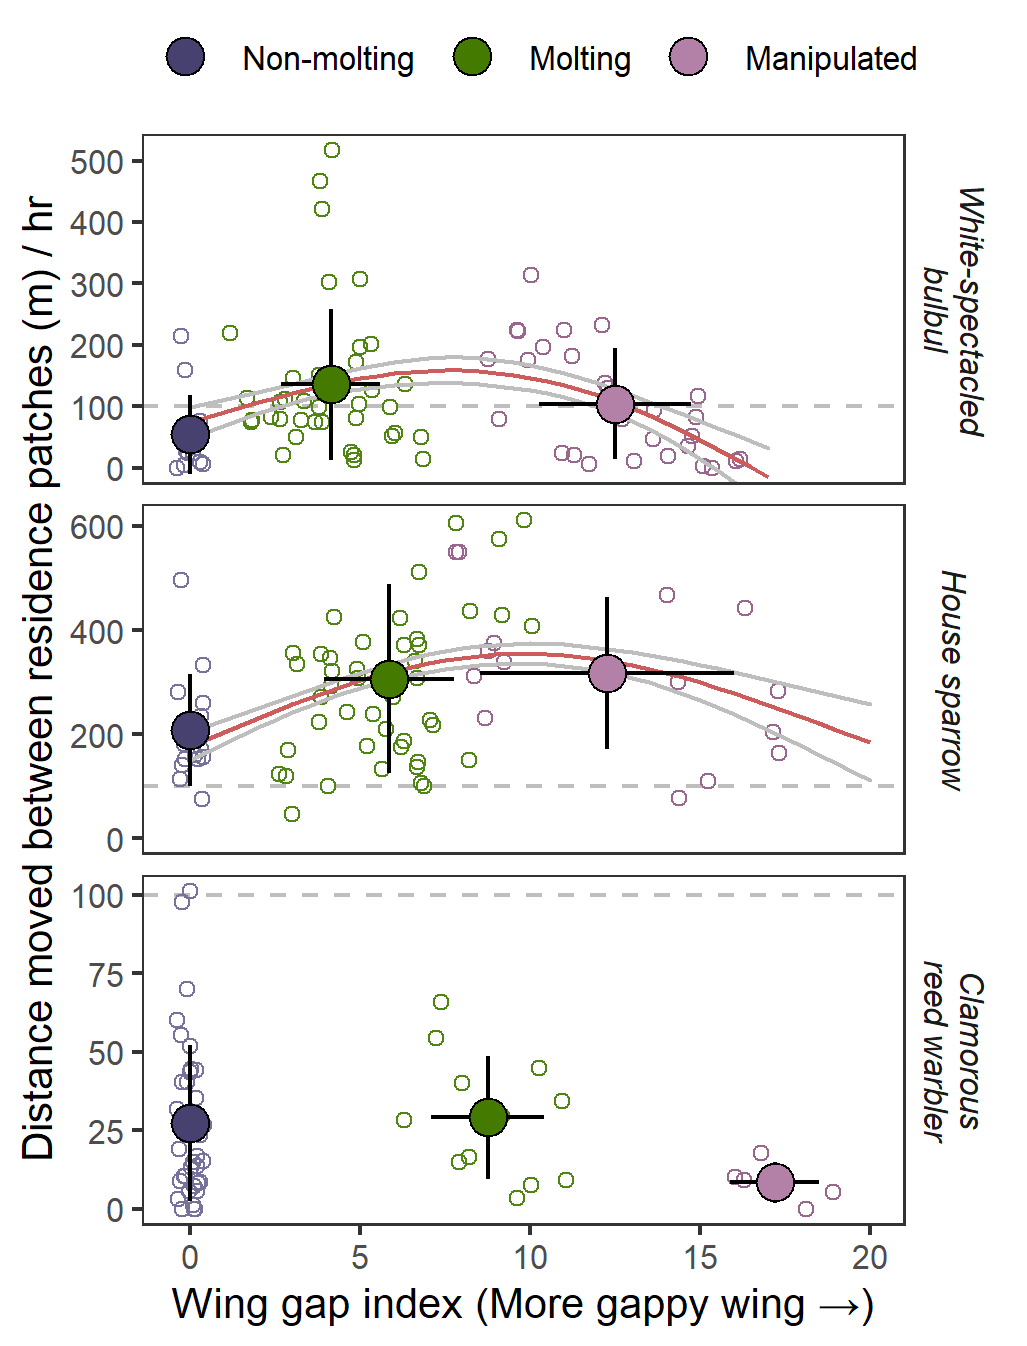
\includegraphics[0.9\textwidth]{figures/holeybirds/fig_01.png}
\caption{
    \textbf{Naturally molting bulbuls and sparrows, but not reed-warblers, move farther between residence patches during natural molt than following experimental feather manipulation.}
    White-spectacled bulbuls (\textit{Pycnonotus xanthopygos}) and house sparrows (\textit{Passer domesticus}) moved 251\% and 150\% as far between areas of prolonged use (`residence patches') when molting, compared to non-molting individuals (see text for statistics).
    %generalised additive model estimates: bulbuls, $F$ = 4.734, p = 0.01; sparrows, $F$ = 11.58, p < 0.001).
    However, when bulbuls' and sparrows' wings were heavily compromised by experimental manipulation (wing gap index $\geq$ 12), both species made shorter movements between residence patches.
    In contrast, clamorous reed-warblers (\textit{Acrocephalus stentoreus}) did not show a significant difference in large-scale movements with increasing wing gap index, possibly because they are already restricted to small patches of reedbeds.
}\label{fig1}
\end{figure}

Of the four species we studied, bulbuls and sparrows are relatively wide-ranging birds, reed-warblers are strongly range restricted to patchy reedbeds, and swallows are very wide-ranging, largely aerial foragers.
Bulbuls and sparrows molt more slowly than reed-warblers, but more rapidly than swallows.
Thus reed-warblers have the largest molt-related wing gaps, swallows the smallest, while bulbuls and sparrows are intermediate between them {(wing gap index, mean $\pm$ SD: swallows = 4.3 $\pm$ 0.95, bulbuls = 4.95 $\pm$ 1.37, sparrows = 5.9 $\pm$ 2.1, reed warblers = 9.5 $\pm$ 1.38)}.
All non-molting birds had a wing gap index score of zero.

\subsection*{Molt-related wing gap size and large-scale movements}

For bulbuls, sparrows, and reed-warblers, we quantified large-scale movements as both the displacements between areas of prolonged residence, called `residence patches' \cite{gupte2022d}, as well as the frequency of these displacements.
Since swallows constantly fly while foraging, we chose to quantify their large-scale movement by simply calculating the total distance moved, adjusting for the daily duration of daytime tracking.
We related total large-scale movements (controlling for daily, daytime tracking duration) with wing gap size using generalised additive models (GAM).
We fit one GAM for bulbuls, sparrows, and reed-warblers (species included as both fixed and random effect), and a separate GAM for swallows (see \textit{Methods}; see \textit{SI Appendix} for model specification).

\begin{figure}[!t]
    \centering
    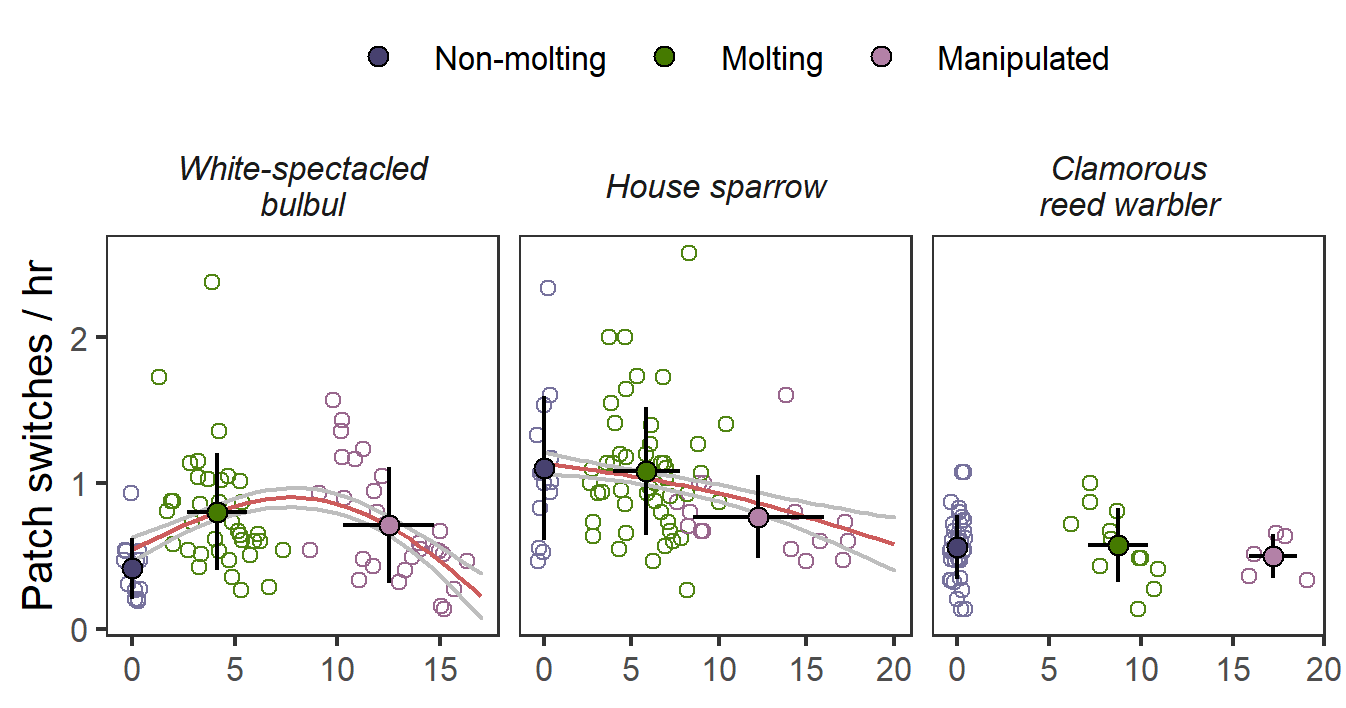
\includegraphics[0.9\textwidth]{figures/holeybirds/fig_02.png}
    % width=8.7cm,height=8.7cm
    \caption{
        \textbf{Patch-switching behaviour is affected by wing gap size in bulbuls and sparrows, but not in reed-warblers.}
        Bulbuls switched between areas of prolonged use (`residence patches') more frequently when molting naturally than when not molting; however, bulbuls whose feathers had been artificially cut (`manipulated') switched less frequently between patches.
        %(generalised additive model [GAM] estimates: $F$ = 7.45, p $<$ 0.001).
        Molting sparrows switched residence patches less frequently with increasing wing gap index; naturally molting birds switched less than non-molting ones, and manipulated birds least of all. %(GAM estimates: $F$ = 3.52, p = 0.024).
        Reed-warblers did not show a significant difference in patch switching with increasing wing gap index, possibly because they are already restricted to small patches of reedbeds.
    }\label{fig2}
\end{figure}

\paragraph*{Distance between residence patches}

We found that bulbuls and sparrows, but not reed-warblers, adjusted their daytime large-scale movements between residence patches to their wing gap size (Fig.~\ref{fig1}; GAM t-value = 2.13, p = 0.034; \textit{SI Appendix} Table S1).
Compared with non-molting individuals (wing gap = 0), naturally molting bulbuls with moderately large molt-related gaps (3 $<$ wing gap $\leq$ 10) actually moved 2.5 times as far per hour between residence patches (GAM estimate $F$ = 4.734, p = 0.01; distance between patches: non-molting = 54.11 m, molting = 135.89 m).
Similarly, naturally molting sparrows moved {1.5 times} as far per hour between residence patches (GAM estimate $F$ = 11.58, p = 0.00002; distance between patches: non-molting = 208 m, molting = 307 m).
This is consistent with the idea that wing molt is an energetically demanding period that requires actively seeking out high-quality food sources \citep{madsen1987a,fox1998}.

Reed-warblers and swallows, which represent very rapid and very slow molt rates, respectively, showed no statistically significant change in large-scale movement with increasing size of the molt-related wing gap (Fig.~\ref{fig1}: reed-warblers).
Rapidly-molting reed-warblers moved similar distances between residence patches when molting or non-molting (GAM estimate $F$ = 0.055, p = 0.815; Fig.~\ref{fig1}).
This is presumably because reed-warblers 
% are already very strongly constrained to a few clustered reedbed habitats, and thus 
do not move between distant patches even when not molting (mean distance between residence patches: non-molting = 27.20 m, molting = 29.09 m, manipulated = 8.49 m) \citep{kiat2016}.
Slow-molting swallows also moved similar (large) distances per hour when they were either non-molting, molting, or artificially manipulated (GAM estimate $F$ = 0.129, p = 0.723).
Swallows' slow molt rate likely represents an adaptation to their aerial foraging habit, allowing them to maintain flight performance across molt stages (non-molting = 3.48 $\pm$ 1.36 km, molting = 3.36 $\pm$ 1.17 km, manipulated = 3.64 $\pm$ 1.96 km).

\paragraph*{Effect of artificial manipulation}

Our experimental manipulation involved removal of one to three primaries, in addition to the primaries missing as part of natural molt (see \emph{Methods}).
Wing gap index scores after artificial manipulation showed differences among species corresponding to their natural molt rate, manipulated reed warblers had larger wing gaps than manipulated swallows, bulbuls, or sparrows {(swallows = 10.11 $\pm$ 2.5, bulbuls = 13.5 $\pm$ 2.35, sparrows = 12.56 $\pm$ 3.5, reed-warblers = 17.8 $\pm$ 1.1).}
Bulbuls and sparrows whose flight feathers had been removed by manipulation (12 $<$ wing gap $<$ 20) moved shorter distances than naturally molting birds {(bulbuls: 68\% less, 43 m; sparrows: 16.7\% less, 256 m)}.
% Bulbuls especially barely moved at all between residence patches when their wings were heavily compromised by artificial manipulation (wing gap $>$ 15; mean distance between residence patches / hr = 39.3 $\pm$ 42.2 m; Fig.~\ref{fig1}).
These observations are in line with the direct effects of severely reduced flight capacity and allocating energy reserves to feather regrowth rather than movement, and an indirect effect of risk-avoidance during a vulnerable period.

\paragraph*{Frequency of patch switching}

We found that in addition to affecting the distance moved between residence patches, the wing gap resulting from natural molt or manipulation also affected the frequency of patch switching in bulbuls and sparrows, but not in reed-warblers (Fig.~\ref{fig2}).
Naturally molting bulbuls moved more often between residence patches than non-molting and artifically manipulated birds (GAM estimate $F$ = 7.45, p $<$ 0.001; see also \textit{SI Appendix} Table S2).
However, naturally molting sparrows switched between residence patches as often as non-molting birds, but artificially manipulated sparrows switched patches less frequently than molting birds (GAM estimate $F$ = 3.515, p = 0.024; Fig.~\ref{fig2}).
Reed-warblers did not show a change in patch-switching frequency in relation to wing gap size (GAM estimate $F$ = 1.04, p = 0.31).

\begin{figure}[!t]
    \centering
    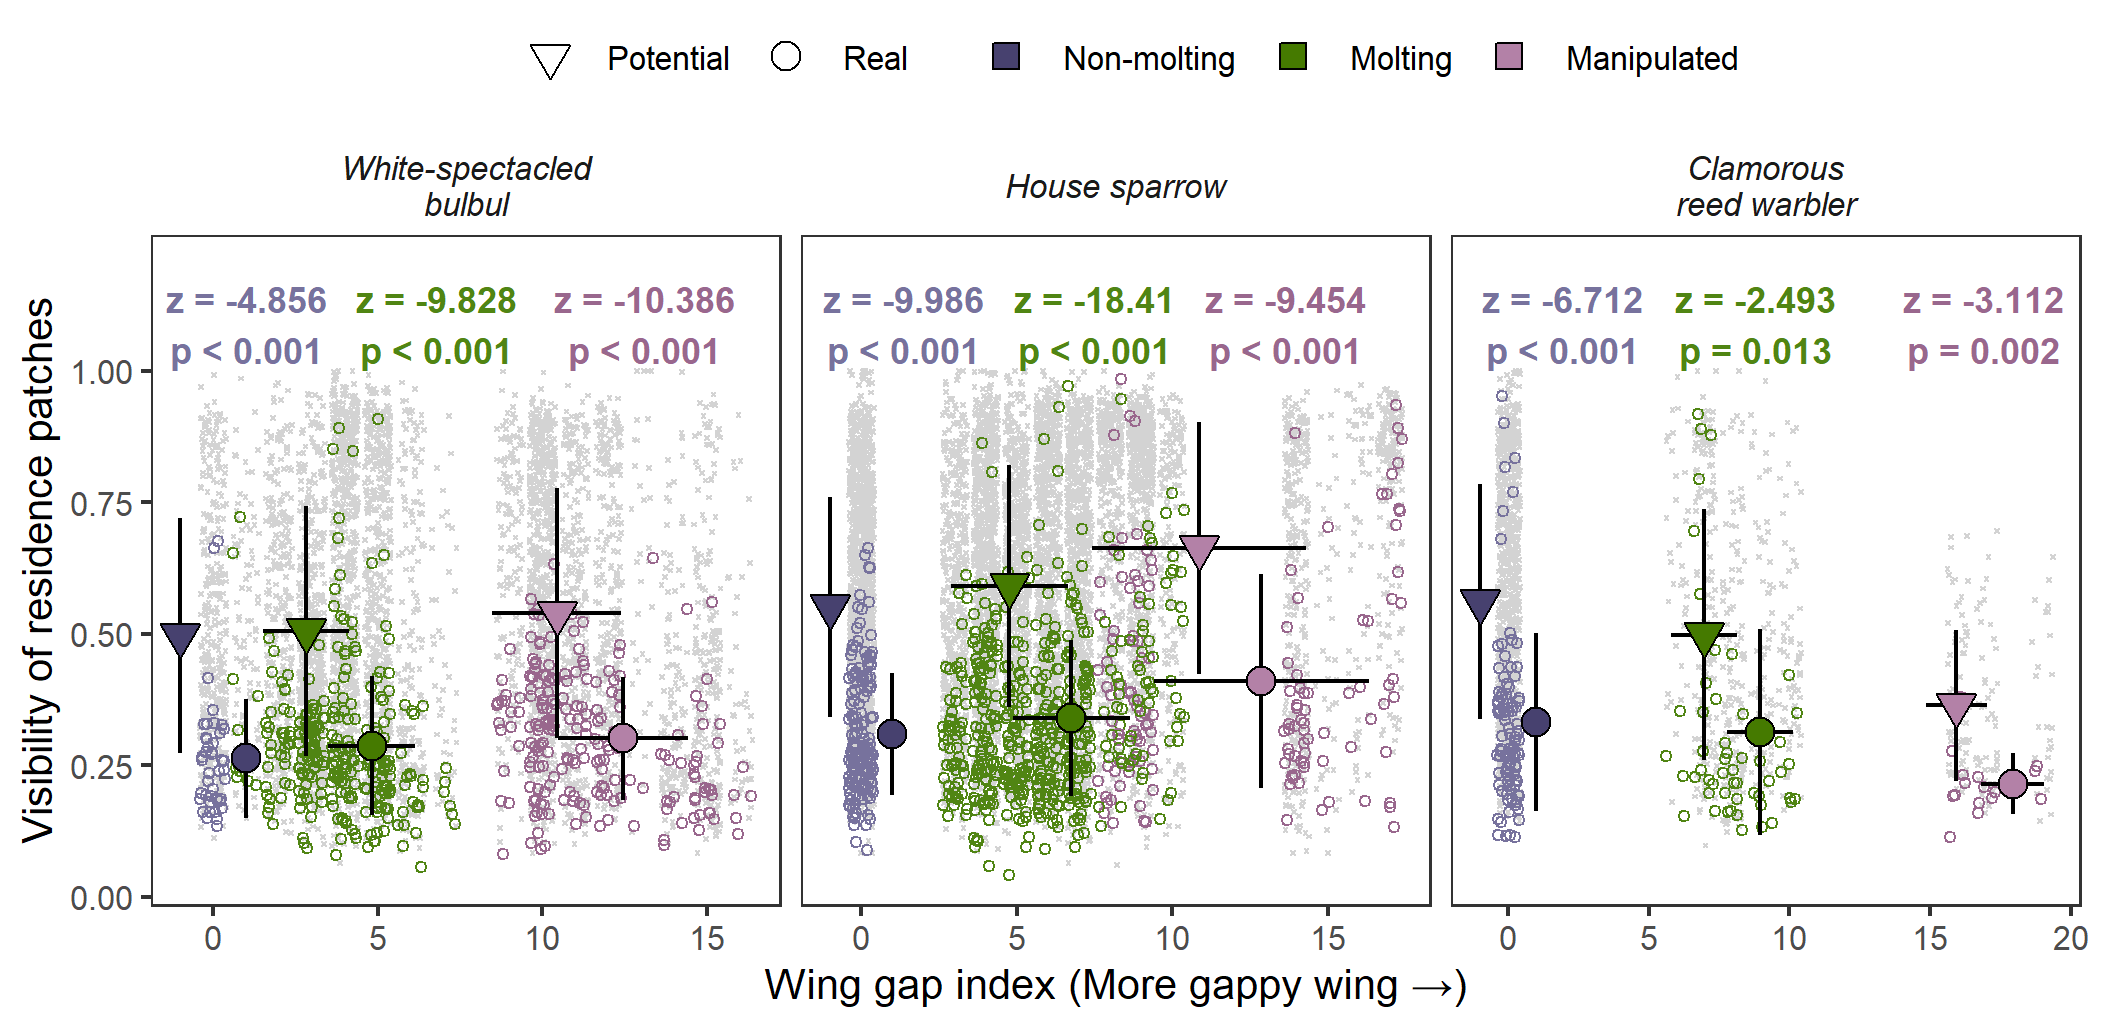
\includegraphics[0.9\textwidth]{figures/holeybirds/fig_03.png}
    % width=8.7cm,height=8.7cm
    \caption{
        \textbf{Naturally molting bulbuls and reed-warblers, but not sparrows, use residence patches for shorter durations than non-molting and artificially manipulated birds.}
        Bulbuls and reed-warblers use contiguous areas for shorter durations when molting, than either when not molting or when some of their flight feathers have been removed by artificial manipulation. 
        %(GAM estimates: bulbuls, $F$ = 18.87, p $<$ 0.001; warblers, $F$ = 12.85, p $<$ 0.001).
        However, sparrows did not show an effect of wing condition on their use of residence patches. %(GAM estimate $F$ = 0.02, p = 0.88).
        The visibility of a patch to low-flying predators reduced the duration for which it was used, %(GAM parametric estimate = -0.70, p = 0.004), 
        but patch vegetation productivity (NDVI) had no effect. 
        %(GAM parametric estimate = 0.05, p = 0.86).
    }\label{fig3}
\end{figure}

\subsection*{Molt-related wing gap size and patch occupancy}

We examined whether the time that bird spent in residence patches was affected by their wing gap size, with the expectation --- following the results for movements between patches --- that molting birds would spend less time in patches than non-molting and manipulated birds (see \textit{SI Appendix} for model specification).
This was indeed the case for both bulbuls and reed-warblers, for which the mean patch duration for molting birds was only about half of that for non-molting and manipulated birds (Fig.~\ref{fig3}; GAM estimates: bulbuls, $F$ = 18.86, p $<$ 0.001; reed warblers, $F$ = 12.854, p $<$ 0.001).
However, we found that sparrows had similar patch durations across different wing gap sizes (GAM estimate $F$ = 0.023, p = 0.878; \textit{SI Appendix} Table S3).

We expected two environmental attributes --- vegetation productivity (NDVI), and visibility to predators --- to also affect patch durations.
To quantify patch visibility, we calculated the visibility index across our study area \cite{olsoy2015,aben2018,aben2021}.
The visibility index represents whether a location can be observed from surrounding areas, for example by a commonly occurring predator, the Eurasian Sparrowhawk (\textit{Accipiter nisus}; see \textit{Methods}).
Areas with taller vegetation such as orchards, and built-up areas such as settlements have lower visibility indices and are more sheltered (see \textit{SI Appendix}), as predators' lines of sight are obstructed by intervening objects \cite{olsoy2015}.
We found that NDVI did not appear to influence patch duration (GAM parametric estimate = 0.056, p = 0.86).
However, patch durations increased with reduced patch visibility (GAM parametric estimate = -0.70, p = 0.004).

\subsection*{Birds occupy sheltered areas across molt rates}

Finding that patch visibility influenced patch durations, we examined whether birds' molt-related wing gaps directly influenced their use of sheltered areas (except swallows, which are aerial foragers).
First, fitting a GAM with species-specific smooths for bulbuls, sparrows, and reed-warblers (see \textit{Methods}), we found that only reed-warblers had slightly more sheltered patches with larger wing gaps (GAM estimate $F$ = 9.30, p = 0.002; Fig.~\ref{fig4}; visibility: non-molting = 0.33 $\pm$ 0.17, molting = 0.31 $\pm$ 0.19, manipulated = 0.21 $\pm$ 0.06), potentially because their rapid molt rate severely reduces flight capacity and makes increased shelter necessary.
% only a moderate overall relationship between the visibility index of residence patches and the size of the molt-related wing gap (GAM t-value = 100.5, p $<$ 0.001; $R^2$ = 0.312).
This suggests that bulbuls and sparrows, with intermediate molt rates, occupy sheltered areas of similar (low) visibility regardless of the size of their wing gap (visibility: bulbuls =  0.39 $\pm$ 0.18; sparrows = 0.47 $\pm$ 0.19; see \textit{SI Appendix} Table S4).

We went one step further, and used a step-selection approach to sample patches to which individuals could have moved, and estimated birds' relative preference for visibility and NDVI when making movement decisions (see \textit{Methods}) \citep{avgar2016,aben2021}.
Fitting separate step-selection functions for each species and each broad molt group (non-molting, molting, and manipulated), we found that across molt group, all three species preferred low-visibility sheltered sites over higher visibility ones (Fig.~\ref{fig4}; \textit{SI Appendix} Table S5).
Furthermore, NDVI did not signficantly affect birds' movement decisions at the patch scale (see \textit{SI Appendix} Table {S1}).
This is consistent with the idea that birds of our study species mostly avoid open agricultural fields, where they might be exposed to potential predators, even though fields are highly productive.

\begin{figure}%
\centering
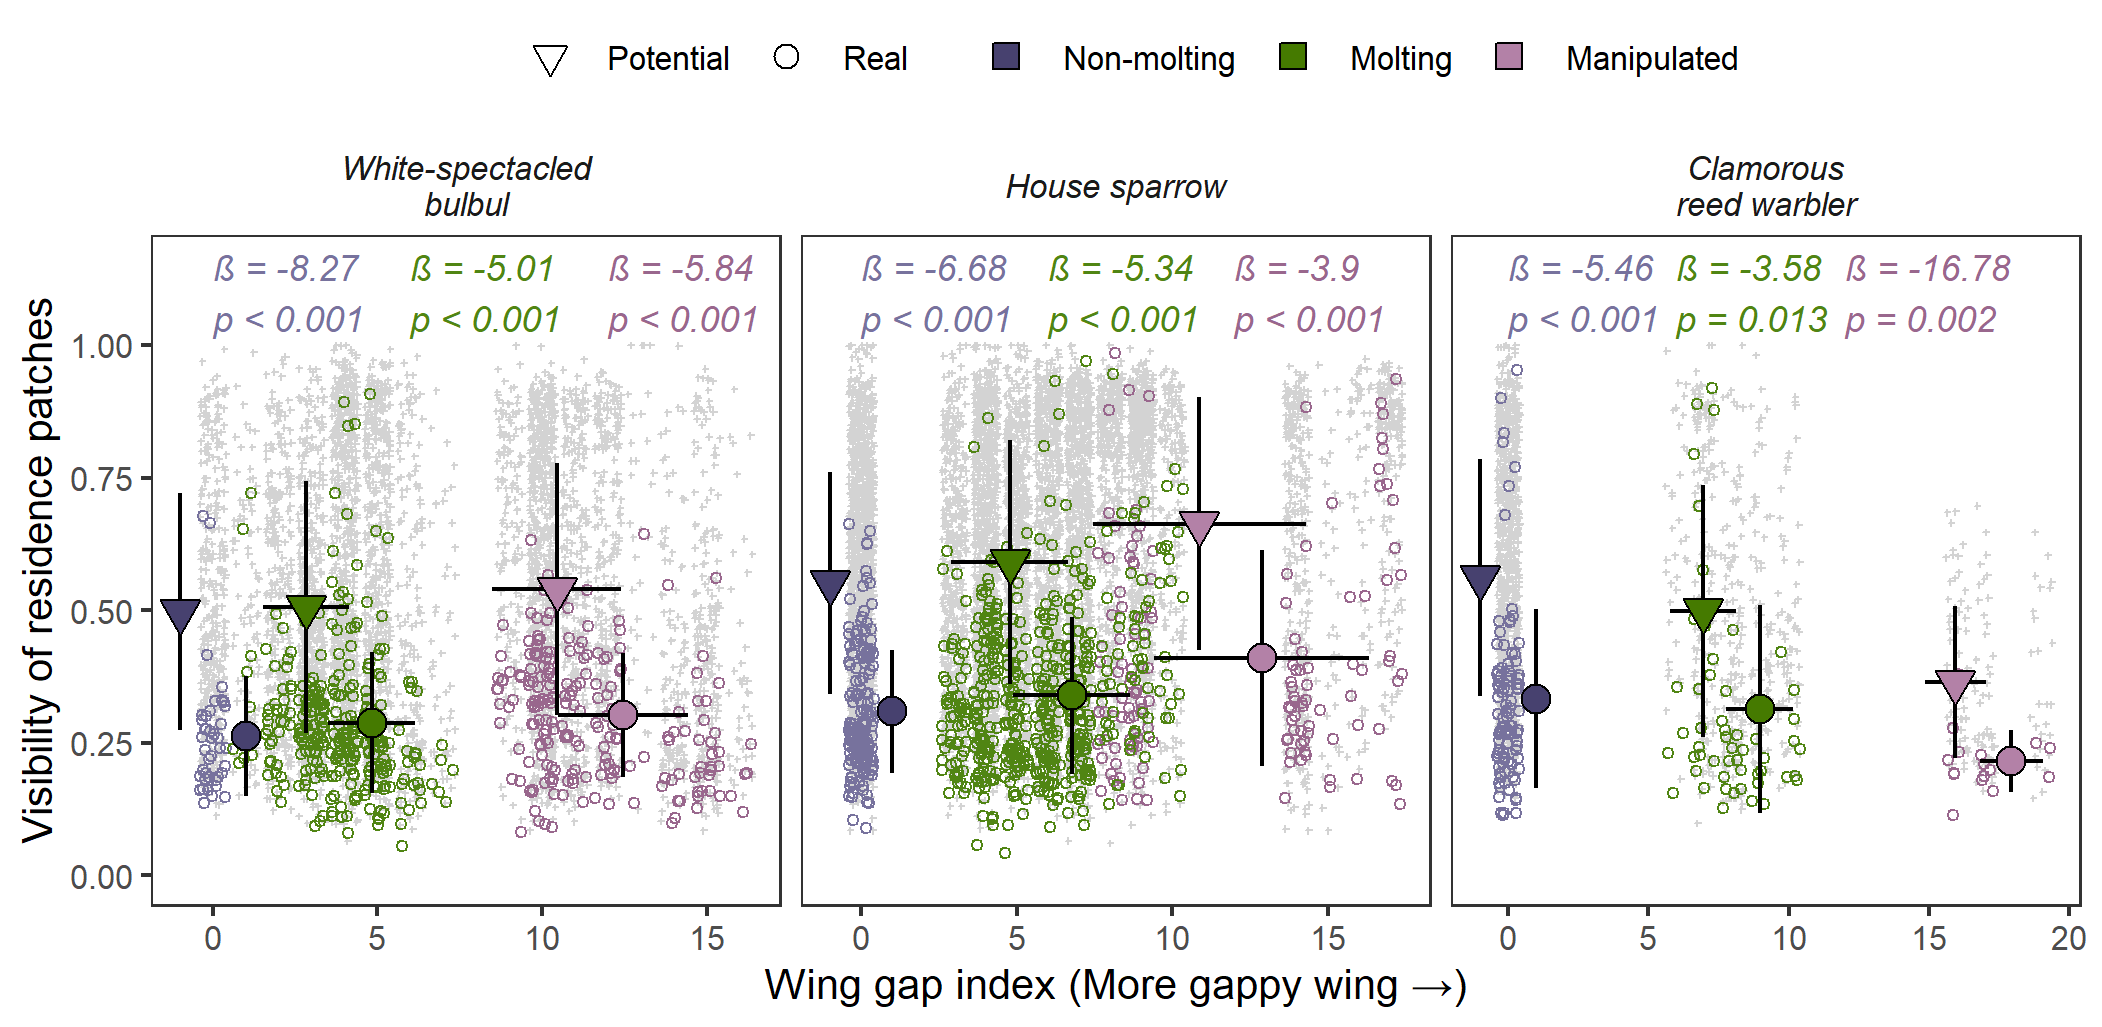
\includegraphics[0.9\textwidth]{figures/holeybirds/fig_04.png}
% width=8.7cm,height=8.7cm
\caption{
    \textbf{Bulbuls, sparrows, and reed-warblers prefer sheltered habitats across wing condition.}
    Across the three species, a GAM indicated that molt-related wing gap index was a poor predictor of the visibility of areas actually occupied by individuals (`real' residence patches; small colored circles). 
    A step-selection analysis at patch level, comparing real residence patches to sampled potential residence patches (grey crosses), showed strong selection for patches with low visibility index scores for all wing conditions, indicated by negative estimated selection coefficients ($\beta$ = natural logarithm of relative selection strength). 
    All $\beta$ values were statistically significant (see \textit{SI Appendix}).
    Filled circles and triangles, and error bars around them, show the mean visibility index of real and potential patches for each molt treatment (indicated by color).
}\label{fig4}
\end{figure}

\section*{Discussion}

Our study is among the first to quantify how the compromised wing surface associated with molt directly affects movement and habitat selection in wild birds.
Our high-throughput tracking system enabled tracking small birds at temporal (several times per minute) and spatial resolutions (a few metres) far surpassing current technologies for tracking such small birds ($<$ 50g) --- mainly through radio triangulation and geolocators, that have low temporal (a few fixes per hour or day, respectively) and spatial resolution (error margins up to 200 km) \citep{bridge2013}.
Focusing on resident birds outside their breeding season, rather than migratory or breeding ones, enables at least some control on confounding factors associated with seasonal physiological changes, and the confounding effect of migration- or breeding-related energy and time requirements \cite{alerstam1990,wikelski2003,horvitz2014}.
Our study also extends the geographic range of the field to an understudied region, and to two less-studied species.

Both rapidly molting clamorous reed-warblers, and slow-molting barn swallows, did not adjust their large-scale movements to their wing condition.
Reed-warblers move very short distances ($<$ 25m) in low-visibility areas, and can afford rapid, resource-intensive feather growth \citep{lindstrom1993,newton2009,kiat2017}, as this does not compromise their ability to move scansorially through their dense reedbed habitat, which also offers shelter from visual predators.
At the other extreme, barn swallows that forage exclusively while flying have evolved a very slow molt rate \cite{kiat2016}, which likely forestalls significant direct aerodynamic effects of feather loss on flight capacity.
Our work shows how birds' evolved molt strategies --- which are themselves influenced by movement strategies \cite{kiat2016} --- are interlinked with the direct, short-term effects of molt on movement.

We also found that birds with intermediate molt rates --- white-spectacled bulbuls and house sparrows --- adapt their movement strategies to their wing morphology.
Surprisingly, these species moved more when naturally molting than non-molting.
Birds can compensate for lower wing power output by growing their pectoral muscles, and this may allow them to maintain flight capacity during the molt, enabling increased movement to find resources for feather growth \cite{chai1997,swaddle1997}.
Unsurprisingly, increased movements between putative foraging patches, and an increased frequency of such movements, together translate into a shorter occupancy duration in each patch.
While this movement strategy conforms with optimal foraging theory --- rapid abandonment of patches to maximize prey intake \cite{charnov1976} --- it does not appear that vegetation productivity influences patch use.

When increased movement for high quality resources \cite{charnov1976} cannot compensate for the costs of inefficient flight and feather growth, moving less overall to conserve energy may be the optimal strategy until new flight feathers develop.
This latter strategy should be expected when the wing gap size is increased beyond the extent of natural molt, as found in our study.
The shorter between-patch movements of artificially manipulated sparrows and bulbuls with especially large wing gaps (wing gap index $>$ 12), compared with natural molt, thus fit within this hypothesis.
Importantly, our relatively non-invasive method only increases the wing's feather gap size while avoiding wing injury, suggesting that the reduction in flight is actually due to considerations of flight efficiency, rather than trauma.

We have for the first time applied the idea of the cumulative viewshed to directly assess the availability of shelter from visual predators, along birds' real and potential movement paths \cite{olsoy2015}.
Birds, like other animals, are capable of taking the spatial perspective of other individuals \cite{emery2000,krams2001,watve2002,davidson2016}, i.e., whether a location would be visible to another observer, such as a predator \citep{watve2002,olsoy2015}.
Previous work has focused on demonstrating spatial perspective taking --- and resulting habitat selection --- at small spatial scales of a few metres, and typically with a direct predator cue \cite{krams2001,watve2002}.
Our work is the first to combine the spatial perspective-taking concept with the emerging framework of animal viewshed ecology at landscape scales \cite{aben2018,aben2021}.
Our findings suggest that birds can estimate the visibility (and hence riskiness) of an area from multiple perspectives, and that they can do so at relatively large, landscape scales (many dozens of metres).
Our results also show how the modelling of animal movement decisions should incorporate individuals' estimates of what \textit{other animals} can see \cite{hampton1994,emery2000}.
Visibility analysis provides a simple, mechanistic way to incorporate animals' potential assessments of landscape risk into habitat selection models.
This could help move away from purely correlative studies of animal habitat selection, which usually rely on predictors with very broad applicability \cite{pettorelli2011}.

All three species studied strongly preferred sheltered, low-visibility habitats over more open sites, even when the available sites had similar vegetation productivity.
Predators are unlikely to always be in the vicinity of a specific location, or indeed to always be visible.
This instead points to an avoidance of open agricultural areas where predation risk is highest, showing the immediate, small-scale effects of a `fearscape' \cite{olsoy2015} on animal movement.
This pre-emptive caution may explain why wing condition, which should be expected to determine vulnerability to predation, did not lead to more sheltered residence patches in two of three relevant species.
Furthermore, our findings suggest that avoidance of high-visibility areas may be an overlooked, yet potentially broadly applicable mechanism by which agricultural `green deserts' exclude avian biodiversity.
An unwillingness to break cover from sheltered areas, and move through high-visibility habitat, may explain how individual movement decisions can scale up to restrict animal space use, from short home-range moves to longer dispersal events \cite{schlagel2020}.
Overall, our work provides a template for combining simple experimental methods with technological advances in tracking technology, and with a mechanistic approach to landscape ecology, in animal movement research.

\section*{Acknowledgments}

This study was supported by the Minerva Center for Movement Ecology, the Minerva Foundation, and ISF grant ISF-965/15 to R.N and S.T, and ISF grant 1919/19 to S.T. We also thank the Survey of Israel for their generous help. 
P.R.G was supported by an Adaptive Life Programme grant made possible by the Groningen Institute for Evolutionary Life Sciences (GELIFES), and by the European Research Council (ERC Advanced Grant No. 789240 awarded to F. J. Weissing).
R.N also acknowledges support from the Adelina and Massimo Della Pergola Chair of Life Sciences.

\newrefcontext[sorting=nyt]
\section*{Literature Cited}
\printbibliography[title={Literature~Cited},heading=none]
\end{refsection}

\cleardoublepage %************************************************
\chapter{Land-cover and Climate Shape Bird Distributions in a Tropical Biodiversity Hotspot}\label{ch:hillybirds}
\chaptermark{Citizen Science \& Bird Distributions}
%************************************************
% Using citizen science to parse climatic and land cover influences on

{\noindent \sffamily Vijay Ramesh\textsuperscript{1}, \textbf{Pratik R. Gupte}, Morgan Tingley\textsuperscript{2}, V.V. Robin\textsuperscript{3}, and Ruth S. de Fries\textsuperscript{1}}

\marginpar{
    \sffamily
    \textsuperscript{1} Columbia University, USA.
    
    \medskip
    
    \textsuperscript{2} University of California --- Los Angeles, USA.
    
    \medskip

    \textsuperscript{3} Indian Institute for Science Education and Research --- Tirupati, India.
}

\section*{Abstract}

\marginpar{ 
    \bigskip

    {\large{$\Delta$}} \normalfont Under review at \textit{Ecography} as Ramesh et al. Using citizen science to parse climatic and land cover influences on bird occupancy within a tropical biodiversity hotspot.
}

\small{
    Disentangling associations between species occupancy and its environmental drivers --- climate and land cover --- along tropical mountains is imperative to predict species distributional changes in the future.
    Previous studies have primarily focused on identifying such associations in temperate mountain systems.
    Using 1.29 million robustly processed citizen science observations contributed to eBird between 2013 and 2021, we examined the role of climatic and landscape variables and its association with bird species occurrence within a tropical biodiversity hotspot, the southern Western Ghats in India.
    Using an occupancy modeling framework, we found that temperature seasonality, precipitation seasonality, and the proportion of evergreen forests were significantly associated with species-specific probabilities of occupancy for 78\% (n = 43 birds), 38\% (n = 21 birds), and 27\% (n = 15 birds) of bird species examined, respectively.
    Our study shows that several forest birds (n = 18 species) were negatively associated with temperature seasonality, highlighting narrow thermal niches for such species.
    The probability of occupancy of six forest species and eight generalist species was positively associated with precipitation seasonality, indicating potential associations between rainfall and resource availability, and thereby, species occurrence.
    A smaller number of largely generalist species (n = 9 birds) were positively associated with human-modified land cover types --- including the proportion of agriculture/settlements and plantations.
    Our study shows that rigorously filtered citizen science observations can be used to identify associations between environmental drivers and species occupancy on tropical mountains.
    Though current distributions of tropical montane birds of the Western Ghats are strongly associated with climatic factors (mainly, temperature seasonality), naturally occurring land cover types (forests) are critical to sustaining montane avifauna across human-modified landscapes in the long run.
}

\clearpage



\newrefcontext[sorting=ynt]

\lettrine{T}{ropical} montane ecosystems are hotspots of biological diversity and are home to over 70\% of the world's avian diversity in less than 10\% of global terrestrial area \citep{myers2000,davies2007,quintero2018}.
However, tropical mountains are under tremendous anthropogenic pressures of habitat modification and climate change, which can both have negative consequences for bird species \citep{nogues-bravo2007,newbold2015}.
In addition to directly affecting bird populations, climate change and changes in land cover can also affect species distributions in montane areas worldwide \citep{nogues-bravo2007,rahbek2019}.
For example, mountain birds in California tracked changes in temperature and precipitation over a century of climate change, illustrating the long-term role of climate in driving range shifts \citep{tingley2009}.
The movement of temperature bands upslope can eliminate the conditions to which high-altitude species are adapted, leading to local extinction \citep{freeman2018,urban2018}.
A combination of changes in climate and land cover best explains the colonization and extinction probabilities of North American birds \cite{yalcin2018}.
However, few studies have disentangled the role of these two drivers on species' current distributions \citep{sirami2017}.
Furthermore, species distributions in tropical mountains especially are poorly studied despite being `escalators to extinction' for montane birds \citep{elsen2017,freeman2018,srinivasan2019,srinivasan2021}.
Understanding the contemporary drivers of species' distributions in tropical mountains can help predict future species ranges as the climate changes \citep{guo2018,srinivasan2021}.

The drivers of bird distributions in tropical montane ecosystems are poorly understood because data on species distributions in these regions are limited \citep{payne2017,peters2019}.
Citizen science efforts offer a solution: initiatives such as \textit{eBird} are growing in popularity and scale and make the observation data readily available to researchers \citep{sullivan2014}.
\textit{eBird} combines many thousands of decentralized, ad hoc, organized, or semi-organized bird observations to form representative samples of species' occurrence over vast scales \citep{sullivan2009,sullivan2014,wood2011a}.
The standardization of the reporting infrastructure (e.g., the \textit{eBird} mobile app or website) allows observations to be reproducibly processed to achieve a high standard of reliability.
For example, one can filter out short observation sessions that might not accurately capture a location's bird community or weight observations by the observer's effort \citep{kelling2015a,johnston2018,johnston2021}.
Including data from citizen scientist observations can significantly improve species distribution models \citep{robinson2020}, and enable a wide range of research, including mapping species elevational movements \citep{tsai2020} and prioritizing conservation efforts \citep{vanstrien2013,fink2014,johnston2015}.
India reports one of the largest numbers of \textit{eBird} checklists from a tropical country, as birdwatchers have contributed to \textit{eBird} in a concerted and growing effort since 2014 \citep{viswanathan2020}.
Coordinated citizen science efforts have led to successfully mapping the distribution and abundance of birds across multiple regions in India \citep[e.g. the Mysore Bird Atlas, and the Kerala Bird Atlas][]{praveenj2021}.
As of March 2021, the \textit{eBird} India dataset has grown to a total of over 14 million observations across 1,342 species of birds.

We set out to examine the role of climate and land cover and its association with bird occupancy in a tropical montane region, the Western Ghats of southern India.
The Western Ghats mountain ecosystem is part of the Western Ghats-Sri Lanka biodiversity hotspot and is home to numerous species of endemic plants and animals \citep{myers2000,das2006}.
We examined observations from \textit{eBird} between 2013 and 2021 for 79 species (later reduced to 55, following model fitting) of birds across the two largest hill ranges in the southern Western Ghats --- the Nilgiri and the Anamalai-Palani hills (see Fig.~\ref{hilly_fig_01}a).
Specifically, we tested associations between climatic variables, land cover, and bird occupancy.
We binned species according to their habitat preference prior to hypothesis testing; a species could either be a forest species (species found in forested/woodland habitats as well as forest edges) or generalist species (widespread species found across a range of habitat types) \citep{ali1983}.

First, we examined the direction of association between species-specific probability of occupancy and climatic predictors.
Temperature seasonality: We tested the hypothesis that the probability of occupancy of forest specialist birds should be negatively associated with temperature seasonality (coefficient of variation) \citep{srinivasan2018}.
Tropical forest species are often associated with a narrow range of temperatures leading to the expectation that the probability of occupancy will decrease with increasing variation in temperatures \citep{janzen1967,stevens1989,frishkoff2016,chan2016,srinivasan2018}.
However, we expected that the occupancy of generalist species may be positively associated with temperature seasonality.
In other words, we expected that generalist species have broader thermal niches and occur in climatically variable regions when compared to their forest counterparts.
Precipitation seasonality: the `hygric' niche hypothesis states that species often occur within an optimal range of rainfall conditions \citep{boyle2020}.
Across our study area, we expected that precipitation seasonality (coefficient of variation) would be positively associated with species occupancy for forest birds and negatively associated with generalist bird species.
Forest species in the Western Ghats are largely seen in wetter habitats relative to generalist species that are more often found in drier habitats \citep{raman2006}.
Finally, we examined the direction of association between species-specific probability of occupancy and land cover.
We expected the occupancy of forest species to be positively associated with naturally occurring land cover types such as evergreen forests and deciduous forests.
We expected that human-modified land cover types, including agriculture, settlements, and plantations would be positively associated with species-specific probability of occupancy of generalist birds.

\subsection*{Methods}

\subsubsection*{The Southern Western Ghats}

The Nilgiri and the Anamalai-Palani hills (hereafter, Anamalai hills) (Fig.~\ref{hilly_fig_01}) are part of the Western Ghats, an ancient region of differentiation of flora and fauna in South Asia \citep{mani1974,myers2000,vijayakumar2016}.
These hill ranges host a diversity of land cover types, possess a wide climatic gradient, and several bird species \citep{ali1983,das2006}.
The elevational range across these hill ranges varies from 40m in the plains to 2,625m in the higher elevations.
(Fig.~\ref{hilly_fig_01}a).
These two hill ranges are home to a multitude of habitats, ranging from high elevation grasslands (>1400 m; Fig.~\ref{hilly_fig_01}b) to mid-elevation evergreen forests (>700m and <1400 m; Fig.~\ref{hilly_fig_01}b).
These hill ranges interact strongly with the annual south-west monsoon resulting in orographic rainfall on the western slopes ($\sim$3000 mm) and a relative rain-shadow on the leeward eastern slopes ($\sim$2000 mm) that in turn influences the distribution of endemic flora and fauna \citep{gadgil1986,pascal1988,robin2015}.

\begin{figure}[h!]
    \centering
    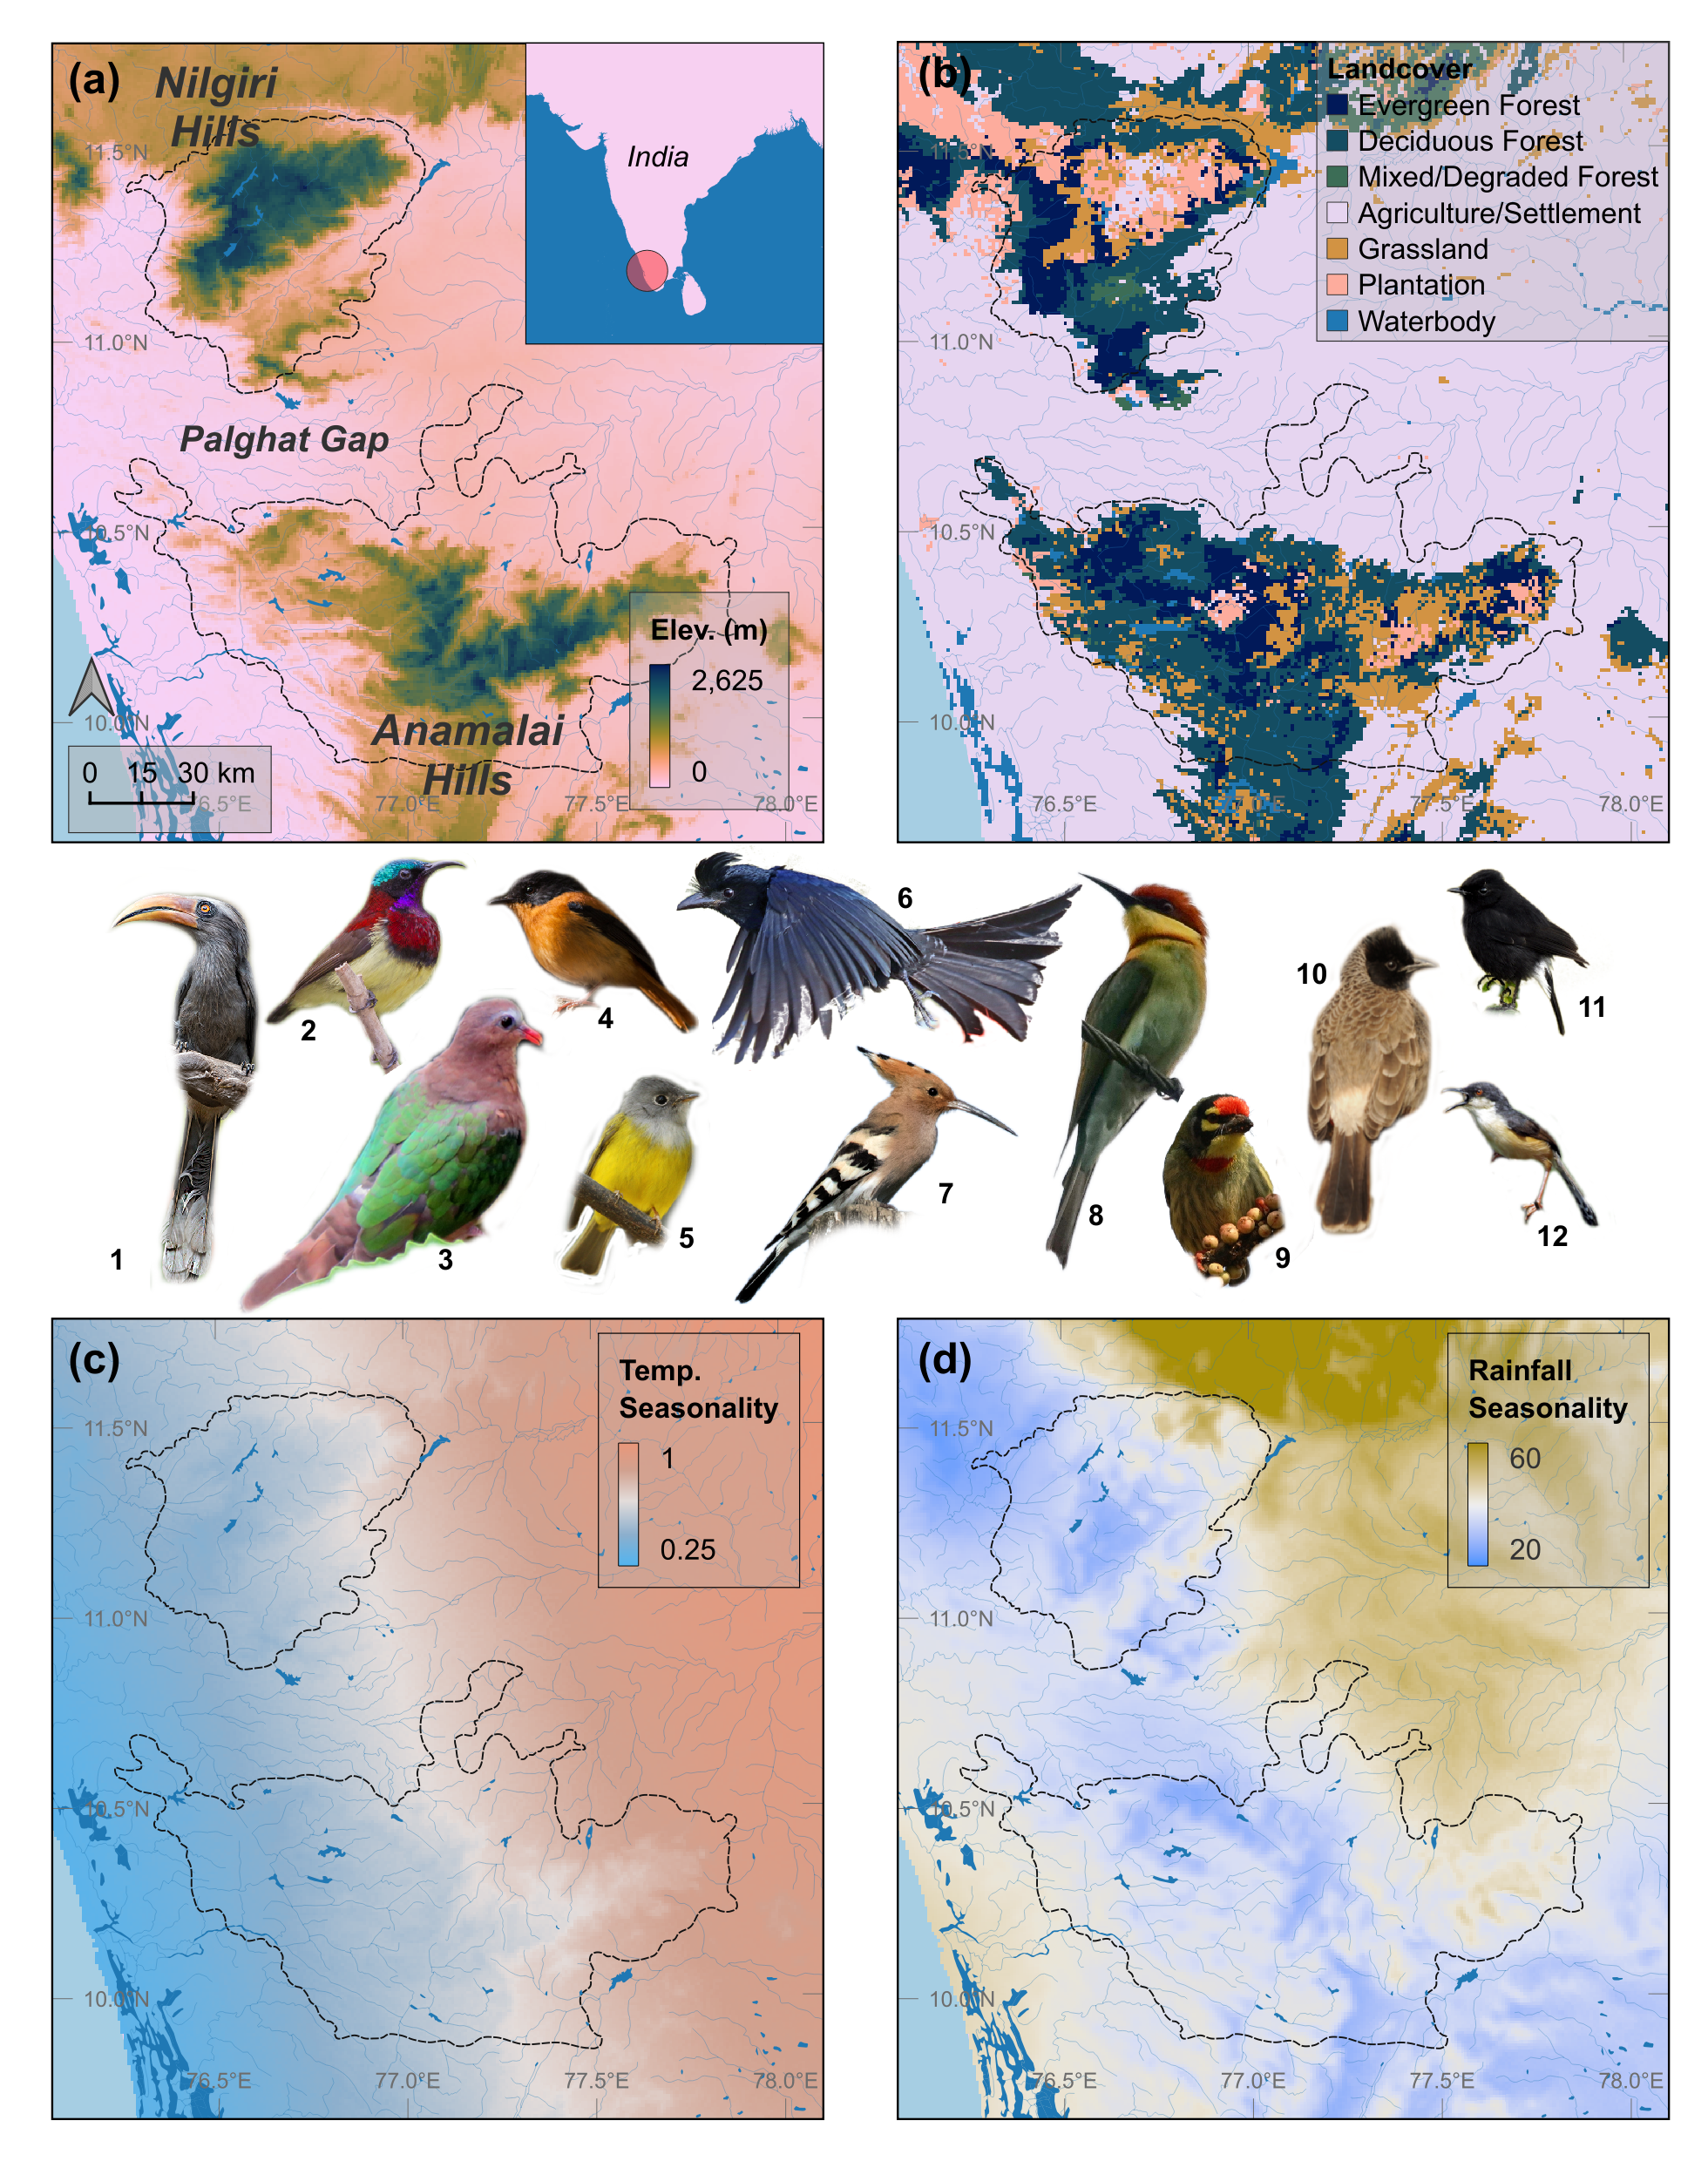
\includegraphics[width=0.9\textwidth]{figures/hillybirds/fig_01.png}
    \caption{
        \textbf{The Nilgiri and Anamalai Hills in southern India provide a convenient geography for studying the interplay of land cover and climate on the distributions of bird species.}
        \textbf{(a)} The Nilgiri and Anamalai Hills of the Southern Western Ghats are topographically complex, with maximum elevations > 2,000 m, and are separated by the very low-lying Palghat Gap, which serves as a natural barrier to the dispersal of many hill birds. 
        \textbf{(b)} Lower elevations are primarily covered by agriculture and settlements, reflecting the intense human pressure on this region, while mid- and higher elevations show a mix of natural and human-modified land cover types (see Fig.~\ref{hilly_fig_02} for details). 
        \textbf{(c)} The coastal edge of the area, and the windward hill slopes show limited temperature seasonality across the December -- May period; this seasonality increases with distance from the coast but is lower at higher elevations inland. 
        \textbf{(d)} Higher elevations also show limited precipitation seasonality than both low-lying coastal and inland regions. 
        Our study area (bounds shown as dashed lines) includes multiple combinations of elevation, land cover type, and temperature and rainfall seasonality, resulting in a naturally occurring crossed-factorial design that allows us to study the effects of climate and land cover on bird occupancy. 
        Representative forest-restricted and habitat-generalist birds from the study area are shown between panels (all images were obtained from Wikimedia commons and credit is assigned for each species in brackets).
        % ; From L to R: (1) Malabar grey hornbill (by Koshy), (2) Crimson-backed sunbird (by Mandar Godbole), (3) Asian emerald dove (by Selvaganesh), (4) Black-and-orange flycatcher (by LKanth), (5) Grey-headed canary flycatcher (by David Raju), (6) Greater-racket tailed drongo (by MD Shahanshah Bappy), (7) Eurasian hoopoe (by Zeynel cebeci), (8) Chestnut-headed bee-eater (by Mik\textit{eBird}s), (9) Coppersmith barbet (by Raju Kasambe), (10) Red-vented bulbul (by TR Shankar Raman), (11) Pied bushchat (by TR Shankar Raman), (12) Ashy prinia (by Rison Thumboor). 
        Elevation is from 30m resolution SRTM data (Farr et al. 2007), land cover, at 1 km resolution, is reclassified from Roy et al. (2015), while climatic variation is represented by CHELSA seasonality layers (temperature: BIOCLIM 4a, rainfall: BIOCLIM 15), at 1km resolution (Karger et al. 2017). All layers were resampled to 1 km resolution for analyses.
    }
    \label{hilly_fig_01}
\end{figure}

\begin{figure}[h!]
    \centering
    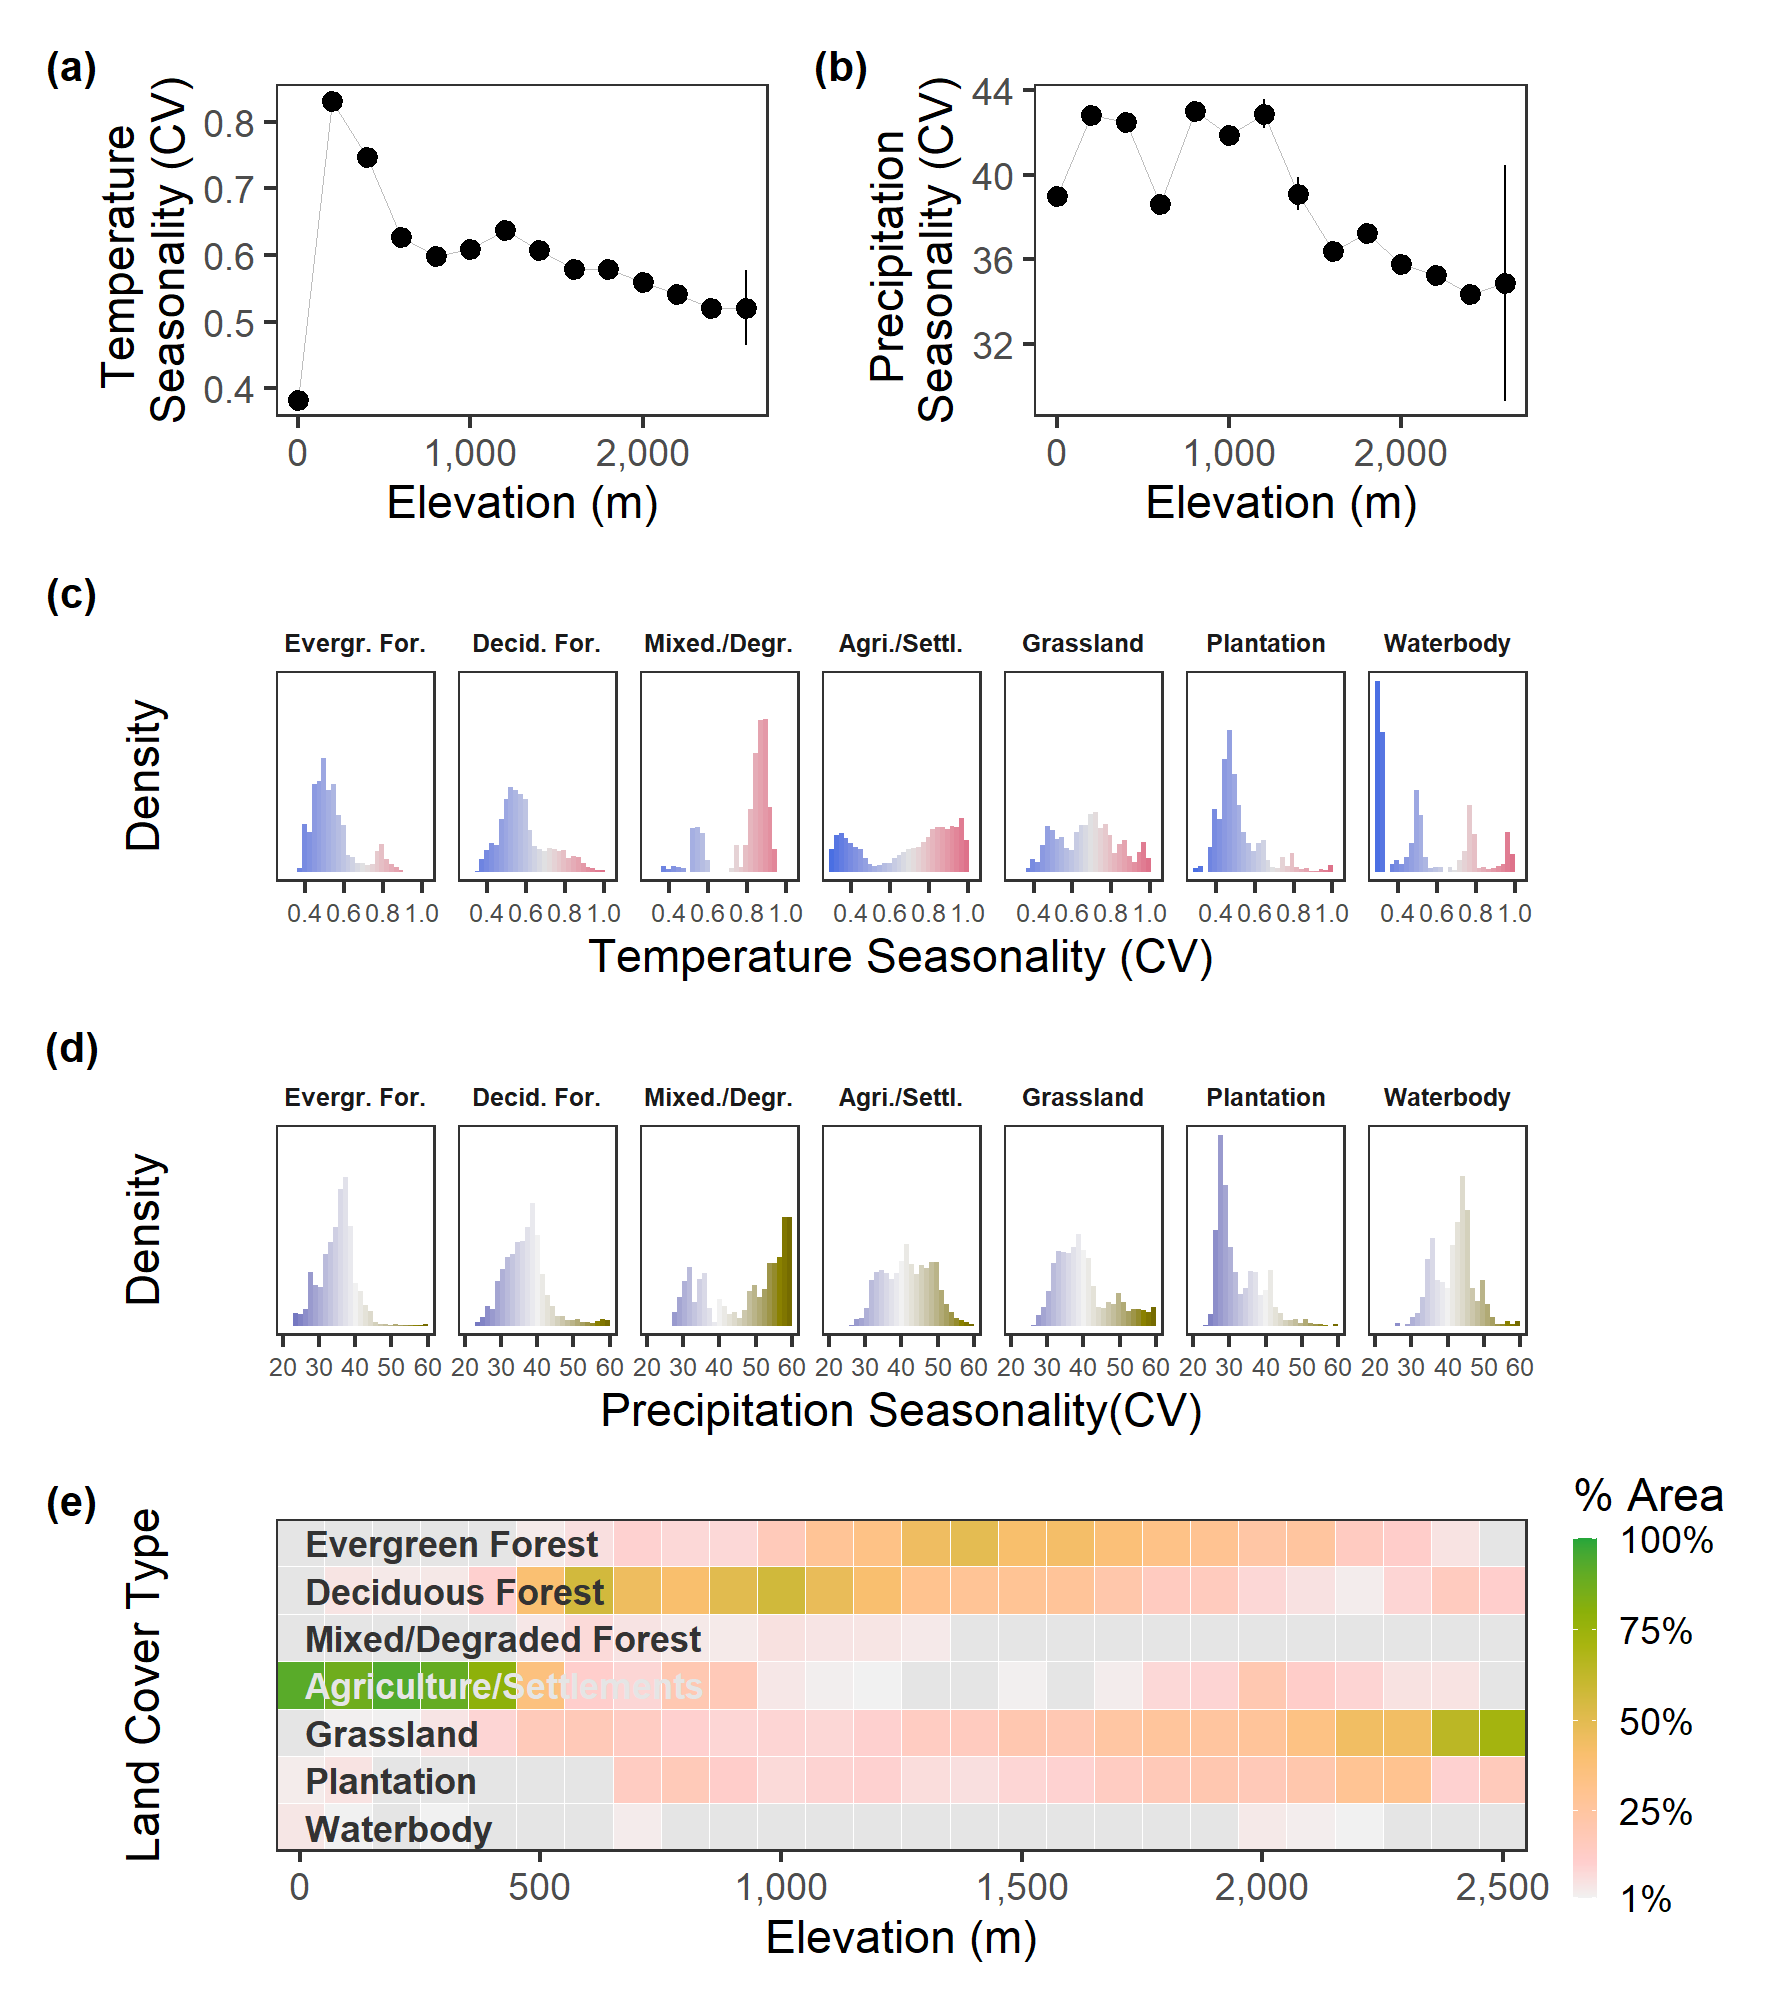
\includegraphics[width=0.9\textwidth]{figures/hillybirds/fig_02.png}
    \caption{
        \textbf{Climate and land cover vary strongly along the elevation gradient in the Nilgiri and Anamalai Hills.}
        Both \textbf{(a)} temperature seasonality and \textbf{(b)} precipitation seasonality, between the months of December and May, declines with increasing elevation across the Nilgiri and Anamalai Hills. 
        Climatic variation is not very strongly associated with land cover type, as both natural habitats such as forests, and human-associated habitat types such as plantations show low seasonality in \textbf{(c)} temperature, and \textbf{(d)} precipitation.
        \textbf{(e)} Most elevations host a range of land cover types: while human-associated habitats such as agriculture are concentrated at lower elevations, and more natural types such as grasslands and forests are associated with higher elevations, each of these types is also found outside their characteristic elevational bands.
        We calculated climate seasonalities (BIOCLIM 4a and 15: temperature and precipitation, respectively) using CHELSA data over 1979 -- 2013, from December to May (Karger et al, 2017), and present mean seasonality values (vertical bars show standard deviation) for every 200m elevational band
        Land cover types were taken from a reclassification of Roy et al
        (2015; see main text) at 100m elevational bands.
        Land cover types covering < 1\% of an elevational band are shaded grey
        All landscape layers were first resampled to 1 km resolution.
    }
    \label{hilly_fig_02}
\end{figure}

\subsubsection*{Filtering \textit{eBird} Data}

Data from \textit{eBird} is available in the form of a `checklist' submitted by an observer or a group of observers.
Each checklist includes a wide range of information that includes species identity, latitude, longitude, date of observation, distance traveled, time spent observing etc.
`Complete' checklists indicate that the observer(s) recorded all the birds detected and identified.
We obtained bird detections from such complete checklists contributed to \textit{eBird} for nine years (2013 to 2021) across the Nilgiri and Anamalai hill ranges.
Only checklists recorded during December to May (non-rainy months) were included in our study because detecting birds during the rainy months is difficult due to poor weather.
Restricting our data to complete checklists also allowed us to interpret the absence of a species on a checklist as a non-detection \citep[called zero-filling][]{johnston2021}.
Even when restricting analysis to only `complete' checklists, the semi-structured, flexible nature of databases like \textit{eBird} results in large variation in effort across checklists as a result of the often opportunistic nature of data collection \citep{kelling2019}.
Complete checklists are marked as `Stationary' or `Traveling' based on the distance traveled by an observer while recording detections.
To reduce variation in observer effort, we first considered only those complete checklists with a duration ≤ 300 mins (5 hrs), and distance ≤ 5 km (for traveling checklists), and with fewer than 10 observers \citep[following][]{johnston2019}.
Since stationary birdwatchers can detect birds up to 100m away, we set all stationary checklists to a distance of 100 m.
In many cases, checklists are submitted by a single observer for a group of birdwatchers; in such cases, the group checklist only occurs once in the dataset.
We used only checklists recorded between 5:00 AM and 7:00 PM to avoid sightings in low-light conditions.

\subsubsection*{Selecting Study Species}

We limited our study to 79 species of terrestrial, diurnal birds that occur in our study region (see list of species in {\color{red}Appendix S1}; see Fig.~\ref{hilly_fig_01} for representative species).
We selected these species using inclusion criteria adapted from the State of India's Birds Report 2020 \citep[SoIB][]{viswanathan2020}.
We intended these criteria to ensure uniform sampling of each species across our study area, and to reduce erroneous associations between environmental drivers and species distributions.
Beginning with 3.37 million observations of 684 species in \textit{eBird} that occurred within the outlines of our study area (Fig.~\ref{hilly_fig_01}a), over the years 2013 -- 2021, we retained only those species that had a minimum of 1,000 detections each between 2013 and 2021 (347 species remaining; 3.33 million observations).
Next, we divided the study area into 25 $\times$ 25 km grid cells (42 unique cells; see supplementary material).
We kept only those species that occurred in at least 5\% of all checklists across at least 27 unique grid cells (50\% of the study area).
We further manually removed raptors (\textit{Accipitriformes} and \textit{Falconidae}), swifts (\textit{Apodiformes}), and swallows (\textit{Hirundinidae}) since these birds are usually observed in flight when species identification can be prone to errors.
This filtering process resulted in a total of 1.29 million observations (presences) across our study area.

\subsubsection*{Spatio-temporal bias in occurrence data}

Sampling bias can be introduced into citizen science observations due to the often opportunistic nature of data collection \citep{sullivan2014}.
For \textit{eBird}, this translates into checklists reported when convenient, rather than at regular or random points in time and space, leading to non-independence in the data if observations are spatio-temporally clustered \citep{johnston2021}.
For example, sites near roads are easier to reach and maybe sampled more frequently.
The spatial clustering of observations can be reduced by sub-sampling at an appropriate spatial resolution \citep{aiello-lammens2015}; however, thinning the data over-zealously can result in very few presence records compared to absence records \citep[i.e., class imbalance][]{steen2019}.
Consequently, when there are many more absence records than presence records, presences and absences should be handled separately when spatially thinning the data.

We first estimated two simple measures of spatial clustering: the distance from each site to the nearest road \citep[road data from OpenStreetMap:][]{openstreetmapcontributors2017} and the nearest-neighbor distance for each site.
Sites were strongly tied to roads (see Fig 3a.; mean distance to road ± SD = 390.77 ± 859.15 m; range = 0.28m -- 7.64 km) and were on average only 297m away from another site (SD = 553 m; range = 0.14m -- 12.85 km).
This is understandable, as roads and trails provide access, and particular well-known areas are visited often.
On average, across species, presences comprised only 8.5\% of all observations.
We followed \textcite{steen2021} in choosing to spatio-temporally thin only the absences, and not the presences, for each species --- a methodology called `thin majority' that can improve model performance \citep{steen2021}.
To do this, we divided the study area into a grid of 500m wide square cells, and from within each cell, we chose the site with the most visits (checklists) over the sampling period.
From each of the remaining sites, we selected a maximum of 10 random absence checklists to reduce temporal clustering, keeping all absence checklists for sites with ≤ 10 checklists.
We retained all presences for each species without any spatial or temporal thinning \citep{steen2021}.
As a result of class balancing, in our final dataset, presences made up 29.3\% of observations on average across species.

\begin{figure}[h!]
    \centering
    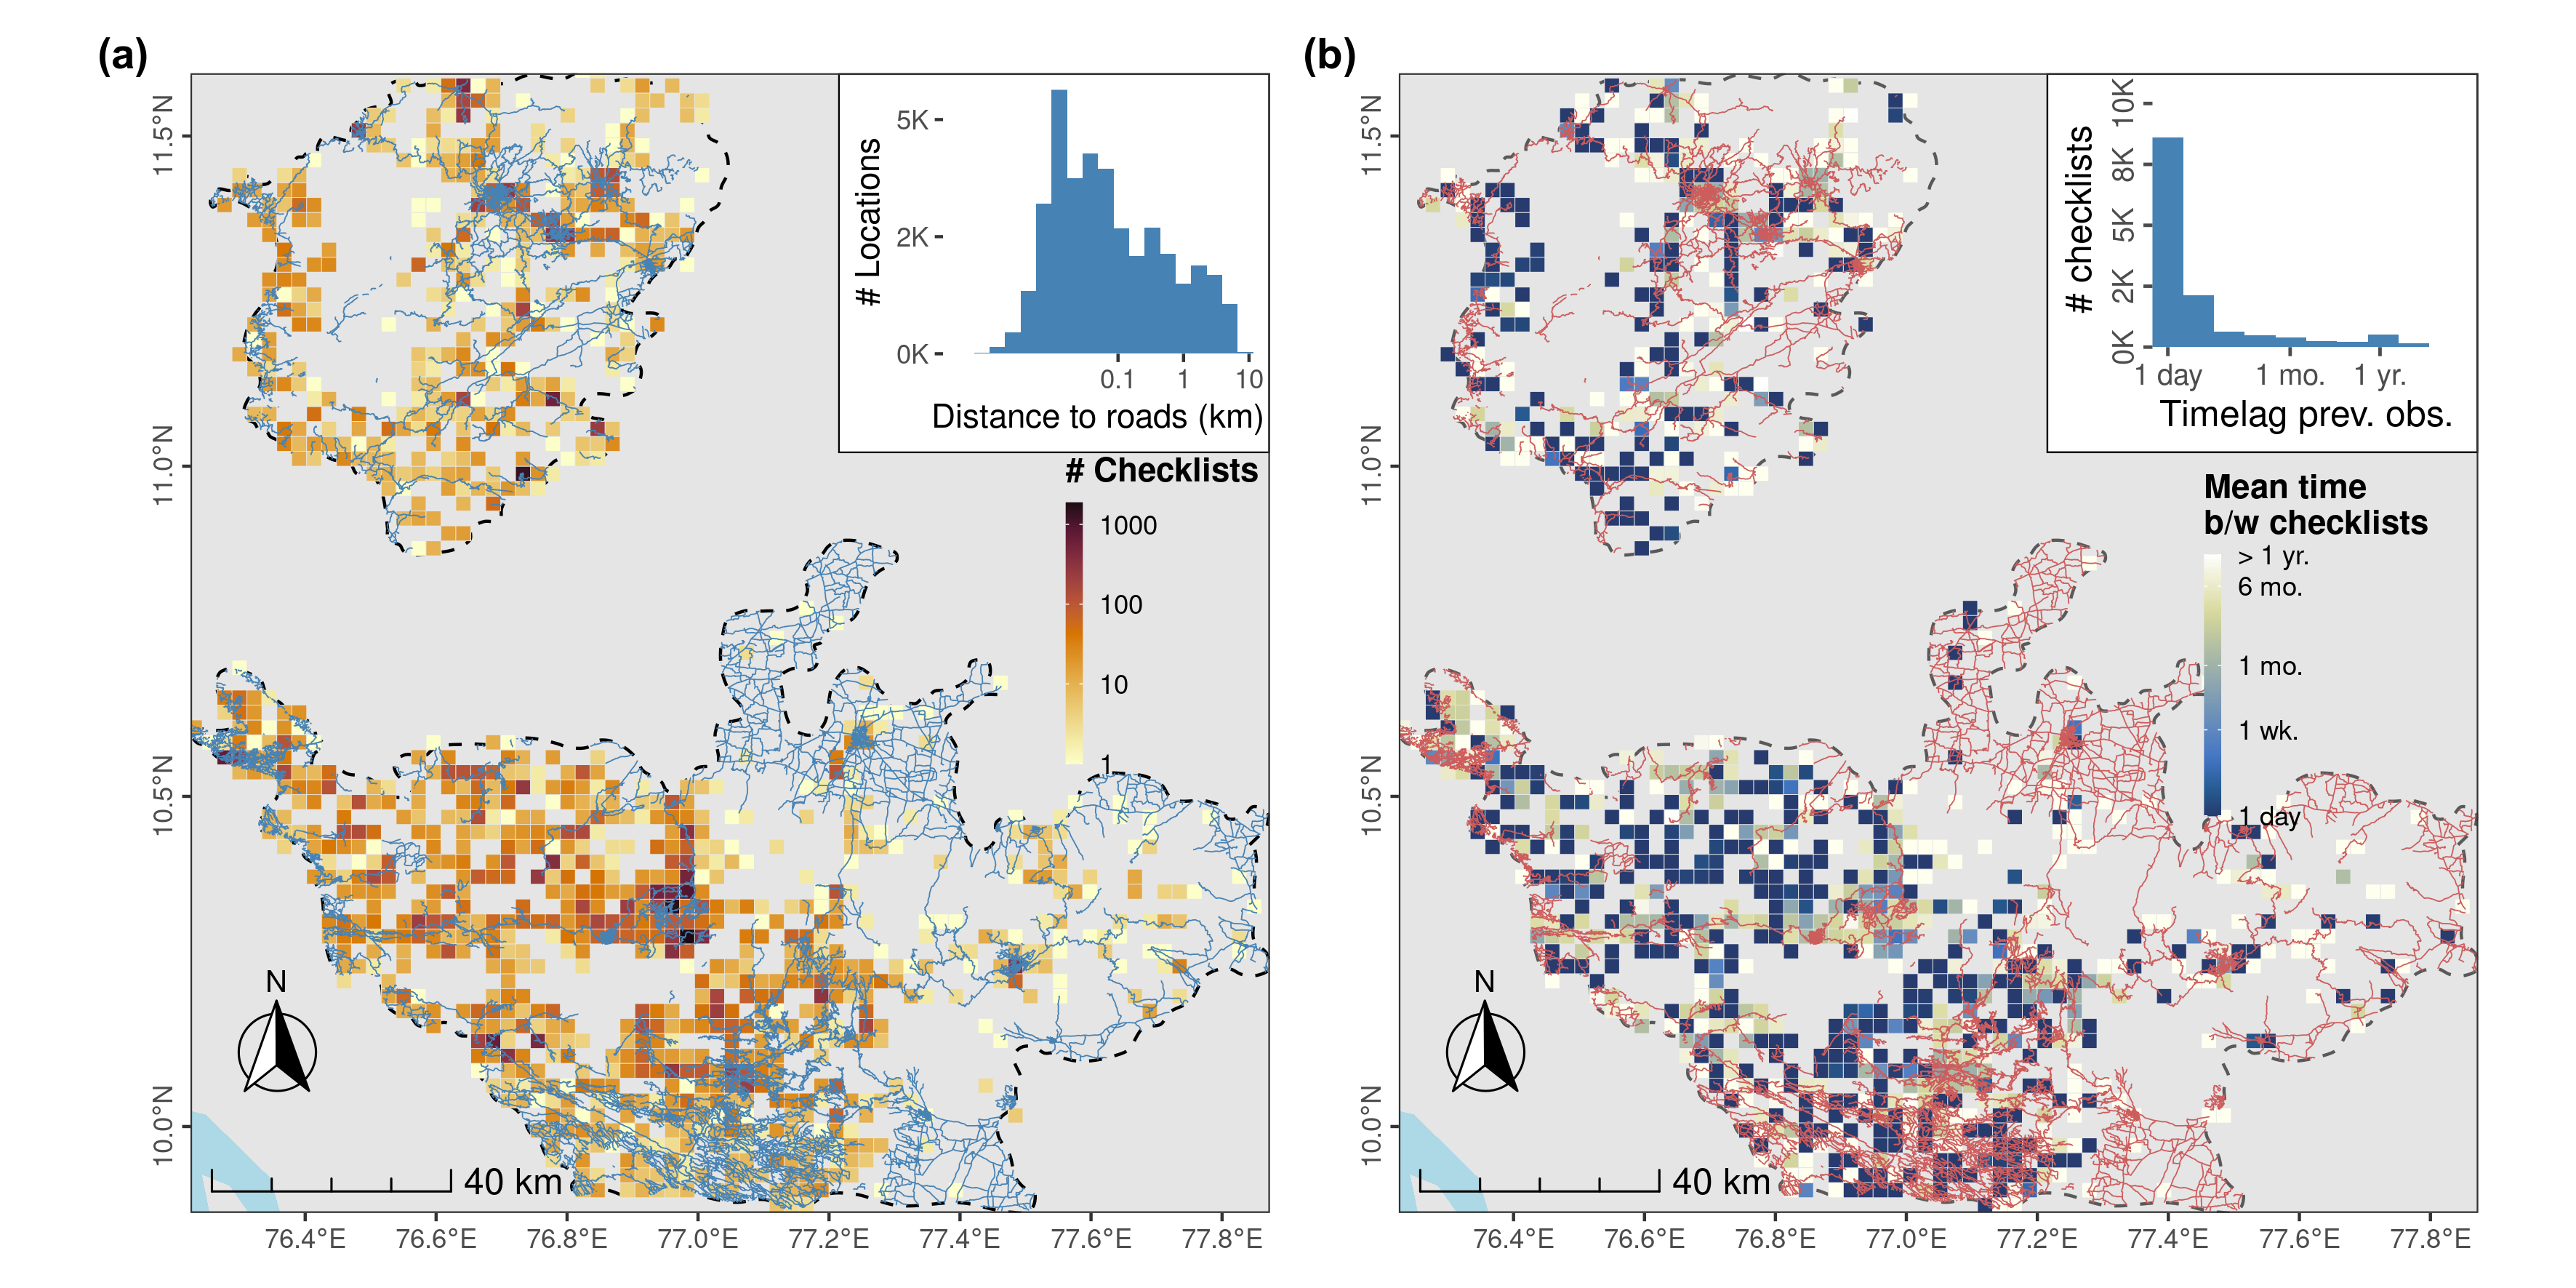
\includegraphics[width=0.9\textwidth]{figures/hillybirds/fig_03.png}
    \caption{
        \textbf{Distribution of sampling effort in the form of \textit{eBird} checklists in the Nilgiri and Anamalai Hills between 2013 and 2021.}
        \textbf{(a)} Sampling effort across the Nilgiri and Anamalai Hills, in the form of \textit{eBird} checklists reported by birdwatchers, mostly takes place along roads, with the majority of checklists located $<$ 1 km from a roadway (see distribution in inset), and therefore, only about 300m, on average, from the location of another checklist.
        \textbf{(b)} \textit{eBird} checklists are also strongly clustered in time, with some of the most sampled areas over the study period visited at intervals of $>$ 1 week, and with some less intensively sampled areas visited frequently, at intervals of $<$ 1 week.
        Overall, most checklists are reported only a day after the previous checklist at that location (see inset).
        Both spatial and temporal clustering make data thinning necessary.
        Both panels show counts or mean intervals in a 2.5 km grid cell; the study area is bounded by a dashed line, and roads within it are shown as (a) blue or (b) red lines.
    }
    \label{hilly_fig_03}
\end{figure}

\subsubsection*{Adjusting for Spatial Precision}

Every checklist on \textit{eBird} is associated with a latitude and longitude.
However, the coordinates entered by an observer may not accurately depict the location at which a species is detected.
Such an error can occur for two reasons: first, traveling checklists are associated with a single location along the route travelled by observers.
Second, checklist locations could be assigned to a `hotspot' --- a location that is automatically marked by \textit{eBird} as being frequented by multiple observers --- even though the observation was not made at the precise location of the hotspot \citep{praveenj.2017}.
Since a large proportion of observations occur within 3 km of the observation effort's starting point, we adjusted for the spatial precision of \textit{eBird} records by considering a buffer radius of 2.5km around each site when sampling environmental covariate values.

\subsubsection*{Calibrating Observations Across Observers}

Differences in bird identification skills among citizen scientists can lead to biased species detection when compared with data collected by a consistent set of trained observers \citep{vanstrien2013}.
Including observer calibration (that accounts for observer-specific differences in identification) as a detection covariate in occupancy models using \textit{eBird} data can help account for this variation \citep{johnston2018}.
Observer-specific calibration in local avifauna was calculated following \textcite{kelling2015a} as the normalized predicted number of species reported by an observer after 60 minutes of sampling across the most common land cover type within the study area (in our case, deciduous forests).
This score was calculated by examining checklists from anonymized observers across the study area.
We modified the \citep{kelling2015a} formulation by including only observations of the 79 species of interest in our calculations.
An observer with a higher number of species of interest reported within 60 minutes would have a higher observer-specific calibration score, with respect to the study area.
We then estimated a checklist calibration index (CCI) from observer-specific calibration scores associated with each checklist.
The CCI was the lone observer's calibration score for single-observer checklists and the highest calibration score among observers for group checklists.
CCI is predicted from a generalized linear mixed effects model:
\begin{multline*}
    \text{n} \sim \text{duration} + \sqrt{\text{duration}} + \text{landcover} + \sqrt{\text{time of day}} + \sqrt{\text{time of day}}^2 + \\ \log({\text{julian date})} + \log({\text{julian date})}^2 + (1 | \text{observer}) + \\(0 + \text{duration} | \text{observer})
\end{multline*}
where, $n$ is the number of species observed in that checklist, \textit{duration} is the time spent observing birds for the checklist, \textit{landcover} refers to the land cover type, \textit{time\_of\_day} refers to the time of the day that observations were made, and \textit{julian\_date} refers to the ordinal day of the year.

\subsubsection*{Preparing Occupancy Predictors}

We prepared a suite of climatic and land cover variables to be modeled as covariates of species-specific probabilities of occupancy within our full study region (Figs.~\ref{hilly_fig_01} 1 -- \ref{hilly_fig_02}).
Among climatic predictors, we chose to examine the effects of temperature and precipitation seasonality on species occupancy, and we obtained these predictors at a spatial scale of 1km \citep[Climatologies at High resolution for the Earth's Land Surface Areas; CHELSA:][]{karger2017}.
Temperature seasonality is defined as the amount of temperature variation over a given time period based on the ratio of the standard deviation of the monthly mean temperatures to the mean of the monthly temperatures \citep{odonnell2012}.
In other words, temperature seasonality is the coefficient of variation and captures the dispersion in relative terms because standard deviation can produce two similar values while the means may be different.
Larger values of temperature seasonality imply higher variability in temperature, relative to the average temperature.
It is important to calculate variability relative to the mean because the same amount of statistical variability (e.g., variance) in a dry area as a wet area would have a much bigger `seasonality' impact on a dry area.
Similarly, we defined precipitation seasonality as the ratio of the standard deviation of the monthly total precipitation to the mean monthly total precipitation \citep{odonnell2012}.
The above calculations of seasonality were made using temperature and precipitation data from CHELSA for the non-monsoon months of December to May for our study area.
While data from global databases such as WorldClim have been used for modeling species distributions, CHELSA data has shown greater predictive power \citep{karger2017} and hence we used the latter in this study.
Other bioclimatic predictors such as mean annual temperature, mean annual precipitation, mean temperature of the coldest or driest quarter, or the precipitation of driest or coldest quarter were equally well suited for our study; however, they were highly correlated ($|r|$ $>$ 0.5) with temperature and precipitation seasonality.
We obtained land cover over our study site from a high-resolution vegetation type map generated by \citep{roy2015}, using medium resolution IRS-LISS III (Indian Remote Sensing Satellite - Linear Imaging Self Scanner) images (http://bis.iirs.gov.in/).
This classification was originally generated at a scale of $\sim$23m and with 22 land cover classes for our study area.
We aggregated these 22 classes into seven broad, ecologically relevant land cover types: evergreen forests, deciduous forests, mixed/degraded forests, agriculture/settlements, plantations, grasslands, and water bodies (see Supplementary Material).
We resampled the reclassified land cover layer using a nearest neighborhood approach to 1km to match the 1km resolution of the climatic layers.

Testing for collinearity among the climatic and land cover predictors did not result in the removal of any predictors as the correlations were low ($|r| <$ 0.5).
We then pooled the climatic (n = 2) and land cover (n = 7) predictors and calculated mean values for the two climatic predictors (temperature seasonality and precipitation seasonality) and calculated the proportion of each of the seven land cover types within the 2.5km buffer radius around each spatio-temporally thinned locality for each species.

\subsubsection*{Estimating Species Occupancy}

Occupancy models estimate the probability of occurrence of a given species while controlling for imperfect detection and allow us to model the factors affecting occurrence and detection independently \citep{mackenzie2017,johnston2018}.
The flexible \textit{eBird} observation process contributes to the largest source of variation in the likelihood of detecting a particular species \citep{johnston2021}; hence, we included six continuous covariates that influence the probability of detection for each checklist: ordinal day of year, duration of observation, distance travelled, time of day of observations, number of observers, and the checklist calibration index (CCI).
We converted calendar date into a linear, continuous predictor by extracting ordinal days of the year (julian date) for December to May and scaling them between 1 and 183 (dates in December subtracted from 333, and 31 added to dates between January and May).
This time period essentially includes winter and summer seasons (loosely defined) in the Western Ghats where detectability of bird species is high.
Our breeding season is often toward the end of this window (late April to early May) when resident species begin to breed while migratory birds travel back to their breeding grounds.
We modeled time of day so as to allow detectability to be highest at dawn and dusk when birds often sing and are easily detected, and to be lower in the middle of the day, when birds are least active and thus less likely to be detected.

Using a multi-model information-theoretic approach, we tested how strongly our occurrence data fit our candidate set of environmental covariates \citep{burnham2002}.
We fitted single-species occupancy models for each species, to simultaneously estimate a probability of detection ($p$) and a probability of occupancy ($\psi$) \citep{mackenzie2002,fiske2011}.
For each species, we fit 512 models, each with a unique combination of the (climate and land cover) occupancy covariates and all detection covariates (the six detection covariates are present in every model).

\begin{multline*}
    \text{logit}(p) \sim \text{julian date} + \text{duration} + \text{distance} + \text{obs. started} + \\
    \text{number observers} + CCI    
\end{multline*}

where \textit{julian date} refers to the ordinal day of the year, \textit{duration} refers to the time spent observing birds in minutes, \textit{distance} is the distance travelled by the observer(s) in kilometers, \textit{obs. started} is the time of day when observations were recorded, \textit{number observers} refer to the number of observers, and $CCI$ is the checklist calibration index.

\begin{multline*}
    \text{logit}(\psi) \sim \text{BIO 4a} + \text{BIO 15} + p(\text{Evergreen}) + p(\text{Deciduous}) + \\
    p(\text{MixedDegraded}) + p(\text{AgricultureSettlements}) + p(\text{Plantations}) + \\
    p(\text{Grasslands}) + p(\text{WaterBodies})
\end{multline*}

Previously, we explored the non-linear effects of temperature seasonality and precipitation seasonality.
However, our occupancy models showed a poor fit to the data when temperature and precipitation seasonality were included as non-linear terms and hence, we did not explore this further.
Adequate model fit was assessed using a chi-square goodness-of-fit test using 1,000 parametric bootstrap simulations on a global model that included all occupancy and detection covariates (MacKenzie and Bailey 2004).
Across the 512 models tested for each species, the model with highest support was determined using AICc scores.
However, across the majority of the species, no single model had overwhelming support.
Hence, for each species, we examined those top models which had a difference in AICc of $<$ 4, as these top models were considered to explain a large proportion of the association between the species-specific probability of occupancy and environmental drivers \citep{burnham2011}.
Using these restricted model sets for each species; we created a model-averaged coefficient estimate for each predictor and assessed its direction and significance \citep{barton2009}.
These model-averaged coefficients include zeros when a predictor is absent in one of the top models.
In addition, we estimated a model-averaged standard error using which we calculated a 95\% confidence interval \citep{burnham2002}.
We considered a predictor to be significantly associated with occupancy if the range of the 95\% confidence interval around the model-averaged coefficient did not contain zero.

Prior to further inference, all 79 birds in our study were classified as forest species or generalist species following \citep{ali1983}.
Forest species are those that are typically found in wet evergreen, semi-evergreen, deciduous, moist deciduous forests, and other woodland habitats as well as forest edges.
This classification encompasses specialist endemic birds, species that occur in woodland habitats as well as those species found along the edges of forested areas.
Generalist species are those that are typically found across a range of habitat types such as forests, agricultural lands, settlements, etc.

All continuous covariates were standardized prior to analysis, allowing for the comparison of model-averaged coefficients between species.
We used the R packages unmarked, and MuMIn for occupancy modeling and model averaging; the code provided in the supplementary material and on our Github repository shows the full set of R and Python packages used in this work \citep{barton2009,fiske2011,r2020}.

\subsubsection*{Data deposition}

All data were downloaded from \textit{eBird} (version 1.13) and can be accessed via: http://\textit{eBird}.org/data/download.
The complete analysis is available as Supplementary Material (https://github.com/vjjan91/\textit{eBird}Occupancy) and is archived on Zenodo (https://doi.org/10.5281/zenodo.6025640).

\section*{Results}

Following spatio-temporal thinning of observations, we relied on 315,428 curated citizen scientist observations (including both presences and non-detections) across 79 species of birds between 2013 and 2021 for modeling occupancy.
The number of detections varied from a minimum of 224 observations to a maximum of 7,725 observations per species (following spatio-temporal thinning).
Chi-square goodness-of-fit tests suggested a poor model fit for twenty-four species ($p <$ 0.05; Appendix S2) and hence these species were removed before further analysis (resulting in a total of 55 species).
Of the list of 55 species, six species were migratory species (long-distance/altitudinal) that are present in our study area during the focal seasonal time period: Blyth's reed warbler \textit{Acrocephalus dumetorum}, Brown shrike \textit{Lanius cristatus}, Chestnut-headed bee-eater \textit{Merops leschenaulti}, Grey wagtail \textit{Motacilla cinerea}, Eurasian hoopoe \textit{Upupa epops} and Ashy drongo \textit{Dicrurus leucophaeus}.

\subsubsection*{Bird-climate associations}

The probability of occupancy of $\sim$78\% (n = 43 out of 55) of species examined was significantly ($p <$ 0.05) associated with temperature seasonality.
18 bird species (n = 14 generalist birds and 4 forest birds) showed a positive association with temperature seasonality, while 25 bird species (n = 7 generalist birds and 18 forest birds) were negatively associated (Fig.~\ref{hilly_fig_04}; Table 1).
The probability of occupancy of $\sim$38\% of (n = 21 out of 55) species examined had a significant association with precipitation seasonality.
14 bird species (n = 8 generalist birds and 6 forest birds) showed a positive association, while seven bird species (n = 5 generalist birds and 2 forest birds) were negatively associated with precipitation seasonality.

\begin{figure}[h!]
    \centering
    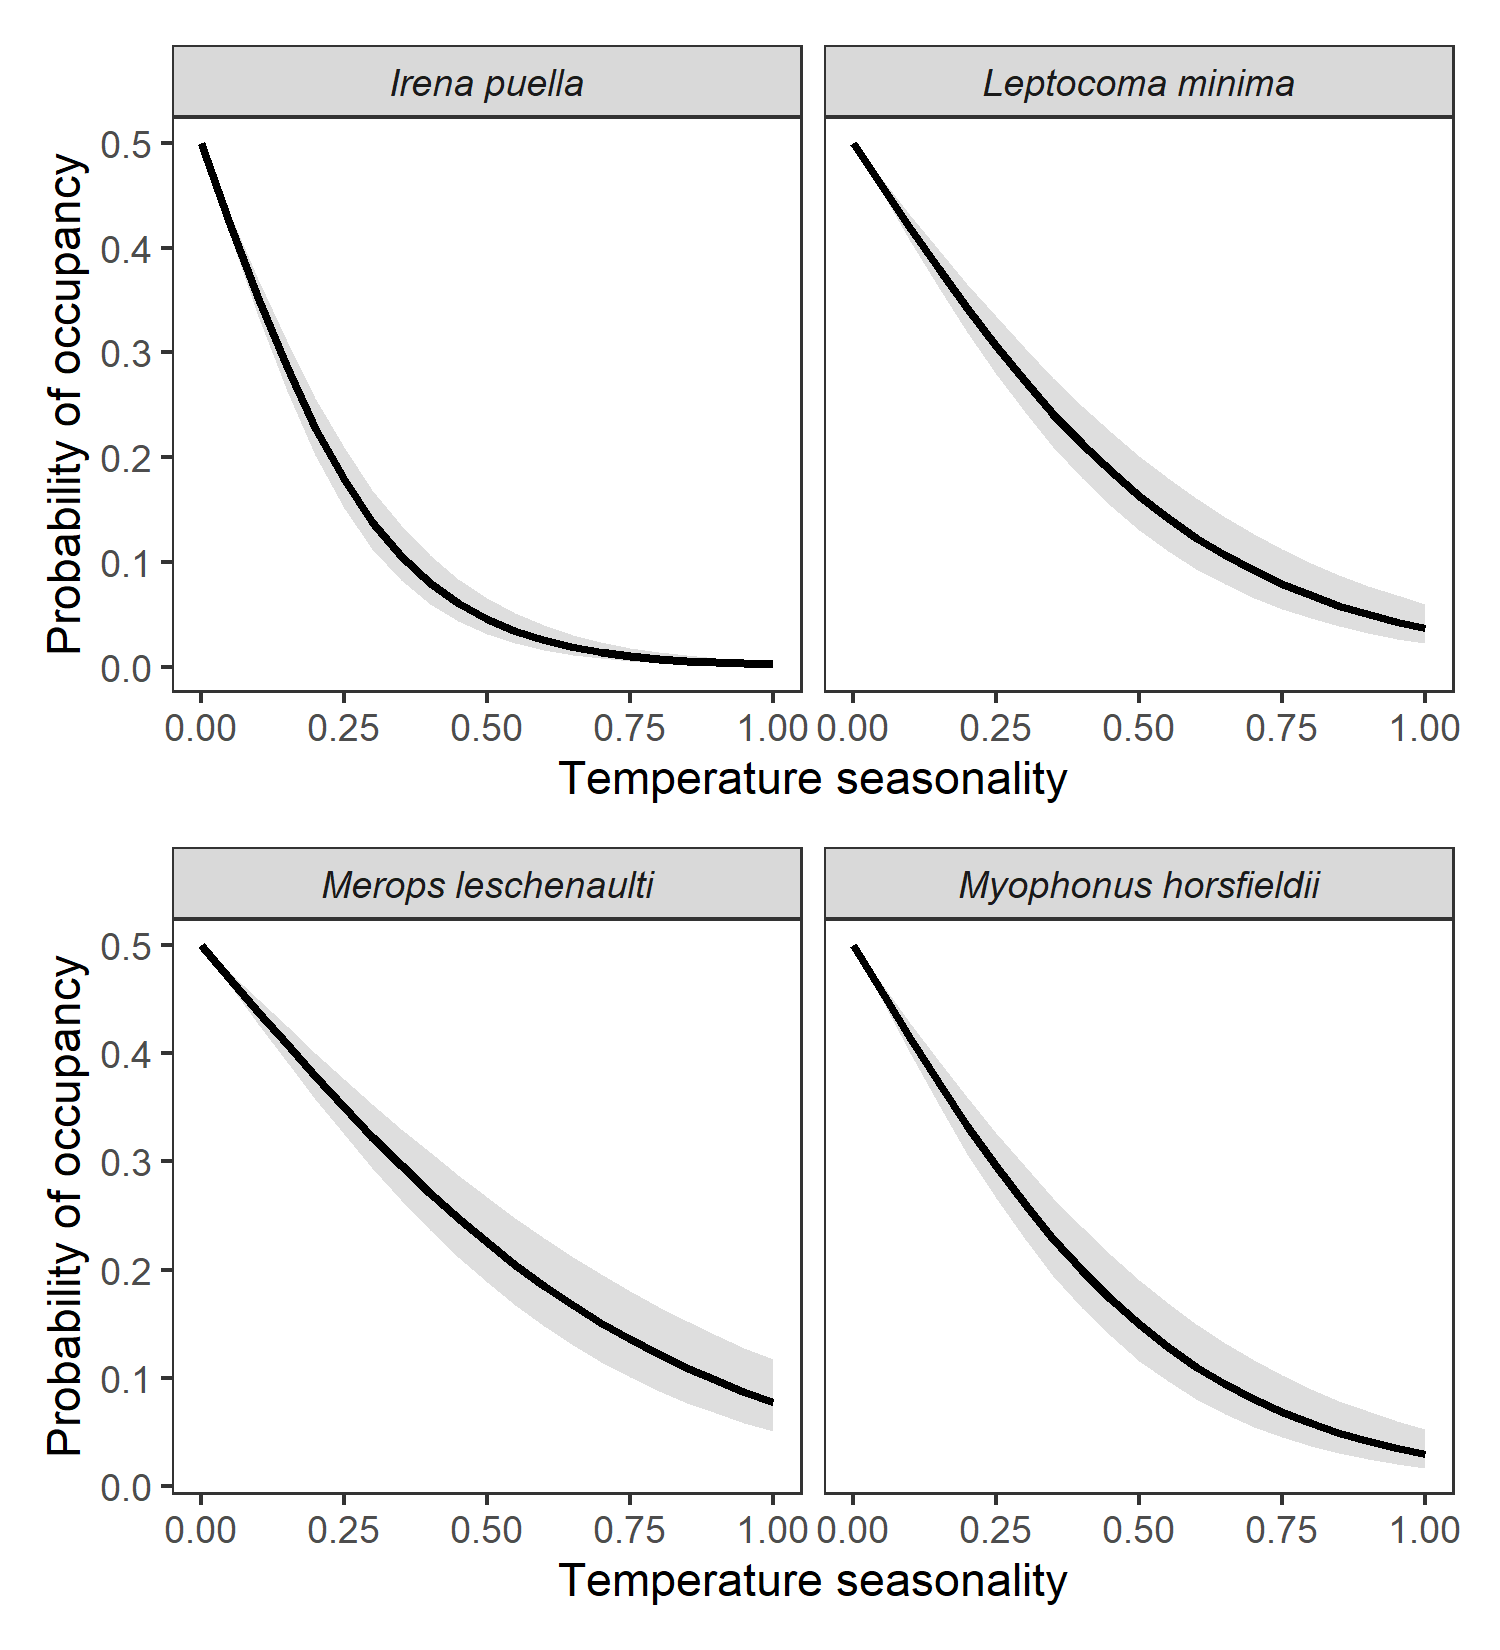
\includegraphics[width=0.9\textwidth]{figures/hillybirds/fig_05.png}
    \caption{
        \textbf{Probability of occupancy as a function of temperature seasonality.}
        Predicted probability of occupancy curves as a function of temperature seasonality for four forest species are shown here. 
        Temperature seasonality is negatively associated with the probability of occupancy of several forest species including the Asian fairy-blu\textit{eBird} (\textit{Irena puella}), the crimson-backed sunbird (\textit{Leptocoma minima}), the chestnut-headed bee-eater (\textit{Merops leschenaulti}) and the Malabar whistling-thrush (\textit{Myophonus horsfieldii}).
    }
    \label{hilly_fig_05}
\end{figure}

\begin{figure}[h!]
    \centering
    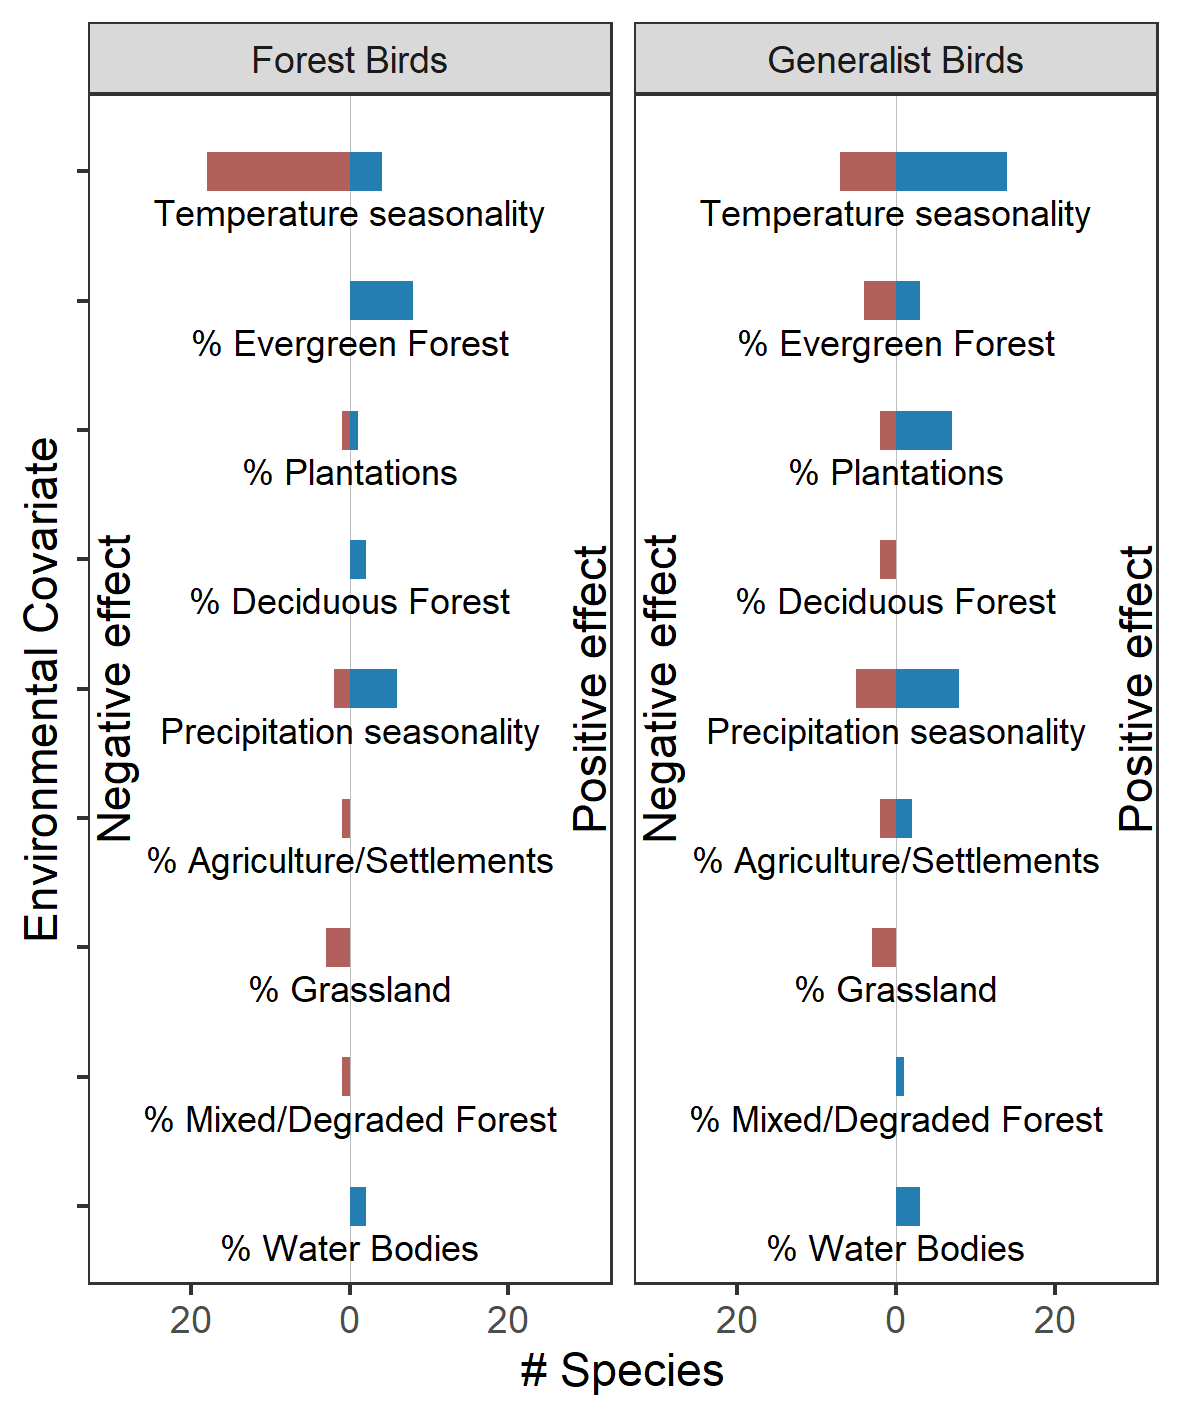
\includegraphics[width=0.9\textwidth]{figures/hillybirds/fig_04.png}
    \caption{
        \textbf{Environmental predictors and species-specific associations}.
        The direction of association between species-specific probability of occupancy and climatic and landscape predictors is shown here (as a function of habitat preference). 
        Blue colors show the number of species that are positively associated with a climatic/landscape predictor while red colors show the number of species that are negatively associated with a climatic/landscape predictor (see Table 1 for the number of forest/generalist species that show positive/negative association with each of the predictors).
    }
    \label{hilly_fig_04}
\end{figure}

\subsubsection*{Bird-land cover associations}

Twenty-seven percent of species (n = 15 out of 55) were significantly associated with the proportion of evergreen forests.
Of these species, eight forest birds were positively associated.
Among generalist birds that showed a significant association with the proportion of evergreen forests, three species were positively associated while four were negatively associated.
A fewer number of species (n = 4) were significantly associated with the proportion of deciduous forests (positive association with two forest species and a negative association with two generalist bird species).
Six bird species showed a significant association with the proportion of grasslands.
Of these species, three forest bird species and three generalist birds showed a negative association (Fig.~\ref{hilly_fig_04}; Table 1).
Five bird species were significantly and positively associated with the proportion of water bodies (n = 3 generalist birds and 2 forest birds).

\begin{figure}[h!]
    \centering
    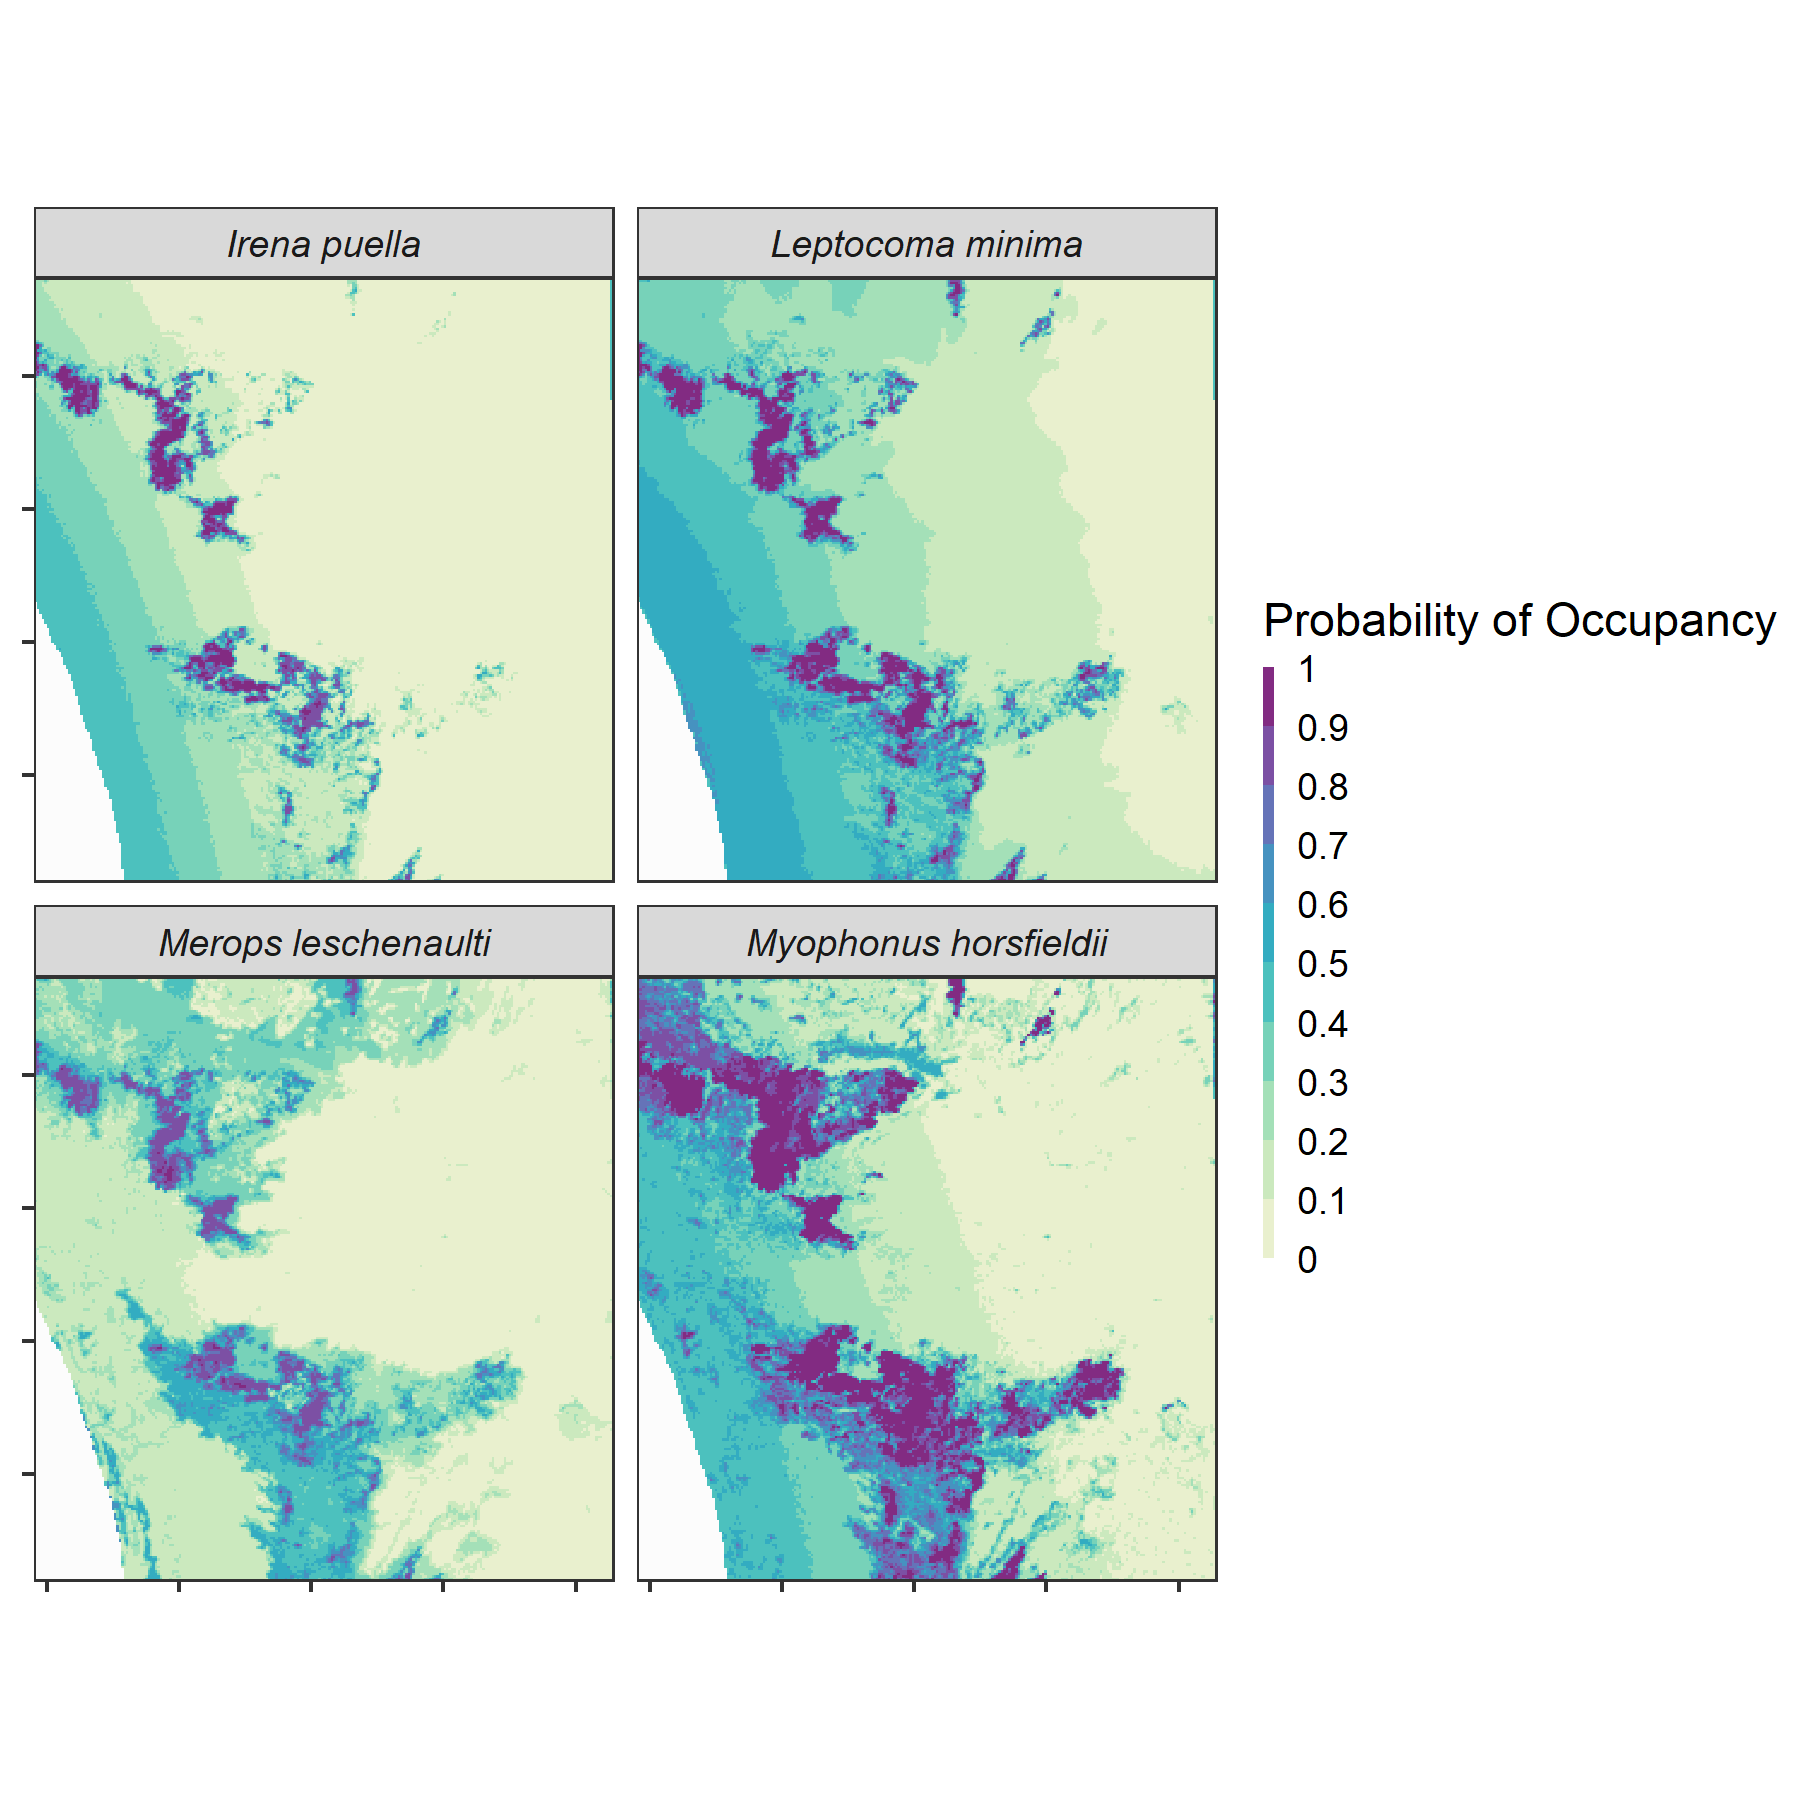
\includegraphics[width=0.9\textwidth]{figures/hillybirds/fig_06.png}
    \caption{
        \textbf{Predicted area of occurrence for four forest species.} 
        The probability of occupancy of the Asian fairy-blu\textit{eBird} (\textit{Irena puella}), the crimson-backed sunbird (\textit{Leptocoma minima}) and the chestnut-headed bee-eater (\textit{Merops leschenaulti}) is higher across the western slopes and at mid-elevations across our study area. The Malabar whistling-thrush (\textit{Myophonus horsfieldii}) has a higher probability of occupancy across mid-elevations throughout the study area examined.
    }
    \label{hilly_fig_06}
\end{figure}

33\% (n = 18 out of 55) of species examined were significantly associated with human-modified land cover types --- including the proportion of agriculture or settlements, plantations, and mixed or degraded forests.
One forest species showed a negative association, and one generalist species was positively associated with the proportion of mixed or degraded forests.
Five bird species showed a significant association with the proportion of agriculture or settlements.
Of these species, two generalist bird species showed a positive association while one forest species and two generalist bird species showed a negative association.

Eleven bird species showed a significant association with the proportion of plantations.
Of these species, one forest bird species showed a negative association, and one forest bird species showed a positive association.
Among generalist birds that showed a significant association with the proportion of plantations, seven birds were positively associated while two birds showed a negative association.

\section*{Discussion}

Our study shows that rigorously filtered and curated citizen science observations can be used within a robust statistical framework to inform our understanding of how environmental drivers are associated with species distributions.
We highlight the role of climate and land cover and its associations with bird occurrences along a tropical montane gradient in a biodiversity hotspot, the southern Western Ghats.

\subsubsection*{The role of temperature}

Tropical montane birds are especially vulnerable to ongoing changes in climate \citep{sekercioglu2007,perez2016,freeman2018,srinivasan2018}.
As a result of reduced temperature seasonality in the tropics relative to temperate regions, montane species in particular exhibit narrow thermal niches and hence, are likely to be unable to shift their distributions to track future climate changes \citep{janzen1967,deutsch2008,tewksbury2008,jankowski2013}.
Previous work in tropical areas across the globe have demonstrated that forest species are adapted to thermally aseasonal environments, while generalist species are more adapted to thermally variable, seasonal environments \citep{frishkoff2016,chan2016}.
In line with previous work, our study showed that several forest bird species (n = 18) were negatively associated with temperature seasonality.
Species such as the crimson-backed sunbird \textit{Leptocoma minima}, Asian fairy-blu\textit{eBird} \textit{Irena puella} and the chestnut-headed bee-eater \textit{Merops leschenaulti} for example showed a negative association (Fig.~\ref{hilly_fig_05}; Fig.~\ref{hilly_fig_06}).
The above result suggests that forest birds across the elevational gradient are potentially associated with narrow thermal niches.
Similar results have been demonstrated in the Western Himalayas, where birds occurring in forested habitats have narrow thermal niches relative to species in other land cover types \citep{srinivasan2019}.

In line with our hypothesis, the probability of occupancy of several generalist bird species (n = 14) was positively associated with temperature seasonality.
For example, the red-vented bulbul \textit{Pycnonotus cafer}, purple sunbird \textit{Cinnyris asiaticus}, and the spotted dove \textit{Streptopelia chinensis} showed a positive association.
Our result suggests that such generalist species occupy areas that show large variation in temperatures - including drier open habitats such as mixed or degraded forests and agricultural lands.
In fact, temperatures across tropical agricultural lands have been shown to be 7.6℃ higher than temperatures within tropical primary forests \citep{senior2017}.
Generalist bird species that showed a positive association likely possess broad thermal niches, relative to their forest counterparts.
However, our study also reported a negative relationship with temperature seasonality for seven generalist bird species, including the red-whiskered bulbul \textit{Pycnonotus jocosus} and the Oriental magpie-robin \textit{Copsychus saularis}.
Future studies need to consider climate-land cover interactions to explore patterns seen for generalist species.

\paragraph*{The role of precipitation}

The significant association with precipitation seasonality suggests the importance of the `hygric niche', which has been seldom explored empirically \citep{boyle2020}.
In other words, species' occupancy is often governed by a range of precipitation regimes which vary in turn by land cover type and topographic complexity \citep{nowakowski2018}.
Several forest and generalist species showed a positive association with precipitation seasonality.
Research from the Australian tropical rainforests suggests that precipitation seasonality was strongly associated with bird abundance \citep{williams2008}.
In addition, precipitation seasonality has been reported as a crucial factor influencing resource availability (e.g., insects) for bird populations \citep{loiselle1991}.
The positive association between precipitation seasonality and species occupancy (for forest and generalist birds) reported in this study can be explained by the cascading effect of rainfall on food availability and, thereby survival of birds \citep{butt2015,boyle2020}.
In our study, forest species such as the southern hill myna \textit{Gracula indica} and the crimson-backed sunbird \textit{Leptocoma minima}, and generalist species such as the rose-ringed parakeet \textit{Psittacula krameri} and the Indian white-eye \textit{Zosterops palpebrosus} showed a positive association.
On the other hand, we found that generalist species like the coppersmith barbet \textit{Psilopogon haemacephalus} and the red-vented bulbul \textit{Pycnonotus cafer} were negatively associated with precipitation seasonality.
Many of these generalist bird species that showed a negative association is associated with drier habitats across our study area.
Similar results have been reported from the neotropics where bird species largely associated with open habitats tend to prefer drier climates \citep{frishkoff2016}.
The above result merits further exploration that tests the interaction between precipitation seasonality and habitat structure and floristics in determining habitat use.
With increasing variability in rainfall patterns, it remains to be seen whether forest, as well as generalist bird species, adapt to such changes in the near future.
For instance, models have predicted reduced rainfall across regions in the Western Ghats as a result of future climatic changes \citep{rajendran2012}.

\subsubsection*{Role of naturally occurring vegetation and landscape transformation}

Apart from climate, certain land cover types are hypothesized to be crucial for many species, as they offer resources necessary for survival, breeding, and other activities \citep{sunarto2012}.
For insectivorous birds in central Jamaica, the landscape matrix and habitat type were vital in determining occupancy \citep{kennedy2011}.
Our study suggests a positive relationship for several forest species across naturally occurring land cover types --- evergreen and deciduous forests.
Few generalist species such as the Blyth's reed warbler \textit{Acrocephalus dumetorum} and gray wagtail \textit{Motacilla cinerea} were positively associated with the proportion of evergreen forests.
The above association can be attributed to the fact that the Blyth's reed warbler and the gray wagtail have been reported from forest edges as well as plantations and agricultural areas in the vicinity of evergreen forests.
It is also likely that our minimum spatial scale of 2.5km was coarse and resulted in sampling multiple land cover types.

As expected, several generalist bird species showed a positive association with human-modified land cover types.
This association highlights the role of habitat transformation.
The southern Western Ghats have undergone a drastic transformation in the last two decades, with the replacement of mid- and high-elevation forests and grasslands with exotic trees and plantations \citep{arasumani2018}.
In the Nilgiris alone, the area covered by exotic trees has almost doubled, from approx.
140 sq. km to 277 sq. km in the 44-year period between 1973 and 2017.
Generalist birds such as the jungle myna \textit{Acridotheres fuscus} and the red-whiskered bulbul \textit{Pycnonotus jocosus} were positively associated with the proportion of plantations.
On the other hand, we did see forest species like the Malabar whistling thrush \textit{Myophonus horsfieldii} showing a positive association with the proportion of plantations, which could be an artifact of this species often being reported in not only forested areas but forest edges and plantations as well.
In a complex matrix that is the Western Ghats, our results further lend support to the role of natural vegetation within these human-modified landscapes in sustaining biodiversity in the long term \citep{anand2010,ranganathan2010}.
For example, windbreaks, which are often thin slivers of natural vegetation present in tea plantations in our study area, have been shown to possess similar bird species richness compared to adjacent primary forests \citep{sreekar2013}.
In a similar vein, data from the Anamalai hills suggests that native shade trees within tea plantations bolster avian species richness almost two-fold compared to tea plantations without native shade trees \citep{raman2021}.
Furthermore, the type of human-modified land cover type matters too, and coffee, rubber, and areca plantations across the Western Ghats have been shown to support more bird species than tea plantations \citep{sidhu2010,karanth2016}.

\subsubsection*{Caveats and Conclusions}

Our analysis was carried out using semi-structured data derived from a large citizen science project.
The lack of experimental and sampling design of this study is a persistent criticism of citizen science research.
For example, a large proportion of checklists were reported within 200m of a road, which are relatively more accessible (Fig.~\ref{hilly_fig_03}a).
This pervasive spatial bias in sampling could impact results in ways that cannot be corrected via spatio-temporal filtering of data.
While citizen science observations are often seen as supplementary to (presumably) more rigorous, methodical sampling by trained observers, such sampling designs are often not logistically feasible at large spatial scales.
In under-studied or under-sampled regions, citizen scientists and their observations are first-class data sources with significant exploratory and explanatory power \citep{devictor2010,ellwood2017,robinson2020}.

Recent evidence also suggests that a species' response to environmental gradients or to drivers such as land cover and climate will vary as a function of biological traits \citep{mcgill2006}.
Our study classified species as forest species or generalist species \citep{ali1983}.
Other traits might better explain associations between climatic and land cover predictors and species' occupancy.
For example, body mass is often considered an indicator of thermoregulation, and has been shown to be strongly associated with thermal niches of species, particularly temperate species, and high elevation tropical species \citep{barve2021}.
Similarly, functional traits such as trophic niches, that explain dietary preferences of a particular species are often associated with the use of a particular habitat \citep{pigot2020}.
Himalayan birds --- which encounter a comparable, if wider, range of temperatures --- have been shown to use forest and agriculture habitats to cope with resource scarcity in winter, possibly indicating greater dietary generalization than previously thought \citep{elsen2018}.
Including functional traits is a promising avenue to better understand species' response to environmental change across human-modified landscapes in the Western Ghats, and tropical mountains more generally.

Over 60\% of mountainous landscapes across the planet are under tremendous anthropogenic pressures, and yet host some of the highest biodiversity in the world \citep{lasorte2010,elsen2020}.
The southern Western Ghats is one such human-dominated mountainous landscape, where understanding the role of climatic and landscape predictors in structuring species occupancy can inform conservation.
In this study, we show that species have differential responses to climate (temperature and precipitation) and natural and human-modified land cover types.
If species need to adapt to environmental changes, they need to be able to track their suitable climatic and habitat niche space, which may only be possible through the creation of climate corridors \citep{freeman2018}.

\newrefcontext[sorting=nyt]
\printbibliography[title=Literature~Cited,sorting=nyt,heading=subbibliography]


\clearpage \cleardoublepage
\begin{interludeenv}

\begin{refsection}
\newrefcontext[sorting=ynt]
% \addtocontents{toc}{\protect\vspace{\beforebibskip}}%
%\chapter*{Mapping Animal Movement in \textit{R}: The Science and the Art}
%\chaptermark{Mapping Animal Movement in \textit{R}: The Science and the Art}
\phantomsection
\pagestyle{plain}
\pagecolor{Snow1}
% \begin{addmargin}[-2.0cm]{0cm}

	% \addcontentsline{toc}{chapter}{\tocEntry{\color{darkgray}{\adftripleflourishleft~~Box 3: Changes to environmental rules are associated with an increase in forest clearance proposals}}}%
	\interlude{Environmental Governance in India}\label{box:clearances}

	\noindent Vijay Ramesh\textsuperscript{1}, \textbf{Pratik R. Gupte}, and Mridula M. Paul\textsuperscript{2}

	\marginpar{
	    \textsuperscript{1} Columbia University, USA.
	    
	    \medskip
	    
	    \textsuperscript{2} Ashoka Trust for Research in Ecology and the Environment, India.
	}

	\medskip
	\footnotesize

	\noindent {{$\Delta$}} {\footnotesize This box is adapted from an article written in response to the publication of the Draft Environmental Impact Assessment (EIA) Rules, 2020, in India --- only one among a spate of efforts worldwide to use the Covid-19 pandemic as cover for sweeping changes to regulations in environmental policy and civil liberties.
	The article appeared online in \textit{Sanctuary Asia}.}

	\medskip

	Environmental Impact Assessments (EIA) are crucial to balance environmental imperatives with economic development.  
	In March 2020, the Government of India's Ministry of Environment, Forest and Climate Change (MoEFCC) published a revised draft Environmental Impact Assessment (EIA) Notification, titled Draft EIA 2020, to make the process of granting project approval more standardized and transparent (1). 
	Environmentalists nationwide have voiced significant concerns with respect to this draft, citing considerable dilution of existing EIA regulations (2). 

	The EIA Notification was initially issued in 1994 (3), and further revised by ministerial notification in 2006 (4). 
	Analysis of MoEFCC forest clearance data (5) between 1994 and 2019 shows that projects applied for significantly more forest area to be cleared in years when or shortly after a new EIA notification was adopted. 
	These years, 1995 and 2006, saw approximately 4,000 sq.km. and approximately 3,000 sq.km. respectively, proposed for clearance, which is nearly twice as much area proposed in other years (6). 
	Further, applications in 1995 and 2006 were just as successful as they were in other years, and thus 814\% more forest area was approved for clearance compared to other years (6).

	\begin{figure}[h!]
	    \centering
	    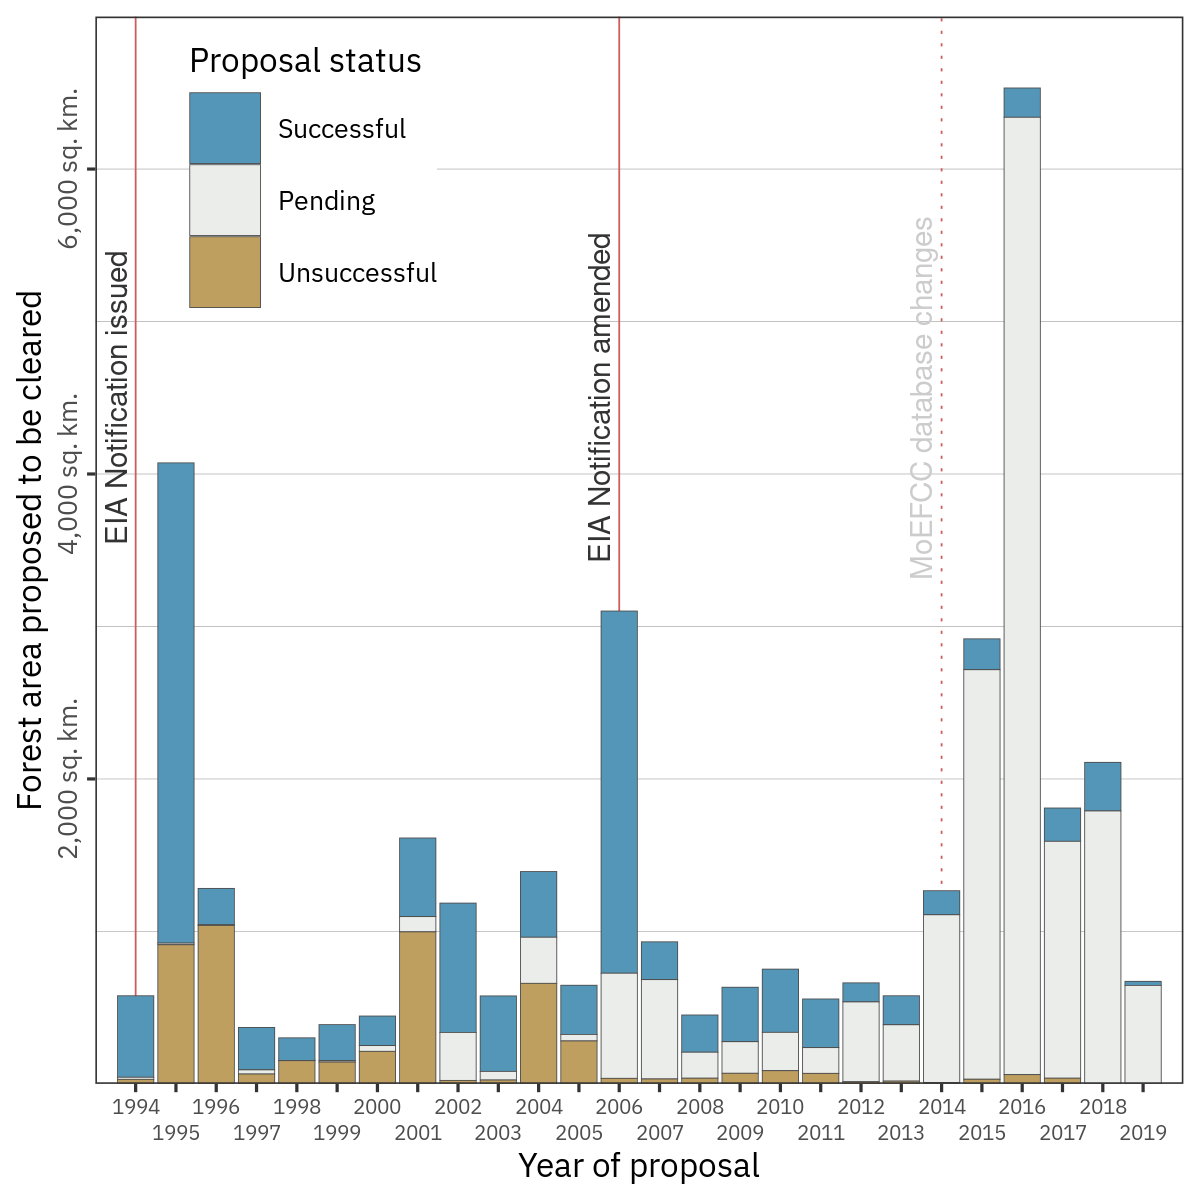
\includegraphics[width=0.7\textwidth]{figures/boxes/clearances.png}
	    \caption{
	        \textbf{Forest areas proposed to be cleared since the advent of environmental protections in India.} 
	        Forest area (in sq. km.) proposed for clearance over the years 1994 -- 2019, coloured to show the fraction approved (blue), rejected (brown), and pending decision (grey). Projects applied for nearly twice as much area to be cleared in years when or shortly after a new EIA notification was adopted (1995 and 2006), as in other years. Since the approval rate for projects did not differ significantly among years, 1995 and 2006 saw 814\% more forest area approved for clearance than other years.
	    }
	    \label{fig_box_clearances}
	\end{figure}

	Between 1994 and 2013, 70\% of forest area proposed for clearances was approved. 
	If this clearance rate were applied to forest clearances pending since 2014, India could see an additional 9,900 sq. km. of forest land cleared, about twice as much as in the preceding twenty years combined. 
	Provisions in the Draft EIA Rules, 2020, such as regularisation of environmental safeguards violations, or allowing projects to fence off forest land before the EIA process could cause further forest loss and degradation commensurate with 1995 and 2006. 
	MoEFCC must reconsider the Draft EIA Rules, 2020, and strengthen environmental governance if India is to meet national reforestation (7) and international climate targets (8).

\begin{enumerate}
	\item MoEFCC, “Draft Notification” (New Delhi, 2020).
	\item V. Chandrashekhar, India’s push to relax environmental assessment rules amid pandemic draws criticism. Science (80-. ). (2020), (available at https://www.sciencemag.org/news/2020/05/india-s-push-relax-environmental-assessment-rules-amid-pandemic-draws-criticism).
	\item MoEFCC, “The Environmental Impact Assessment Notification” (S.O.60(E), New Delhi, 1994).
	\item MoEFCC, “Environmental Impact Assessment Notification” (S.O.1533(E), New Delhi, 2006).
	\item PARIVESH: A Single Window Integrated System for Environment, Forest, Wildlife and CRZ Clearances, (available at https://parivesh.nic.in/).
	\item Pratik Rajan Gupte. (2020, July 2). Code for India forest clearance analyses (Version v1.0). Zenodo. http://doi.org/10.5281/zenodo.3925792.
	\item B. Borah, A. Bhattacharjee, N. Ishwar, “Bonn Challenge and India: Progress on restoration efforts across states and landscapes.” (New Delhi, 2018), (available at https://portals.iucn.org/library/sites/library/files/documents/2018-026-En.pdf).
	\item M. Aggarwal, India needs to double rate of forest cover expansion to achieve Paris Agreement target. Mongabay India (2019), (available at https://india.mongabay.com/2019/11/paris-agreement-goals-india-needs-to-double-forest-cover-expansion-rate/).
\end{enumerate}

% \end{addmargin}
\afterpage{\nopagecolor}
\pagestyle{scrheadings}

\end{interludeenv}

\clearpage \cleardoublepage
\ctparttext{Animal movement is neither random nor optimal, but the outcome of individuals making movement decisions based on local information. The strategies underlying these decisions are, like everything in biology, shaped by animals' evolutionary contexts. Yet evolution is rarely considered in animal movement models, possibly because it is considered to be too slow to be relevant to outcomes on human timescales. 

In the second part of this thesis, I probe the evolution of animal movement, and show how evolutionary shifts in movement strategies can be very rapid.\\ \centering\barfont{-.-}}
\part{Evolutionary Contexts of Animal Movement Strategies}
\label{part:evo}

\clearpage \cleardoublepage

\phantomsection
\pagestyle{plain}

\begingroup

\let\clearpage\relax
\let\cleardoublepage\relax
\let\cleardoublepage\relax

\begin{interludeenv}

\renewcommand\thefigure{\theinterludes-\arabic{figure}}
\setcounter{figure}{0}
\setcounter{footnote}{0}

% \begin{refsection}

\interlude{Details Matter When Modelling the
Effects of Animal Personality on the
Spatial Distribution of Foragers}\label{box:details}

	\noindent Christoph F.G. Netz\textsuperscript{1}, Aparajitha Ramesh\textsuperscript{1}, Jakob Gismann\textsuperscript{1}, \textbf{Pratik R. Gupte}, and Franz J. Weissing\textsuperscript{1}

	\medskip

	\noindent {\large{$\Delta$}} {This text is adapted from \citet{netz2022}, now published in \textit{Proceedings of the Royal Society B: Biological Sciences} as \citetitle{netz2022}.
	}

	\medskip

	By means of a simulation study, DiNuzzo and Griffen \footfullcite{dinuzzo2020} investigate whether individual variation in a personality trait can explain ``undermatching'', an often-observed deviation from the ideal free distribution (IFD). 
	Here we raise five points of concern about this study, regarding \emph{(i)} the interpretation of the results in terms of personality variation; \emph{(ii)} deficiencies in the technical implementation of the model, leading to wrong conclusions; \emph{(iii)} the effects of population size on deviations from the IFD; \emph{(iv)} the measure used for quantifying deviations from the IFD; and \emph{(v)} the analysis of the mud crab data. 
	Finally, we give an outlook over the evolutionary ramifications of the relation between animal personality and the IFD.
	
	\subsection*{Personality Variation and the IFD}
	
	The individuals in \citeauthor{dinuzzo2020}'s model tend to maximize their intake rate.
	At each point in time, they are perfectly informed about the distribution of resources (which remains constant) and the distribution of foragers (which can change due to movement).
	Individuals differ in ``activity'', that is the rate at which they recognize that their current intake rate is suboptimal; once they observe a discrepancy, they move instantaneously to the habitat patch yielding a maximal intake rate.
	In this model, each individual has to move at most once: if all individuals have moved (or stayed at their initial position, as this already yielded a maximal intake rate), the IFD is reached.
	It is therefore obvious that less active individuals that, by definition, take on average more time steps for making a movement decision, retard the approach of the population to the IFD.
	Hence, it is also obvious that the ``time to reach IFD'' increases with an increase of the proportion of inactive individuals.
	In other words, it is not personality variation per se that retards the approach to the IFD, but rather the presence of inefficient movers.

	\subsection*{Problems with the technical implementation of the model}

	Above we argued that it is obvious that the ``time to reach IFD'' increases with the proportion of inactive individuals.
	In view of this, it is surprising that \citeauthor{dinuzzo2020} report a hump-shaped relationship in one of their simulation scenarios (their Figure 4E) and even a monotonic decline of the time to reach IFD with the proportion of inactive individuals in case of a type II functional response (their Supplementary Figure S1, reproduced here in Figure~\ref{fig_details_01}A).
	We think both results are artefacts.
	The pattern in Figure S1 is caused by a comparison between intake rates calculated with different formulas.
	As a consequence, individuals can “believe” that they are already in a habitat maximizing their intake rate, while really they are not.
	In addition, an incorrect formula of a ratio-dependent functional response type 2 is used \parencite[following][]{abrams2000} \footfullcite{abrams2000}.
	A detailed explanation of these mistakes can be found in our Supplementary Information.
	If these mistakes are corrected, the time to reach IFD shows the expected declining trend with the proportion of inactive individuals (fig. 1B), rather than the increasing trend reported in Figure S1.
	Hence, a saturating type II functional response leads to a similar relationship between the proportion of active consumers and time-to-IFD as an unlimited linear (type I) functional response.
	Special explanations for discrepancies between type I and type II models (the ``domino effect'' explanation in Supplementary Information 1.4 of \cite{dinuzzo2020}) are not needed and are actually misleading.
	
	We can further show by a simple mathematical argument that the correspondence between the two model variants considered by \citeauthor{dinuzzo2020} should be even stronger: the special version of the type II functional response used by \citeauthor{dinuzzo2020} (following \cite{abrams2000}) should lead to exactly the same time-to-IFD and the same consumer distribution over patches as their type I functional response.
	We were therefore surprised our Figure~\ref{fig_details_01}B does not exactly match Figure 3 in \parencite{dinuzzo2020}: it generally takes 100 time steps longer to reach the IFD.
	Rerunning the scenario underlying Figure 3 in \parencite{dinuzzo2020} with DiNuzzo and Griffen's published NetLogo code, we obtained an exact replicate of our Figure~\ref{fig_details_01}B.
	We conclude that DiNuzzo and Griffen must have used a different version of their simulation program to produce their Figure 3.

	In addition, the simulation program in \parencite{dinuzzo2020} produces a substantial bias in reported time to reach the IFD.
	Each simulation run stops once movement has ceased for 50 time steps, assuming that this is a clear indication that the IFD has been reached.
	The problem is that movement can cease for longer time periods even in situations where the population is still far from an IFD (Figure~\ref{fig_details_02}A).
	This easily happens in populations with a large proportion of highly inactive individuals: the lack of movement of these individuals may just reflect the reluctance of these individuals to move (rather than having reached a habitat with maximal intake rate, where movement is no longer necessary).
	
	Figure~\ref{fig_details_02} shows two replications of Figure 4E in \textcite{dinuzzo2020}, one with the published NetLogo code (Fig. 2B) and a second with an improved version (see Supplementary Information) where DiNuzzo and Griffen's stopping criterion is replaced by a check whether the IFD has indeed been reached (Fig. 2C).
	It is obvious that the stopping criterion has a large effect on the simulation outcome.
	Notice that neither outcome shows the puzzling ``hump'' in Figure 4E in \parencite{dinuzzo2020}.
	As we produced Figure~\ref{fig_details_02}B with DiNuzzo and Griffen's published NetLogo code, we have to conclude again that a different version of their simulation program was used to derive their Figure 4E.
	A more detailed account of the technical issues reported above (and some additional issues) and corrected versions of the NetLogo program can be found in the Supplementary Information.

	\begin{figure}[!h]
		\centering
		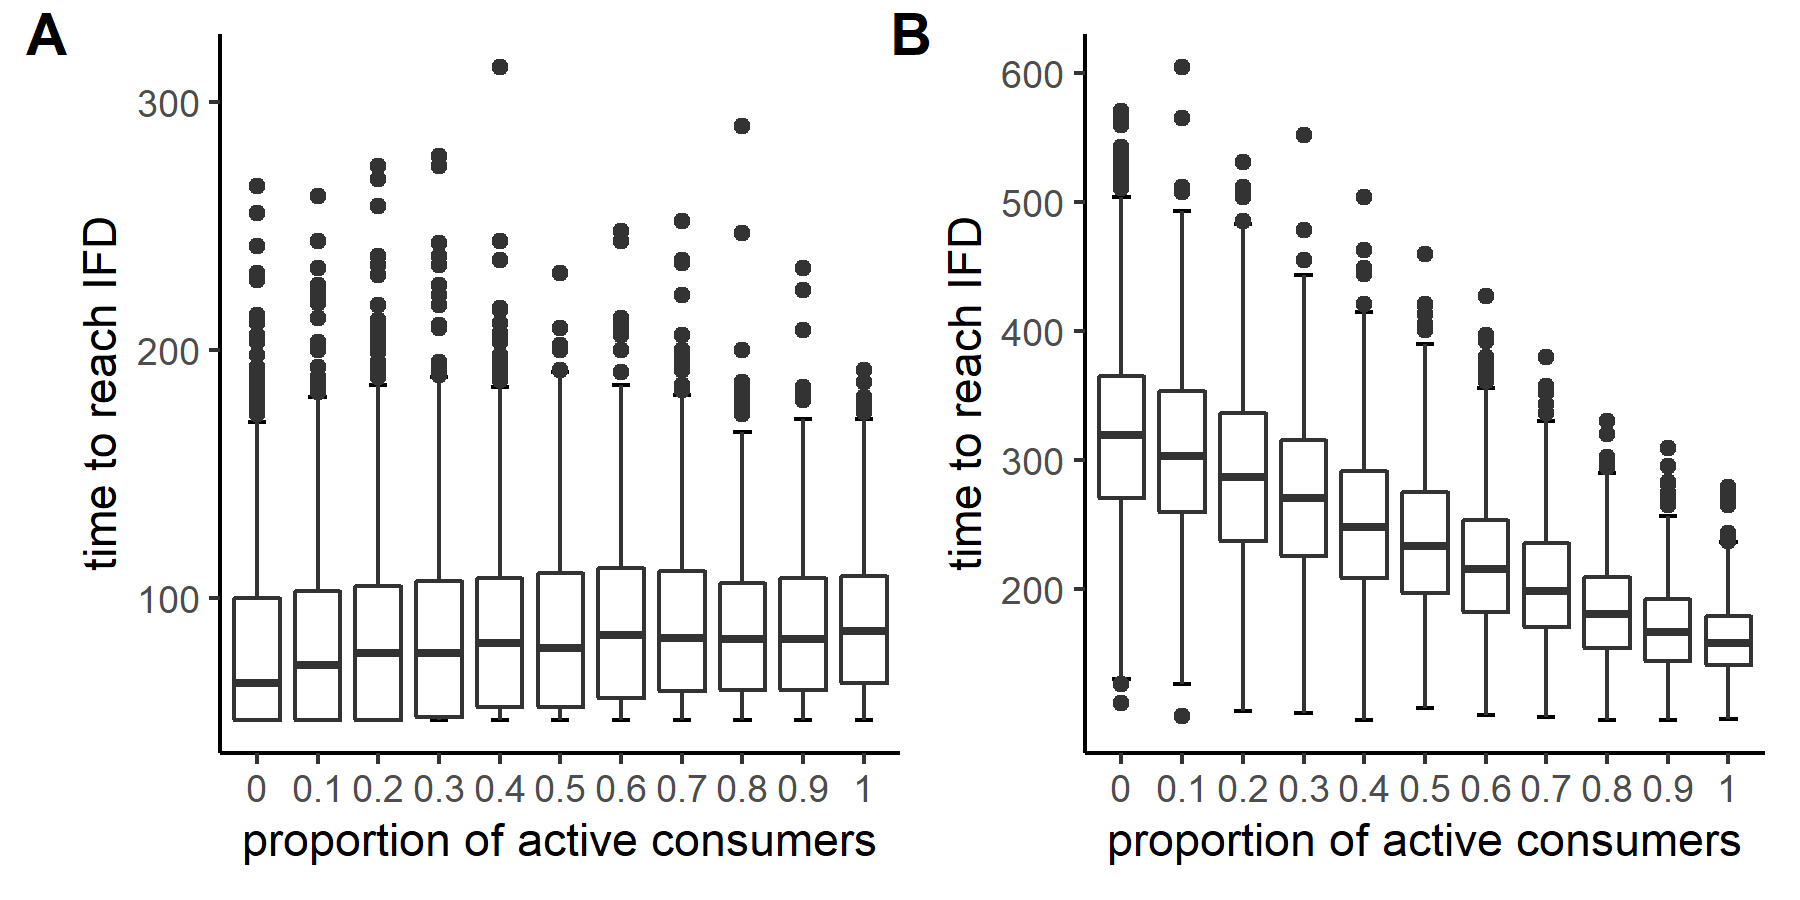
\includegraphics[width=0.9\textwidth]{figures/boxes/details1.png}
		\caption{
			Replication of DiNuzzo and Griffen's Figure S1 \textbf{(A)} using their original NetLogo code and \textbf{(B)} using a corrected version of their code. 
			Both panels show the time to reach the Ideal Free Distribution (IFD) for various proportions of ``active'' (80\% activity) and ``inactive'' (20\% activity) consumers with a type 2 functional response in 1,000 replicate simulations. 
			According to DiNuzzo and Griffen's \textit{NetLogo} code, the time- to-IFD increases with the proportion of active consumers. 
			A corrected version of the code yields the expected pattern of decreasing waiting times with increasing proportions of active consumers.
		}\label{fig_details_01}
	\end{figure}

	\begin{figure}[!h]
		\centering
		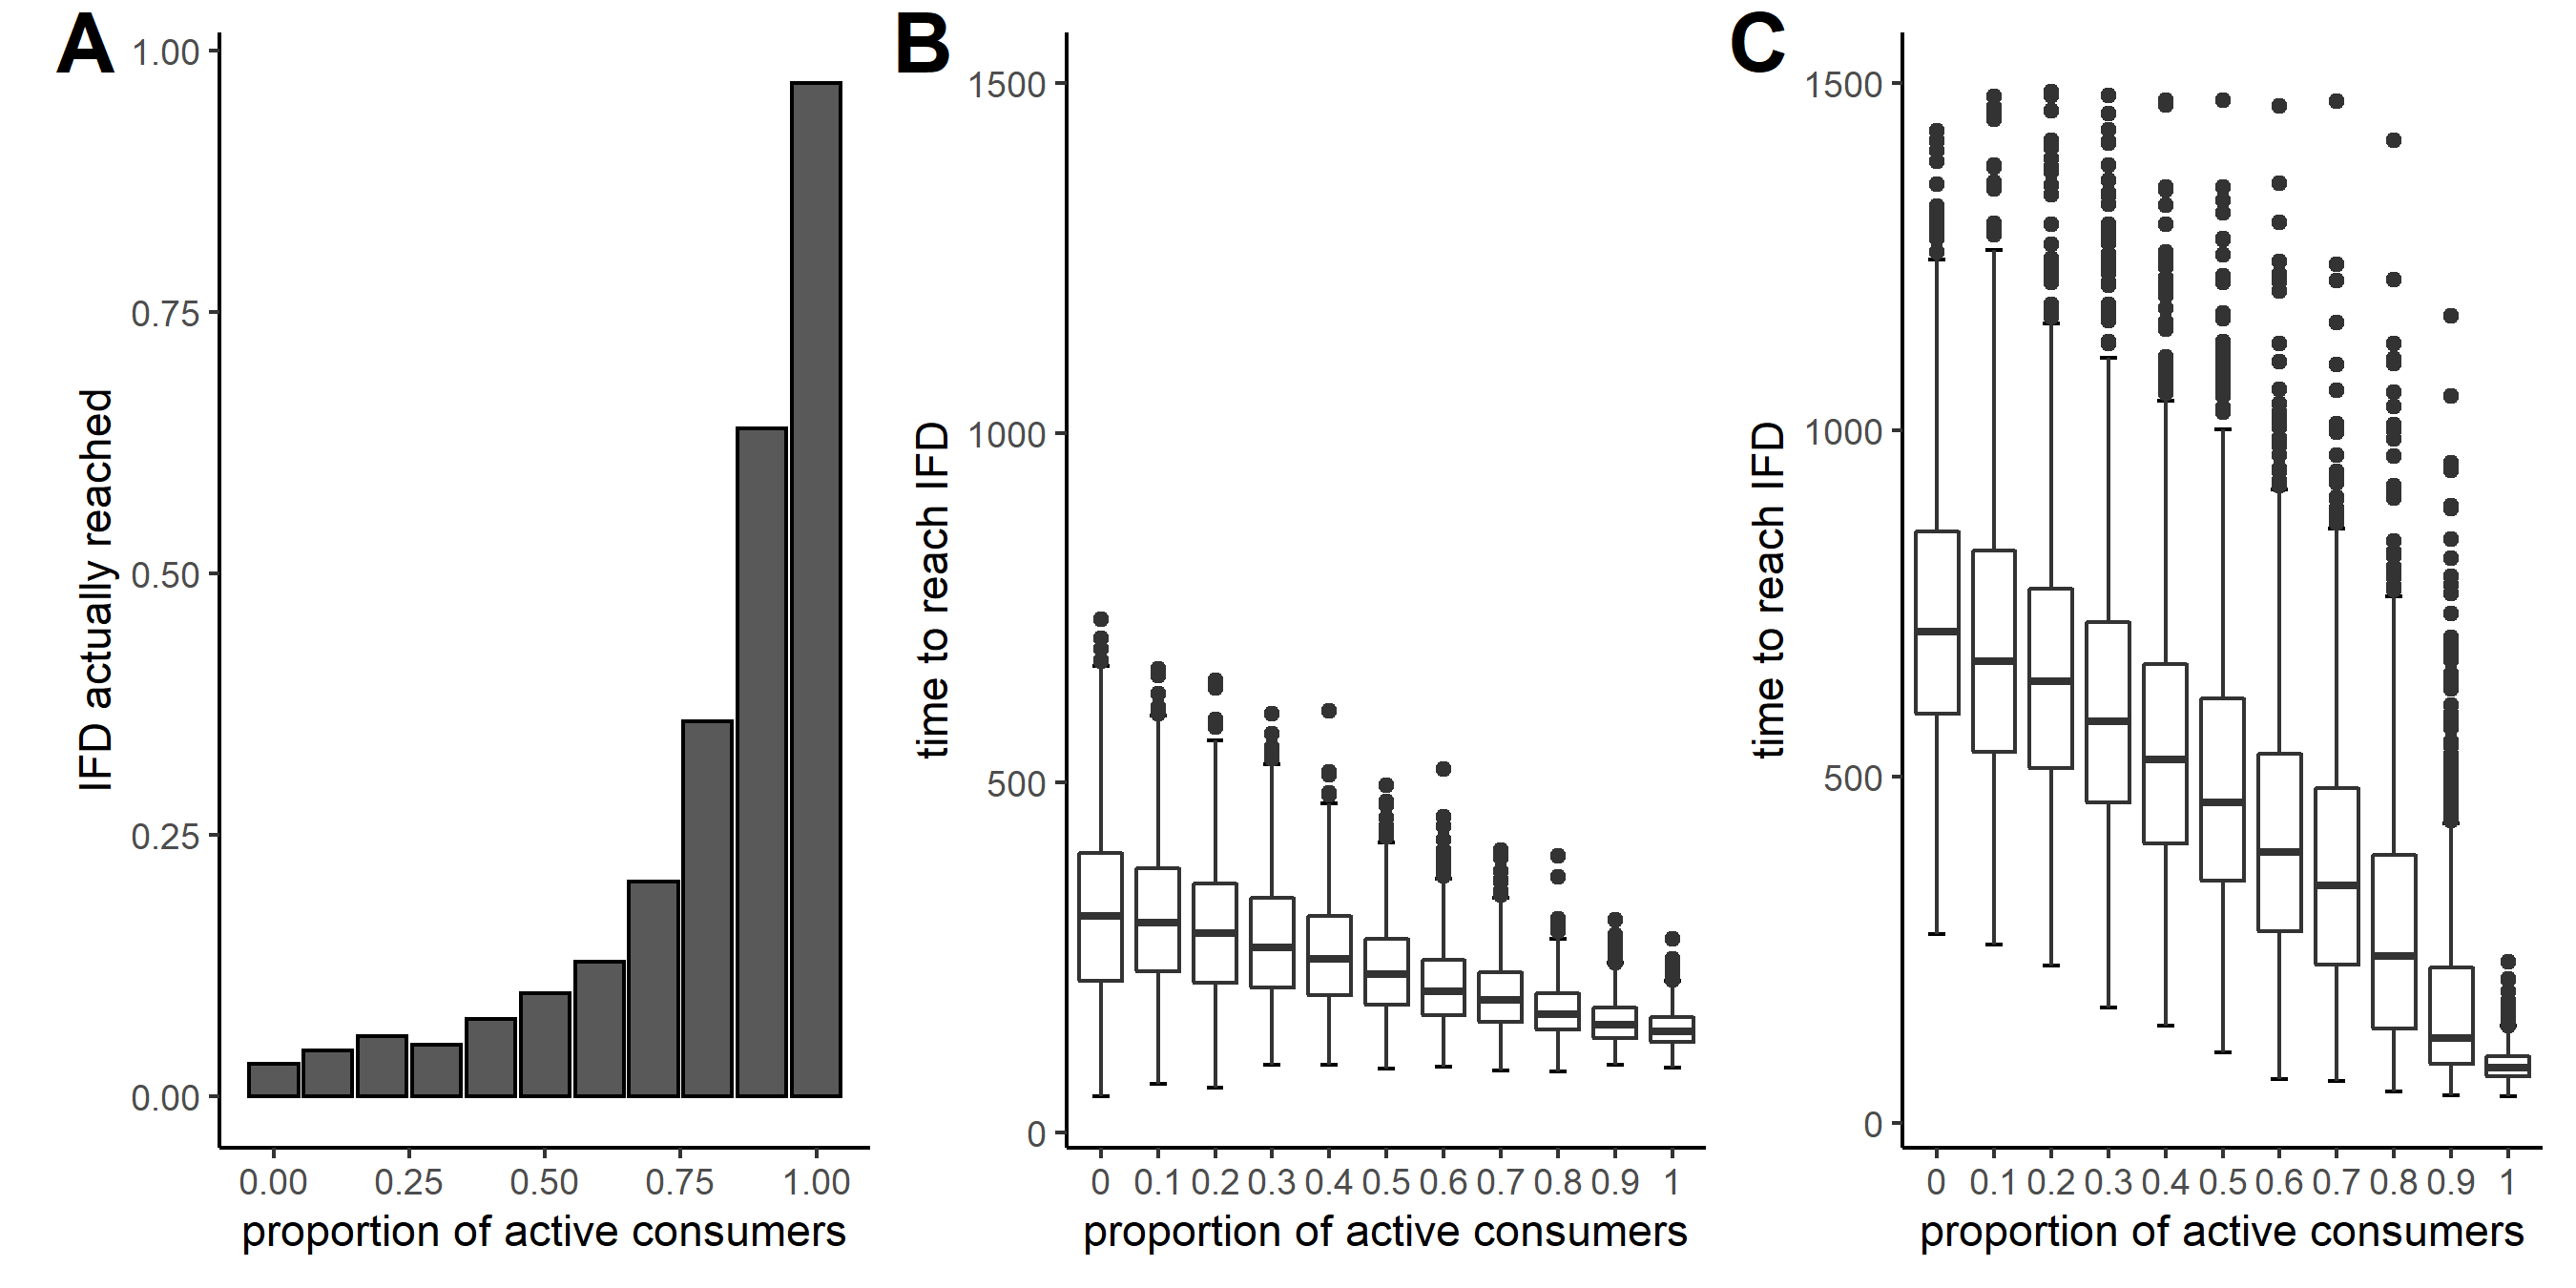
\includegraphics[width=0.9\textwidth]{figures/boxes/details2.png}
		\caption{
			Systematic bias in outcomes due to premature termination of simulations. 
			The \textit{NetLogo} code underlying the simulations in DiNuzzo and Griffen's work assumes that the IFD is reached after 50 time steps of inactivity. 
			\textbf{(A)} Proportion of simulations that have actually reached the IFD after 50 time steps in inactivity in the scenario underlying Figure 4E in \citet{dinuzzo2020}. 
			\textbf{(B)} Replication of Figure 4E, using DiNuzzo and Griffen's \textit{NetLogo} code. 
			\textbf{(C)} The same set of simulations for an improved version of the \textit{NetLogo} code, where a simulation now stops when the IFD is actually reached. 
			In all simulations, ``active'' consumers have an activity level of 90\% while ``inactive'' consumers have an activity level of 10\%.
		}\label{fig_details_02}
	\end{figure}

	\begin{figure}[!h]
		\centering
		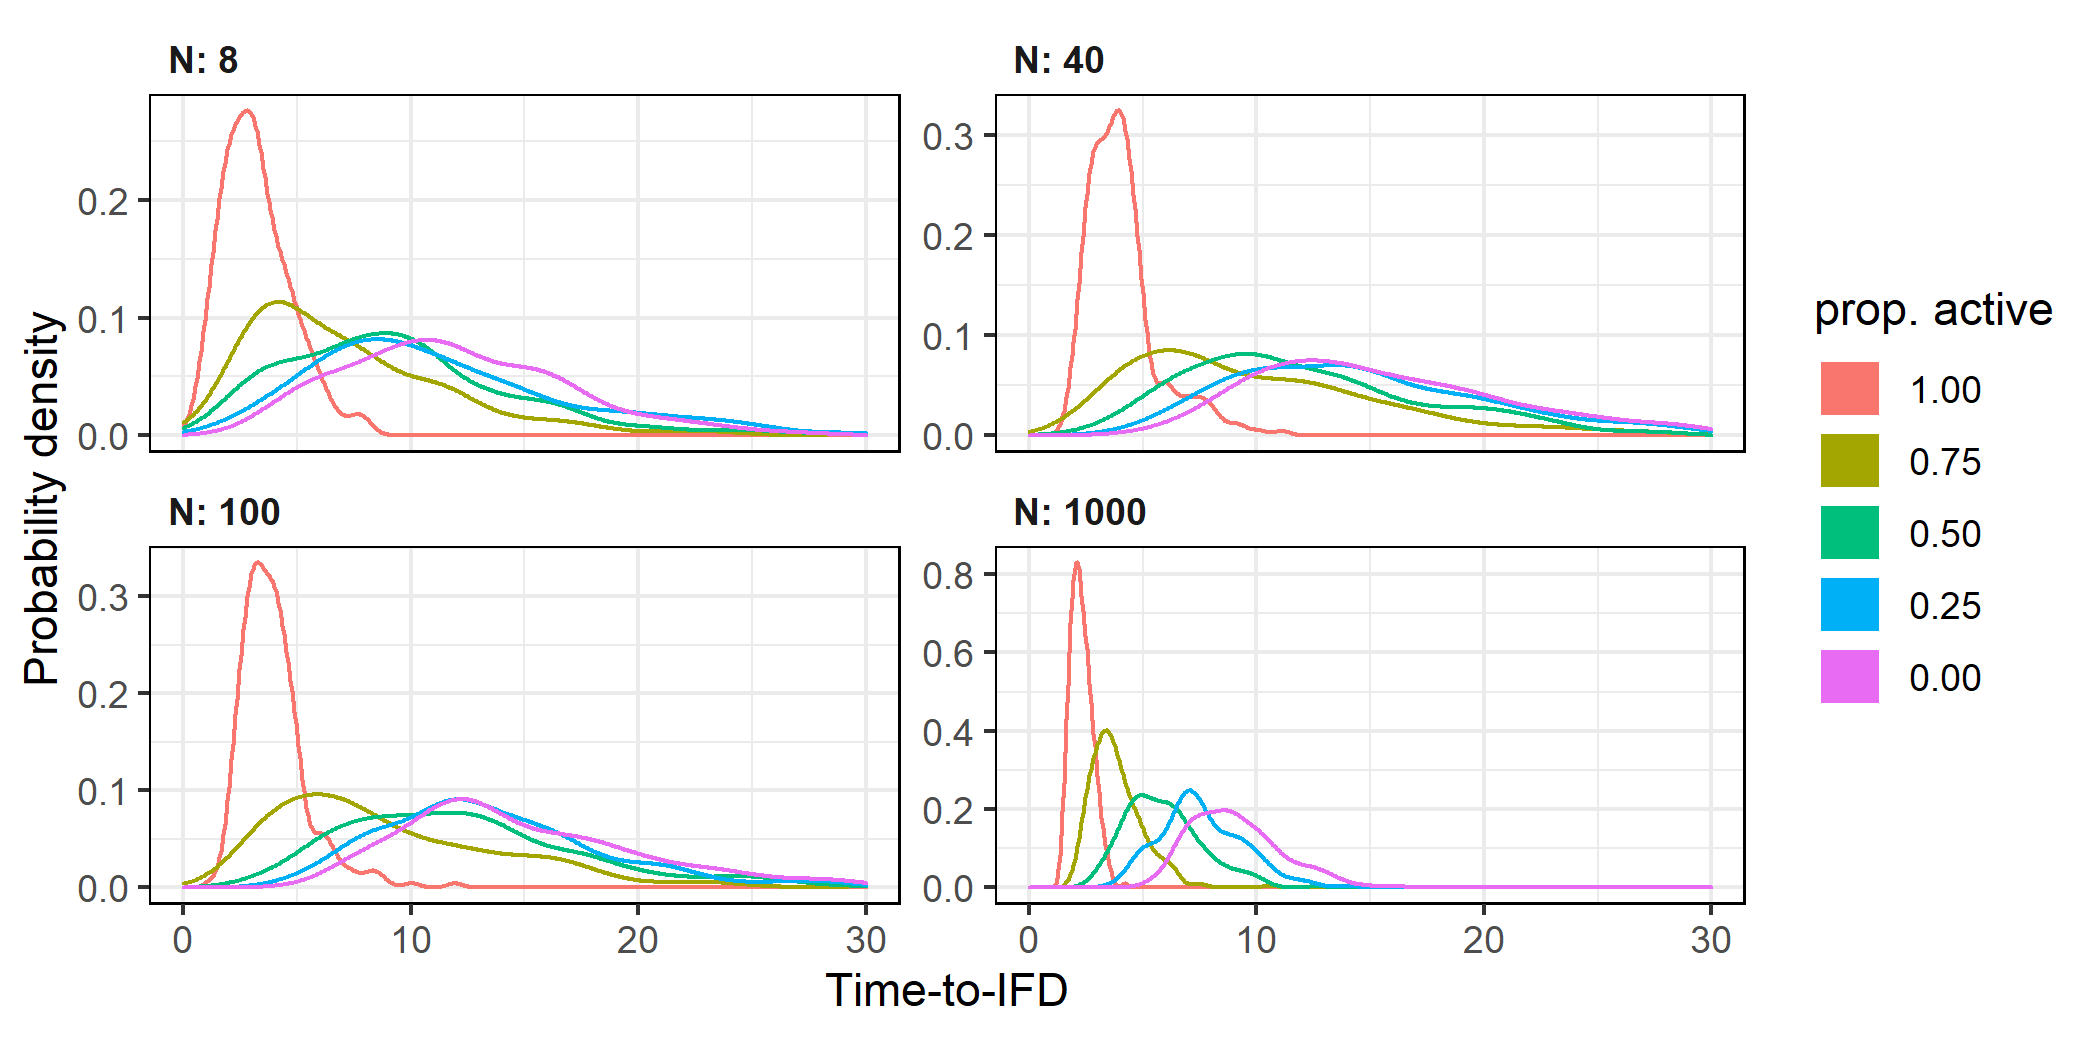
\includegraphics[width=0.9\textwidth]{figures/boxes/details3.png}
		\caption{
			Probability distributions of the time until the ideal free distribution is reached, based on 1,000 replicate simulations per setting. 
			In a system with 49 habitat patches, the panels show for four population sizes N how the time to reach IFD depends on the proportion of ``active'' (movement rate 0.8) and ``inactive'' (movement rate 0.2) individuals.
		}\label{fig_details_03}
	\end{figure}

	\subsection*{Effects of population size}
	
	DiNuzzo and Griffen investigated the effect of population size on the time to reach the IFD.
	However, the time scale of their model implementation is quite different from a `natural' time scale.
	In their simulation program, individuals make decisions sequentially, and only one individual can make a decision in each time step.
	As in a larger population more individuals have to take decisions, this automatically increases the time to reach a certain target.
	Moreover, the time to reach the IFD is inflated by the fact that active individuals are restricted in their movement because they have to ``wait'' for the inactive individuals.
	For these reasons, it is more natural to use a continuous time scale, where individuals take movement decisions independently of each other, at a rate that is proportional to their activity level.
	This can be done in a straightforward manner, by translating the discrete-time model of DiNuzzo and Griffen into an otherwise equivalent event-based model (making use of the Gillespie algorithm \footfullcite{gillespie1976} --- a description and implementation of such a model can be found in \textcite{netz2021a}\footfullcite{netz2021a}).
	Figure~\ref{fig_details_03} shows how in the event-based version of the model the time to reach the IFD depends on the population size N and the proportion of active individuals.
	For each population size, the time to reach the IFD is, as expected, positively related to the proportion of inactive individuals.
	However, the event-based version of the model does not support DiNuzzo and Griffen's conclusion that the time to reach the IFD increases with population size.
	This only occurs for very low population densities (N = 8 and N = 40 in Figure~\ref{fig_details_03}), and even in these cases the effect is small.

	At higher population sizes, the time to reach the IFD decreases with population size: as shown in Figure~\ref{fig_details_03}, the IFD is reached much faster in a population with N = 1000 individuals than in any of the smaller populations.
	This can be explained as follows.
	In case of the low population sizes considered by DiNuzzo and Griffen, the initial density of individuals is very low (typically only one individual per patch).
	In such a case, an individual can only improve its intake rate by moving to a more profitable patch.
	In case of a large population size (and a higher initial density per patch), there is an additional option: if an individual on a patch decides to leave in order to improve its intake rate elsewhere, all remaining individuals on that patch profit as their intake rate increases due to alleviated within-patch competition \footfullcite{wolf2008a}.
	This effect is not addressed by the study of DiNuzzo and Griffen, although the authors state: ``in most natural systems, there are many more consumers than patches.'' 

	\subsection*{Quantifying the approach to the IFD}
	
	DiNuzzo and Griffen conducted their study in order to investigate whether personality differences can explain ``undermatching'', the commonly observed phenomenon that high-resource patches tend to be underexploited while low-resource patches are overexploited.
	Yet, they devote only one figure (their Figure~\ref{fig_details_02}) to this phenomenon.
	In general, they quantify deviations from the IFD by measuring the time to reach the IFD.
	This measure has at least three disadvantages.
	First, ``time-to-IFD'' is determined by the last individual that moves to a patch with an optimal intake rate.
	In other words, a single individual with very low activity can have a very large effect on time-to-IFD.
	Second, ``time-to-IFD'' depends on the initial conditions; it takes longer to reach the IFD if the initial distribution of individuals over patches differs a lot from the IFD.
	Third, ``time-to-IFD'' is only a sensible measure when the IFD is actually reached.
	This, however, will only be the case in highly standardized simulation models with a fixed resource distribution.
	As stated by DiNuzzo and Griffen: ``In most systems, the IFD is a moving target owing to temporal environmental variation and directional change (i.e. habitat degradation).'' 
	In Section 1.5 of their Supplementary Information, DiNuzzo and Griffen show some simulation results for a scenario with temporally varying patch quality.
	Surprisingly, ``time-to-IFD'' is also used for this scenario (their Supplementary Figure S2), where it is difficult for us to understand how the IFD can ever be reached in case of rapid environmental change.
	How can movement cease for 50 time steps (the criterion for reaching the IFD) if the distribution of patch qualities changes completely every 10 or 20 time steps? Under such changing conditions, we would advocate using a more robust, population-level measure for deviations from the IFD, such as the variance in intake rates across patches. 
	
	\subsection*{Analysis of the mud crab system}
	
	We are puzzled by the fact that DiNuzzo and Griffen revert to a simple calculation of ratios in their analysis of the refuge use data on the mud crab \textit{Panopeus herbstii} \footfullcite{toscano2014} instead of taking advantage of their individual-based model.
	The model becomes necessary because such a simple calculation does not suffice, as it ignores the distribution of personality in the population.
	Hence, Figure 5 illustrates the influence of personality on the IFD only in the sense that no single crab is ``ideal'' in immediately leaving its refuge and moving to the patch with highest profitability, but not the implications of the distribution of activity levels in the population.
	Additionally, the data comes from a special (predation cue) treatment, not from standard conditions; and the crabs differ substantially in size (actually body size is used as a proxy for activity level) and accordingly also in their resource needs and competitive abilities. 
	
	\subsection*{Outlook}
	
	We have the impression that DiNuzzo and Griffen view ``personalities'' mainly as (maladaptive) deviations from optimal or efficient behaviour. In contrast, many studies show that personality variation is often shaped by adaptive evolution \footfullcite{wolf2012}.
	For example, Wolf and colleagues demonstrate that “inactivity” (called ``unresponsiveness'') may be viewed as an efficient strategy in achieving a high foraging success and approaching an ideal free distribution.
	An adaptive perspective on personality variation leads to novel eco-evolutionary questions regarding the interplay of individual behavioural variation and the spatial distribution of foragers.
	% The IFD is a prototype example of a model linking ecology (the spatial distribution of foragers) to evolution (optimal or evolutionarily stable movement decisions).

	Future research is needed to reconcile the IFD with the eco-evolutionary causes and consequences of personality for at least two reasons: First, the IFD model presupposes that the resource intake rate is a proxy for fitness \footfullcite{tregenza1995}.
	But how, then, can different personality types persist at stable proportions, when inactive individuals consistently achieve a lower intake rate than their more active conspecifics? 
	Second, a personality perspective may change what spatial distribution is optimal.
	In animals, differences in activity are usually associated with (adaptive) differences in energy metabolism \footfullcite{careau2008}.
	When foraging individuals differ in energetic expenditure, they should not only take maximizing the intake rate as their sole guiding principle \footfullcite{campos-candela2019}.
	In other words, individuals differing in activity should use different decision rules, and the optimal behaviour of a polymorphic population may, even at equilibrium, deviate considerably from the IFD of a monomorphic population.

	{ \begin{center} \barfont{-.-} \end{center} }

\end{interludeenv}
\endgroup

%%%%%%%%%%%%% Supplementary Information %%%%%%%%%%%%%%%

\newpage

\begingroup

\let\clearpage\relax
\let\cleardoublepage\relax
\let\cleardoublepage\relax

{\section*{Supplementary Information for Interlude~\ref{box:details}}}

The supplementary material for this interlude may be found online as Supporting Information published along with the manuscript, \textcite{netz2022}, \citetitle{netz2022}, at:
https://royalsocietypublishing.org/doi/10.1098/rspb.2021.0903.

% \newrefcontext[sorting=nyt]
% \subsection*{Literature Cited}
% \printbibliography[title=Literature~Cited~in~Interlude~\theinterludes,heading=none]
% \end{refsection}

{ \begin{center} \barfont{-.-} \end{center} }

\endgroup

\afterpage{\nopagecolor}
\pagestyle{scrheadings}


\cleardoublepage \begin{refsection}
%************************************************
\chapter{The Joint Evolution of Animal Movement and Competition Strategies}\label{ch:kleptomove}
\chaptermark{Competition and Movement}
%************************************************

{\noindent \textbf{Pratik R. Gupte}, Christoph F.G. Netz, and Franz J. Weissing}

\section*{Abstract}

{
    \small
    Competition typically takes place in a spatial context, but eco-evolutionary models rarely address the joint evolution of movement and competition strategies.
    Here we investigate a spatially explicit forager-kleptoparasite model where consumers can either forage on a heterogeneous resource landscape, or steal resource items from conspecifics (kleptoparasitism). We consider three scenarios: (1) foragers without kleptoparasites; (2) consumers specializing as foragers or as kleptoparasites; and (3) consumers that can switch between foraging and kleptoparasitism depending on local conditions.
    We model movement strategies as individual-specific combinations of preferences for environmental cues, similar to step-selection coefficients.
    Using mechanistic, individual-based simulations, we study the joint evolution of movement and competition strategies, and we investigate the implications for the distribution of consumers over this landscape.
    Movement and competition strategies evolve rapidly and consistently across scenarios, with marked differences among scenarios, leading to differences in resource exploitation patterns.
    In scenario 1, foragers evolve considerable individual variation in movement strategies, while in scenario 2, movement strategy shows a swift divergence between foragers and kleptoparasites.
    When individuals' competition strategy is conditional on local cues, movement strategies facilitate kleptoparasitism, and individual consistency in competition strategy also emerges.
    Across scenarios, the distribution of consumers differs substantially from `ideal free' predictions.
    This is related to the intrinsic difficulty of moving effectively on a depleted resource landscape with few reliable movement cues.
    Our study emphasises the advantages of a mechanistic approach when studying competition in a spatial context, and suggests how evolutionary modelling can be integrated with current work in animal movement ecology.

    \bigskip

    {\noindent \large{$\Delta$}} Under review at \textit{The American Naturalist} as Gupte et al. \citetitle{gupte2021a}.
}

% \subsection*{Data and Code}
% {
%     \small
%     Simulation model: github.com/pratikunterwegs/Kleptomove.\\ %and Zenodo: zenodo.org/record/4905476. 
%     \noindent Simulation data (DataverseNL): doi.org/10.34894/JFSC41.\\
%     \noindent Data analysis code: github.com/pratikunterwegs/klepto-move-evol.% and on Zenodo: doi.org/10.5281/zenodo.4904497.
% }

\clearpage


\newrefcontext[sorting=ynt]

\lettrine{I}{ntraspecific} competition is an important driver of population dynamics and the spatial distribution of organisms \parencite{krebs1978}, and has two main types, `exploitation' and `interference'.
In exploitation competition, individuals compete indirectly by depleting a common resource, while in interference competition, individuals compete directly by interacting with each other \parencite{birch1957,case1974,keddy2001}.
A special case of interference competition which is widespread among animal taxa is `kleptoparasitism', in which an individual steals a resource from its owner \parencite{iyengar2008}.
Since competition has an obvious spatial context, animals should account for the locations of competitors when deciding where to move \parencite{nathan2008a}.
This is expected to have downstream effects on animal distributions across spatial scales, from resource patches \parencite{fretwell1970}, to species distributions \parencite{duckworth2007,schlagel2020}.
Animal movement strategies are thus likely to be adaptive responses to landscapes of competition, with competitive strategies themselves being evolved responses to animal distributions.
Empirical studies of this joint evolution are nearly impossible at large spatio-temporal scales.
This makes models linking individual movement and competition strategies with population distributions necessary.

Contemporary individual-to-population models of animal space-use \parencite[reviewed in][]{deangelis2019} and competition, however, are only sufficient to represent very simple movement and prey-choice decisions.
% \graffito{
%     These classical foraging models correspond to real conditions as much as macro-economic models do with the real world.
%     They are likely useful only at very broad scales.
% }
For example, models including the ideal free distribution \parencite[IFD;][]{fretwell1970}, information-sharing models \parencite[][]{giraldeau1999,folmer2012}, and producer-scrounger models \parencite[][]{barnard1981,vickery1991,beauchamp2008}, often treat foraging competition in highly simplified ways.
Most IFD models consider resource depletion unimportant or negligible \parencite[continuous input models, see][]{tregenza1995, vandermeer1997}, make simplifying assumptions about interference competition, or even model an \textit{ad hoc} benefit of grouping \parencite[e.g.][]{amano2006b}.
Meanwhile, producer-scrounger models primarily examine the benefits of choosing either a producer or scrounger strategy given local conditions, such as conspecific density \parencite{vickery1991}, or the order of arrival on a patch \parencite{beauchamp2008}.
Overall, these models simplify the mechanisms by which competition decisions are made, and downplay spatial structure \parencite[see also][]{holmgren1995, garay2020, spencer2018}.

On the contrary, spatial structure is key to foraging (competition) decisions \parencite{beauchamp2008}.
How animals are assumed to integrate the costs (and potential benefits) of competition into their movement decisions has important consequences for theoretical expectations of population distributions \parencite{vandermeer1997,hamilton2002,beauchamp2008}.
In addition to short-term, ecological effects, competition also likely has evolutionary consequences for individual \textit{movement strategies}, setting up feedback loops between ecology and evolution.
Modelling competition and movement decisions jointly is thus a major challenge.
Some models take an entirely ecological view, assuming that individuals move or compete ideally, or according to fixed strategies \parencite{vickery1991,holmgren1995,tregenza1995,amano2006b}, but see \parencite{hamilton2002}.
Models that include evolutionary dynamics in movement \parencite{dejager2011,dejager2020} and foraging competition strategies \parencite{beauchamp2008,tania2012} are more plausible, but they too make arbitrary assumptions about the functional importance of environmental cues to individual decisions.

Mechanistic, individual-based models are well suited to capturing the complexities of spatial structure, animal decision-making, and evolutionary dynamics \parencite{guttal2010,kuijper2012,getz2015,getz2016,white2018,long2020,netz2021}; for conceptual underpinnings see \textcite{huston1988,mueller2011,deangelis2019}.
% \graffito{
%     I've been lucky enough to have been taught by, or to have met, many of these authors, including Vishu Guttal, Iain Couzin, Wayne Getz, Thomas M\"uller, and Don DeAngelis.
% }
% \graffito{
%     Reading Lauren White's implementation of movement decisions as resource selection functions \parencite{white2018} was instrumental in how I thought about my work.
%     Her model also inspired Chapter~\ref{ch:pathomove}.
% }
Individual-based models can incorporate the often significant variation in movement and competition preferences found in populations, allowing individuals to make different decisions given similar cues \parencite[][]{laskowski2013}.
Individual-based models also force researchers to be explicit about their modelling assumptions, such as \textit{how exactly} competition affects fitness.
Similarly, rather than taking a purely ecological approach and assuming individual differences \parencite[e.g. in movement rules:][]{white2018}, allowing movement strategies to evolve in a competitive landscape can reveal whether individual variation emerges in plausible ecological scenarios \parencite[as in][]{getz2015}.
This allows the functional importance of environmental cues for movement \parencite[see e.g.][]{scherer2020} and competition decisions in evolutionary models to be joint outcomes of selection, and lets different competition strategies to be associated with different movement strategies \parencite[][]{getz2015}.

Here, we present a spatially-explicit, mechanistic, individual-based model of intraspecific foraging competition, where movement and competition strategies jointly evolve on a resource landscape with discrete, depletable food items that need to be processed (`handled') before consumption.
% \graffito{
%     The Kleptomove model's source code is adapted from an earlier predator-prey model
%     \parencite{netz2021}.
% }
In our model, foragers make movement decisions using inherited, evolvable preferences for local ecological cues, such as resource and competitor densities; the combination of preferences for each cue forms individuals' movement strategy \parencite[similar to relative step-selection:][]{fortin2005, avgar2016}.
Lifetime resource consumption is our proxy for fitness; more successful individuals produce more offspring, transmitting their movement and foraging strategies to future generations (with small mutations).
We consider three scenarios: in the first scenario, we examine only exploitation competition.
In the second scenario, we introduce kleptoparasitic interference as an inherited strategy, fixed through an individual's life.
In the third scenario, we model kleptoparasitism as a behavioural strategy conditioned on local environmental and social cues; the mechanism underlying this foraging choice is also inherited.

Our model allows us to examine the evolution of individual movement strategies, population-level resource intake, and the spatial structure of the resource landscape.
The model enables us to take ecological snapshots of consumer-resource dynamics (animal distributions, resource depletion, and competition) proceeding at evolutionary time-scales.
Studying these snapshots allows us to check whether, when, and to what extent the spatial distribution of competitors resulting from the co-evolution of competition and movement strategies corresponds to standard IFD predictions.
We investigate \textit{(1)} which movement strategies evolve in our three competition scenarios, \textit{(2)} whether movement strategies differ within and between competition strategies in our scenarios, and \textit{(3)} whether the emergent spatial distributions of consumers corresponds to `ideal free' expectations.

\section*{The Model}

Individual-based models have to explicitly specify numerous assumptions (e.g. spatial structure, individual interactions, event timescales), but this helps expose assumptions that are often hidden below the surface in analytical models. 
We kept our model assumptions as simple and generic as possible, striving for general, conceptual insights.
To keep the model realistic, we based it on the foraging behavior of shorebirds such as oystercatchers (\textit{Haematopus} spp.), which are extensively studied in the context of foraging competition, both empirically \parencite[e.g.][]{vahl2005, vahl2005a,vahl2007a, rutten2010, rutten2010a}, and using individual-based models \parencite[reviewed in][]{stillman2010}.

% \graffito{
%     We initially tried 100 timesteps, but settled on 400 as this allowed enough time for individuals' intake to be a function of their movement strategy, rather than their good fortune in being initialised in a productive part of the landscape.
% }
Our environment is a fine grid of cells, and each grid cell can hold multiple individuals.
Resources are discrete, as is our conception of time within and between generations. 
Our population, with a fixed number of individuals (N = 10,000), moves on a landscape of 512\textsuperscript{2} grid cells (approx. 1 individual per 26 cells), with wrapped boundaries (i.e., a torus); individuals passing beyond the bounds at one end re-appear on the opposite side.
The model has two time scales, first, an ecological time scale of $T$ timesteps comprising one generation (default $T$ = 400), during which individuals move, make foraging decisions, and handle prey-items they find or steal.
Individuals are immobile while handling food items, creating the conditions for kleptoparasitism \parencite{brockmann1979,ruxton1992}.
At the end of each generation, individuals reproduce, transmitting their movement and foraging strategies to their offspring, whose number is proportional to individual intake at the ecological time scale.
Our model has 1,000 generations, and this comprises the evolutionary timescale.

\subsection*{Resource Landscape}

\paragraph{Prey Abundance}

% \graffito{
%     Early versions of this model had one giant resource peak; this was dropped as it was relatively easy for individuals to find their way to productive areas.
% }
We considered our discrete resources, called `prey-items' to represent mussels, a common prey of many shorebirds, whose abundances are largely driven by external gradients.
We assigned each cell a constant probability of generating a new prey-item per timestep, which we refer to as the cell-specific growth rate $r$.
We modelled clustering in landscape productivity by having the distribution of $r$ across the grid take the form of 1,024 resource peaks, placed at regular distances of 16 grid cells from the peaks around them; $r$ declines from the centre of each peak (called $r_{max}$) to its periphery (see Fig.~\ref{klepto_fig_01}A).
Thus the central cell generates prey-items five times more frequently than peripheral cell: at $r_{max}$ = 0.01, central cells generate one item per 100 timesteps (four items/generation), while the peripheral cells generate one item only every 500 timesteps ($<$ one item/generation).
All landscape cells have a uniform carrying capacity $K$ of 5 prey-items.
While a cell is at carrying capacity its $r$ is 0.
Cells are initialised with prey-items proportional to their $r$ (see e.g. Fig.~\ref{klepto_fig_01}A).

\paragraph{Prey Acquisition by Foragers}

Foragers perceive a cue indicating the number of prey-items $P$ in a cell, but fail to detect each item with a probability $q$, and are thus successful in finding a prey-item with a probability $1 - q^P$.
Individuals on a cell forage in a randomised sequence, and the probability of finding a prey-item ($1 - q^P$) is updated as individuals find prey, reducing $P$.
Foragers that find a prey-item must handle it for a fixed handling time $T_H$ (default = 5 timesteps), before consuming it \parencite[][]{ruxton1992}.
Natural examples include the time required for an oystercatcher to break through a mussel shell, or a raptor to subdue prey; overall, the handling action is obvious, and the prey is not fully under the control of the finder \parencite{brockmann1979}.
Foragers that do not find a prey-item are considered idle in that timestep, and are counted as `non-handlers'.
Similarly, handlers that finish processing their prey in timestep $t$ can only forage again in timestep $t+1$, i.e., they are idle in the timestep $t$.

\subsection*{Movement Strategies}

All individuals move simultaneously at the end of each timestep $t$, and then implement their foraging or kleptoparasitic behaviour to acquire prey.
However, handlers do not make any movements until they have fully handled and consumed their prey.
We model movement as comprised of small, discrete steps between adjacent cells.
Across scenarios, individuals make movement decisions using evolved cue preferences.
Individuals select a destination cell, after assessing potential destinations based on available cues, similar to approaches used previously \parencite{getz2015,getz2016,white2018,scherer2020,netz2021}.

% \graffito{
%     Our individuals can use much more complex functions, encoded by neural networks, an idea that has been explored, but not widely used, in movement ecology \parencite{mueller2011}.
% }
To move, individuals scan the nine cells of their Moore neighbourhood for three environmental cues, \textit{(1)} an indication of the number of discrete prey-items $P$, \textit{(2)} the number of individuals handling prey $H$ (`handlers'), and \textit{(3)} the number of individuals not handling prey $N$ (`non-handlers').
Individuals rank the potential destinations (including their current cell) by their suitability $S$, where $S = s_PP + s_HH + s_NN$, and move to the most suitable cell in timestep $t+1$.
The individual preferences for each cue, $s_P$, $s_H$, and $s_N$, have numeric values, are considered to be evolvable traits that can be transmitted between generations, and undergo independent mutation.
Since individuals are constrained to perceiving and moving short distances, they may not always sense their best long-term move.

It is the combination of cue preferences, and especially their value relative to each other, that determines individual movement decisions \parencite[similar to relative selection coefficients,][]{fortin2005,avgar2016,white2018}. 
For example, an extreme value of $s_P$ relative to the other preferences would mean that an individual's movement decisions are guided primarily by differences in the local density of prey-items.
We call an individual's combination of inherited preferences its \textit{movement strategy} (see e.g. Fig.~\ref{klepto_fig_01}E).

\subsection*{Competition Strategies}

\paragraph{Scenario 1: Exploitative Competition}

In scenario 1, we simulate only exploitative competition; individuals (henceforth called `foragers') move about on the landscape and probabilistically find, handle, and consume prey-items.
Foragers can be either in a `searching' or a `handling' state \parencite{holmgren1995}.

\paragraph{Scenario 2: Foraging or Kleptoparasitism as Fixed Strategies}

% \graffito{
%     The Kleptomove simulation can be modified to change the probability of kleptoparasite success.
% }
In scenario 2, the competition strategy is genetically determined and transmitted from parents to offspring: exploitative competition (by foragers), or kleptoparasitic interference (by kleptoparasites).
Kleptoparasites cannot extract prey-items directly from the landscape, and only steal from handlers \parencite[see][]{holmgren1995}.
Kleptoparasites are always successful in stealing from handlers, and such successful surprise attacks are commonly observed among birds \parencite{brockmann1979}.
When multiple kleptoparasites target the same handler, only one (randomly selected) is considered successful --- thus kleptoparasites compete exploitatively among themselves.
Kleptoparasites displace the handler that they robbed of prey up to 5 cells away from their location.
Having acquired prey, kleptoparasites become handlers, but need only handle prey for $T_H - t_h$ timesteps, where $t_h$ is the time that the prey has already been handled by its previous owner.
Once a kleptoparasite becomes a handler, it can also be targeted by other kleptoparasites.
Unsuccessful kleptoparasites are considered idle, and are counted as non-handlers.
Movement strategies evolve independently of the competition strategy, as in scenario 1; however, the optimal movement strategy for foragers need not be the same as that for kleptoparasites.

\paragraph{Scenario 3: Conditional Interference Competition}

% \graffito{
%     Similar to movement decisions, competition decisions can also be encoded by a neural network.
% }
In scenario 3, each individual can either act as a forager, or as a kleptoparasite, depending on its assessment of local conditions.
Similar to how movement decisions are made based on local cues, individuals process cell-specific environmental cues in timestep $t$ to determine their competition strategy in the next timestep as
% \begin{linenomath*}
\begin{equation}
    \text{strategy} = 
\begin{cases}
    \text{forager},& \text{if } w_PP + w_HH + w_NN \geq w_0\\
    \text{kleptoparasite},              & \text{otherwise}
\end{cases}
\end{equation}  
% \end{linenomath*}
where the cue preferences $w_P$, $w_H$ and $w_N$, and the threshold value $w_0$, are numeric values, and heritable between generations (with small, rare, independent mutations).
The combination of the cue preferences for competition decisions forms each individual's \textit{competition strategy}.
Individuals' competition strategies may lead to specialisation as foragers or kleptoparasites (as in scenario 2), or to plastic behaviour conditioned on local cues.
The competition dynamics are the same as in scenario 2.

\subsection*{Reproduction and Inheritance}

Our model considers a population of fixed size (10,000 individuals) with discrete, non-overlapping generations. 
For simplicity, we assume that individuals are haploid and reproduction is asexual. 
In scenarios 1 and 2, individuals only inherit and transmit their cue preferences ($s_P$, $s_H$, $s_N$) which determine movement decisions.
In scenario 3, individuals also inherit cue preferences for competition decisions ($w_P$, $w_H$, $w_N$, $w_0$), and transmit them to offspring.
The movement and competition cue preferences all mutate independently in scenario 3.
% \graffito{
%     The implicit assumption here is fecundity effects, rather than mortality effects. This is consistent with many shorebirds, which often fail to breed in bad years, but have very high adult survival.
% }
Each individual's number of offspring is proportional to the individual's total lifetime intake of resources; hence, resource intake is used as a proxy for fitness. 
A weighted lottery (with weights proportional to lifetime resource intake) selects a parent for each offspring in the subsequent generation \parencite[see e.g.][]{tania2012,netz2021}.
Across scenarios, the cue preferences for movement decisions are subject to rare, independent mutations ($\mu$ = 0.001).
The mutational step size (either positive or negative) is drawn from a Cauchy distribution with a scale of 0.01 centred on zero, allowing for a small number of very large mutations while most mutations are small.
In scenario 2, foragers may infrequently mutate into a kleptoparasite (or \textit{vice versa}; $\mu$ = 0.001).
In scenario 3, the competition cue preferences also mutate as described above.
Each offspring is initialised at random locations on the landscape, leading individuals to experience conditions potentially different from those of their parent.
We chose this option because it allows us to focus on adaptive movement strategies, whereas limited dispersal confounds movement and local adaptation.

\subsection*{Simulation Output and Analysis}

% \graffito{
%     The simulation output, in a Windows-specific compressed format, required a number of specialised functions to extract useful information.
% }
We ran all three scenarios at a default $r_{max}$ of 0.01, which we present in the \textsc{Results}, and also across a range of $r_{max}$ values between 0.001 and 0.05 (see Fig.~\ref{klepto_fig_06} and Supplementary Material Figs. 7 -- 9).
We initialised the cue preferences with values drawn from a Cauchy distribution with a scale of 0.01 centred on zero; this allows a very small amount of variation in the population (see e.g. Fig.~\ref{klepto_fig_01}E), and is equivalent to a single generation of mutation from all preferences initialised at zero (see \textsc{Reproduction and Inheritance} above).
Normalising each individual's cue preferences by the sum of the absolute values of all preferences $s_I = s_I / (|s_P| + |s_H| + |s_N|)$, for $s_I \in s_P, s_H, s_N$, makes it possible to visualise individuals on a three-dimensional trait space of relative preferences bounded by (-1.0: \textit{strongly avoid}, +1.0: \textit{strongly prefer}).
With remarkably consistent outcomes across replicates in each scenario, and as each simulation run produced massive datasets, we show the outcomes of three replicates here.
More data can be generated and analysed using the code linked below.

\paragraph{Population Activities and Intake}

Across scenarios, in each generation, we counted the number of times foragers were searching for prey, kleptoparasites were searching for handlers, and the number of timesteps that individuals of either strategy were handling a prey-item.
We refer to the ratio of these values as the population's `activity budget'.
We examined how the population activity budget developed over evolutionary time, and whether a stable equilibrium was reached.
Furthermore, we counted the population's mean per-capita intake per generation as a measure of population productivity.

\paragraph{Visualising Movement Strategies}

To understand the evolution of individual movement and competition strategies, we exported the cue preferences of each individual in every generation of the simulation.
We scaled each cue preference by the sum of the absolute values of the preferences, allowing us to plot individuals in a standardised three-dimensional trait space of relative cue preferences (with colour as an axis on a two-dimensional plot).
Individuals' position in this space allowed us to easily visualise and compare variation in movement strategies within and between competition strategies and across scenarios.

\paragraph{Visualising Scenario 3 Competition Strategies}

Scenario 3 competition strategies are determined by four values (3 preferences and threshold value), and competition decisions are outcomes of the interactions of these preferences with individuals' movement decisions and ecological conditions.
This makes strategies \textit{per se} difficult to visualise.
We first scaled the competition cue preferences and the threshold value as we did the movement cue preferences.
To illustrate variation in the competition strategies evolved, we presented each individual in representative generations (G = 10, 30, 100, 300, 950) with combinations of two key cues, handler and prey density (each 0 -- 5; 36 combinations overall).
We summarised the proportion of individuals that would attempt to steal at each combination of cue values (see Eqn. 1; Fig.~\ref{klepto_fig_04}F).

\paragraph{Ecological Snapshots of Consumer-Resource Distributions}

We exported snapshots of the entire simulation landscape at the mid-point of each generation ($t$ = 200).
Each snapshot contained data on \textit{(1)} the number of prey-items, \textit{(2)} the number of handling individuals, and the number of individuals using either a \textit{(3)} searching forager strategy or \textit{(4)} kleptoparasitic strategy, on each cell.
We used a subset of the total landscape (60\textsuperscript{2} of 512\textsuperscript{2} cells) for further analyses to speed up computation.
We determined the availability of direct resource cues for movement in each cell by calculating the cell-specific item gradient for each landscape snapshot, as the difference in prey counts between each cell and its neighbouring cells.
For each generation, we calculated the proportion of cells from which it was possible to sense differences in prey-items, i.e., a neighbouring cell with either more or fewer items.

\paragraph{Testing the Input Matching Rule}

A basic prediction of the IFD and the related matching rule is that the number of individuals on occupied patches should be proportional to patch productivity \parencite{fretwell1970,parker1978,houston2008}.
Patch productivity is challenging to measure in real world systems, but is among our model's building blocks, and we examined the correlation between the number of individuals (excluding handlers) and the cell-specific productivity $r$, expecting large positive values.

\section*{Results}

\subsection*{Scenario 1: No Kleptoparasitism}

In scenario 1, foragers deplete prey-items faster than they are replenished, drastically reducing the overall number of prey within 50 generations (Fig.~\ref{klepto_fig_01}A).
The population activity budget is split between searching and handling (Fig.~\ref{klepto_fig_01}B); while handling and the mean per-capita intake are both initially low, they peak within ten generations (Fig.~\ref{klepto_fig_01}C), as individuals easily acquire prey-items from the fully stocked landscape in the first few generations.
With dwindling prey-items, fewer searching foragers find prey, and handling as a share of the activity budget declines to a stable $\sim$ 45\% within 50 generations, and mean per-capita intake also stabilises (Fig.~\ref{klepto_fig_01}C).
Across generations, the correlation between the number of foragers and cell productivity is only slightly positive (Fig.~\ref{klepto_fig_01}D).
This is in contrast with the perfect correspondence between resource input rate and forager density (the `input matching rule'), which is a defining property of the IFD \parencite{parker1978, houston2008}.
Contrary to standard IFD assumptions, foragers cannot directly sense the local cell productivity $r$; instead they can only use the (small) number of prey-items available in a cell as a cue for local productivity.
A wide range of movement strategies co-exist on the landscape (see all generations in Supplementary Material Fig.~2, 6).
Some individuals mostly move up gradients of prey-items (Fig.~\ref{klepto_fig_01}E; $s_P$ $\approx$ 1.0), some move primarily towards successful foragers (handlers), while others move away from unsuccessful foragers which are potential competitors (more red $s_N$).

\begin{figure}[t!]
    \centering
    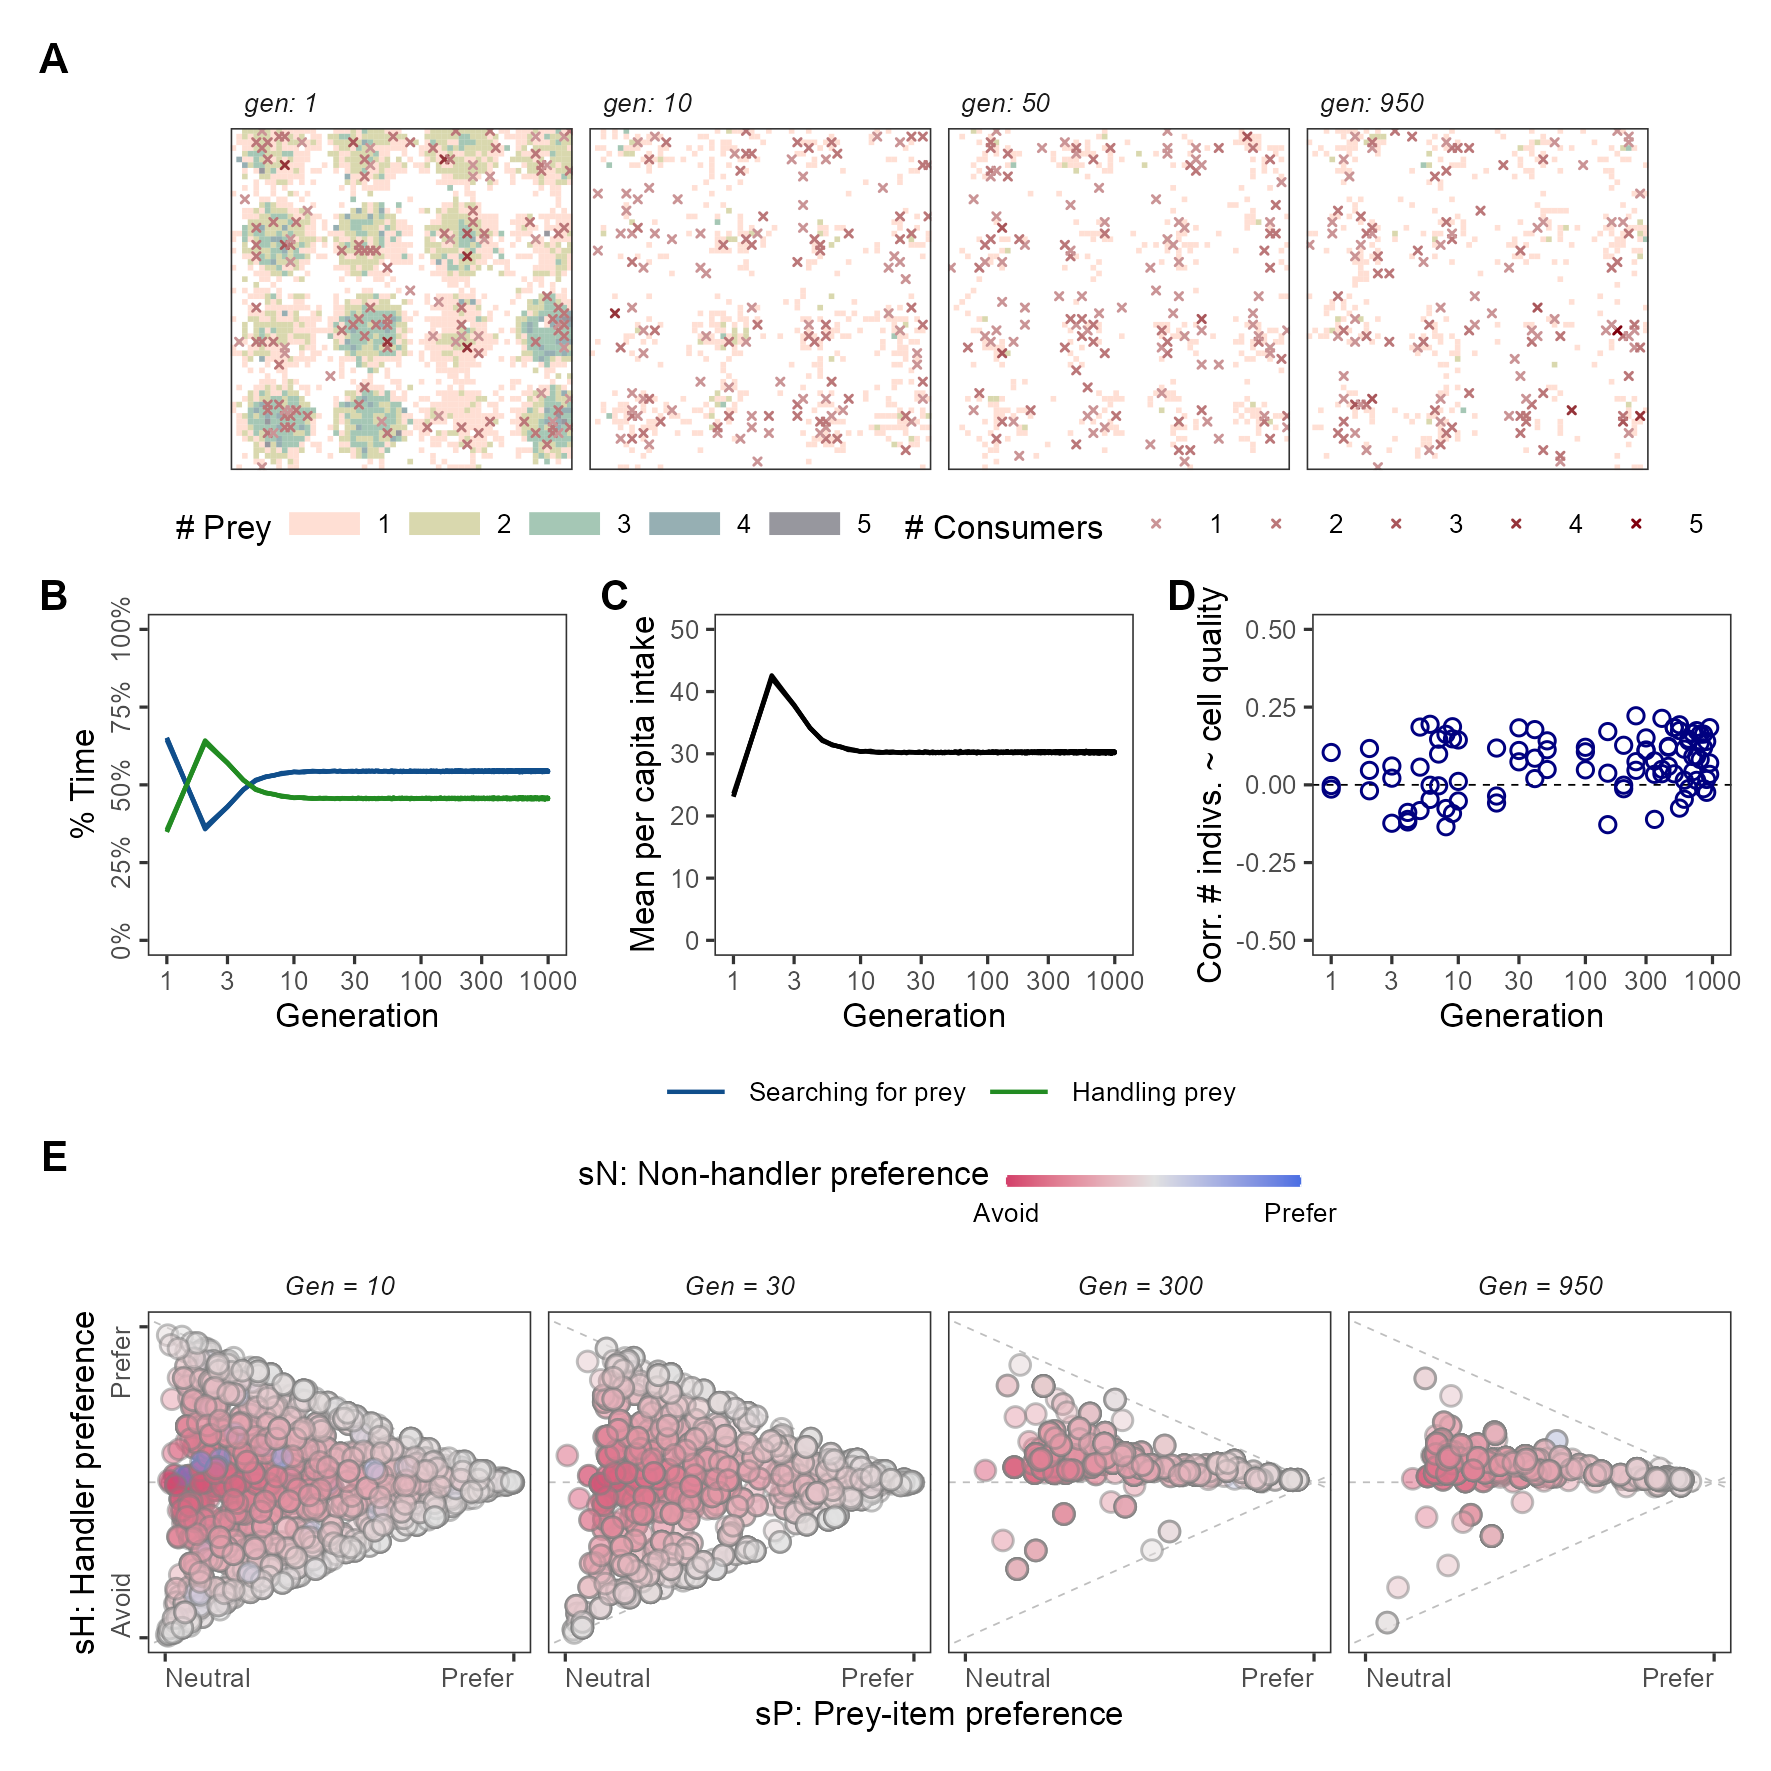
\includegraphics[width=0.7\textwidth]{figures/kleptomove/fig_01.png}
    \caption{
        \textbf{Eco-evolutionary implications of pure exploitation competition in scenario 1.}
        \textbf{(A)} A population comprised solely of foragers seeking prey on a resource landscape swiftly depletes initially abundant prey-items within 10 generations (of 1,000 simulated).
        Foragers maintain this prey-item scarcity throughout the remaining generations of the simulation, despite regular resource regeneration (see G = 950).
        \textbf{(B)} Within 20 generations of evolution, the population reaches an equilibrium in the relative proportion of time spent on searching for prey and handling prey, and in \textbf{(C)} mean per-capita intake.
        \textbf{(D)} The number of foragers per cell is only weakly correlated with cell productivity $r$, contrary to the input matching rule of Ideal Free Distribution theory.
        \textbf{(E)} A wide range of movement strategies co-exist on the landscape over hundreds of generations.
        Individuals may focus on moving up gradients of prey-items (sP $\approx$ 1.0: \textit{prefer}), moving towards successful foragers (handlers), or moving away from unsuccessful foragers which are potential competitors (sN $\approx$ red).
        Panels \textbf{A, E} show a single replicate, panels \textbf{B, C, D} and \textbf{D} show three replicate simulations with log-scaled X-axes (lines overlap almost perfectly); all panels are for $r_{max}$ = 0.01; panel \textbf{E} shows 2,500 individuals.
    }
    \label{klepto_fig_01}
\end{figure}

\subsection*{Scenario 2: Co-existence of Foragers and Kleptoparasites}

In scenario 2, with fixed foraging and kleptoparasitism allowed, the spatial distribution of prey-items at equilibrium is very different from scenario 1.
Consumers graze down resource peaks until few prey-items remain on the landscape; however, within 50 generations the resource landscape recovers with prey abundances higher than in the earliest generations (Fig.~\ref{klepto_fig_02}A).
This is because of the emergence of kleptoparasites (Fig.~\ref{klepto_fig_02}B): in early generations, kleptoparasites are rare, and the activity budget, the mean per-capita intake, and the distribution of consumers over the landscape, are similar to scenario 1.
As resources are depleted and kleptoparasite-handler encounters become more common than forager-prey encounters, kleptoparasitism becomes the majority strategy (a stable $\sim$70\% of the population; see Fig.~\ref{klepto_fig_02}B), and searching for handlers to rob becomes the commonest activity.
However, the high frequency of this activity and the low frequency of handling, indicate that few kleptoparasites are successful at robbing handlers.

With few foragers, few prey-items are extracted from the landscape, which recovers beyond its initial prey abundance within 50 generations (Fig.~\ref{klepto_fig_02}A).
As fewer prey-items are extracted overall, mean per-capita intake also declines from an initial peak (Fig.~\ref{klepto_fig_02}C).
Despite the strong spatial structure of the resource landscape within 50 generations, the correlation between consumers (of either strategy) and cell productivity remains weak or zero across generations (Fig.~\ref{klepto_fig_02}D).
This may be partially explained by the ecology of kleptoparasitism: foragers are regularly displaced by kleptoparasites, and kleptoparasites must themselves move to find handlers.

There is a sharp evolutionary divergence of movement strategies between foragers and kleptoparasites.
While both foragers and kleptoparasites evolve to prefer prey and avoid non-handlers, their response to handlers is very different (Fig.~\ref{klepto_fig_03}; see also Supplementary Material Fig.~3, 5).
Kleptoparasites very rapidly evolve a strong preference for moving towards handlers, which are their primary resource (Fig.~\ref{klepto_fig_03}).
In the absence of kleptoparasites, foragers would also evolve a similar preference (Fig.~\ref{klepto_fig_01}E), but, with kleptoparasites common in the population, foragers converge upon a handler-avoiding strategy (Fig.~\ref{klepto_fig_03}).
This completes the explanation for why consumers do not match landscape productivity: foragers evolve strategies to avoid high productivity areas (which are more likely to have many handlers), while kleptoparasites evolve strategies to find handlers (which need not be on high productivity cells).

\begin{figure}[t!]
    \centering
    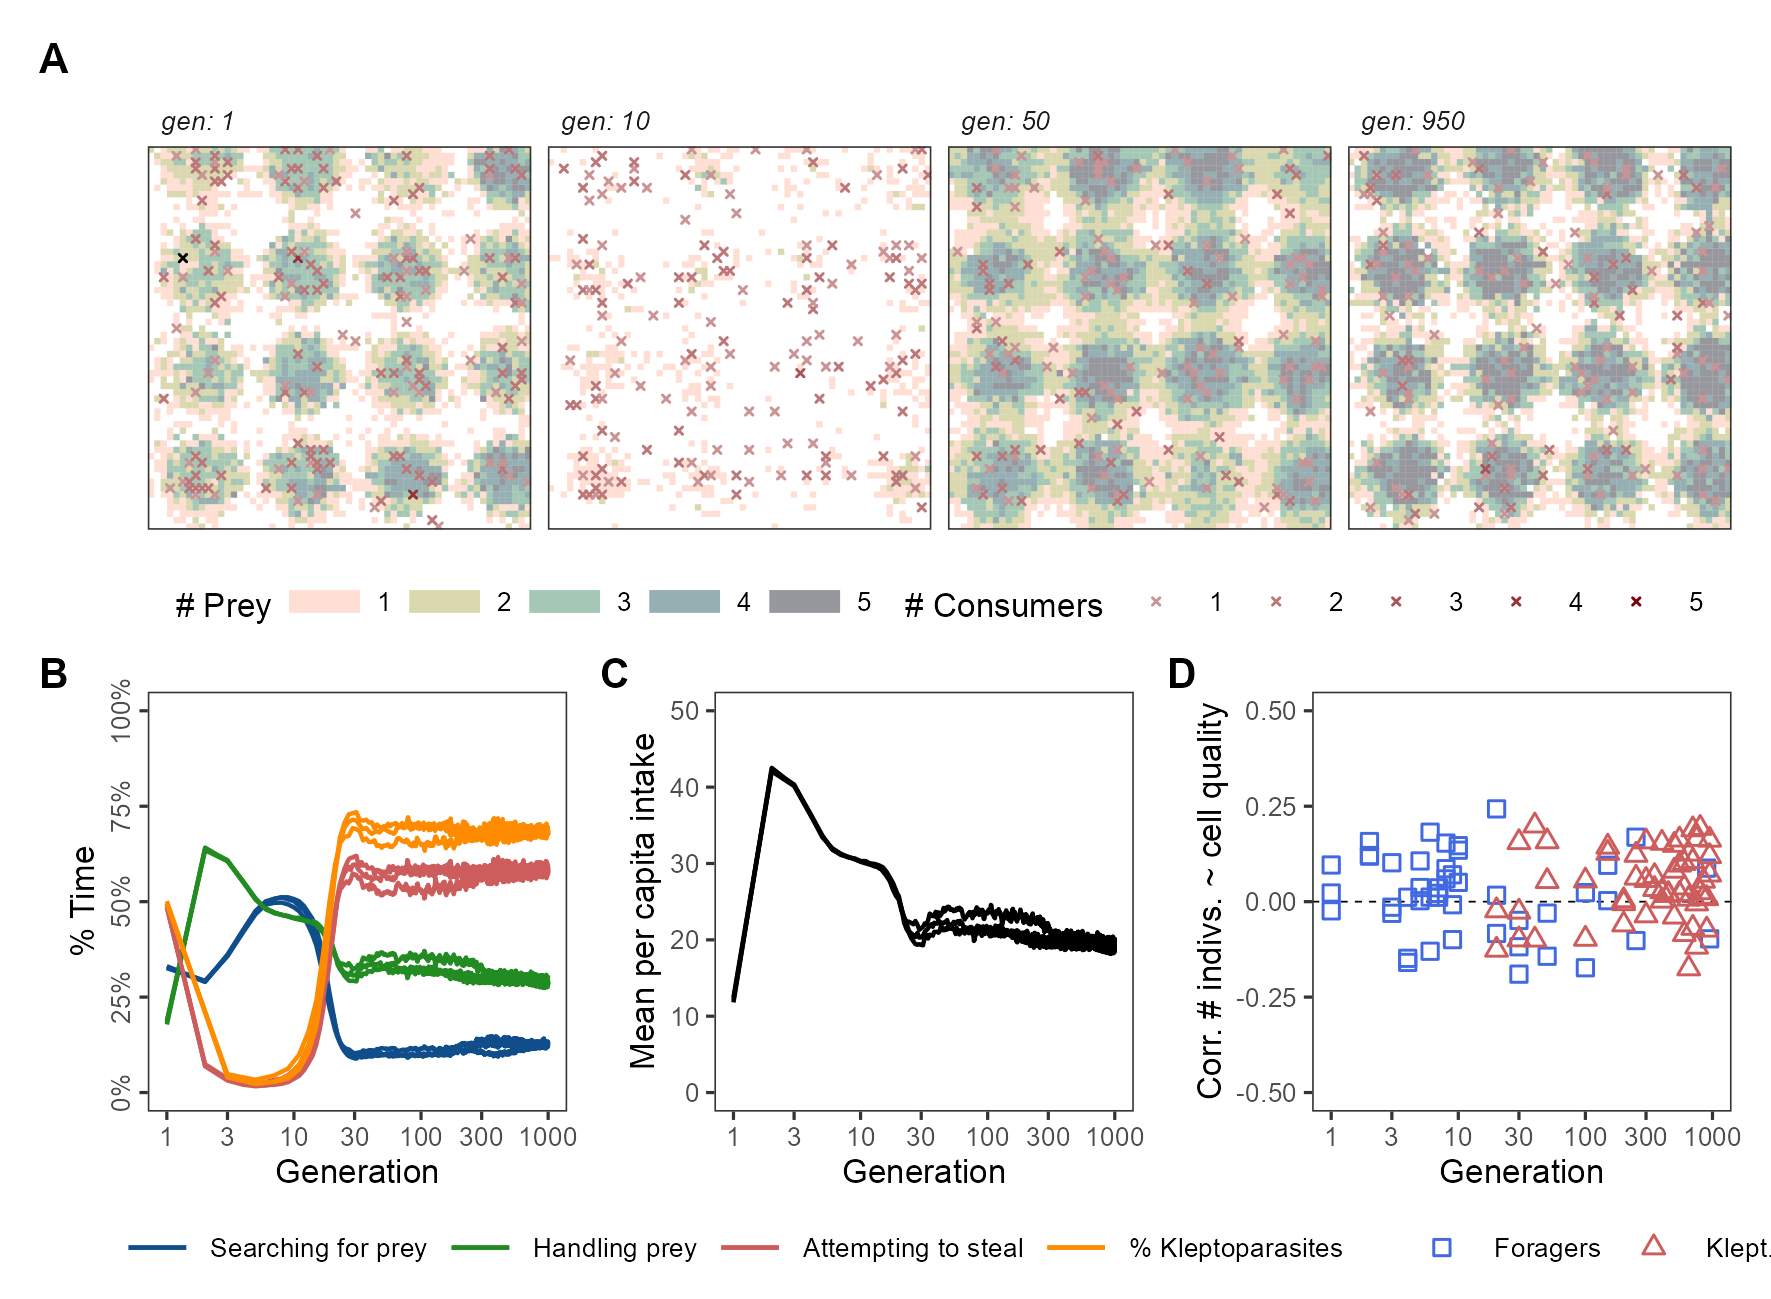
\includegraphics[width=0.9\textwidth]{figures/kleptomove/fig_02.png}
    \caption{
        \textbf{Eco-evolutionary implications of the coexistence of foragers and kleptoparasites following fixed competition strategies in scenario 2.}
        \textbf{(A)} Populations with both foragers and kleptoparasites drastically deplete the initially well-stocked resource landscape by generation 10; however, prey densities recover strongly by generation 50, even beyond the densities in generation 1.
        \textbf{(B)} A surprisingly stable equilibrium between the forager and kleptoparasite strategies is reached within 30 generations, with the relative frequency of kleptoparasites (orange line) first dropping to very low levels but later recovering to reach a high level ($\sim$ 70\%) in all three replicates.
        Consequently, at equilibrium, only about 10\% of individuals are foragers searching for prey, 50\% are kleptoparasites attempting to steal from handlers, and 40\% are handlers processing prey-items (either foragers or kleptoparasites). 
        \textbf{(C)} When kleptoparasites are rare, the population intake rate exhibits the same pattern as in scenario 1, dropping to a lower level with the emergence of kleptoparasites.
        Naturally, there is an increase in the proportion of time spent on stealing attempts (red line -- \textbf{B}), and a corresponding decrease in prey seeking (by searching foragers; blue line -- \textbf{B}), and handling (green line -- \textbf{C}).
        \textbf{(D)} Neither foragers nor kleptoparasites follow the input matching rule, and the correlation of their abundance with cell productivity $r$ is zero at equilibrium.
        Panel \textbf{A} shows a single replicate, while \textbf{B, C, D} and \textbf{D} show three replicates with log-scaled X-axes; all panels are for $r_{max}$ = 0.01.
    }
    \label{klepto_fig_02}
\end{figure}

\begin{figure}[t!]
    \centering
    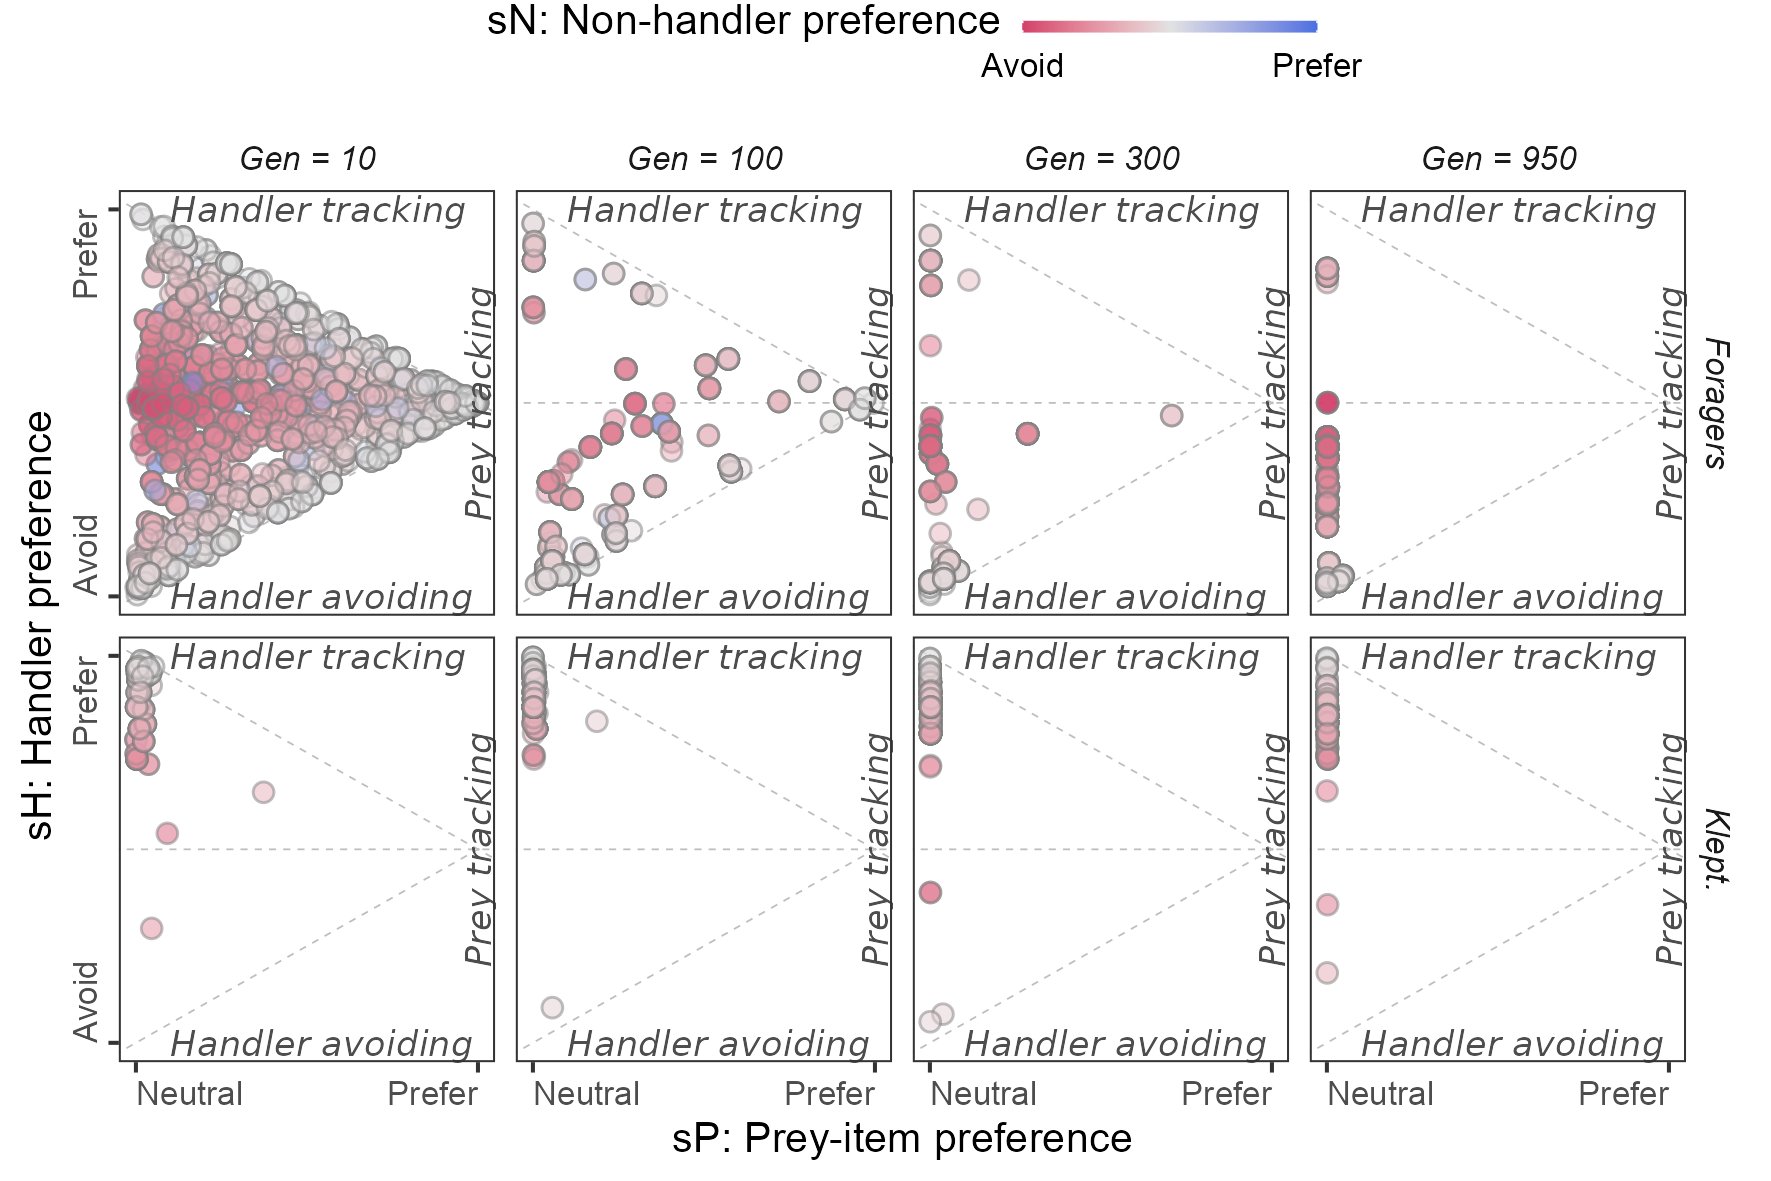
\includegraphics[width=0.9\textwidth]{figures/kleptomove/fig_03.png}
    \caption{
       \textbf{Rapid divergence of movement strategies between foragers and kleptoparasites in scenario 2.}
       In scenario 2, kleptoparasites rapidly diverge (within 10 generations) from foragers in their movement strategy, clustering around sH = 1.0: a handler-tracking strategy.
       This strategy is stably maintained throughout the simulation (G = 100, 300, 950).
       Foragers retain substantial diversity in movement strategies for many generations (see G = 100), but unlike scenario 1, tend to be repelled (relative sH < 0), as well as attracted to handlers (relative sH > 0).
       Over time, foragers adopt a strategy that helps them avoid all other individuals (G = 300, 950).
       A few individuals sporadically adopt a movement strategy associated with the opposite competition strategy; this is most likely due to mutations in the competition strategy, rather than a new movement morph within either foragers or kleptoparasites.
       At the evolutionary equilibrium then, social information (either sH or sN) is the strongest component of all individuals' movement strategies.
       All panels show 2,500 individuals (25\% of total) from the same simulation replicate ($r_{max}$ = 0.01), and earlier generations are ancestors of later generations.
    }
    \label{klepto_fig_03}
\end{figure}

\subsection*{Scenario 3: Condition-dependent Kleptoparasitism}

When individuals are allowed to choose their competition strategy (foraging or kleptoparasitism) based on local environmental cues, the distribution of prey-items is substantially different from the two previous scenarios (Fig.~\ref{klepto_fig_04}A).
Initially, individuals deplete the resource landscape of prey-items within ten generations.
By generation 50, the resource landscape recovers some of the spatial structure of early generations, but prey-item abundances do not match the recovery seen in scenario 2.
This is because unlike scenario 2, individuals search for prey more often and steal less (at or below 25\%; compare Figs.~\ref{klepto_fig_04}B and \ref{klepto_fig_02}B), preventing a full recovery of the resource landscape.
Consequently, mean per-capita intake stabilises (after an initial spike, as in scenarios 1 and 2) within ten generations to a level similar to scenario 1 (Fig.~\ref{klepto_fig_04}C).
While not as strong as predicted by IFD theory, the correlations between consumer abundance and cell productivity are weakly positive (Fig.~\ref{klepto_fig_04}D).

The weak input matching is likely because all individuals prefer to move up gradients of prey density, and towards handlers, which are more likely to be found on resource peaks (Fig.~\ref{klepto_fig_04}E; see also Supplementary Material Fig.~4, 7).
Using conditional foraging strategies, individuals are able to switch between resource types (prey and handlers) depending on which is more profitable \parencite{emlen1966} (`opportunistic kleptoparasitism'; Fig.~\ref{klepto_fig_04}F; see Supplementary Material Fig. 6).
All individuals would choose to steal when handlers are present, even when prey items are more common.
Indeed, about 40\% of individuals would choose to steal even when prey are abundant and there are no handlers at all, showing the prevalence of a `fixed kleptoparasite' clade similar to scenario 2.
In a further parallel with scenario 2, about 70\% of individuals have an intrinsic bias towards kleptoparasitism, i.e., they would by default attempt to steal when there are no cues to inform their decision (Fig.~\ref{klepto_fig_04}F: $P$ = 0, $H$ = 0).

\begin{figure}[t!]
    \centering
    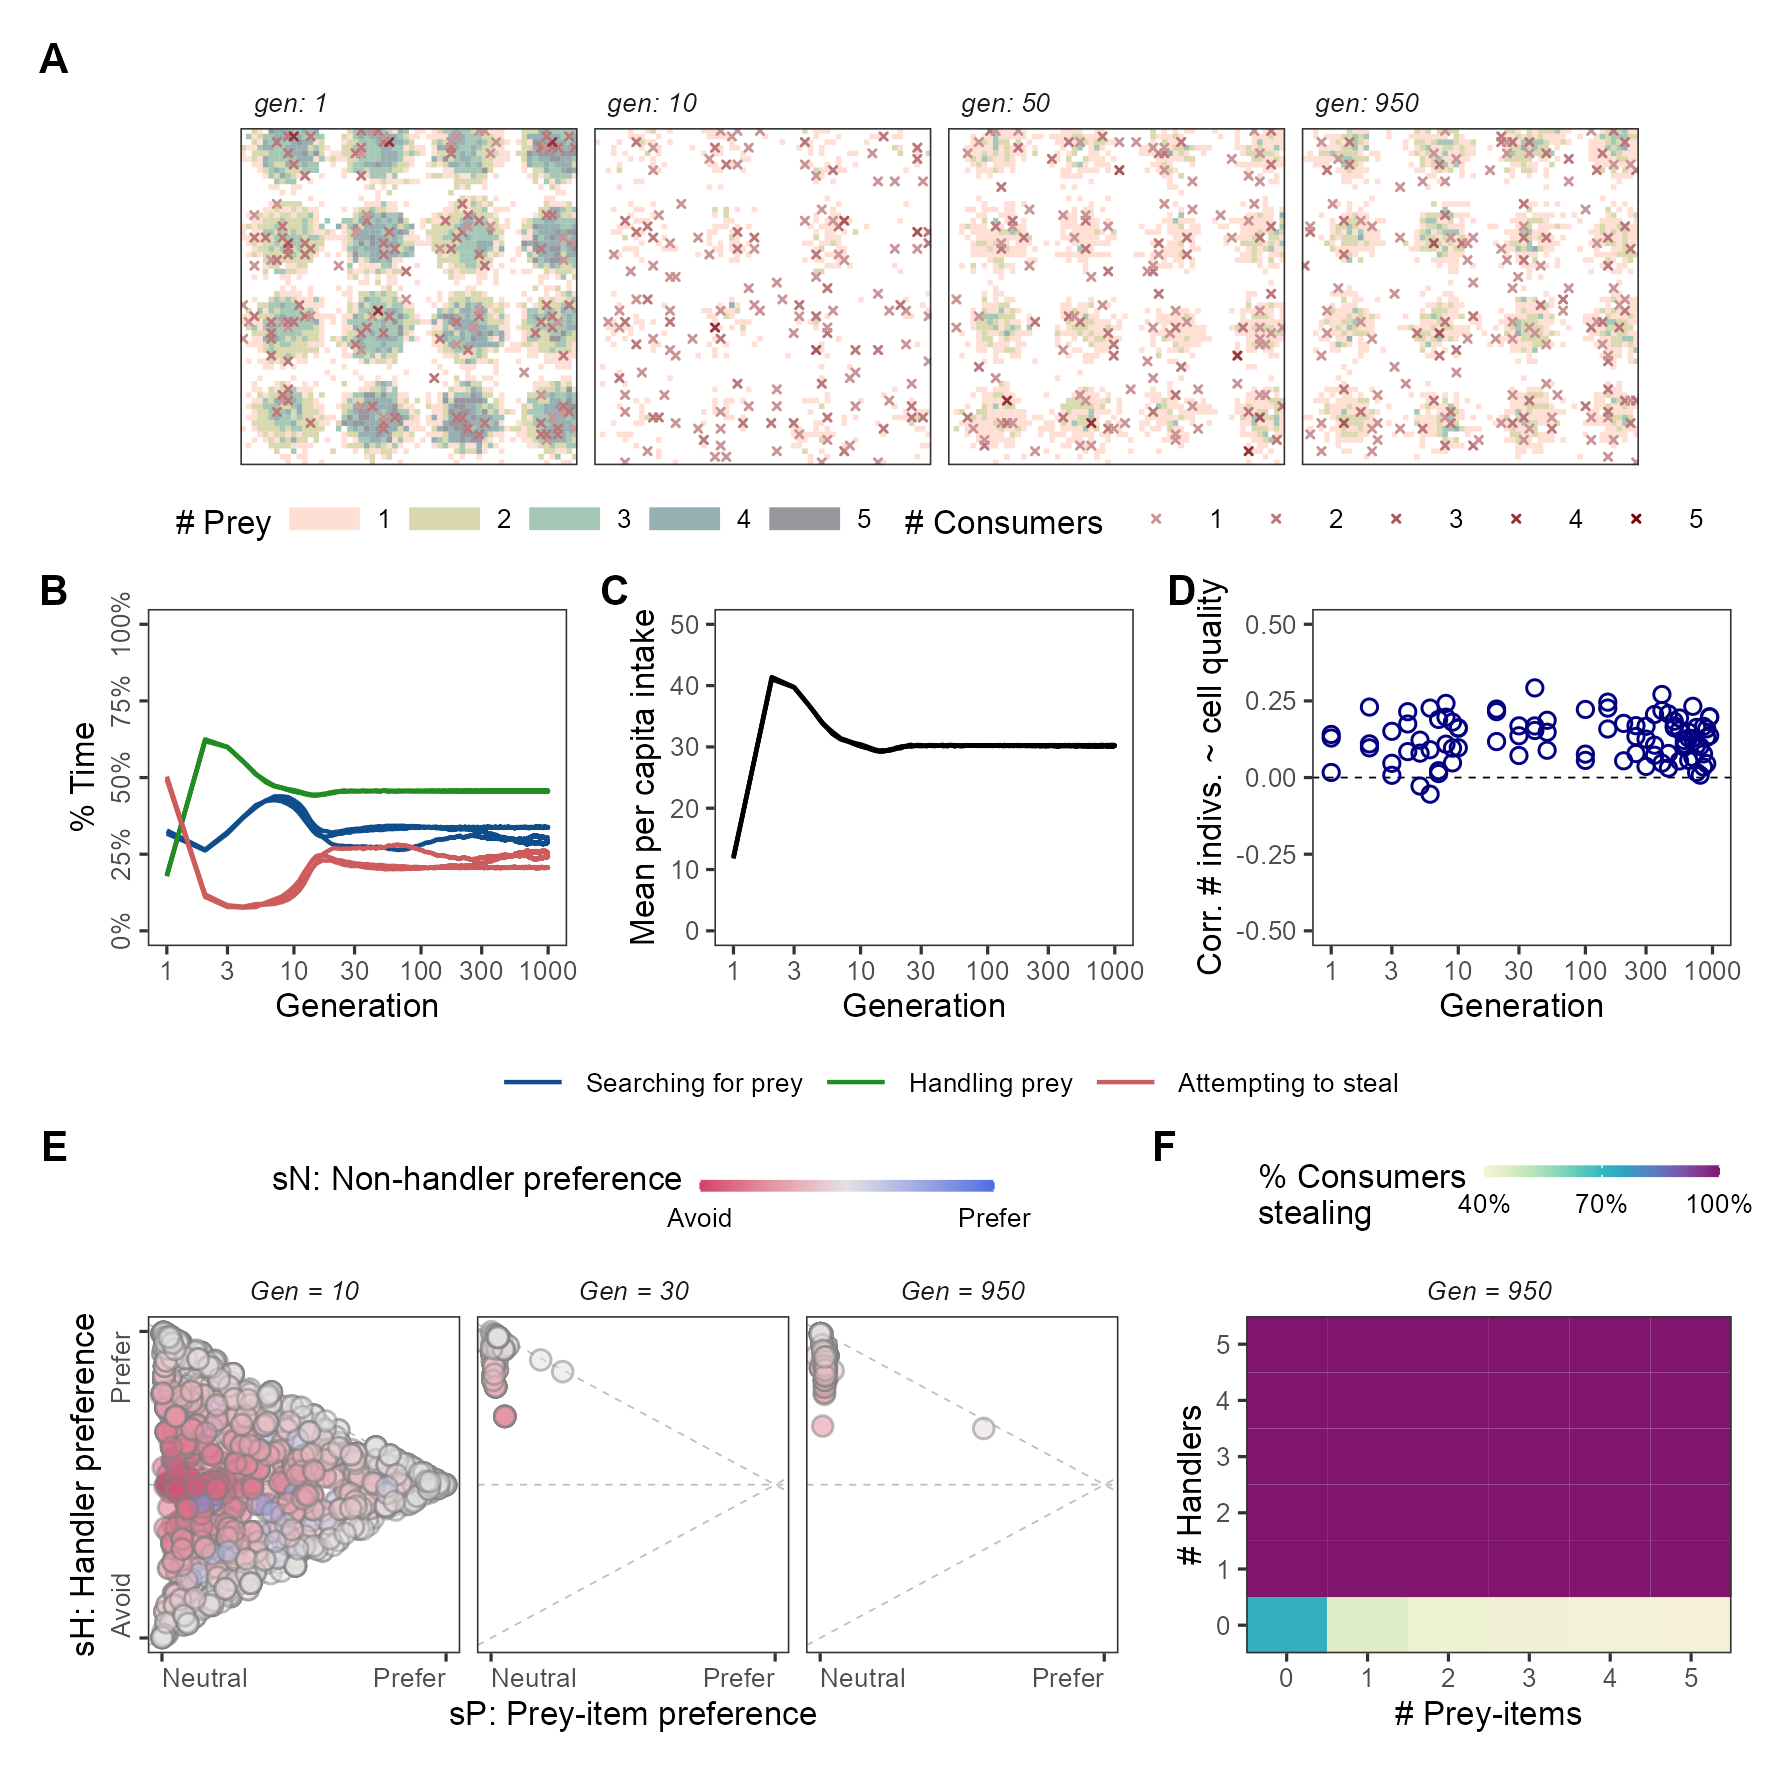
\includegraphics[width=0.9\textwidth]{figures/kleptomove/fig_04.png}
    \caption{
        \textbf{Eco-evolutionary implications of conditional foraging strategies in scenario 3.}
        \textbf{(A)} The initially well-stocked resource landscape is rapidly depleted within 10 generations, yet within 50 generations, prey abundances recover on many cells, though not to the extent of scenario 2.
        The local density of individuals on occupied cells is shown as coloured crosses. 
        \textbf{(B)} By generation 30, the proportion of time spent searching (blue line), handling (green line), and stealing prey (red line) reach an equilibrium that differs somewhat across replicates, but \textbf{(C)} the total intake of the population reaches the same equilibrium value in all three replicates.
        \textbf{(D)} The correlation between the local density of individuals on a cell, and its productivity $r$ is stronger than in scenario 2.
        \textbf{(E)} From an initially high diversity of movement strategies, there is a rapid convergence (within 30 generations) of all individuals to strongly prefer moving towards successful foragers, or handlers, nearly to the exclusion of all other movement cues.
        This handler-tracking strategy once established is maintained (Gen = 300, 950).
        \textbf{(F)} Population competition strategies are more varied. While most individuals will choose to forage as prey density increases, about 40\% of individuals attempt to steal even when prey is abundant and handlers are scarce.
        All individuals will steal when handlers are available.
        Panels \textbf{A, E} show a single replicate, while \textbf{B, C} and \textbf{D} show three replicates, \textbf{F} shows the mean across replicates; all panels are for $r_{max}$ = 0.01.
    }
    \label{klepto_fig_04}
\end{figure}

\subsection*{Movement Strategies on Depleted Landscapes}

Orienting movement towards resources \parencite[][\textit{where to move}]{nathan2008a} can be a challenge in a system with low densities of discrete prey-items, because the local prey \textit{density} may provide very limited information about local \textit{productivity}.
In our model, prey-depletion leads parts of the resource landscape to become `clueless regions' \parencite{perkins1992}, where foragers cannot make directed movements based on prey-item abundances alone, as all neighbouring item abundances are identical (see white areas in Fig.~\ref{klepto_fig_05}A; A1: scenario 1, A2: scenario 2, A3: scenario 3).
At the beginning of all three scenarios, about 75\% of landscape cells have a different number of prey-items from the cells around them; these are primarily cells with an intermediate $r$, which have more prey than peripheral cells of resource peaks, but fewer prey than the central cells.
This proportion rapidly declines to a much lower value within 10 generations in all three scenarios.

The `cluelessness' of the landscapes develops differently across scenarios on evolutionary timescales (Fig.~\ref{klepto_fig_05}B).
In scenario 1, the proportion of cells with a different number of items in the neighbourhood is initially very high (Fig.~\ref{klepto_fig_05}A1).
This proportion rapidly declines to $\sim$25\% within 10 generations, as foragers deplete most prey-items, making most of the landscape a clueless region.
In this context, foragers evolve to move towards handlers, with $>$ 75\% of individuals showing a preference for handlers within 100 generations (Fig.~\ref{klepto_fig_05}B1).
Forager preference for handlers may be explained as the sensing of a long-term cue of local productivity.
Since handlers are immobilised on the cell where they find a prey-item, handler density is an indirect indicator of cell $r$, and due to spatial autocorrelation, also of the $r$ of bordering cells.

Scenario 2 landscapes develop similarly to scenario 1 in early generations (Fig.~\ref{klepto_fig_05}A2).
However, within 50 generations, most cells bear items as extraction is reduced, with differences among cells according to their $r$ (see also Fig.~\ref{klepto_fig_02}A).
Thus $>$ 75\% of cells have a different number of items from neighbouring cells (Fig.~\ref{klepto_fig_05}A2 -- panel \textit{gen: 50}, 5B2).
Unlike scenario 1, the rapid increase in handler preference is driven by kleptoparasites becoming the majority strategy (see above).
Scenario 3 is similar to scenario 2, except that only about half of all cells have a different number of prey-items from neighbouring cells (Fig.~\ref{klepto_fig_05}A3, 5B3).
Here, the rapid evolution of a handler preference in movement decisions cannot be assigned a clear cause, since handlers are both a potential direct resource as well as indirect cues to the location of productive cells.

\begin{figure}[t!]
    \centering
    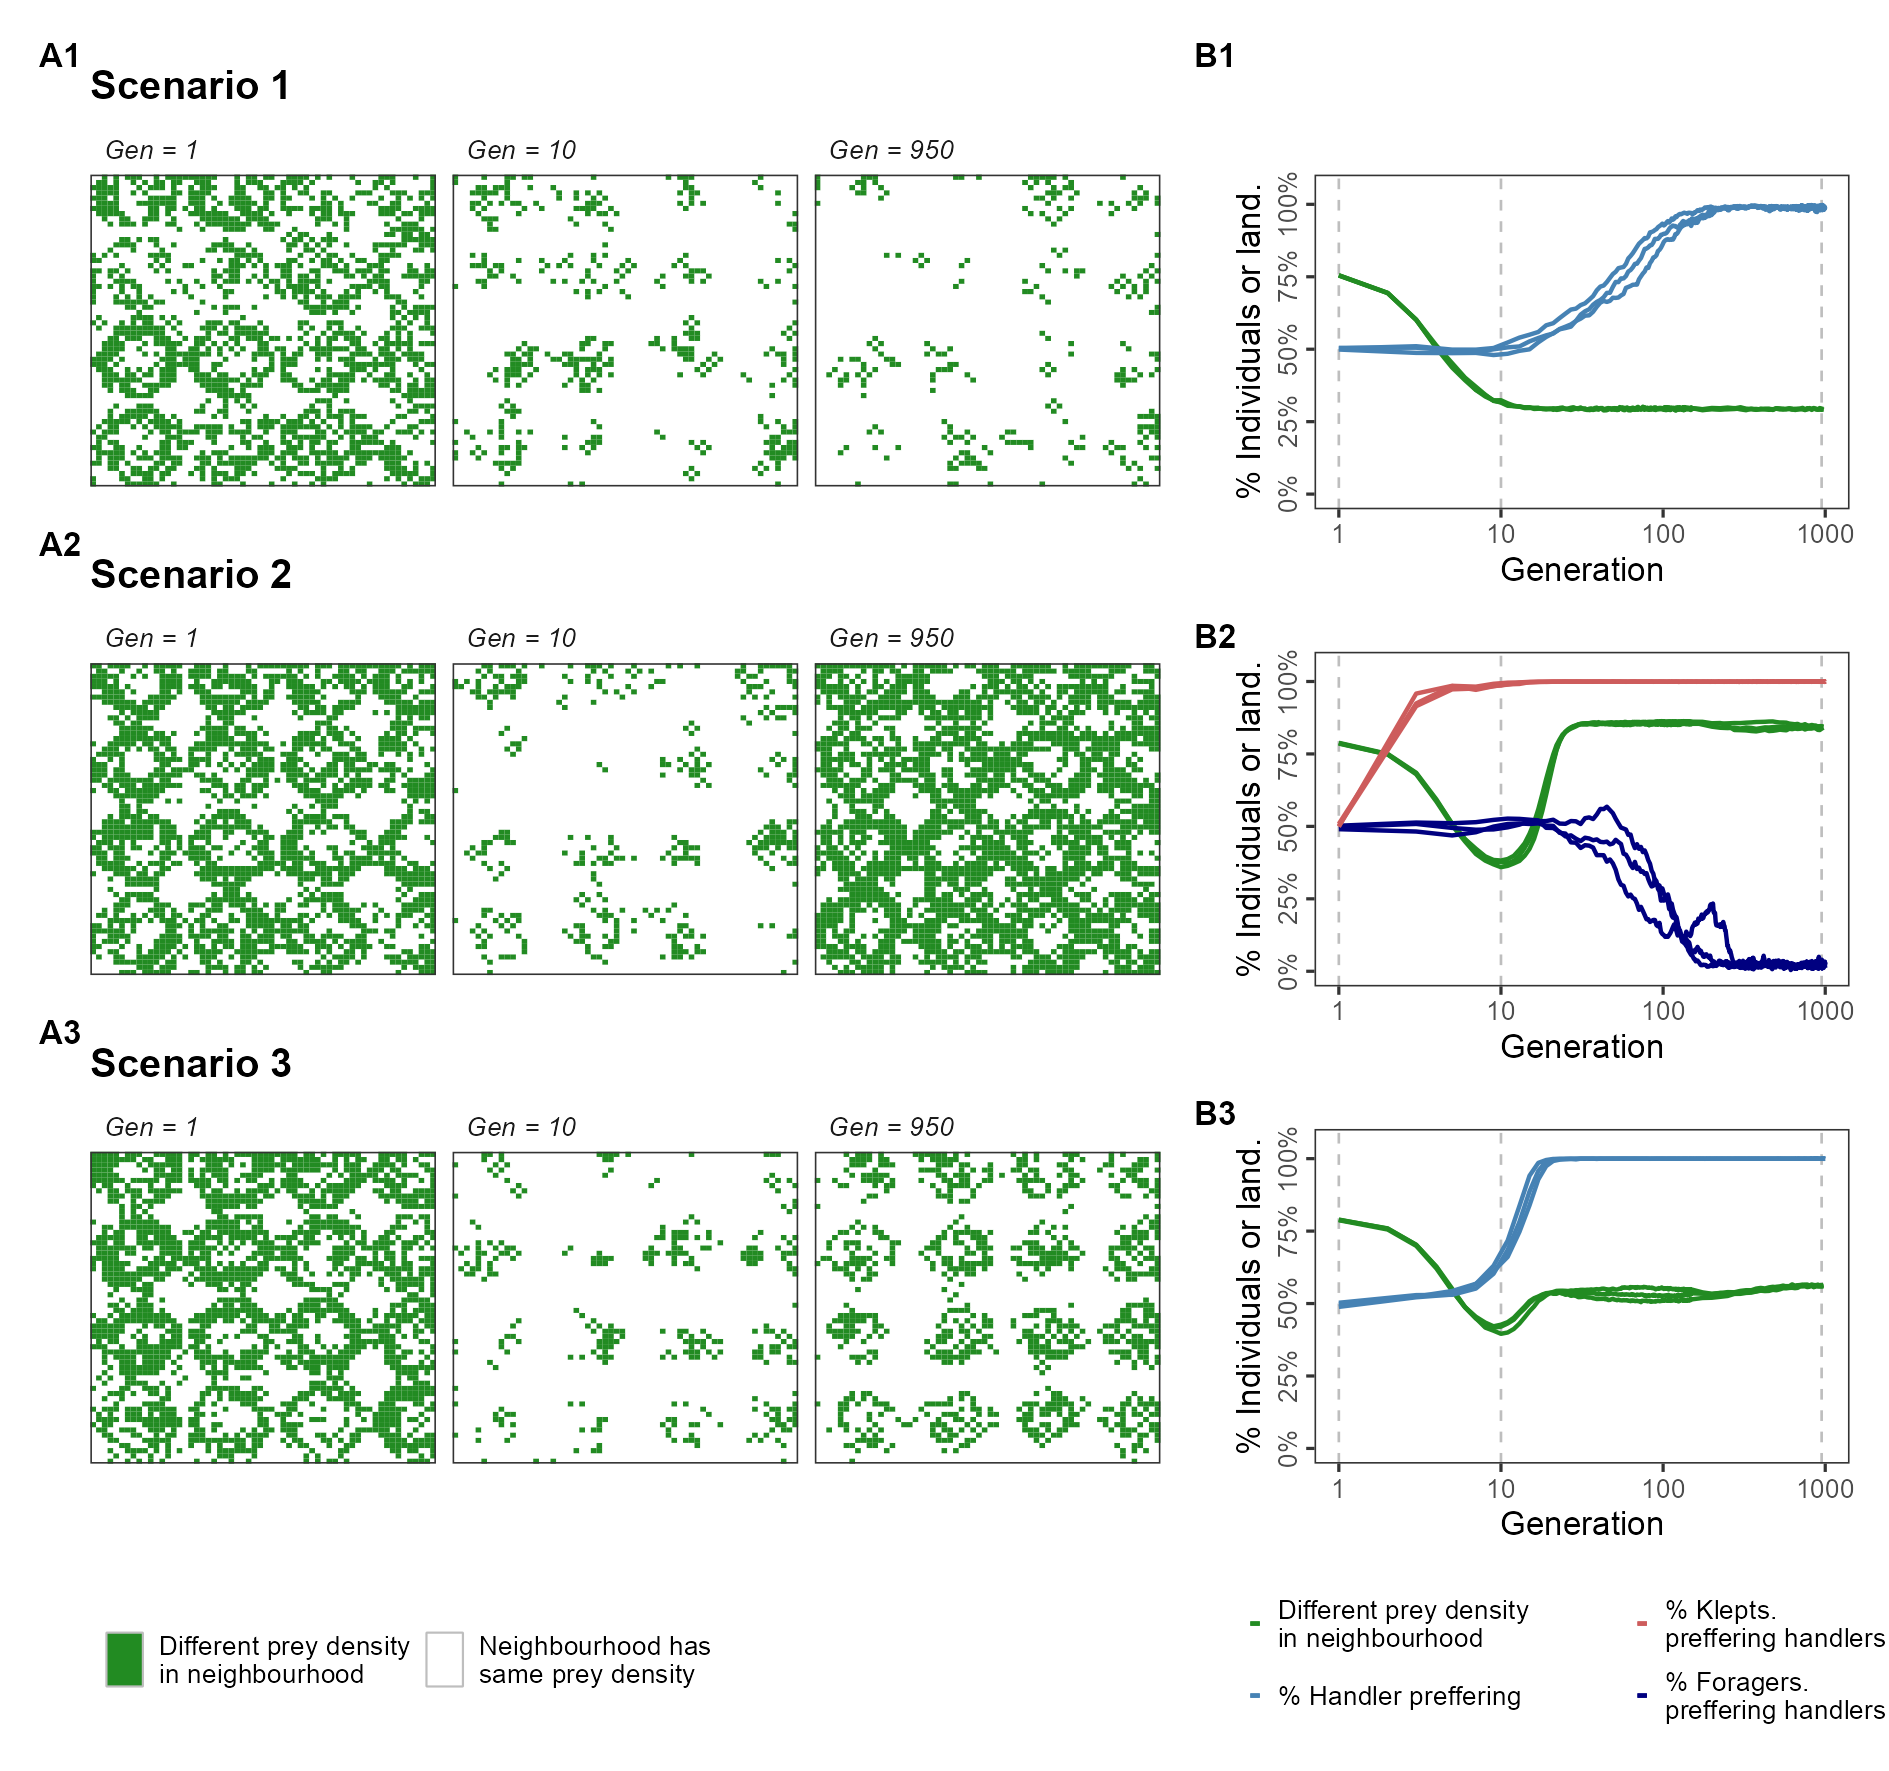
\includegraphics[width=0.9\textwidth]{figures/kleptomove/fig_05.png}
    \caption{
        \textbf{Uninformative prey densities and the evolution of social information as an alternative movement cue.}
        \textbf{(A1, A2, A3)} On cells coloured green, local prey densities are informative for movement, as the central and neighbouring cells have different prey densities.
        While differences in local prey densities provide informative cues for `adaptive' movement in early generations, this is much less true once the resource landscape is depleted of prey-items (depending on the scenario).
        \textbf{(B1, B2, B3)} The proportion of cells where differences in local prey densities provide informative movement cues (green line), and the proportion of individuals preferring to move towards handlers (blue line), whose presence may be used as an alternative cue for movement towards higher-productivity areas of the landscape.
        In \textbf{(B2)} representing scenario 2, this proportion is shown separately for foragers (blue line) and kleptoparasites (red line).
        While panels in \textbf{(A)} show a single representative replicate for $r_{max}$ = 0.01, panels in \textbf{(B)} show three replicates.
    }
    \label{klepto_fig_05}
\end{figure}

\subsection*{Effect of Landscape Productivity}

The prey-item regrowth rate that characterises the peaks of the resource landscape ($r_{max}$) is a measure of the productivity of the resource landscape overall. 
Having thus far focused on scenarios with $r_{max}$ = 0.01 (corresponding to a peak production of 4 food times per consumer lifetime), we find that, not unexpectedly, the value of $r_{max}$ has a marked effect on evolved population activity budgets, mean per capita intake, and even evolved strategies.
The frequency of foraging reduces with $r_{max}$ in scenarios 1 and 3; this is caused by more frequent acquisition of prey-items (as regrowth keeps pace with depletion), which results in a greater frequency of handling rather than foraging.

In scenario 2 however, the frequency of handling is relatively unaffected by increasing $r_{max}$ (Fig.~\ref{klepto_fig_06}A).
The difference between scenarios 2 and 3 has to do with the change in the frequency of kleptoparasitism (Fig.~\ref{klepto_fig_06}B).
In scenario 2, kleptoparasitism forms $>$ 75\% of all activities at low $r_{max}$, and is much more common than in scenario 3 populations at the same regrowth rate.
However, at relatively high $r_{max}$ (0.03), the fixed kleptoparasitic strategy goes extinct.
This is because at high $r_{max}$, forager-prey encounters are more common than kleptoparasite-handler encounters, in both early ($<$ 10) and later generations ($>$ 50).
Consequently, kleptoparasites have relatively much lower fitness than foragers, and do not proliferate.
Thus at high $r_{max}$, a scenario 2 population is nearly identical to a scenario 1 population; while some kleptoparasites may be seen in later generations, these occur most likely due to ephemeral mutations in the forager strategy.

In scenario 3, kleptoparasitism persists at low frequencies even at the highest regrowth rates (Fig.~\ref{klepto_fig_06}B); thus some foragers lose time in extracting items which are then stolen from them.
Consequently, while populations in all three scenarios achieve very similar mean per-capita intakes at low $r_{max}$, at intermediate regrowth rates (0.01, 0.02), conditionally kleptoparasitic populations achieve a higher mean per-capita intake than populations using fixed strategies.
Only at high $r_{max}$, when fixed strategy populations effectively convert to purely forager populations, do they achieve a higher intake than conditional strategy populations (Fig.~\ref{klepto_fig_06}C).

\begin{figure}[t!]
    \centering
    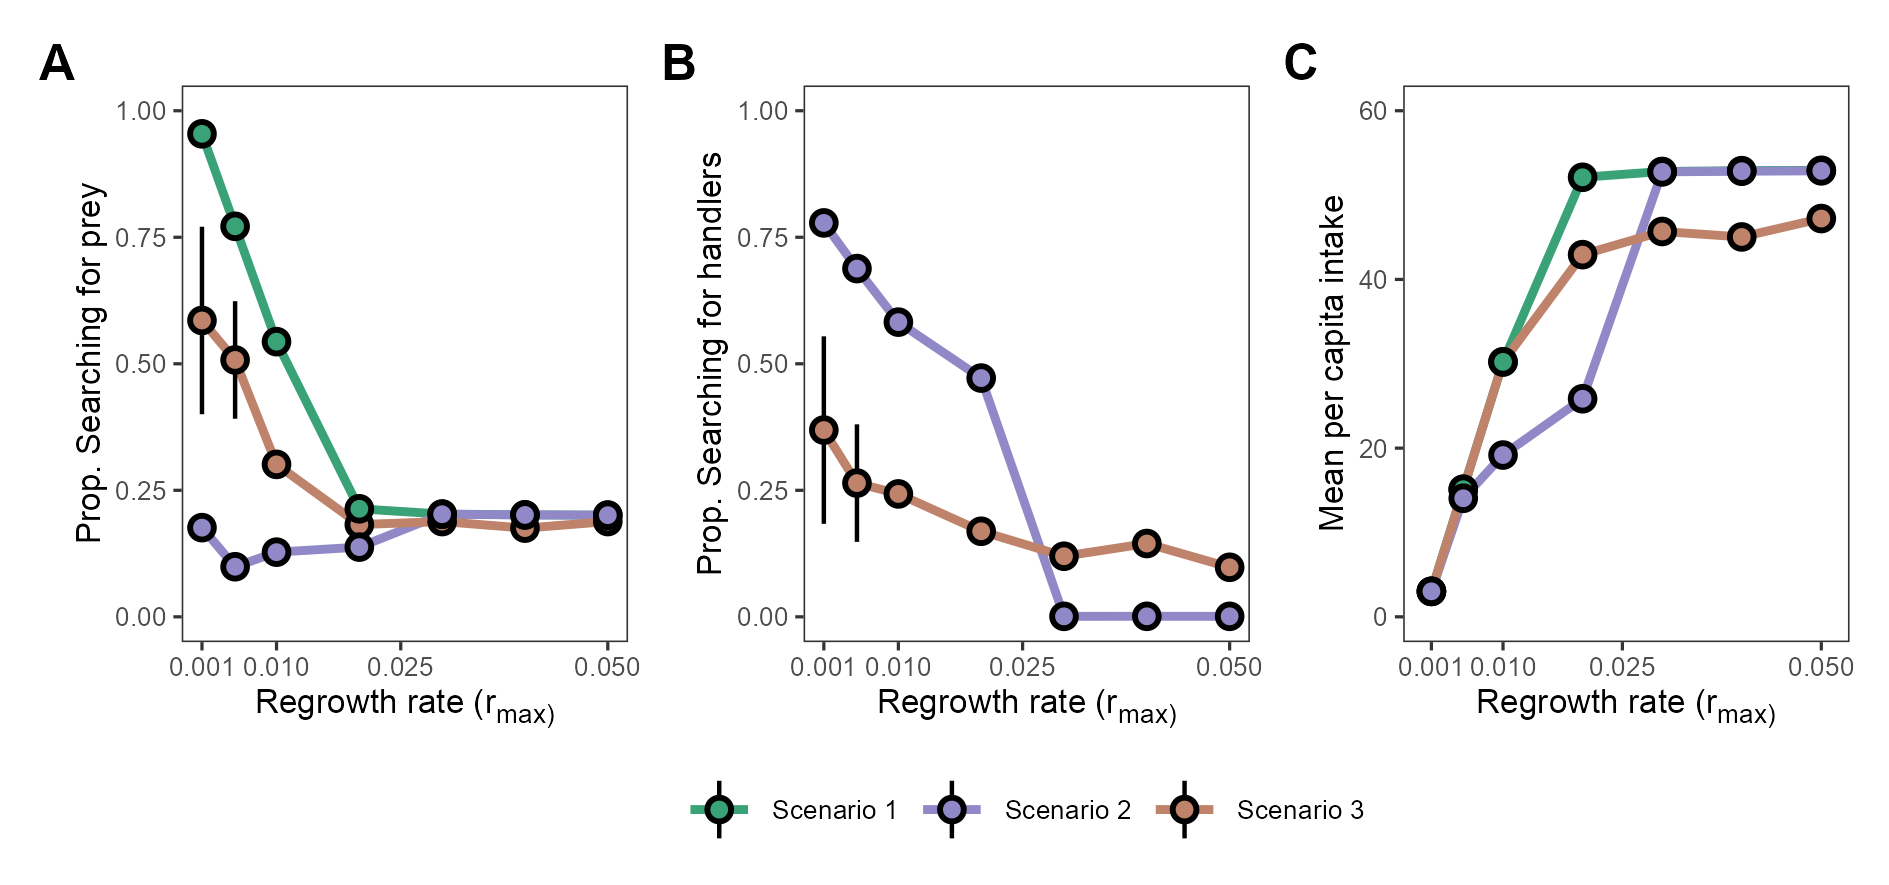
\includegraphics[width=\textwidth]{figures/kleptomove/fig_06.png}
    \caption{
        \textbf{Landscape productivity strongly affects scenario outcomes.}
        \textbf{(A)} The proportion of time spent searching for food decreases with increasing $r_{max}$ in scenarios 1 and 3 but remains relatively stable within scenarios. 
        This is partly due to a higher proportion of time spent handling at higher prey densities. 
        \textbf{(B)} The proportion of time spent searching for handlers (in order to steal prey from them) also decreases with increasing $r_{max}$. 
        In scenario 2, kleptoparasites go extinct for $r_{max}$ values above 0.025. 
        \textbf{(C)} At low productivity, the average intake is similar in all three scenarios. 
        For higher $r_{max}$ values the average intake rate is lowest in scenario 2, until $r_{max}$ is larger than 0.025 and kleptoparasites go extinct (leading to the same kind of population as in scenario 1). 
        At high $r_{max}$, the average intake rate in populations with conditional kleptoparasites (scenario 3) is substantially lower than in populations without kleptoparasitism.
        All panels show conditions at G = 1,000; error ranges where present show standard deviation around values; some error ranges are too small to be visible.
    }
    \label{klepto_fig_06}
\end{figure}

\section*{Contextualising the Outcomes of the Kleptomove Model}

Our spatially-explicit individual-based model implements the ecology and evolution of movement and foraging decisions, as well as resource dynamics, in biologically plausible ways, and offers a new perspective on the distribution of animals in relation to their resources under different scenarios of competition.
%%
First, individuals moving with a limited perception range and competing only by exploitation, evolve movement strategies for both direct and indirect resource cues (prey-items and handlers, respectively).
Regardless, on a resource landscape with discrete prey-items, large areas may become devoid of any movement cues, leading to a mismatch between individual distribution, prey-item distribution, and landscape productivity.
%%
Second, interference competition in the form of kleptoparasitism rapidly establishes itself on landscapes where stealing is more time-efficient than searching for prey, even when such interference is a fixed strategy and kleptoparasites cannot forage for prey.
This rapid increase in kleptoparasitism as a strategy is accompanied by the divergent evolution of movement strategies that favour moving towards handlers, which are the primary resource of the kleptoparasites.
In this sense, obligate kleptoparasites may be thought of as forming a higher trophic level, with handlers as their prey.
%%
Third, when foraging strategy is allowed to be conditional on local cues, \textit{(1)} the population's mean per capita intake is significantly higher than that of a population with fixed strategies, and \textit{(2)} unlike fixed strategy populations, kleptoparasitism as a strategy does not go extinct on high-productivity landscapes.
%%
However, across scenarios, individuals are broadly unable to match the productivity of the resource landscape, contrary to the predictions of IFD based models, which predict input matching for some \parencite{parker1986,holmgren1995,hamilton2002}, or all of the competitive types \parencite{korona1989}.

\subsection*{Comparison with Existing Models}

Existing models of competition and movement impose fixed movement rules on individuals to mimic either ideal or non-ideal individuals \parencite{vickery1991,cressman2006,amano2006b,beauchamp2008,stillman2010,white2018}.
When individual competitive strategies are included in models, they represent differences in competitive ability \parencite[e.g.][]{parker1986,holmgren1995,hamilton2002}, or a probabilistic switch between producing and scrounging \parencite{beauchamp2008}.
In contrast, our model allows individuals' movement (and competition) decisions to be adaptive responses to local environmental cues.
Similar to \textcite{getz2015,getz2016} and \textcite{white2018}, our individuals choose from among the available movement options after weighing the local environmental cues, similar to step selection functions \parencite{fortin2005, avgar2016, white2018}.
Local environmental cues are constantly changing, as we model discrete, depletable prey-items, contrasting with many IFD models \parencite[][]{tregenza1995,amano2006b}.
This allows for a more plausible, fine-scale consideration of exploitation competition, which is often neglected, and allows the cues sensed by individuals to strongly structure the distribution of competitors (see below).

Adaptive responses must have an explicit evolutionary context, and consider multiple generations of the population.
We follow \textcite{beauchamp2008} and \textcite{getz2015} in allowing the cue preferences that decide movement, and variation therein, to be the outcomes of natural selection.
However, instead of using `evolutionary algorithms' \parencite{beauchamp2008,getz2015,getz2016} to `optimise' individual movement rules, we consider a more plausible evolutionary process: \textit{(1)} Instead of allowing the fittest 50\% of the population to replicate, the number of offspring are proportional to individual fitness.
\textit{(2)} The cue preferences are subject to mutations independently, rather than subjecting all preferences of an individual to simultaneous mutation.
\textit{(3)} Finally, we avoided `simulated annealing', which adapts the mutation rate or the mutational step sizes to the rate of evolutionary change.
Instead we drew mutation sizes from a Cauchy distribution, so that most mutations are very small, but large-effect mutations do rarely occur throughout the simulation.
Similarly, rather than determining competition strategy probabilistically or ideally \parencite{vickery1991,beauchamp2008,tania2012}, our individuals' competition decisions are also shaped by selection (in scenarios 2 and 3).

\subsection*{Evolution of Movement Strategies Using Social Information}

In scenario 1, depletion of discrete prey can leave many areas empty of prey-items: in such areas, movement informed by a resource gradient is impossible, and individuals may move randomly \parencite[][]{perkins1992}.
This lack of direct resource cues for locally optimal movement might be among the mechanisms by which unsuitable `matrix' habitats modify animal movement on heterogeneous landscapes \parencite{kuefler2010}.
When individuals do not sense resource gradients, the presence of more successful conspecifics may indicate a suitable foraging spot \parencite[local enhancement;][]{giraldeau1999,beauchamp2008,cortes-avizanda2014}.
The presence of unsuccessful individuals, meanwhile, may signal potential costs from exploitation or interference competition.
This selects for movement strategies incorporating the presence and condition of competitors into individual movement decisions, or \textit{social movement strategies} \parencite[see e.g.][]{guttal2010}.
Consequently, consumer aggregation --- often explained by invoking external costs such as predation \parencite{krause2002,folmer2012} --- could also be the outcome of movement strategies that have evolved to trade competition costs for valuable social information on the underlying spatial structure (here, $r$) of uninformative landscapes \parencite[][]{folmer2010,cortes-avizanda2014}.

\subsection*{Individual Variation in Movement Strategies}

Our movement strategies, comprising preferences for local ecological cues, may lead individuals to move in ways that are potentially unique to each individual.
These strategies may not maximise their intake over short timescales (a few timesteps), but their coexistance implies equivalent fitness overall.
This makes them consistent with prevalent ideas about consistent individual differences in behaviour, or `animal personalities' \parencite{wolf2012,laskowski2013,spiegel2017,shaw2020}.
In scenario 1, the persistence of multiple movement strategies across generations indicates that they have equivalent fitness \parencite[see][]{getz2015}, and that there are multiple ways to navigate a heterogeneous environment \parencite{wolf2010,shaw2020}.
Such differences may help reduce competition as individuals make subtly different movement decisions when presented with the same cues \parencite[][]{wolf2012,laskowski2013}.
Interestingly, scenario 3 has the least individual variation in movement rules, presumably because plasticity in competition strategy reduces the need for such diversification \parencite{pfennig2010}.

Scenario 2 cautions that \textit{(1)} Individual variation may only be evident when accounting for the main driver of movement decisions ($s_H$ or $s_N$; {see Supplementary Material Fig. 8 for scenario 3 as well).
\textit{(2)} Spatial context determines whether individual differences in movement strategy lead to functional variation in movement outcomes.
Subtle variation in relative prey density preferences ($s_P$) could be revealed if individuals were measured in isolation, and could lead to differences in movement paths (given a continuous gradient in prey cues).
However, in natural settings with substantial collective behaviour, different social movement strategies (correlated with foraging competition strategy) would be the primary driver of movement.
Overall, then, \textit{(a)} measuring movement behaviour in settings that correspond to animals' evolutionary context, and \textit{(b)} accounting for movement-competition strategy correlations, are both key when studying how individual differences translate to functional consequences.

\subsection*{Competition Strategies and the Ideal Free Distribution}

IFD models predict that individual movement should result in consumer distributions tracking the profitability of resource patches \parencite{fretwell1970,parker1978}, with dominant competitive types (including kleptoparasites) monopolising the best patches \parencite[][]{parker1986,holmgren1995,hamilton2002}, though \textcite{korona1989} predicts otherwise.
In scenarios 2 and 3, kleptoparasitic individuals unsurprisingly and rapidly evolve to track handlers (a direct resource), while avoiding non-handlers (potential competitors).
However, these evolved rules do not lead kleptoparasites to occupy the best cells as predicted by \citealp{parker1986}, \citealp{holmgren1995}, and \citealp{hamilton2002}.
Across our scenarios (including scenario 1), local population density is only weakly correlated with cell productivity, and is not stronger than if individuals were moving randomly (see Supplementary Material Fig. 1).
In scenario 2, this departure from predictions is driven by the contrasting movement rules of foragers, which evolve to \textit{avoid} handlers as well as non-handlers, both of which might be kleptoparasites \parencite[cryptic interference; seen in interference-sensitive shorebirds][]{bijleveld2012a}.
Thus, foragers likely avoid resource peaks, which are more likely to have handlers \parencite[due to the higher probability of forager-prey encounters][]{parker1986,holmgren1995,hamilton2002}.
Fixed kleptoparasites cannot extract prey themselves, and must move off resource peaks to track and rob handlers \parencite[similar to][]{parker1986}, breaking the link between individual density and productivity.
This shows the pitfalls of simplistically linking current ecological conditions with population distributions without considering competitive strategies or evolutionary history.

\subsection*{Constraints on Competition Strategies}

Foraging strategies involving specialisation on a resource type are expected to be constrained by the availability of that resource. 
Thus kleptoparasitism, seen as a prey-choice problem, should be constrained by the density of targets \parencite{ens1990}.
In scenarios 2 and 3, more kleptoparasitism should be expected with increasing $r_{max}$, as prey and consequently, handlers, are expected to be more abundant.
Instead, kleptoparasitism declines with increasing $r_{max}$, in line with \textcite{emlen1966}, who predicted that the commoner food type (prey) rather than the more efficiently exploited one (handlers) should be preferred.
This prey choice problem, playing out at evolutionary scales, leads kleptoparasites in scenario 2 to go extinct when prey are very common at high $r_{max}$.
At stable population densities, the persistence of fixed kleptoparasitism depends on their intake \textit{relative to foragers}.
Modelling discrete prey-items and individuals in a spatial context, then, leads to the finding that obligate kleptoparasitism is only a viable strategy when forager-prey encounters are less common than kleptoparasite-handler encounters.
Reducing the relative profitability of kleptoparasitism in other ways --- such as imposing a cost on kleptoparasitic attacks for the initiator, or reducing the probability of success (currently, 1.0) --- would also lead to a reduced incidence of kleptoparasitism, and eventual extinction even on less productive landscapes.
In scenario 3, about 40\% of individuals choose to attempt to steal even when prey are available and handlers are not.
This suggests a more realistic proportion of consistently kleptoparasitic individuals among populations with flexible foraging strategies.
Many seabirds, which forage for prey when they are super-abundant, but also readily harass other birds for prey, are a good example \parencite{brockmann1979}.
Finally, comparing across regrowth rates shows why possibly cryptic behavioral complexity should be considered in predictions of the long-term effect of environmental change on populations.
While both scenario 1 and 2 populations appear identical at high $r_{max}$, even a small decrease in environmental productivity could lead to an abrupt drop in per-capita intake --- and potentially, strongly reduced growth or survival --- for fixed strategy populations due to unexpected, emergent kleptoparasitism.

% \subsection*{Comparison with Conceptual Models}

% Classical models of animal movement and foraging largely consider homogeneous populations and environmental conditions, and movements that are made either optimally or at random.
% While these models provide powerful insights, 
% % they also have important drawbacks: individual variation, local environmental conditions, and the mechanisms of movement and decision-making cannot be adequately addressed. 
% % This is the strength of 
% individual-based models such as ours have the advantage that they can accommodate individual variation, local environmental conditions, and the mechanisms of movement and decision-making.
% % : the individual-level perspective can accommodate local circumstances, mechanisms and state variables in considerable depth and detail. 
% Individual-based modeling has the obvious drawback that numerous specific assumptions have to be made, which might not all be founded on empirical evidence, and might seem to limit the generality of the conclusions. 
% Nevertheless, as long as these models are not mistaken for attempts at faithful representations of real systems, their exploration provides valuable perspectives on the conceptual models that have dominated theory in the past. 
% After all, traditional models also include numerous assumptions (the spatio-temporal structure, the timing of events, the distribution and inheritance of traits) that are usually not stated and therefore less visible.
% For the future, we envisage pluralistic approaches, where both types of model are applied to the same research question. 
% Only comparing the outcomes of diverse models will reveal which conclusions and insights are robust, and which reflect peculiarities of the model structure.
% Only such model comparison can tell us whether and when simple models produce general insights, where simple models fail, and when mechanisms can explain initially counterintuitive observations, such as the attraction to competitors that we observed in our study.

\subsection*{Individual-Based Models in Animal Movement Ecology}

Linking individual-based models with empirical data is difficult, and is still rarely used \parencite[see works tailored to management:][]{stillman2010,diaz2021}.
Animal tracking technology is only on the cusp of allowing us to track entire populations (though small ones), and classifying their behaviour at the fine temporal scales of animal decision-making \cite[Nathan et al. in press. \textit{Science}; see e.g.][]{lieber2021, sankey2021}.
Classifying dyadic and collective behaviour from animal tracking is especially challenging \parencite{sankey2021,vissat2021}; this makes the detection of rapid competitive interactions in large populations unlikely.
Instead, experimental approaches may reveal movement strategies that reduce competitive interactions \parencite{vahl2005,vahl2005a,rutten2010, bijleveld2012a}.
However, consistent behaviour in cue-poor captive environments does not always translate to consistency in natural settings with abundant resource cues \parencite{carter2013}.

Animal movement ecology takes an explicitly individual-based approach, centred around individual decisions \parencite{nathan2008a}.
This makes individual-based models a good choice when seeking general insights into the evolutionary ecology of animal movement strategies \parencite[see e.g.][]{getz2015}, whose ultimate causes are otherwise difficult to study empirically.
Modelling mechanistic movement decisions has substantial consequences for ecological outcomes \parencite[e.g.][]{mueller2011,white2018,scherer2020}, yet few individual-based models in animal movement are mechanistic \parencite[see review in:][]{deangelis2019}, and even fewer models include evolutionary dynamics \parencite[but see][]{getz2015,getz2016,netz2021}. 
Yet explicitly modelling both ecological interactions and evolutionary dynamics, as we do here, can reveal surprising outcomes ranging from innovative predator-prey strategies \parencite{netz2021} to sympatric speciation \parencite{getz2016}.

The use of resource- and step-selection functions in mechanistic modelling \parencite[see][]{white2018} gives empirical movement ecologists a familiar starting point in individual-based modelling.
Simulating an animal's potential space-use, conditional on environmental data (similar to our cues), and using selection coefficients estimated from tracking data (our cue preferences), is already accepted in movement ecology, and follows our grid-based approach \parencite{avgar2016,signer2019,avgar2020,fieberg2021}.
It is relatively easy to implement movement decisions in continuous space, by sampling cues at discrete locations and \textit{(1)} choosing among them, or \textit{(2)} translating these cues into a movement distance and turning angle.
The second approach would require more complex functions with more coefficients (preferences), such as neural networks \parencite{mueller2011}, and this could make it difficult to interpret the evolved movement strategies.
Models could implement survival and reproduction (the key ingredients of natural selection), as well as other demographic processes, and reproduction and inheritance can be incorporated in a more realistic manner.

We call for a substantial increase in mechanistic, evolutionary, individual-based modelling in animal movement ecology.
Adding realistic ecological and evolutionary dynamics on top of current empirical work is key to transforming movement ecology into a more applied, predictive discipline.
For example, by allowing habitat selection coefficients from animal-tracking studies to undergo even short-term selection on projected landscapes from climate modelling, such models could help explore population changes in movement strategies.
This approach would require very accurate estimation of the fitness outcomes of movement --- no easy task.
Consequently, individual-based models are not (yet) intended to be `fit' to empirical movement data.
Rather, they can provide valuable perspective on existing population-level models, and could be used to define the envelope of possibilities for how movement strategies could evolve in dynamic environments.

% \section*{Acknowledgments}

% We thank Hanno Hildenbrandt for contributing extensively to the coding of the simulation model \textit{Kleptomove};
% Matteo Pederboni for contributing to the model's development; 
% and members of the Modelling Adaptive Response Mechanisms Group, and of the Theoretical Biology department at the University of Groningen for helpful discussions on the manuscript.
% F.J.W. and C.F.G.N. acknowledge funding from the European Research Council (ERC Advanced Grant No. 789240).
% P.R.G was supported by an Adaptive Life Programme grant made possible by the Groningen Institute for Evolutionary Life Sciences (GELIFES).
% Finally, we thank two anonymous reviewers for helpful suggestions that improved the manuscript.

% \newrefcontext[sorting=nyt]
% \section*{Literature Cited}
% \printbibliography[title={Literature~Cited},heading=none]
% \end{refsection}


\cleardoublepage \begin{refsection}
%************************************************
\chapter{Rapid Evolution of Movement Strategies Following Novel Pathogen Introduction}\label{ch:pathomove}
\chaptermark{Disease \& Movement}
%************************************************

{\noindent \textbf{Pratik R. Gupte}, Gregory F. Albery\textsuperscript{1}, Jakob R.L. Gismann, Amy Sweeny\textsuperscript{2} and Franz J. Weissing}

\graffito{
    
    \textsuperscript{1} Wissenschaftskolleg zu Berlin, Germany.
    \textsuperscript{2} University of Edinburgh, U.K.
}

\section*{Abstract}

\small{
    Animal social interactions are the outcomes of evolved strategies that integrate the costs and benefits of being sociable.
    Using a novel mechanistic, evolutionary, individual-based simulation model, we examine how animals balance the risk of pathogen transmission against the benefits of social information about resource patches, and how this determines the emergent structure of socio-spatial networks.
    We study a scenario in which a fitness-reducing infectious pathogen is introduced into a population which has initially evolved movement strategies in its absence.
    Within only a few generations, pathogen introduction provokes a rapid evolutionary shift in animals' social movement strategies, and the importance of social cues in movement decisions increases.
    Individuals undertake a dynamic social distancing approach, trading more movement (and less intake) for lower infection risk.
    Pathogen-adapted populations disperse more widely over the landscape, and thus have less clustered social networks than their pre-introduction, pathogen-naive ancestors.
    Running epidemiological simulations on these emergent social networks, we show that diseases do indeed spread more slowly through pathogen-adapted animal societies.
    Finally, the mix of post-introduction strategies is strongly influenced by a combination of landscape productivity, the usefulness of social information, and disease cost.
    Our model suggests that the introduction of an infectious pathogen into a population can trigger a rapid eco-evolutionary cascade, rapidly changing animals' social movement strategies, which alters movement decisions and encounters between individuals. 
    In turn, this changes emergent social structures, and our model informs how such change can make populations more resilient to future disease outbreaks.
    Overall, we offer both a modelling framework and initial predictions for the evolutionary and ecological consequences of wildlife pathogen spillover scenarios.

    \bigskip

    {\noindent \large{$\Delta$}} A preprint submitted to \textit{Nature}.
}

\clearpage

\newrefcontext[sorting=ynt]

\lettrine{A}{nimal} sociality emerges from individual decisions that balance the benefits of associations against the costs of proximity or interactions with neighbours \autocite[][]{tanner2012,webber2018,webber2022,gil2018}.
While such associations can inadvertently or deliberately yield useful social information about resource availability \autocite{danchin2004,dall2005,gil2018}, they also provide opportunities for the transmission of parasites and infectious pathogens among associating individuals \autocite[][]{weinstein2018,romano2020,albery2021,cantor2021,romano2021}.
Wildlife pathogen outbreaks affect most animal taxa, including mammals \autocite{blehert2009,fereidouni2019,chandler2021,kuchipudi2022}, birds \autocite{wille2022}, amphibians \autocite{scheele2019}, and social insects \autocite{goulson2015}.
% Balancing the costs and benefits of socialising when deciding , is thus a 
Weighing the potential risk of infection from social interactions against the benefits of social movements --- where to move in relation to other individuals' positions --- is thus a common behavioural context shared by many animal species.
Movement strategies incorporating social information --- the presence and status of neighbours --- can facilitate or reduce spatial associations, and help animals balance the costs and benefits of sociality \autocite{albery2021,gil2018,webber2018,webber2022}.
Animals' social movements link landscape spatial structure, individual distributions, and the emergent structure of animal societies \autocite{gil2018,webber2022,kurvers2014}.
Together, they influence the dynamics of disease outbreaks in animal populations \autocite{white2018a,romano2020,romano2021,keeling2001}, and such outbreaks may in turn have cascading effects on landscape structure and community ecology \autocite{monk2022}.

On ecological timescales, pathogen outbreaks often reduce social interactions among individuals.
This is due to a combination of mortality-induced decreases in population density \autocite[e.g.][]{fereidouni2019,monk2022}, and adaptive behavioural responses by which animals reduce encounters between infected and healthy individuals \autocite{stroeymeyt2018,pusceddu2021,stockmaier2021,weinstein2018}.
The latter case includes self-isolating when infected, or avoiding potentially infectious individuals \autocite{stroeymeyt2018,pusceddu2021,stockmaier2021,weinstein2018}.
However, when pathogens are first introduced into a population, such as during novel cross-species spillover \autocite{kuchipudi2022,chandler2021}, fine-tuned avoidance responses are less likely, as individuals may have no prior experience of cues that indicate infection \autocite{weinstein2018,stockmaier2021}.
Spreading through host-host contacts, pathogens causing chronic infections \autocite{bastos2000,jolles2021,vosloo2009} may instead impose fitness costs, thus selecting against host social behaviour, and hence against social connectivity itself \autocite{altizer2003,cantor2021,romano2021,poulin2021,ashby2022}.

% Yet introductions of novel pathogens into wildlife mostly come to light when they result in mass mortality events \autocite{fey2015,wille2022}.
Yet novel pathogen introductions are primarily studied for their immediate demographic \autocite{fey2015}, and potential medical \autocite{wille2022,chandler2021,kuchipudi2022,levi2012} and economic implications \autocite[][]{keeling2001,goulson2015,jolles2021}, with host evolutionary dynamics (and especially changes in sociality) mostly ignored.
This is presumably because the evolution of pathogen host traits, and moreover complex behavioural traits such as sociality, is expected to be slow and not immediately relevant.
Since important aspects of animal ecology, including the transmission of foraging tactics \autocite{klump2021} and migration routes \autocite{jesmer2018,guttal2010}, depend on social interactions, it is necessary to understand the long-term consequences of pathogen introductions for animal societies.
Climate change is only expected to make novel pathogen introductions more common \autocite{sanderson2020,carlson2022a}, making such studies more urgent.

Theory suggests that animal sociality evolves to balance the value of social associations against the risk of pathogen transmission \autocite[][]{bonds2005,prado2009,ashby2022}.
However, analytical models often reduce animal sociality to single parameters, while it actually emerges from individual decisions conditioned on multiple internal and external cues.
Social decision-making and movement often also vary among individuals \autocite{tanner2012,wolf2012,spiegel2017,gartland2021}, but analytical models are unable to include individual differences in sociability.
Epidemiological models based on contact networks can incorporate individual variation in social behaviour by linking these differences to positions in a social network \autocite{white2017,albery2021,albery2020}.
Yet network models often cannot capture fine-scale feedbacks between individuals' social and spatial positions \autocite{albery2021,albery2020}, nor spatial variation in infection risk \autocite{albery2022}, making such models sensitive to both the network formation process, and to sampling biases in empirical data collection \autocite[][]{white2017}.

Mechanistic, individual-based simulation models (IBMs) suggest themselves as a natural solution; they can incorporate substantial ecological detail, including explicit spatial settings \autocite{deangelis2019}, and detailed disease transmission \autocite{white2018, scherer2020,lunn2021,white2018a}.
Individual-based models hitherto haved focused on immediate epidemiological outcomes, such as infection persistence, and do not have an evolutionary component \autocite{white2018,scherer2020,lunn2021}.
Incorporating an evolutionary component to movement-disease IBMs could allow predictions on important feedbacks between the ecological outcomes of infectious disease and the consequences for the evolution of host behaviour \autocite{cantor2021}.
This could include the emergence of tradeoffs in the costs and benefits of sociability \autocite{gartland2021}, with cascading ecological and social effects \autocite{monk2022,spiegel2017,tanner2012,webber2022}.
The range of animal taxa at risk from a wide array of pathogens and parasites \autocite{carlson2022a,sanderson2020} makes it important to conceive of models that can capture the key features of diverse host-pathogen dynamics and offer broad conceptual insights \autocite{white2018a,white2018}.

We built a model that seeks to capture the essential elements of pathogen (or parasite) transmission among animals foraging on patchily distributed resources --- this is a common behavioural context shared by many potential host species \autocite{white2018a,white2018}.
We examined the eco-evolutionary consequences of the introduction of a pathogen into a novel host population \autocite[such as during cross-species spillover:][]{blehert2009,bastos2000,wille2022,fereidouni2019,scheele2019,sanderson2020,carlson2022a,kuchipudi2022,monk2022}.
In our evolutionary, spatial, individual-based simulation, we modelled the repeated introduction of an infectious pathogen to populations that had already evolved foraging movement strategies in its absence.
Our model could be conceived as an abstract representation of, among others, spillovers of foot-and-mouth disease from buffalo to impala \autocite{bastos2000,vosloo2009}, or sarcoptic mange from llamas to vicu\~nas \autocite{monk2022}, current and historic spread of avian influenza among sea- and wading bird species \autocite{globconsorth5n82016,wille2022}, or SARS-CoV-2 from humans to deer \autocite{chandler2021,kuchipudi2022}.

We compared how social information was used in movement strategies evolved before and after pathogen introduction, and the ecological outcomes for individual intake, movement, and associations with other foragers.
Using both IBMs and network epidemiological models \autocite{wilber2022,stroeymeyt2018,white2017,bailey1975}, we examined whether pathogen-risk adapted populations were more resilient to the spread of infectious disease than their pathogen-risk naive ancestors.
We also investigated the effect of landscape productivity and the cost of infection, which are both expected to influence the selection imposed by pathogen transmission \autocite{ezenwa2016,almberg2015,hutchings2000}.
Overall, we provide a theoretical framework broadly applicable to novel host-pathogen introduction scenarios, and demonstrate the importance of including evolutionary dynamics in movement-disease models.

\section*{The Pathomove Model of Novel Pathogen Introduction}

We implemented an individual-based simulation model to represent foraging animals (`foragers') seeking discrete, immobile, depleteable food items (see \textit{SI Appendix Fig. S1 -- S2}) \autocite{spiegel2017,gupte2021a}.
Food items are distributed over a two-dimensional, continuous-space resource landscape with wrapped boundaries (a torus).
Our model, similar to previous eco-evolutionary individual based models \autocite{getz2015, netz2021, gupte2021a}, has two distinct timescales: (1) an ecological timescale comprising of \textit{T} timesteps that make up one generation ($T$ = 100 by default), and (2) an evolutionary timescale consisting of 5,000 generations (G).
At the ecological timescale, individuals sense local counts of food items and competitors, move according to inherited movement strategies, and forage for food.
At the same timescale, individuals that carry an infectious, fitness-reducing pathogen, may, when in close proximity with uninfected individuals, pass on the pathogen with a small probability (see \textit{Pathogen Transmission and Disease Cost}).
At the evolutionary timescale, individuals reproduce and transmit their movement strategies (see \textit{Starting Location and Inheritance of Movement Rules}) to the their offspring. The number of offspring is linked both to individuals' success in finding and consuming food items, and to the duration that they were infected by the pathogen at the ecological timescale.
The model was implemented in R and C++ using Rcpp \autocite{rcoreteam2020,eddelbuettel2013} and the \textit{Boost.Geometry} library for spatial computations (\textit{www.boost.org}); model code is at \textit{github.com/pratikunterwegs/pathomove}.

\subsection*{Distribution of Food Items}

Our landscape of 60 $\times$ 60 units contains 1,800 discrete food items, which are clustered around 60 resource `kernels', for a resource density of 0.5 items per unit\textsuperscript{2} (see \textit{SI Appendix Fig. S1 -- S2}).
% Food items are initialised to become available after some $t$ timesteps, where $t$ is drawn from a Poisson distribution with a mean of 10 (10\% of the regeneration time; see below).
This prevents synchronicity in the availability and regeneration of food items.
Each available food item can be sensed and harvested by foraging individuals (see below).
Once harvested, another food item is regenerated at the same location after a fixed regeneration time R, which is set at 50 timesteps by default; alternative values of 20 and 100 timesteps represent high and low productivity landscapes respectively.
Food item regeneration is delinked from population generations.
Thus the actual number of available food items is almost always in flux.
In our figures and hereafter, we chose to represent R as the number of times a food item would regenerate within the timesteps in a single generation $T$ (default = 100), resulting in R values of 1, 2, and 5 for regeneration times of 100, 50 (the default), and 20 timesteps.
Items that are not harvested remain on the landscape until they are picked up by a forager.
Each food item must be processed, or `handled', by a forager for $T_H$ timesteps (the handling time, default = 5 timesteps) before it can be consumed \autocite{ruxton1992,gupte2021a}.
The handling time dynamic is well known from natural systems in which there is a lag between finding and consuming a food item \autocite{ruxton1992}, and may be caused by the need to extract edible portions from inedible structures, such as mussels from their shells, or seeds from their casings.

\subsection*{Individual Foraging and Movement}

Individuals forage in a randomised order, harvesting the first available food item within their movement and sensory range ($d_S$ = $d_M$, a circle with a radius of 1 unit (see \textit{SI Appendix Fig. S1 -- S2}).
Once harvested, the item is no longer available to other individuals, leading to exploitation competition among nearby foragers.
Furthermore, the location of the item also yields no more cues to other foragers that an item will reappear there, reducing direct cues by which foragers can navigate to profitable clusters of food items.
Individuals that harvest a food item must handle it for $T_H$ timesteps (default = 5 timesteps), while all individuals not handling a food item are considered idle \autocite{ruxton1992,gupte2021a}.
As handlers are immobilised at the location where they encountered food, they may be good indirect indicators of the location of a resource cluster (`social information') \autocite[][]{danchin2004,romano2020,gupte2021a}.
Once individuals finish handling a food item, they return to the non-handling, searching state.

Our model individuals move in small, discrete steps of fixed size ($d_M$ = 1 unit).
<<<<<<< HEAD
Each step is chosen based on the individuals' assessment of local environmental cues, and this assessment is made using evolved movement strategies \autocite[as in][]{netz2021,gupte2021a}.
First, individuals scan their current location, and five equally spaced points around their position, at a distance of 1 unit for three cues ($d_S$, see \textit{SI Appendix Fig. S1 -- S2}): the number of food items ($F$), the number of foragers handling a food item (`handlers': $H$) and the number of idle foragers not handling a food item (`non-handlers': $N$).
Individuals assign a suitability \autocite[see][]{netz2021,gupte2021a} to their current position and each of the five locations, using their inherited preferences for each of the cues: $S = s_FF + s_HH + s_NN$ + $\epsilon$.
=======
Each step is chosen based on the individuals' assessment of local environmental cues, and this assessment is made using evolved movement strategies \citep[as in][]{netz2021,gupte2021a}.
First, individuals scan their current location, and five equally spaced points located on the arc of a circle with a radius of 0.5 units ($\sim$1\% of the landscape's side).
around their position, at a distance of 1 unit for three cues ($d_S$, see \textit{Supplementary Information}): the number of food items ($F$), the number of foragers handling a food item (`handlers': $H$) and the number of idle foragers not handling a food item (`non-handlers': $N$).
Individuals assign a suitability \citep[see][]{netz2021,gupte2021a} to their current position and each of the five locations, using their inherited preferences for each of the cues: $S = s_FF + s_HH + s_NN$ + $\epsilon$.
>>>>>>> 8d43b47ddc128b0830158c7f25ae286fb9050a49
The preferences $s_F$, $s_F$, and $s_N$ for each of the three cues are heritable from parents to offspring, while $\epsilon$ is a very small error term drawn for each location, to break ties among locations.
The values of each of the cue preferences \emph{relative to each other} determine individuals' movement strategies \autocite{gupte2021a}.
All individuals move simultaneously to the location to which they have assigned the highest suitability (`step selection') \autocite[akin to step-selection;][]{fortin2005}; this may be their current location, in which case individuals are stationary for that timestep.
Since individuals may differ in their inherited preferences for each of the three cues, two individuals at the same location may make quite different movement decisions based on the same local cues.
Handlers, however, are considered immobile and do not make any movement decisions.

\subsection*{Pathogen Transmission and Disease Cost}

We modelled circumstances that are expected to become increasingly common due to rapid global changes; the population evolves for $3/5$\textsuperscript{th} of the simulation (until G = 3,000; of 5,000) in the absence of a pathogen, after which a pathogen is introduced in each generation until the end of the simulation (G = 5,000).
Our model captures some essential features of pathogen or parasite transmission among animals \autocite{white2017}: the pathogen may transmit from infected host individuals to their susceptible neighbours with a per-timestep probability $p$ of 0.05.
This transmission is only possible when the two individuals are within a the transmission distance, $d_\beta$.
For simplicity, we set $d_\beta$ to be the movement range (1 unit).
Once transmitted, the pathogen is assumed to cause a chronic disease which reduces host energy stores by a fixed amount called $\delta E$ in every following timestep; $\delta E$ is set to 0.25 by default (alternative values: 0.1, 0.5).
Since novel pathogen introductions can periodically re-occur in natural environments \autocite{jolles2021,bastos2000,vosloo2009,almberg2015,goulson2015,wille2022,carlson2022a}, we set up our model such that the pathogen was introduced to 4\% of individuals in each generation (N = 20; `primary infections').
This is necessary to kick-start the pathogen-movement eco-evolutionary feedback dynamics, and populations may indeed repeatedly acquire novel pathogens (or strains) through external sources, such as infected individuals of other spatially overlapping species \autocite[e.g.][]{kuchipudi2022,wille2022,chandler2021,vosloo2009,bastos2000,monk2022,keeling2001,carlson2022a}.
For completeness, we also considered scenarios in which novel pathogen introductions only occur sporadically in the generations after the initial event, rather than in every generation (see \emph{SI Appendix}).

\subsection*{Starting Location and Inheritance of Movement Rules}

For simplicity, we considered a population of haploid individuals with discrete, non-overlapping generations, and asexual inheritance.
At the end of the parental generation, the net lifetime energy of each individual was determined as the difference of the total energy gained through food intake and the energy lost through infection. 
In the \textit{SI Appendix}, we also consider an alternative implementation in which potential immune resistance against the pathogen requires a certain percentage of individual intake, reducing the value of each food item.
The parental population produces an offspring population (of the same size) as follows: to each offspring, a parent is assigned at random by a weighted lottery, with weights proportional to lifetime net energy (an algorithm following the replicator equation) \autocite{hofbauer1988,hamblin2013}.
This way, the expected number of offspring produced by a parent is proportional to the parent's lifetime success \autocite{hofbauer1988}.
The movement decision-making cue preferences $s_F$, $s_H$, and $s_N$ are subject to independent random mutations with a probability of 0.01.
The mutational step size (either positive or negative) is drawn from a Cauchy distribution with a scale of 0.01 centred on zero.
Thus, while the majority of mutations are small, there can be a small number of very large mutations.
As in real ecological systems, individuals in the new generation are intialised around the location of their parent (within a standard deviation of 2.0), and thus successful parents give rise to local clusters of offspring (see an alternative implementation in \textit{SI Appendix}).

\subsection*{Model Output}

To understand the evolution of movement strategies, and especially how individuals weighed social information, we recorded the population's evolved cue preferences in every second generation, and interpreted them using the `behavioural hypervolume' approach \autocite{bastille-rousseau2019}.
We classified individuals based on how they used social information --- the presence and status of competing foragers --- into four social movement classes: (1) agent avoiding, if $s_H, s_N < 0$, (2) agent tracking, if both $s_H, s_N > 0$, (3) handler tracking, if $s_H > 0, s_N < 0$, and (4) non-handler tracking, if $s_H < 0, s_N > 0$.
We calculated the relative importance of social cues --- $H, N$ --- to each individual's movement strategy as $ SI_{imp} = (|s_H| + |s_N|) / (|s_H| + |s_N| + |s_F|)$, with higher values indicating a greater importance of social cues.

Animal movements and foraging distributions provide opportunities for between-individual associations, which usually have a spatial context.
Associations which depend on spatial proximity can be captured at the individual- and population-level by proximity-based animal social networks \citep{whitehead2008,farine2015}.
Social networks measured from empirical studies have been broadly informative about the structure of animal societies, and the consequences of this structure for animal culture, such as the learning of migration routes or foraging skills \citep{aplin2012,aplin2013,cantor2021}, and for disease transmission \citep{stroeymeyt2018,albery2021,cantor2021}.
%%
We created a proximity-based adjacency matrix by counting the number of times each individual was within the sensory and pathogen transmission distance $d_\beta$ (= $d_S, d_M$ = 1 unit) of another individual \citep{whitehead2008,wilber2022}.
We transformed this matrix into an undirected social network weighted by the number of pairwise encounters: in a pairwise encounter, both individuals were considered to have associated with each other \citep{white2017}.
The strength of the connection between any pair was the number of times the pair were within $d_\beta$ of each other over their lifetime.
%%
We logged encounters and constructed social networks after every 10\% of the total generations (i.e., every 500\textsuperscript{th} generation), and at the end of the simulation.
We constructed adjacency matrices using Rcpp \citep[][]{eddelbuettel2013}, and converted them to networks using the \textit{igraph} \citep{csardi2006} and \textit{tidygraph} \citep{pedersen2020} libraries for R.
We omitted ephemeral pairwise associations with a weight $<$ 5.

We plotted the mix of social information-based movement strategies evolved across generations in each parameter combination.
Focusing on our default scenario ($\delta E$ = 0.25, R = 2), we visualised the mean per-capita distance moved, mean per-capita intake, and mean per-capita encounters with other foragers.
We examined how the three main social movement strategies --- agent avoidance, agent tracking, and handler tracking --- changed in frequency over generations.
We also examined differences among strategies in the movement distance, associations with other agents, and frequency of infection, after they had reached an eco-evolutionary equilibrium following pathogen introduction (G > 3,500).
We visualised the proximity based social networks of populations in a representative scenario ($\delta E$ = 0.25, R = 2), focusing on the generations just before and after the pathogen introduction events begin (pre-introduction: G = 3,000; post-introduction: G = 3,500).
We plotted the numbers of individuals infected in each generation after pathogen introduction to examine whether evolutionary changes in movement strategies actually reduced infection spread.
We also ran simple network epidemiological models on the emergent individual networks in generations 3,000 and 3,500 \autocite{bailey1975,white2017,stroeymeyt2018,wilber2022}, for robust comparisons of potential pathogen spread in pathogen-naive and pathogen-adapted populations, respectively.

\section*{Outcomes from the Pathomove Model}

In our model, individuals move and forage on a landscape with patchily distributed food items, and select where next to move in their vicinity, based on inherited preferences for environmental cues --- food items, and other individuals (see \textit{SI Appendix Fig. S1}).
Food items, once consumed, regenerate at a rate R, and pathogen infection imposes a per-timestep cost $\delta E$.
We classified individuals' social movement strategies in our model using a simplified `behavioural hypervolume' approach \autocite{bastille-rousseau2019}, based on the sign of their preferences for successful foragers handling a food item (`handlers', preference $s_H$), and for unsuccessful foragers still searching for food (`non-handlers', preference $s_N$).
In our default scenario, R = 2, food regenerates twice per generation, and $\delta E$ = 0.25, i.e., consuming 1 food item offsets 4 timesteps of infection. 
Over the 3,000 generations before the introduction of the pathogen, populations reached an eco-evolutionary equilibrium where the commonest social movement strategy was to prefer moving towards both handlers and non-handlers (`agent tracking'; $s_H, s_N > 0$; but see below) (Fig.~\ref{fig_eco_evo_general}A).

\subsection*{Rapid Evolutionary Shift in Social Movement Strategies Following Pathogen Introduction}

Introducing an infectious pathogen to 4\% (n = 20) of individuals in each generation (after G = 3,000), leads to a remarkably rapid evolutionary shift --- within only 25 generations of pathogen introduction --- in how social information is incorporated into individuals' movement strategies.
There is a marked increase in the frequency of individuals that track successful foragers, but avoid non-handlers (`handler tracking'; $s_H > 0$, but $s_N < 0$) (Fig.~\ref{fig_eco_evo_general}A; 3,000 $< G <$ 3,025).
Surprisingly, after a brief period (in evolutionary terms) of handler tracking being the most common strategy, a third strategy also becomes more common: avoiding both handlers and non-handlers (`agent avoiding'; $s_H, s_N < 0$).
Within 250 generations after pathogen introduction, agent avoiding becomes as common as the handler tracking strategy, and this appears to be a stable equilibrium that is maintained until the end of the simulation (2,000 generations after pathogen introduction; Fig.~\ref{fig_eco_evo_general}A).
The \textit{SI Appendix} shows how the occurrence of rapid evolutionary shifts is broadly robust to modelling assumptions; in brief, such shifts occur even when individuals cannot benefit from evolved adaptation to local conditions \autocite{badyaev2009}, and when the pathogen saps a percentage, rather than an absolute value, from daily intake.

In addition to qualitative changes in social movement strategies, pathogen introduction also leads to social information becoming more important to movement decisions.
Prior to pathogen introduction ($G <$ 3,000), individuals' handler- and non-handler preferences ($|s_H| + |s_N|$; taken together, social information) barely influence their movement strategies (Fig.~\ref{fig_eco_evo_general}B).
These are instead guided primarily by the preference for food items ($s_F$; see \textit{Model and Analysis}; see also \textit{Supplementary Information}).
Social movement decisions are joint outcomes of individual preferences for social cues and the cue value: consequently, in clustered populations (see below), even small positive values of $s_H$ and $s_N$ lead to strong emergent sociality.
After pathogen introduction, there is a substantial increase in the average importance of individuals' preferences (or aversions) for the presence of other foragers (Fig.~\ref{fig_eco_evo_general}B).
However, there is significant variation among individuals in the importance of social information to their movement strategies, with distinct evolved polymorphisms that vary substantially between simulation replicates (Fig.~\ref{fig_eco_evo_general}B).

\begin{figure}[!h]
    \centering
    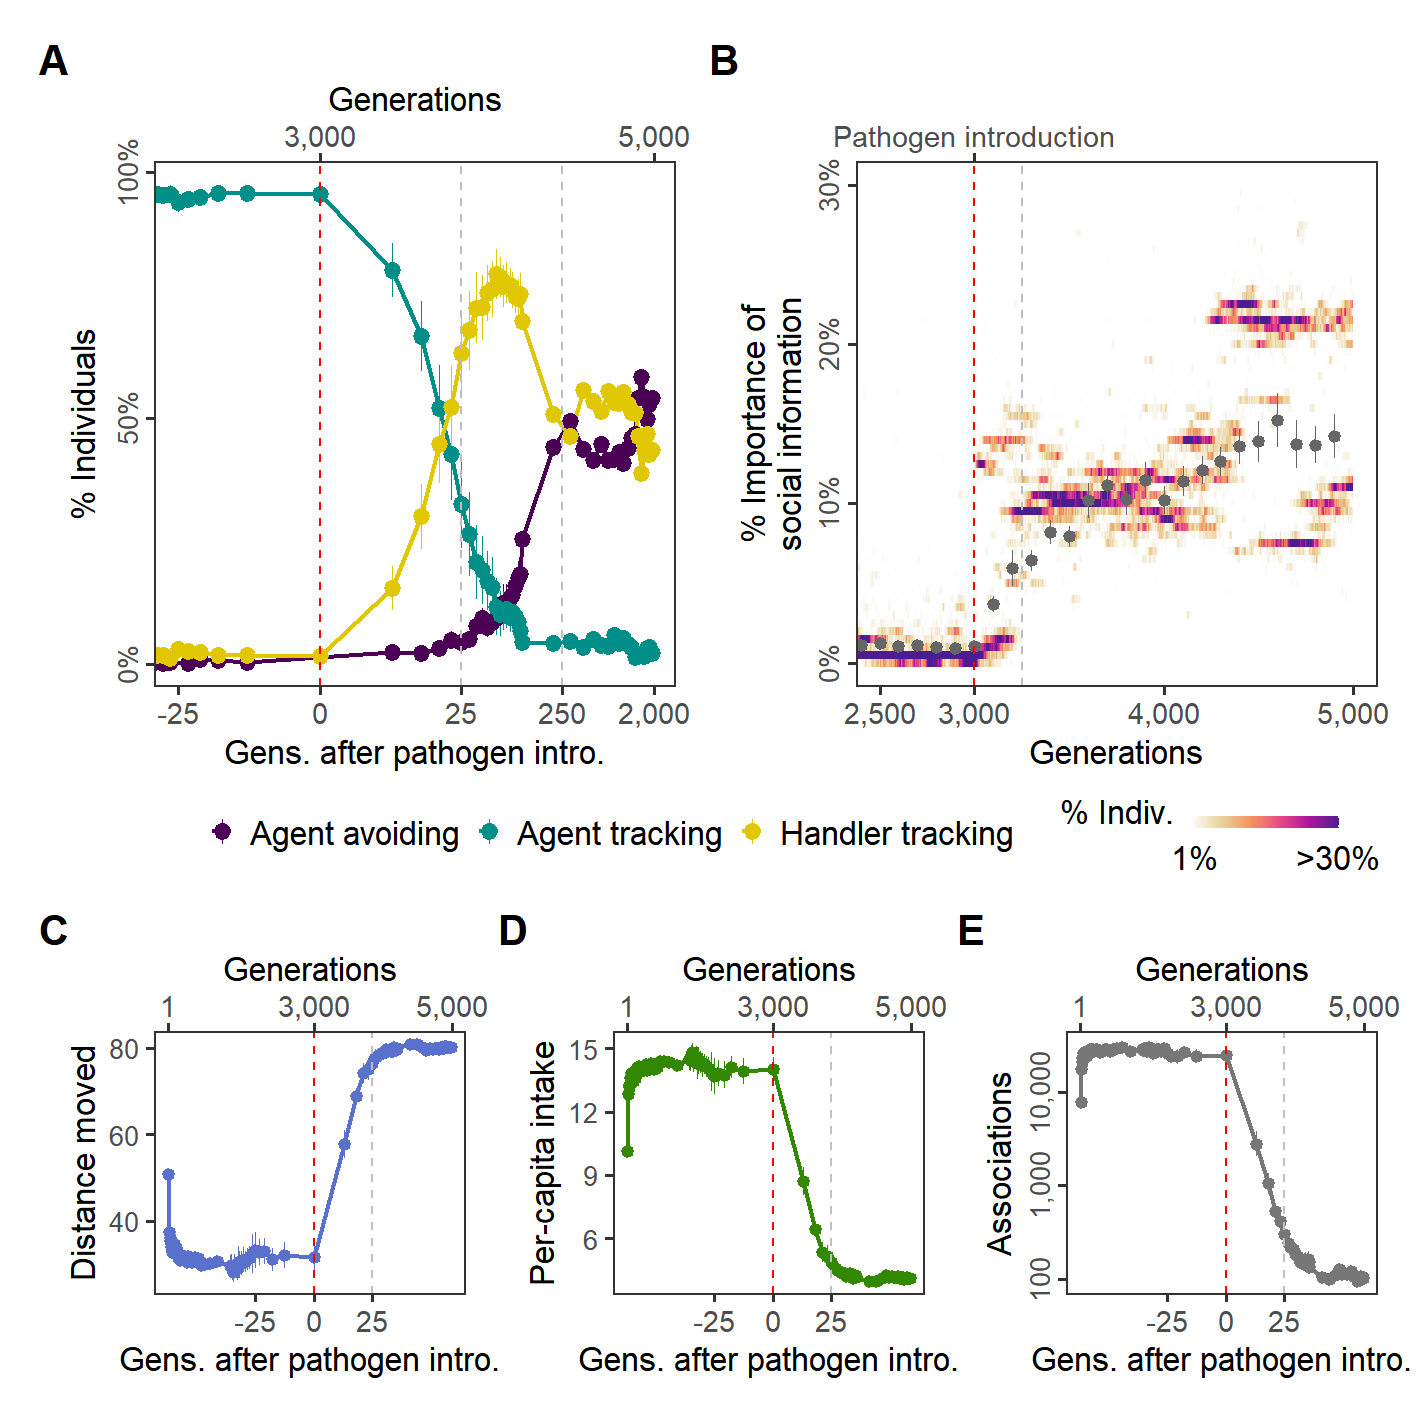
\includegraphics[width=0.7\linewidth]{figures/pathomove/fig_eco_evo_general.png}
    \caption{
        \textbf{Pathogen introduction leads to rapid evolutionary changes in social information use, with cascading effects on population ecological outcomes.}
        \textbf{(A)} Before pathogen introduction in the default scenario (R = 2, $\delta E$ = 0.25), populations rapidly evolve a social movement strategy that tracks all other individuals (`agent tracking'; $G \leq$ 3,000) --- however, their overall movement strategy is primarily guided by the presence of food items \textbf{(B)}.
        Pathogen introduction leads to the rapid replacement, within 25 generations, of agent tracking with `handler tracking' (preference for successful foragers; 3,000 $< G <$ 3,025). 
        Within 250 generations, `agent avoidance' (avoidance of both successful and unsuccessful foragers; $G >$ 3,250) also becomes common, stably co-existing with the handler tracking strategy in an eco-evolutionary equilibrium.
        \textbf{(B)} After pathogen introduction ($G >$ 3,000), the importance of social cues (the presence of other individuals; the sum of the absolute, normalised preferences $sH, sN$) increases substantially on average (grey points).
        Additionally, there is significant variation in the importance of social cues to individuals (shaded regions), which is not captured by the mean or standard error.
        At G = 4,500, for example, social information comprises $\approx$ 10\% of some individuals' movement strategies, but some individuals have evolved a stronger weight for social cues ($>$ 20\%).
        The rapid change in social movement strategies following pathogen introduction has cascading effects on ecological outcomes.
        Individuals, which have evolved strong aversions to at least some kinds of foragers (depending on their strategy), \textbf{(C)} move more on average, \textbf{(D)} have only 25\% of the pre-pathogen average intake, and \textbf{(E)} have 100-fold fewer associations with other individuals.
        All panels show data averaged over 10 replicates, but shaded region in panel B shows only a single replicate for clarity.
    }
    \label{fig_eco_evo_general}
\end{figure}

\subsection*{Disease-dominated Ecological Cascade Due to Evolutionary Shift in Movement Strategies}

The evolutionary shift in social movement strategies causes a drastic change in ecological outcomes (Fig.~\ref{fig_eco_evo_general}C -- E; see \textit{SI Appendix Fig. S3} for other scenarios).
There is a sharp increase in mean distance moved by individuals; while pre-introduction individuals moved 35\% of their lifetimes on average (i.e., 35 timesteps; handling for the remainder), post-introduction, individuals move for 80\% of their lifetimes (i.e., 80 timesteps; Fig.~\ref{fig_eco_evo_general}C).
The handler tracking and agent avoiding strategies lead individuals to move away from groups of individuals \autocite[`dynamic social distancing';][]{pusceddu2021}.
Individuals being most likely to be found near resource clusters, this leads to movement away from productive areas of the landscape.
Consequently, there is a rapid, four-fold drop in mean per-capita intake after pathogen introduction (Fig.~\ref{fig_eco_evo_general}D).
The concurrent, near 100-fold drop in encounters between individuals after pathogen introduction (Fig.~\ref{fig_eco_evo_general}E) suggests that most encounters were likely taking place on or near resource clusters.
The reductions in intake observed are equivalent to those expected from halving landscape productivity (\textit{SI Appendix Fig. S3}).
Our model shows how even a non-fatal pathogen, by influencing the evolution of movement strategies, can have substantial indirect ecological effects --- a disease dominated ecological cascade \autocite{monk2022}.

\subsection*{Co-existence of Social Movement Strategies}

At eco-evolutionary equilibrium (G $>$ 3,500) the relationship between movement and avoiding associations (and further, infection) is mediated by individual differences in how exactly social information is incorporated into movement strategies.
Individuals using the agent avoiding strategy move more than handler tracking ones (Fig.~\ref{fig_social_outcomes}A), about 85\% of their lifetime (default scenario: R = 2; $\delta E$ = 0.25).
At this limit, every step moved allows them to avoid approximately 2 encounters with other individuals.
Handler tracking individuals move much less ($\sim$ 60\% -- 80\%), but are able to avoid approximately 20 encounters with other individuals with every extra step.
These differences may explain why agent avoiding and handler tracking individuals have similar mean infection rates, at $\sim$ 25\% and $\sim$ 33\% respectively (Fig.~\ref{fig_social_outcomes}B).
All other strategies, especially the agent tracking strategy common in pre-introduction populations, are barely able to translate increased movement into fewer associations (Fig.~\ref{fig_social_outcomes}A).
These strategies have a wide range of infection rates (Fig.~\ref{fig_social_outcomes}B), potentially because they are very rare --- these likely represent mutants that do not give rise to persistent lineages.

\begin{figure}[!h]
    \centering
    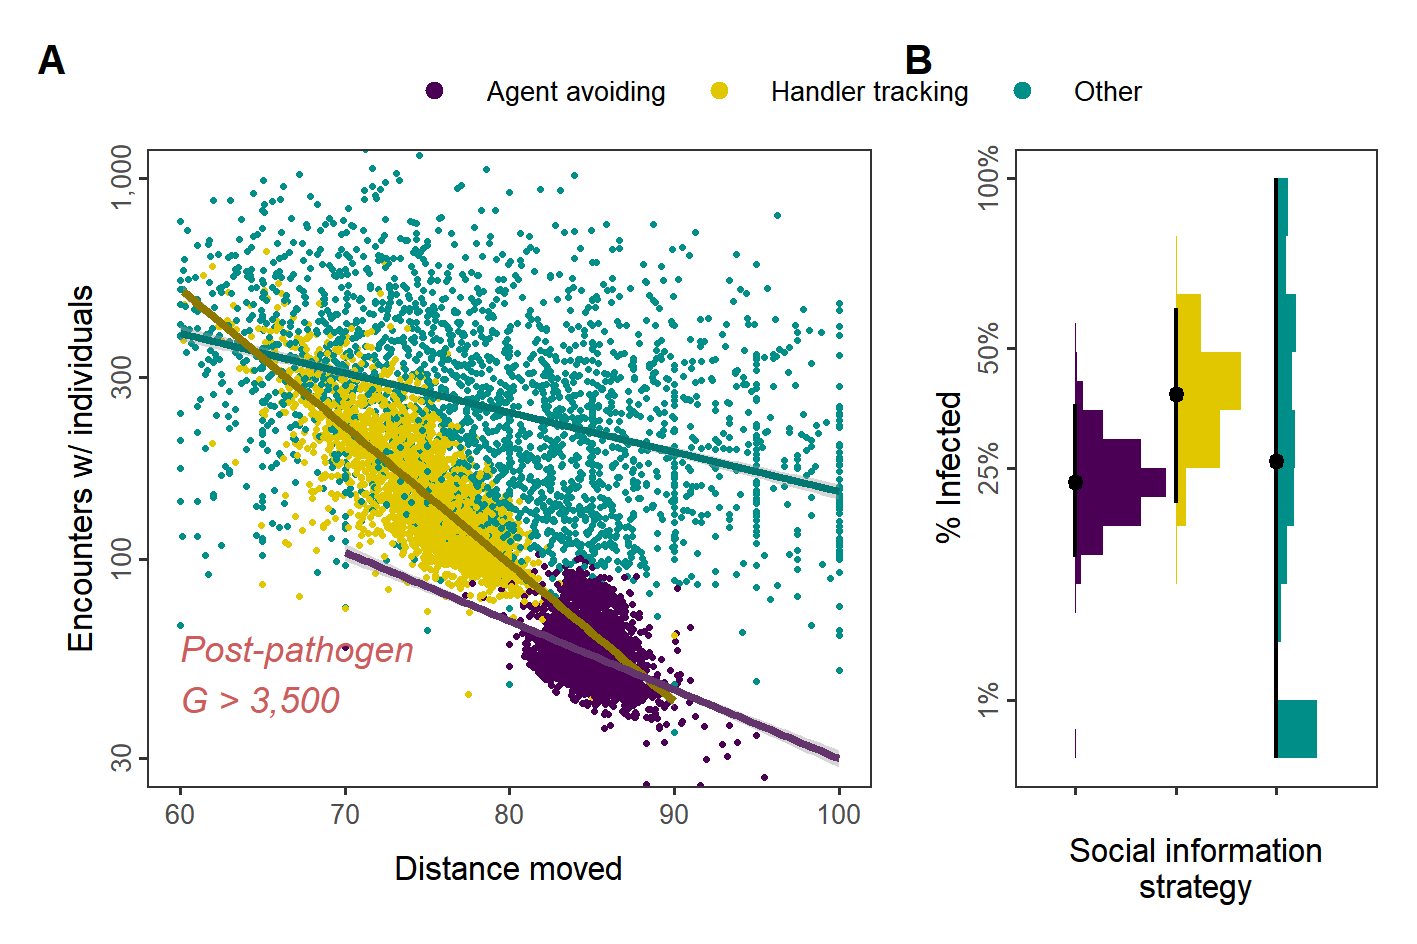
\includegraphics[width=0.7\linewidth]{figures/pathomove/fig_social_outcomes.png}
    \caption{
        \textbf{Social movement strategies trade movement for associations through dynamic social distancing, leading to differences in infection rates.}
        In post-introduction populations at eco-evolutionary equilibrium (G $>$ 3,500), \textbf{(A)} both agent avoiding and handler tracking individuals can reduce encounters with other individuals by moving to avoid other foragers (dynamic social distancing).
        Handler tracking individuals have many more encounters than agent avoiding individuals, but surprisingly, are better able to reduce encounters through increased movement.
        Individuals using other strategies (mostly agent tracking) have a wider range of movement distances, but cannot efficiently avoid other foragers by moving more.
        \textbf{(B)} Avoiding all other foragers leads to marginally lower infection rates than tracking successful foragers (and avoiding unsuccessful ones; handler tracking).
        Surprisingly, rare pre-introduction strategies such as following any nearby individuals (agent tracking) may also have low infection rates, potentially due to their rarity.
        Panel A shows linear model fits with a log scale Y-axis; panel B shows infection rates; all data represent generation- and replicate-specific means (G $>$ 3,500; R = 2, $\delta E$ = 0.25).
    }\label{fig_social_outcomes}
\end{figure}

\subsection*{Reorganisation of Spatial-social Structure}

Following pathogen introduction, the mixture of individual-level movement strategies elicits a substantial re-organisation of emergent spatial and social structure at the population level.
Pre-introduction populations are strongly clustered in space (Fig.~\ref{fig_networks_disease}A), due to movement strategies that favour following most other foragers.
This spatial proximity means that most individuals encounter each other at least once, leading to numerous unique partners (the `degree') for each forager (Fig.~\ref{fig_networks_disease} inset 1: \emph{blue}).
In contrast, the spread-out networks in pathogen-risk adapted populations suggest that most foragers move substantially from their initial locations over their lifetime, associating only ephemerally with foragers from all over the landscape (Fig.~\ref{fig_networks_disease}B).
This reflects movement strategies which lead to near-perpetual movement to avoid associations; a sort of dynamic social distancing seen in real animal societies under risk of pathogen spread \autocite{weinstein2018,stroeymeyt2018,pusceddu2021,stockmaier2021}.
This dispersed population structure means that most pathogen-risk adapted foragers encounter fewer than 10\% of the population over their lifetime (Fig.~\ref{fig_networks_disease} inset 1: \emph{red}).

\begin{figure*}[!h]
    \centering
    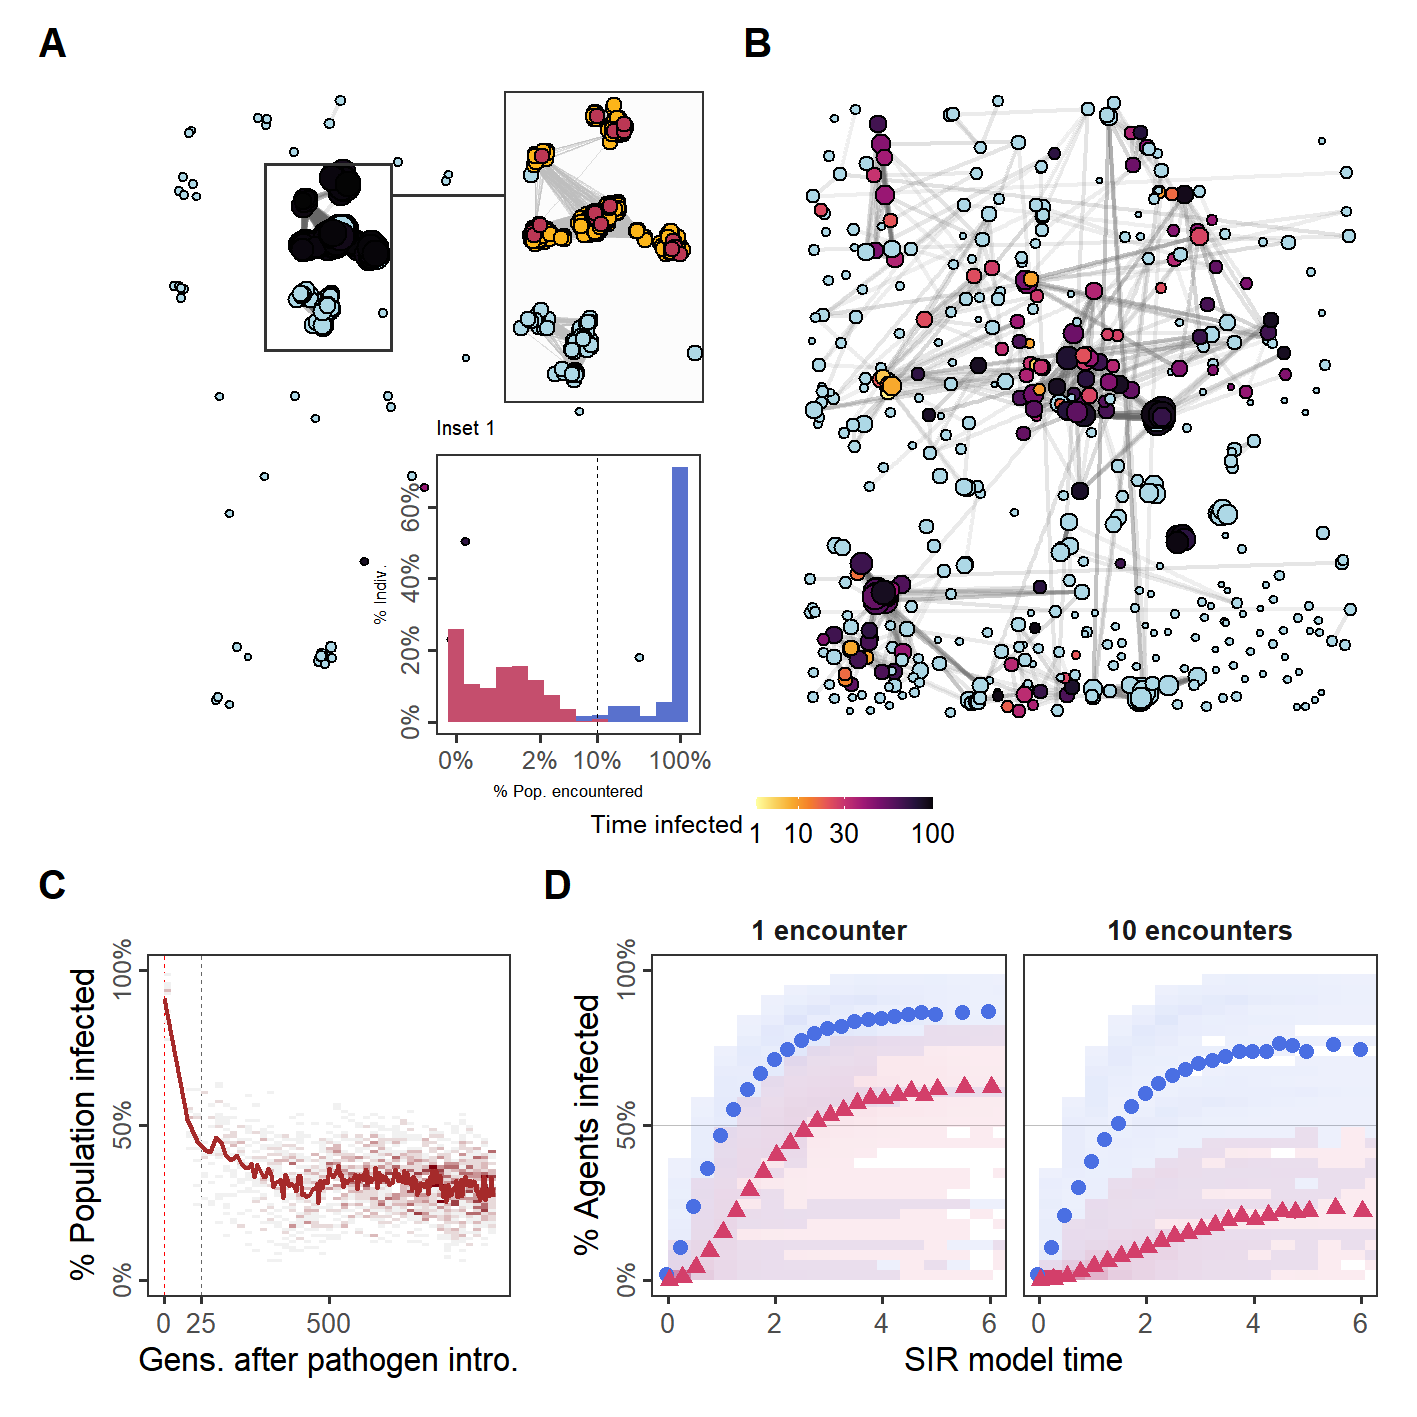
\includegraphics[width=0.9\linewidth]{figures/pathomove/fig_networks_disease.png}
    % width=8.7cm
    \caption{
        \textbf{Reduced spatial-social clustering and disease transmission in populations adapted to the presence of an infectious pathogen.}
        pathogen-risk naive populations (\textbf{A}; G = 3,000) are much more spatially clustered than pathogen-risk adapted populations (\textbf{B}; G = 3,500), and are thus rapidly infected (red: primary infections; yellow: secondary infections; blue: never infected).
        Pre-introduction individuals encounter many more unique neighbours (\textbf{inset 1}, blue) than pathogen-risk adapted individuals (\textbf{inset 1}; red). 
        Dashed grey line represents 10\% of individuals encountered (N = 50).
        Main panels show social networks from a single replicate of the default scenario (R = 2, $\delta E$ = 0.25), insets show 10 replicates. Nodes represent individuals positioned at their final location. Connections represent pairwise encounters, and node size represents encounters (larger = more encounters). Darker node colours indicate longer infection (light blue = no infection). 
        \textbf{(C)} In the first generations following pathogen introduction, nearly every single individual in the population is infected. However, within 25 generations, tracking the evolutionary shift towards movement strategies that avoid some or all other individuals, only about 50\% of individuals are ever infected; this drops to a stable 30\% within 500 generations after pathogen introduction.
        \textbf{(D)} The progression of two hypothetical diseases, requiring a single encounter, or 10 encounters for a potential transmission, on emergent social networks. 
        The transmission of both diseases is reduced in populations with disease-adapted movement strategies (pre-introduction: G = 3,000, blue circles; post-introduction: G = 3,500, red triangles). Subfigures in panel D show means of 25 SIR model replicates (transmission rate $\beta$ = 5.0, recovery rate $\gamma$ = 1.0), run on emergent social network; both panels represent 10 simulation replicates the default scenario.
    }\label{fig_networks_disease}
\end{figure*}

\subsection*{Pathogen-risk adapted Movement Strategies Make Animal Societies More Resilient to the Spread of Disease}

Nearly every individual in the generations just after pathogen introduction was infected.
However, tracking the evolutionary change in movement strategies, the number of infected individuals fell to just about 50\% within 25 generations (Fig.~\ref{fig_networks_disease}C).
To examine potential pathogen spread in pre-introduction populations, we ran a simple epidemiological model on the social networks emerging from individuals' movements before and after pathogen introduction (pre-introduction: G = 3,000; post-introduction: G = 3,500).
We modelled two diseases, \textit{(i)} first, a disease requiring one encounter,and \textit{(ii)} second, a disease requiring ten encounters between individuals for a potential transmission event (transmission rate $\beta$ = 5.0, recovery rate $\gamma$ = 1.0).

Both the single encounter and multiple encounter diseases would infect 75\% -- 80\% of individuals when spreading through the networks of pre-introduction populations (Fig.~\ref{fig_networks_disease}D).
Pathogen-risk adapted populations' social networks are more resilient to both the single encounter and multiple encounter disease, compared to their pre-introduction, pathogen-risk naive ancestors, as these social networks are sparser and individuals are more weakly connected (Fig.~\ref{fig_networks_disease}D).
Less than 60\% of post-introduction populations were finally infected by the single encounter disease, compared with $>$ 75\% of pre-introduction, pathogen-risk naive ancestors; in pathogen-risk adapted populations, the spread of the multiple encounter disease was even slower (ever infected: $\approx$ 20\%).
% the infection peak in pathogen-adapted networks  was only about half as much as for their pathogen-naive ancestors' networks (25\% \textit{versus} 50\% of individuals).

\begin{figure}[!h]
    \centering
    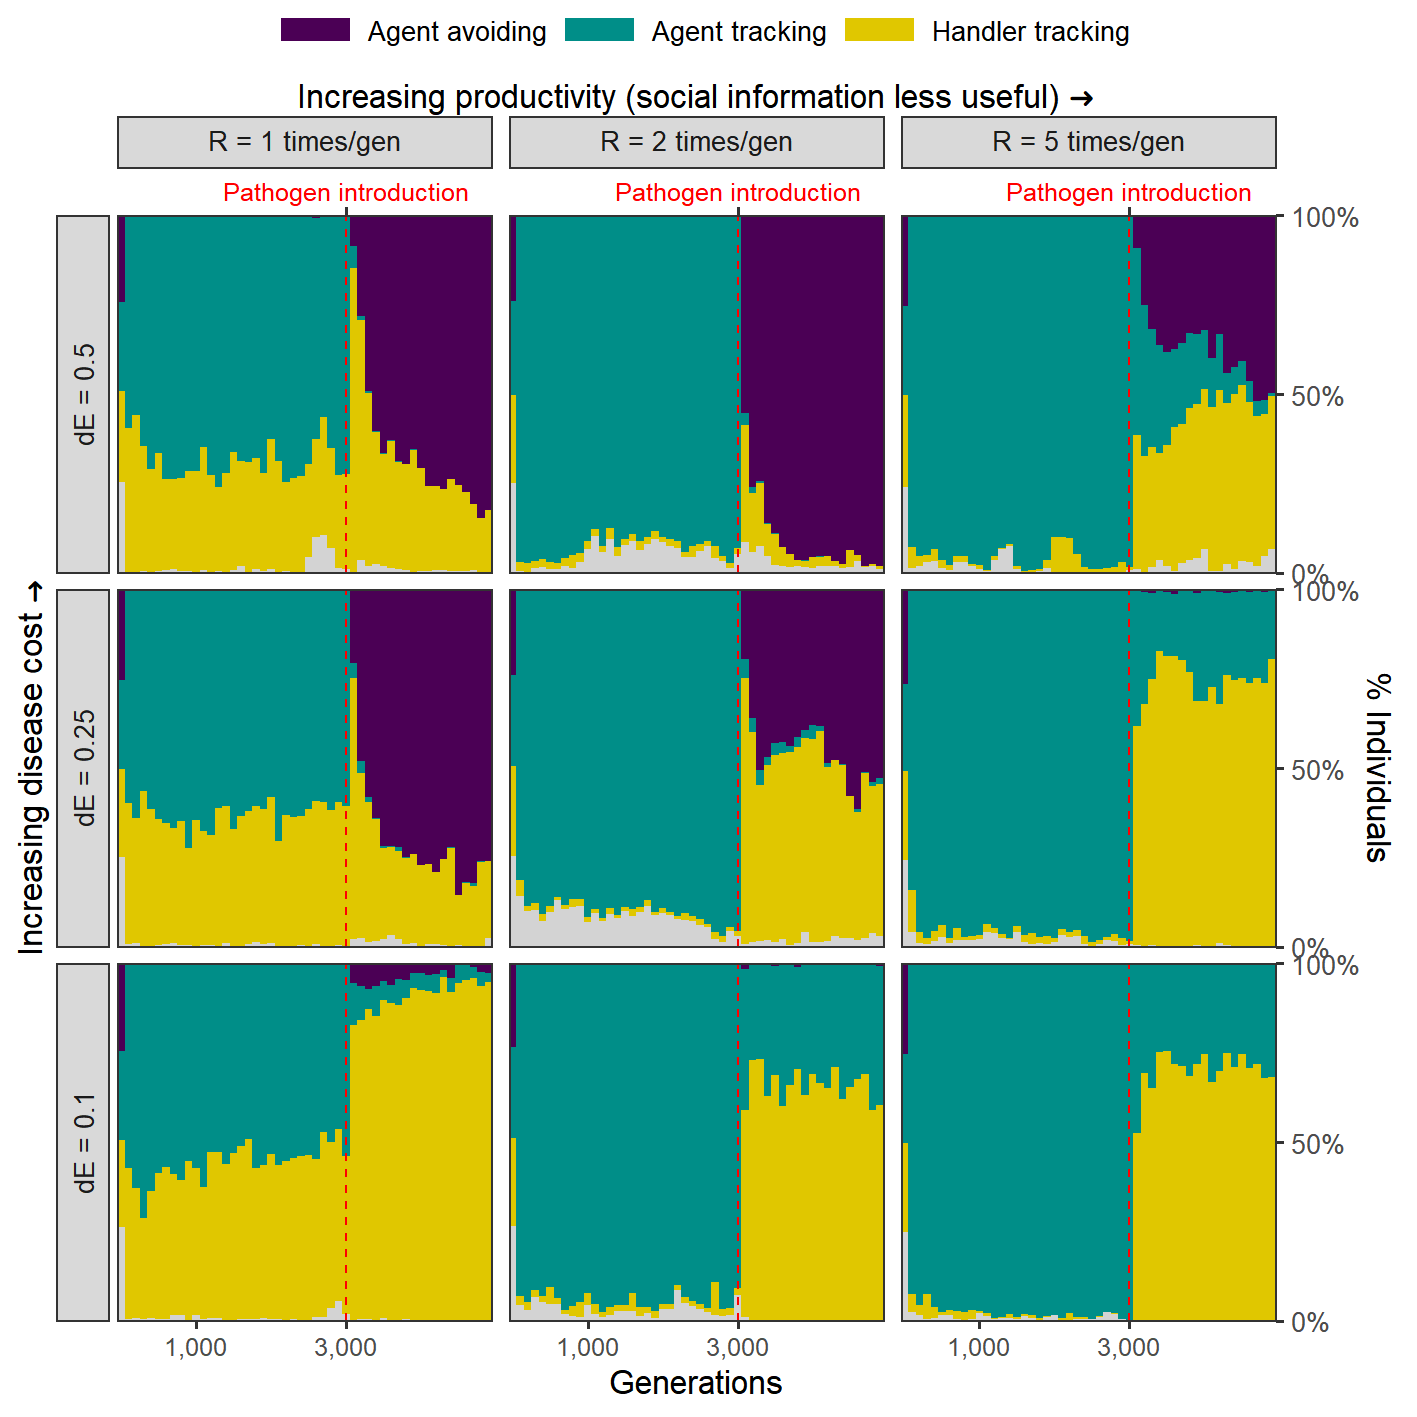
\includegraphics[width=0.9\linewidth]{figures/pathomove/fig_evo_strategy_default.png}
    % width=8.7cm
    \caption{
        \textbf{The balance of infection cost and the usefulness of social information together shape the rapid evolutionary change in movement strategies triggered by pathogen introduction.}
        Pre-introduction (G = 3,000; dashed line) populations contain a mix of individuals that either track all foragers (agent tracking), or only successful foragers (handler tracking).
        Handler tracking is more common on low-productivity landscapes (R = 1), where social information is more useful to find patchily distributed resources.
        After pathogen introduction, handler tracking rapidly becomes the most common strategy when the apparent usefulness of social information is greater than the cost of infection.
        This occurs both when productivity is low (R = 1) and infection costs are low ($\delta E$ = 0.1), but also when productivity is high (R = 5) with intermediate infection costs ($\delta E$ = 0.25).
        When the cost of infection outweighs the apparent usefulness of social information, the agent avoidance (avoiding both successful and unsuccessful foragers) emerges and rapidly becomes a common strategy ($\delta E$ = 0.5; $\delta E$ = 0.25, R = 1).
        In scenarios of high landscape productivity combined with low infection costs (e.g. R = 5, $\delta E$ = 0.1), the agent tracking strategy persists in a large proportion after pathogen introduction, as these individuals can balance disease costs with intake alone.
        All panels show mean frequencies over 10 replicate simulations in 100 generation bins; frequencies are stacked.
        Grey areas show the relatively uncommon `non-handler' tracking strategy.
    }\label{fig_evo_strategy}
\end{figure}

\subsection*{Usefulness of Social Information and Infection Cost Influence Evolution of Social Movement Strategies}

We further explored the effect of two ecological parameters, landscape productivity ($R \in $ 1, 2, 5) and infection cost per timestep ($\delta E \in$ 0.1, 0.25, 0.5) on simulation outcomes.
Before pathogen introduction, landscape productivity alone determines the value of social information, and thus which social movement strategies evolve (Fig.~\ref{fig_evo_strategy}).
On low-productivity landscapes (R = 1), social information is valuable as direct resource cues are scarce; here, the handler-tracking strategy persists.
On high-productivity landscapes ($R \in$ 2, 5), social information is less valuable as individuals can directly detect food items more often; here, the agent tracking strategy is most common.
Across parameter combinations, the introduction of the infectious pathogen leads to a rapid evolutionary shift in social movement strategies.
The benefits of social information, and infection cost jointly determine how pathogen introduction alters the mix of social movement strategies, but populations generally shift away from indiscriminate agent tracking, as that strategy is associated with higher infection risk (see Fig.~\ref{fig_networks_disease}A).

When the benefit of social information is equivalent to the cost of infection, the handler tracking strategy is common (R = 1, $\delta E$ = 0.1; R = 5, $\delta E$ = 0.25).
When apparent social information benefits are lower than infection costs (e.g. $\delta E$ = 0.5), the agent avoiding strategy is common.
The effect of landscape productivity in obviating a sensitivity to social information cues (especially, conspecific status) is also eroded by pathogen introduction.
On high-productivity landscapes where individuals were indiscriminately social, ($R \in$ 2, 5, $\delta E$ = 0.1), the handler tracking strategy becomes common, as individuals prioritise higher-quality social information (handlers, which indicate a resource cluster).
However, high landscape productivity can also compensate for the cost of infection, as evidenced by the agent tracking strategy remaining prevalent: this is only possible if these individuals can consume sufficient resources to overcome disease costs.

\section*{Contextualising the Outcomes of the Pathomove Model}

Our general model captures important features of infectious pathogen (or parasite) transmission among host animals in a (foraging) context that is relevant to most species.
The combination of ecological, evolutionary, and epidemiological dynamics in a spatial setting is unprecedented for movement-disease models, and 
% Our approach shows how evolution can be incorporated into mechanistic movement-disease models, and how this approach 
extends current understanding of animal spatial and social ecology \autocite{albery2021,webber2018,webber2022,romano2020,romano2021,kurvers2014}.
Presently, most movement-disease models are non-evolutionary \autocite{white2018,white2017,scherer2020,lunn2021}, presumably because evolution is expected to be too slow to impact epidemiological-ecological outcomes \autocite{monk2022}.
We demonstrate the pitfalls of this assumption: evolutionary transitions in sociality occur over fewer generations than required for the development of key aspects of animal ecology, such as migration routes \autocite{jesmer2018,cantor2021}.
We also demonstrate the tension inherent to sociality under the risk of an infectious pathogen, in an explicitly spatial context.
% We show how populations, initially evolved to find patchily distributed food using social information, rapidly evolve to become more sensitive to potential infection risk and eschew (some) social encounters, when an infectious pathogen is introduced.
Our work shows how qualitatively and quantitatively different social movement strategies --- making different trade-offs between social information and infection risk --- can co-exist in a single population \autocite{wolf2012,webber2018,gartland2021,webber2022}.

\subsection*{Social Information Use and Pathogen Introduction}

<<<<<<< HEAD
Prior to pathogen introduction, the value of social information influenced which social movement strategies were evolved. 
Individuals initialised (`born') near their parent's final location may benefit from `ecological inheritance' \autocite{badyaev2009} of their parent's favourable position near resource clusters (see \textit{SI Appendix Fig. S2, S4}).
Avoiding potential competitors (and kin) thus correlates with avoiding profitable areas, and this leads to the persistence of the indiscriminately social agent tracking strategy, despite the evident costs of exploitation competition.
In an alternative implementation with large-scale natal dispersal, handler tracking is the commonest strategy prior to pathogen introduction (see \textit{SI Appendix}).
Following pathogen introduction, the agent tracking strategy of our default scenario allows the disease to spread very easily among entire lineages of social individuals (see Fig.~\ref{fig_networks_disease}A) \autocite{kurvers2014}.
This neatly demonstrates why the risk of infection or parasitism could be among the mechanisms underlying density dependence in natal dispersal decisions \autocite{travis1999}.

Following pathogen introduction, the evolutionary shift in social movement strategies is much more rapid than the timescales usually associated with the evolution of complex traits such as sociality (about 25 generations).
Avoiding potentially infectious individuals is a key component of navigating the `landscape of disgust' \autocite{weinstein2018}.
Our results show that sensitivity to cues of high pathogen transmission risk can rapidly evolve following the introduction of a novel pathogen, with a complete replacement of the hitherto dominant social strategy.
The emergence of qualitative individual variation in social movement strategies, and especially the trade-off between movement, associations, and infection risk also demonstrates the evolution of `sociability as a personality trait' \autocite[][]{gartland2021}.

We also find substantial individual variation in the quantitative importance of social cues overall, which is a key component of the evolution of large-scale collective behaviours, such as migration \autocite{guttal2010}.
Our work suggests how, by leading to the necessary diversity in social movement strategies, a novel pathogen may actually lay the groundwork for the evolution of more complex collective behaviour.
Nonetheless, the rapid decreases in social interactions should primarily prompt concern that the evolutionary consequences of pathogen introduction could slow the transmission of, and erode, animal culture \autocite{cantor2021} --- including foraging \autocite{klump2021} and migration behaviours \autocite{jesmer2018,guttal2010}.
Pathogens themselves typically have shorter generation times than their hosts, and may also evolve rapidly in response to changes in host sociality \autocite{ashby2022}.
Although not examined here, a mixture of social strategies could allow for the maintenance of a corresponding diversity in pathogen strategies as well \autocite{ashby2022,prado2009}.
=======
We expected that prior to pathogen introduction, exploitation competition should promote the use of high-quality social information, and the avoidance of potential competitors \citep[handler tracking;][]{gupte2021a}.
We found that the usefulness of social information affected this outcome quite strongly, as handler tracking was most common on low-productivity landscapes ($R$ = 1), where social information is crucial to finding resources (see \textit{Model and Analysis}).
Our current model's landscape clusters are more sparsely and irregularly distributed than in our previous work \citep{gupte2021a}, and individuals are initialised near their parent's final location (see \textit{Supplementary Information}).
This leads to `ecological inheritance' whereby successful individuals on or near resource clusters pass their favourable positions on to their offspring \citep{badyaev2009}.
Avoiding potential competitors thus correlates with avoiding profitable areas.
This leads to the persistence of the indiscriminately social agent tracking strategy, despite the evident costs of exploitation competition (see \textit{Supplementary Information} for an alternative implementation).
We found an unexpectedly rapid evolutionary shift, within 25 generations, in individual movement strategies following pathogen introduction.
This is much more rapid than the timescales usually associated with the evolution of complex traits such as sociality.
This change actually occurs over fewer generations than over which key aspects of animal culture and ecology, such as migration routes, are established through social learning \citep{jesmer2018,cantor2021}.
Current and expected cross-species transmissions of novel pathogens \citep{carlson2022a,pusceddu2021} should thus prompt concern that the evolutionary consequences of pathogen introduction could slow the transmission of, and erode, animal culture \citep{cantor2021}.

Avoiding potentially infectious individuals is a key component of navigating the `landscape of disgust' \citep{weinstein2018}.
To navigate this landscape effectively, animals must first be sensitive, or become more sensitive, to cues of high transmission risk.
Our results show that such sensitivity can rapidly evolve following the introduction of a novel pathogen, leading to strong qualitative changes in movement strategies within 100 generations.
Furthermore, on average, individuals' sensitivity to social movement cues actually increases after pathogen introduction.
However, there was substantial between-individual variation in the importance of social cues overall, even after a specific movement strategy had become dominant.
A mix of individuals with different sensitivities to social cues, relative to resource cues, is key to the evolution of large-scale collective behaviours, such as migration \citep{guttal2010}.
Our work suggests how in the long term (about 500 generations), by leading to the necessary diversity in social movement strategies, a novel pathogen may actually lay the groundwork for the evolution of more complex collective behaviour.
The emergence of individual variation in social movement strategies, and especially the trade-off between movement, associations, and infection risk also suggests a clear mechanism by which sociality could evolve as a personality trait \citep[][]{gartland2021}.
>>>>>>> 8d43b47ddc128b0830158c7f25ae286fb9050a49

\subsection*{Ecological Causes and Consequences of Social Movement Strategies}

In our model, landscape productivity (R), is a proxy for the usefulness of sociality overall, as social information is less useful when direct resource cues are abundant (high R).
Social information benefits in disease models often have no mechanistic relationship with the subject of the information (e.g. food or predators) \autocite{ashby2022}. 
In contrast, social information benefits in our model are emergent outcomes of animal movement and foraging behaviour. 
Our predictions may help explain intra- and inter-specific diversity in social systems across gradients of infection risk and the usefulness of social information \autocite{altizer2003,sah2018}, and studies tracking social movements and potential for disease spread could form initial tests of our basic predictions \autocite{wilber2022}.
While our individuals do not die, the evolved pathogen-risk adapted, dynamic social distancing strategies \autocite{stockmaier2021} lead to a significant worsening (equivalent to a halving) of individuals' intake.
In real systems, this could increase populations' susceptibility to extreme climate change related mortality events \autocite{fey2015}.

More positively, animals may be able to adapt relatively quickly to the spillover and eventual persistence of infectious pathogens, even when they cannot specifically detect and avoid infected individuals \autocite{altizer2003,stroeymeyt2018,stockmaier2021,pusceddu2021}.
While the most noticeable effect of pathogen outbreaks is mass mortality \autocite{fey2015}, even quite serious pathogens --- Sarcoptic mange \autocite{almberg2015}, foot-and-mouth disease \autocite{jolles2021,bastos2000,vosloo2009}, SARS-CoV-2 \autocite{chandler2021,kuchipudi2022}, and avian influenza \autocite{globconsorth5n82016,wille2022} among others --- appear to spread at sub-lethal levels for many years between lethal outbreaks.
Our model shows how disease-dominated ecological cascades \autocite{monk2022} 
% --- individuals have less intake, exerting less top-down pressure on their resource --- 
could occur even without mortality effects, due to evolutionary shifts in sociality alone.
% In the \textit{SI Appendix}, we show that such a cascade occurs even when the infection costs are modelled quite differently, being considered to be a fraction of daily intake.
The altered ecological state \autocite[here, less resource consumption, as in][]{monk2022} may be maintained long after --- and indeed because --- a population has adapted to be less social in the presence of a pathogen.
Our work suggests that decreased sociality resulting from adaptation to a novel pathogen could slow the transmission of future novel pathogens. 
While decreased sociality could also reduce the prevalence of previously endemic pathogens adapted to a more social host, it may also degrade `social immunity' through reduced sharing of beneficial commensal microbes, or of low, immunising doses of pathogens \autocite{ezenwa2016,almberg2015}.

\subsection*{Feedbacks with Pathogen Chracteristics}

Our model results are contingent upon sustained introduction of the pathogen (or its novel strains) to host populations.
More sporadic introductions (once every few generations) apparently do not cause evolutionary shifts in social movement (\textit{SI Appendix}).
Yet repeated pathogen and parasite introductions among susceptible populations appear to be quite common \autocite{levi2012,jolles2021,vosloo2009,bastos2000,scherer2020,globconsorth5n82016,wille2022}.
Such introductions are often detected only among easily observed groups such as birds \autocite{wille2022}, or after evident mass mortality events \autocite{fey2015,fereidouni2019}.
Seasonal host-pathogen dynamics could and do keep pathogens circulating in reservoir hosts, with regular pulses in primary infections similar to our model (e.g. due to new calves in African buffalo hosting foot-and-mouth disease: \cite{jolles2021}, or winter peaks in mange among wolves: \cite{almberg2015}).
Existing host-pathogen dynamics, and potential pathogen range expansions, could thus provide more frequent opportunities for novel transmissions to overlapping species than previously guessed.
Our model shows how this provides a powerful selective force in favour of detecting and avoiding infection risk cues \autocite{weinstein2018}.

Pathogens also typically have much shorter generation times than their hosts.
Analytical models expect pathogen attributes to rapidly co-evolve to match host population attributes (e.g. sociality and immune resistance) \citep[][]{bonds2005,prado2009,ashby2022}.
Such models treat pathogens --- just as they do host animals --- in relatively simple, non-mechanistic ways.
Pathogens are primarily expected to evolve to a virulence that promotes between-host transmission \citep{bonds2005}.
Our mechanistic model does not explicitly consider host-pathogen co-evolutionary dynamics, as this complexity was beyond the scope of our general, conceptual model.
Adding pathogen evolutionary dynamics to a mechanistic individual-based model would require careful consideration of \textit{(i)} the costs the pathogen imposes on its hosts, and \textit{(ii)} how it transmits between hosts, both within and between generations.
We expect that multiple pathogen strategies could coexist in a host population that itself has multiple social movement strategies.

\subsection*{Towards Hypothesis-testing and Predictive Modelling}

In order to be widely applicable to diverse novel host-pathogen introduction scenarios, our model is necessarily quite general.
A wide diversity of pathogens and their dynamics remains to be accurately represented in individual-based models \autocite{white2017,white2018,scherer2020,lunn2021}. 
Our framework can be expanded and specifically tailored to real-world situations in which populations are repeatedly exposed to novel pathogens (or strains) \autocite{scherer2020,wille2022,bastos2000,jolles2021,chandler2021,kuchipudi2022}.
Such detailed implementations could include aspects of the pathogen life-cycle \autocite{white2018a,white2017}, account for sociality as a counter to infection costs \autocite{ezenwa2016,almberg2015}, or model host-pathogen sociality-virulence co-evolution \autocite{ashby2022,prado2009,bonds2005}.
We generate consistent predictions of marked and swift evolutionary shifts in social movement strategies that could plausibly be tested over the timescales of some long-term animal tracking studies \citep{wilber2022}.

Importantly, our social information-based movement strategies are made up of continuous values that place individuals on a two-dimensional trait space of relative preferences (or aversions) for successful and unsuccessful foragers (see \textit{Model and Analysis}; \cite{bastille-rousseau2019}).
Such social movement strategies could already be revealed for free-living animals using newer step-selection approaches \citep{avgar2016}, combined with the simultaneous, high-throughput tracking of many hundreds of animals in an area \citep{nathan2022}.
Future work would ideally combine wildlife monitoring and movement tracking across gradients of pathogen prevalence, to detect novel cross-species spillovers \autocite{chandler2021,kuchipudi2022} and study the spatial and epidemiological consequently of animal movement strategies \autocite{bastille-rousseau2019,wilber2022,monk2022}.
Given that infection patterns can change rapidly in space even in small, well-mixed populations \citep{albery2022}, the systems that could be used to test these phenomena may be widespread and easily available.
Finally, our model shows why it is important to consider evolutionary responses in movement-disease studies, and provides a general framework to further the integration of evolutionary approaches in wildlife spatial epidemiology.

% \subsection*{Data and Code Availability}

% The \textit{Pathomove} simulation model code is available on Zenodo at https://zenodo.org/record/6331816, and on Github at github.com/pratikunterwegs/pathomove.
% A reference dataset with 10 replicates of the parameter combinations presented here is archived on Zenodo at: https://zenodo.org/record/6331757.
% Code to run the simulations and analyse the output is on Zenodo at https://zenodo.org/record/6341440, and on Github at: 
% github.com/pratikunterwegs/patho-move-evol.

% \subsection*{Acknowledgements}
% We thank Jan Kreider for helpful feedback on an early draft of the manuscript;
% and Thijs Janssen for help with the simulation model code.
% We thank the Center for Information Technology of the University of Groningen for providing access to the \textit{Peregrine} high performance computing cluster to run simulations.
% P.R.G was supported by an Adaptive Life Programme grant made possible by the Groningen Institute for Evolutionary Life Sciences (GELIFES).
% J.G. was supported by a grand from the Netherlands Organization for Scientific Research (NWO-ALW; ALWOP.668).
% F.J.W. acknowledges funding from the European Research Council (ERC Advanced Grant No. 789240).

{ \begin{center} \barfont{-.-} \end{center} }

\newpage

\begingroup

\let\clearpage\relax
\let\cleardoublepage\relax
\let\cleardoublepage\relax

{\chapter*{Supplementary Information}}

\section*{Data and Code}

The \textit{Pathomove} simulation model code is available on Zenodo at https://zenodo.org/record/6782640, and on Github at github.com/pratikunterwegs/pathomove.
Code to run the simulations and analyse the output is on Zenodo at https://zenodo.org/record/6782665, and on Github at: 
github.com/pratikunterwegs/patho-move-evol.

\section*{Description of the Pathomove Model}

\begin{figure}[!h]
    \centering
    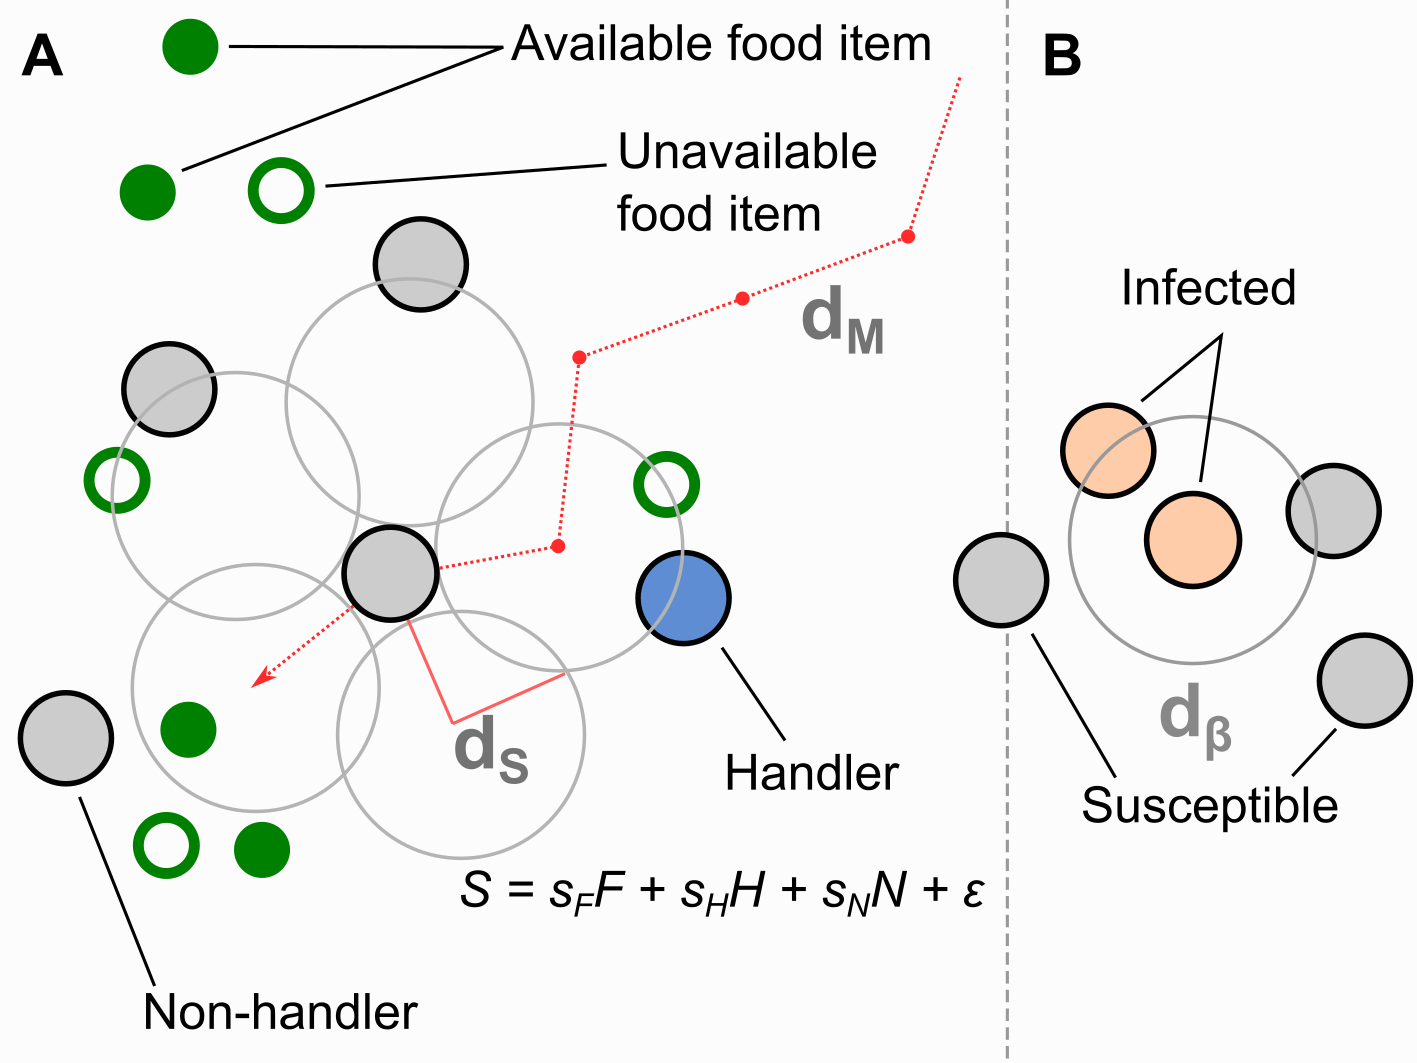
\includegraphics[width=0.9\textwidth]{figures/pathomove/fig_schematic.png}
    \caption{
        \textbf{Model implementation of discrete movement steps in continuous space, with movement steps selected based on inherited preferences for environmental cues.} 
        In our model, \textbf{(A)} individuals search for food items (\textbf{green circles}), which may be immediately available (\textbf{filled green circles}; \emph{F}), or may be available only in the future (\textbf{open green circles}). 
        Individuals can sense only available items, and not unavailable ones. However, given our landscape structure, food items are clustered, making available items a good indicator of where resource clusters are (see next figure). 
        Individuals can also sense other foraging individuals, and can sense whether they have successfully found, and are handling, a food item (handlers; \textbf{blue circles}), or whether they are unsuccessful foragers still searching for food (non-handlers; \textbf{filled grey circles}; \emph{N}). 
        To decide where to move, individuals sample their environment for these three cues (\emph{F, H, N}) at 5 locations around themselves (\textbf{large open grey circles}), and have a sensory range of \(d_S\). 
        When the sensory range is relatively large (default = 1.0 units), there is some small overlap in samples. 
        Individuals assign each potential direction a \emph{suitability}, \(S = s_FF + s_HH + s_NN + \epsilon\), where the coefficients \(s_F, s_H, s_N\) are inherited preferences for environmental cues, and \(\epsilon\) is a small error term that helps break ties between locations. 
        In our implementation, the sensory distance (\(d_S\)) and the movement distance (\(d_M\)) are the same, 1.0 units. 
        \textbf{(B)} Our infectious pathogen is transmitted between infected (\textbf{orange circles}) and susceptible (\textbf{filled grey circles}) individuals, with a probability \(p\) = 0.05, when they are within a distance \(d_\beta\) of each other. 
        In our implementation, \(d_\beta\) is the same as \(d_S, d_M\) = 1.0 units.
    }\label{fig:patho_schematic}
\end{figure}

\begin{figure}
    \centering
    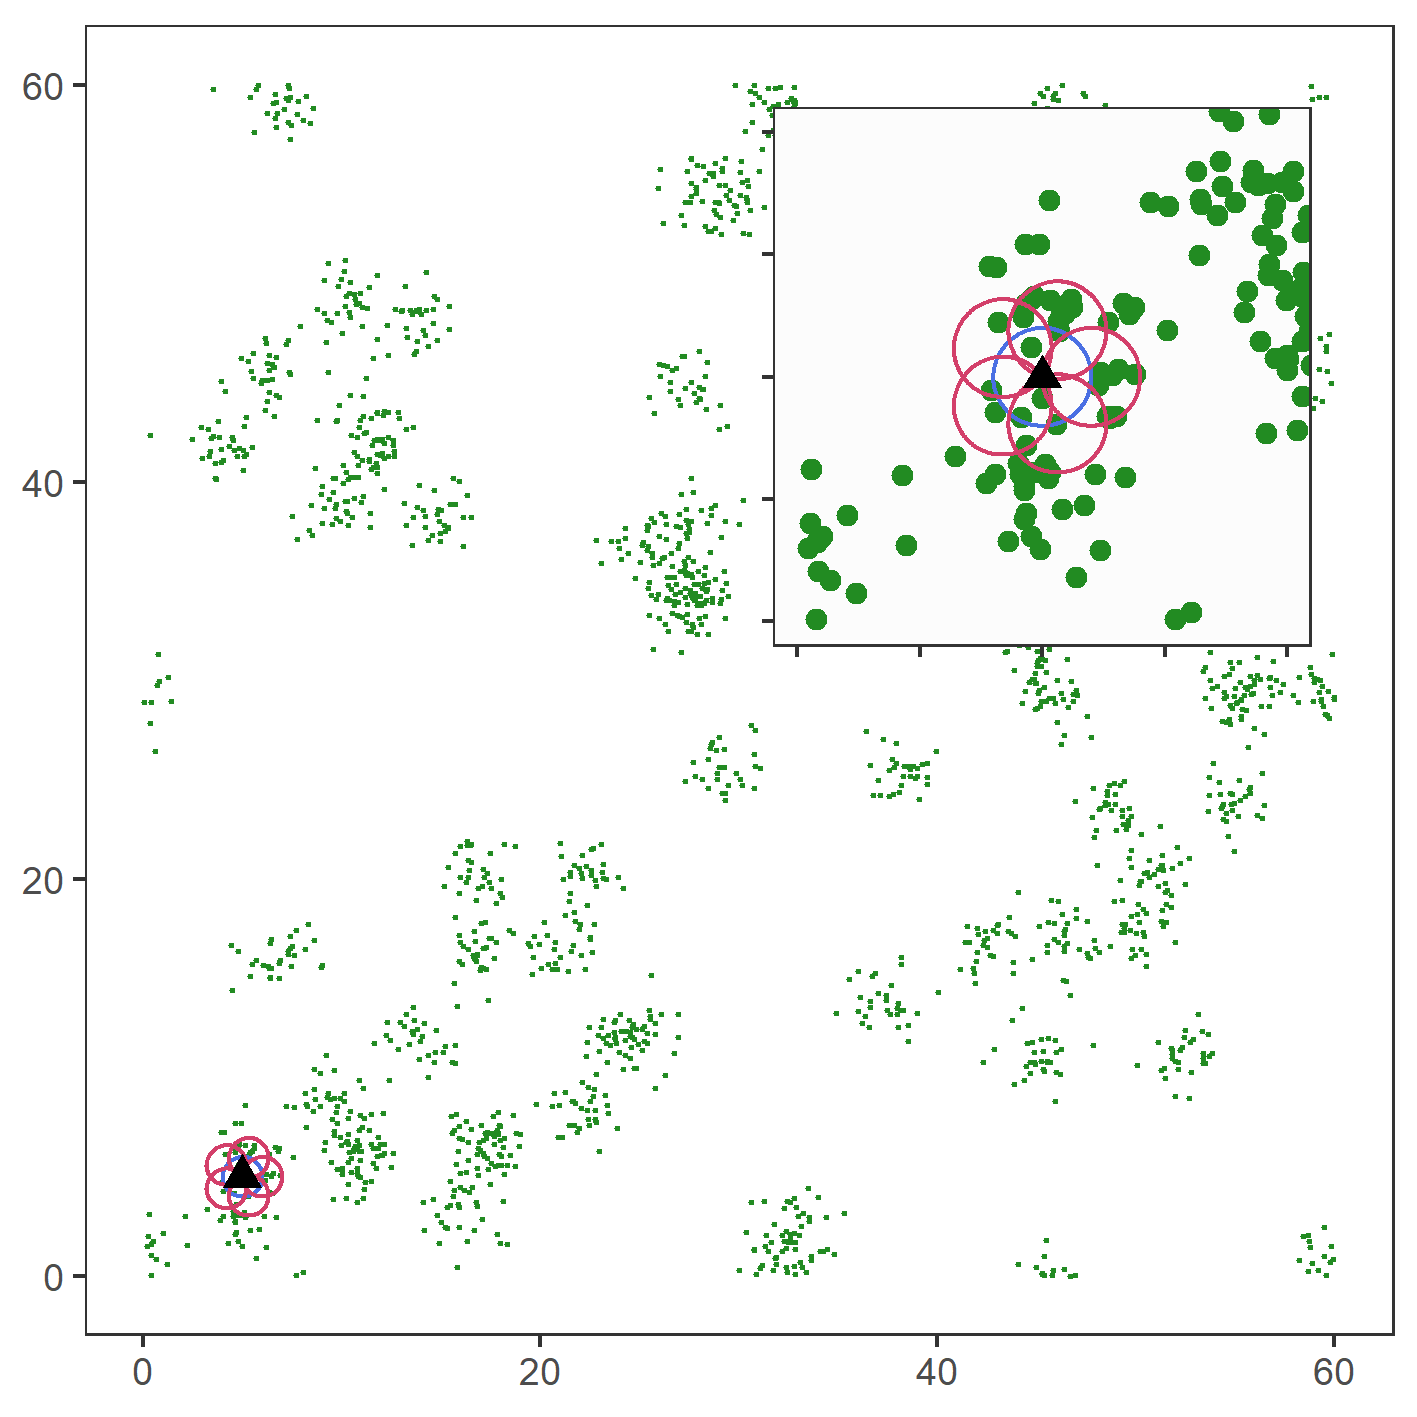
\includegraphics[width=0.7\textwidth]{figures/pathomove/fig_landscape.png}
    \caption{
        \textbf{An example of the resource landscape used in our simulations.} 
        Our simulation's resource landscape consists of 60 randomly distributed clusters of food items (`resource patches'), with 1800 discrete food items divided among the clusters (30 items per cluster). 
        The landscape is a square of 60 units per side, with wrapped boundaries (i.e., a torus). 
        The food item density in our scenarios is 0.5 food items per unit area. 
        Items are distributed around the centre of each cluster, within a standard deviation of 1.0 unit. 
        Items, once consumed by foragers, are unavailable for a fixed number of timesteps (the regeneration time $R$, expressed in terms of the foragers' generation time), after which they regenerate in the same location. 
        While regenerating (i.e., unavailable). While regenerating, items cannot be sensed by foragers. 
        The sensory ranges of individuals (\(d_S\)) are shown for each potential step (\textbf{red circles}, including the current location: \textbf{blue circle}). 
        Food item clustering means that available items, as well as foragers handling a food item (handlers) are good indicators of the location of a resource cluster.
    }\label{fig:patho_landscape}
\end{figure}

\section*{Comparing Ecological Outcomes Across Parameter Combinations}

\begin{figure}
    \centering
    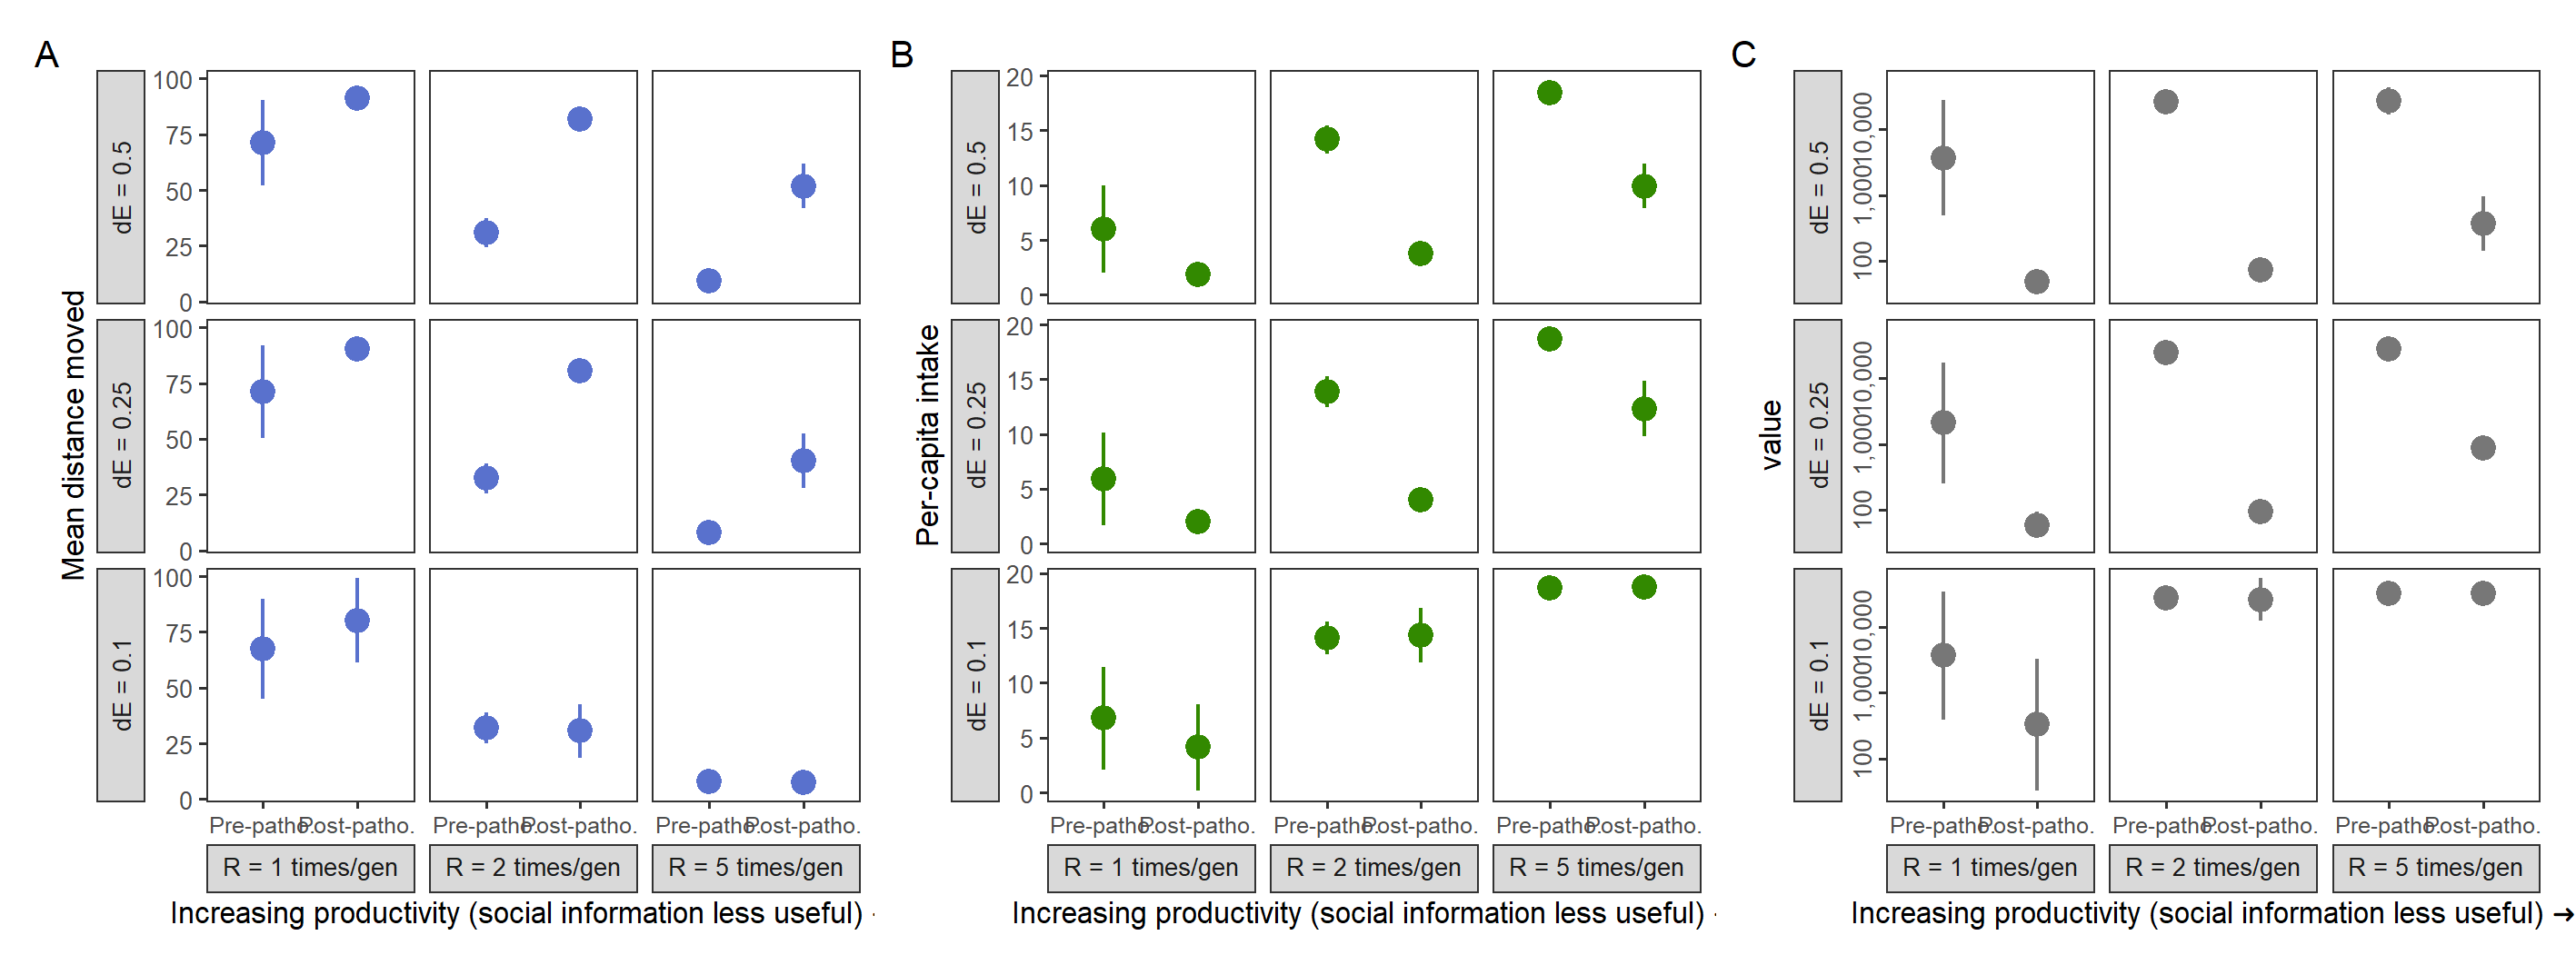
\includegraphics[width=0.95\textwidth]{figures/pathomove/fig_eco_compare_default.png}
    \caption{
        \textbf{Rapid changes in ecological outcomes following pathogen introduction.} 
        The introduction of the infectious pathogen leads to rapid evolutionary changes in movement strategies (see Figures 1 and 5; main text) across most combinations of landscape productivity and infection cost. 
        In all combinations where there is rapid evolutionary shift in social-movement strategies, there is a similar change in the population's ecological outcomes: more movement, less intake, and fewer associations. 
        Only in scenarios where the mix of social-movement strategies does not change (\(R \in\) 2, 5; $\delta~E$ = 0.1), is there broadly no change in population ecological outcomes. 
        Each subplot in each panel shows the mean and standard error of the per-capita values for \textbf{(A)} distance moved, \textbf{(B)} intake, \textbf{(C)} number of associations, or encounters, with other individuals. 
        Means and standard deviations are shown before (G = 3,000) and after (G = 3,500) pathogen introduction; each data point represents 10 replicates of the relevant parameter combination.
    }\label{fig:patho_eco_compare}
\end{figure}

\section*{Effect of Modelling Choices}

Modelling choices can have a substantial effect on the outcomes of simulations with multiple, complex interactions among components \parencite{scherer2020,gupte2021a,netz2021}.
We show the effect of varying implementation on two key aspects of our model: \textit{(1)} where individuals are initialised, or `born', on the landscape (natal dispersal), \textit{(2)} how the infectious pathogen imposes fitness costs.

\subsection*{Global Natal Dispersal of Individuals}

Some models initialise the individuals in each new generation at random locations on the landscape (see e.g. \cite*{gupte2021a}; Chapter~\ref{ch:kleptomove}); this can be called `global' natal dispersal.
This is a reasonable choice when modelling animals during a specific stage of their life cycle, such as after arriving on a wintering or breeding site after migration.
Our default choice, on the other hand, is `local' natal dispersal, where individuals are initialised close to their parent's last position.
This is also defensible, as many organisms do not disperse very far from their ancestors.
When animals do not disperse very far, they may not evolve movement rules that can be generalised across all landscape conditions, especially when the landscape is ecologically heterogeneous.
Instead, animals may adapt their strategies to the local conditions which they inherit from their parents ({`ecological inheritance'}; \cite{badyaev2009}).

Successful individuals are likely to have more offspring than unsuccessful individuals, and successful individuals are likely to be found --- in our simulation and in real natural systems --- on or near profitable resource patches.
This means that many individuals are initialised near profitable patches.
In this case, and because of the sparse distribution of resource patches on the landscape, individuals adapt to tolerate their many neighbours (who are often kin), as avoiding them would lead to also moving away from a profitable patch.

By forcing animals in each new generation to encounter ecological circumstances potentially different from those of their parents, implementing global dispersal can help investigate whether animals' evolved movement strategies are truly `optimal' at the global scale.
We implementated global dispersal by running 10 replicates of each parameter combination (9 combinations of $\delta~E$ and $R$; 90 simulations in all), with dispersal set to 10.
This means that individuals' initial positions are drawn from a normal distribution with standard deviation = 10, centred on the location of their parent (see Fig.~\ref{fig:patho_dispersal}; blue circles).

\begin{figure}
    \centering
    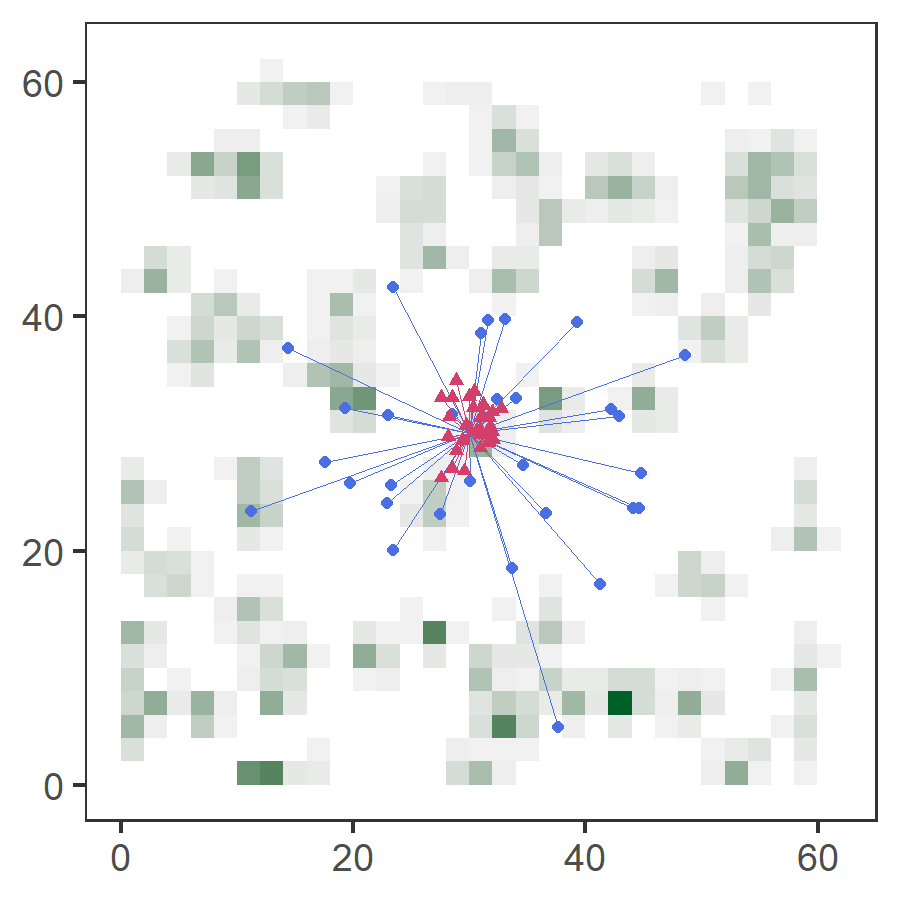
\includegraphics{figures/pathomove/fig_global_dispersal.png}
    \caption{
        \textbf{Differences between local and global dispersal.} 
        Initialising individuals in each new generation within a standard deviation of 10 units around their parent (\textbf{blue}; parent at [30, 30]) places can lead them to encounter potentially very different ecological, and social, circumstances from those of their parent. In contrast, individuals initialised close to their parents (within a standard deviation of 2 units; \textbf{red}) encounter very similar conditions as their parent. The latter also leads to substantial competition among kin. We used 10 units to represent (nearly) global dispersal, and 2 units to represent local dispersal; this is controlled by the simulation parameter \emph{dispersal}, which takes a numeric argument.
    }\label{fig:patho_dispersal}
\end{figure}

\subsection*{Evolutionary Outcomes of the Global Dispersal Implementation}

In the global dispersal scenario (see Fig.~\ref{fig:patho_dispersal}), there is a marked difference in which social movement strategy is evolved before pathogen introduction.
Since individuals are initialised relatively far away from their parent's position, they encounter potentially very different ecological conditions, both in terms of the number of other individuals, and the local availability of food items.

As a result, most individuals evolve a `handler tracking' social movement strategy before the introduction of the novel pathogen.
This strategy allows individuals to gain the benefits of social information on the location of a resource patch (of which handlers are an indirect cue), while avoiding potential competitors, as well as potentially moving away from areas without many food items.

After pathogen introduction, there is a rapid evolutionary shift in social movement strategies, similar to the shift seen in our default implementation of local dispersal.
However, these shifts only occur under conditions where the cost of infection is apparently greater than the value of using social information to find food items.
In brief, \emph{(1)} when the benefits of social information cannot compensate for the costs of infection risk ($\delta E$ = 0.5; $\delta E$ = 0.25, and R = 1, 2), the agent avoiding strategy becomes more prevalent, similar to the local dispersal case. \emph{(2)} When the costs of infection are lower than the benefits of social information, or when the resource landscape's productivity can offset the cost of infection, the handler tracking strategy persists as the dominant strategy (see Fig.~\ref{fig:patho_evo_global}).

\begin{figure}
    \centering
    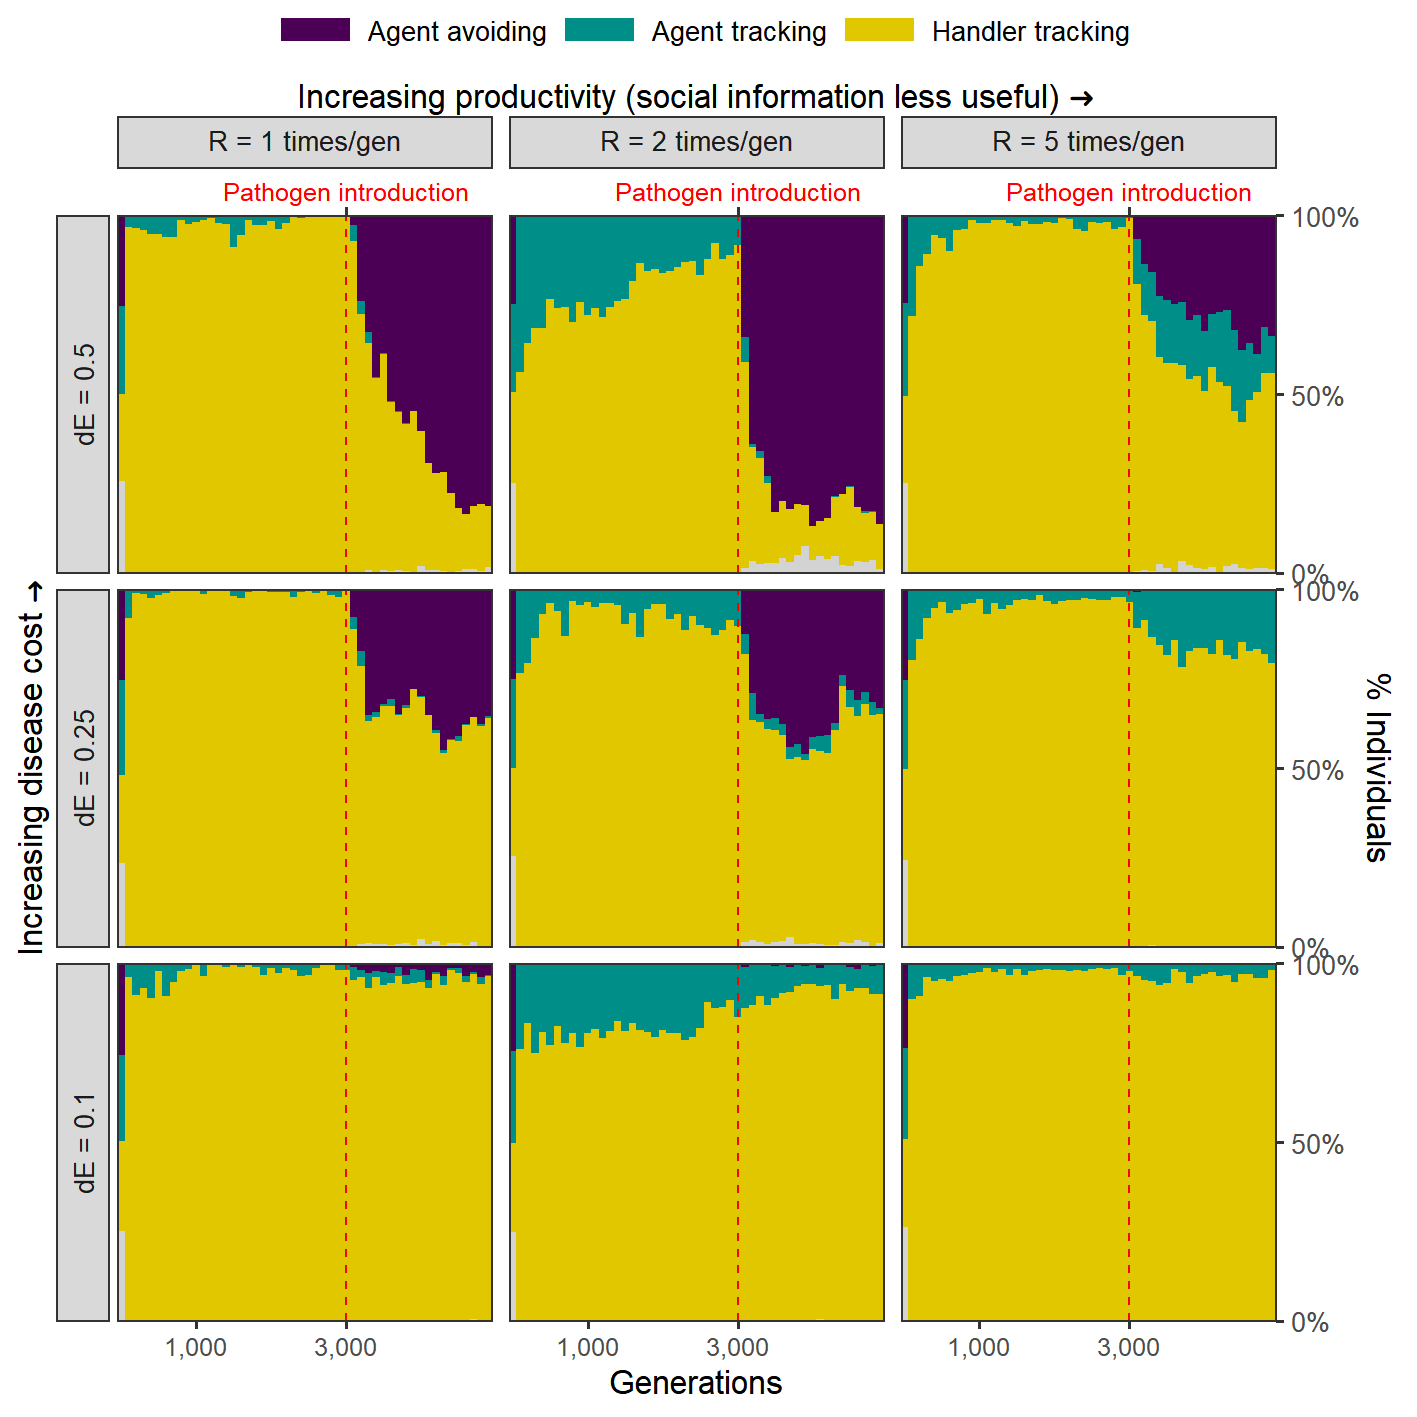
\includegraphics[width=0.9\textwidth]{figures/pathomove/fig_evo_change_global_dispersal.png}
    \caption{
        \textbf{Pathogen introduction triggers similar evolutionary changes under global dispersal as under local dispersal.} In our alternative, global natal dispersal implementation, the handler tracking strategy is the dominant strategy across most parameter combinations prior to pathogen introduction. Following pathogen introduction, there is a rapid shift in the mix of movement strategies under some ecological conditions. When the cost of infection is greater than the apparent benefit of social information, the agent avoiding strategy becomes more common. When infection costs are low ($\delta E$ = 0.1), pathogen introduction does not alter the mix of movement strategies, and the handler tracking strategy continues to be the most common strategy.}
    \label{fig:patho_evo_global}
\end{figure}

\subsection*{Ecological Consequences in the Global Dispersal Implementation}

In the global dispersal implementation, there is little to no change in population-level ecological outcomes --- mean distance moved, mean per-capita intake, and the mean number of associations --- following pathogen introduction (Fig.~\ref{fig:patho_global_eco}).
This is despite the drastic shift in evolved social movement strategies.
This is likely because a large part of individual's lifetimes (at low $R$, up to 90 timesteps), are spent moving, likely to find resource clusters.
Since intake depends on finding these clusters, and associations mostly take place at or near resource clusters, these are also reduced compared to our local dispersal implementation.

\begin{figure}
    \centering
    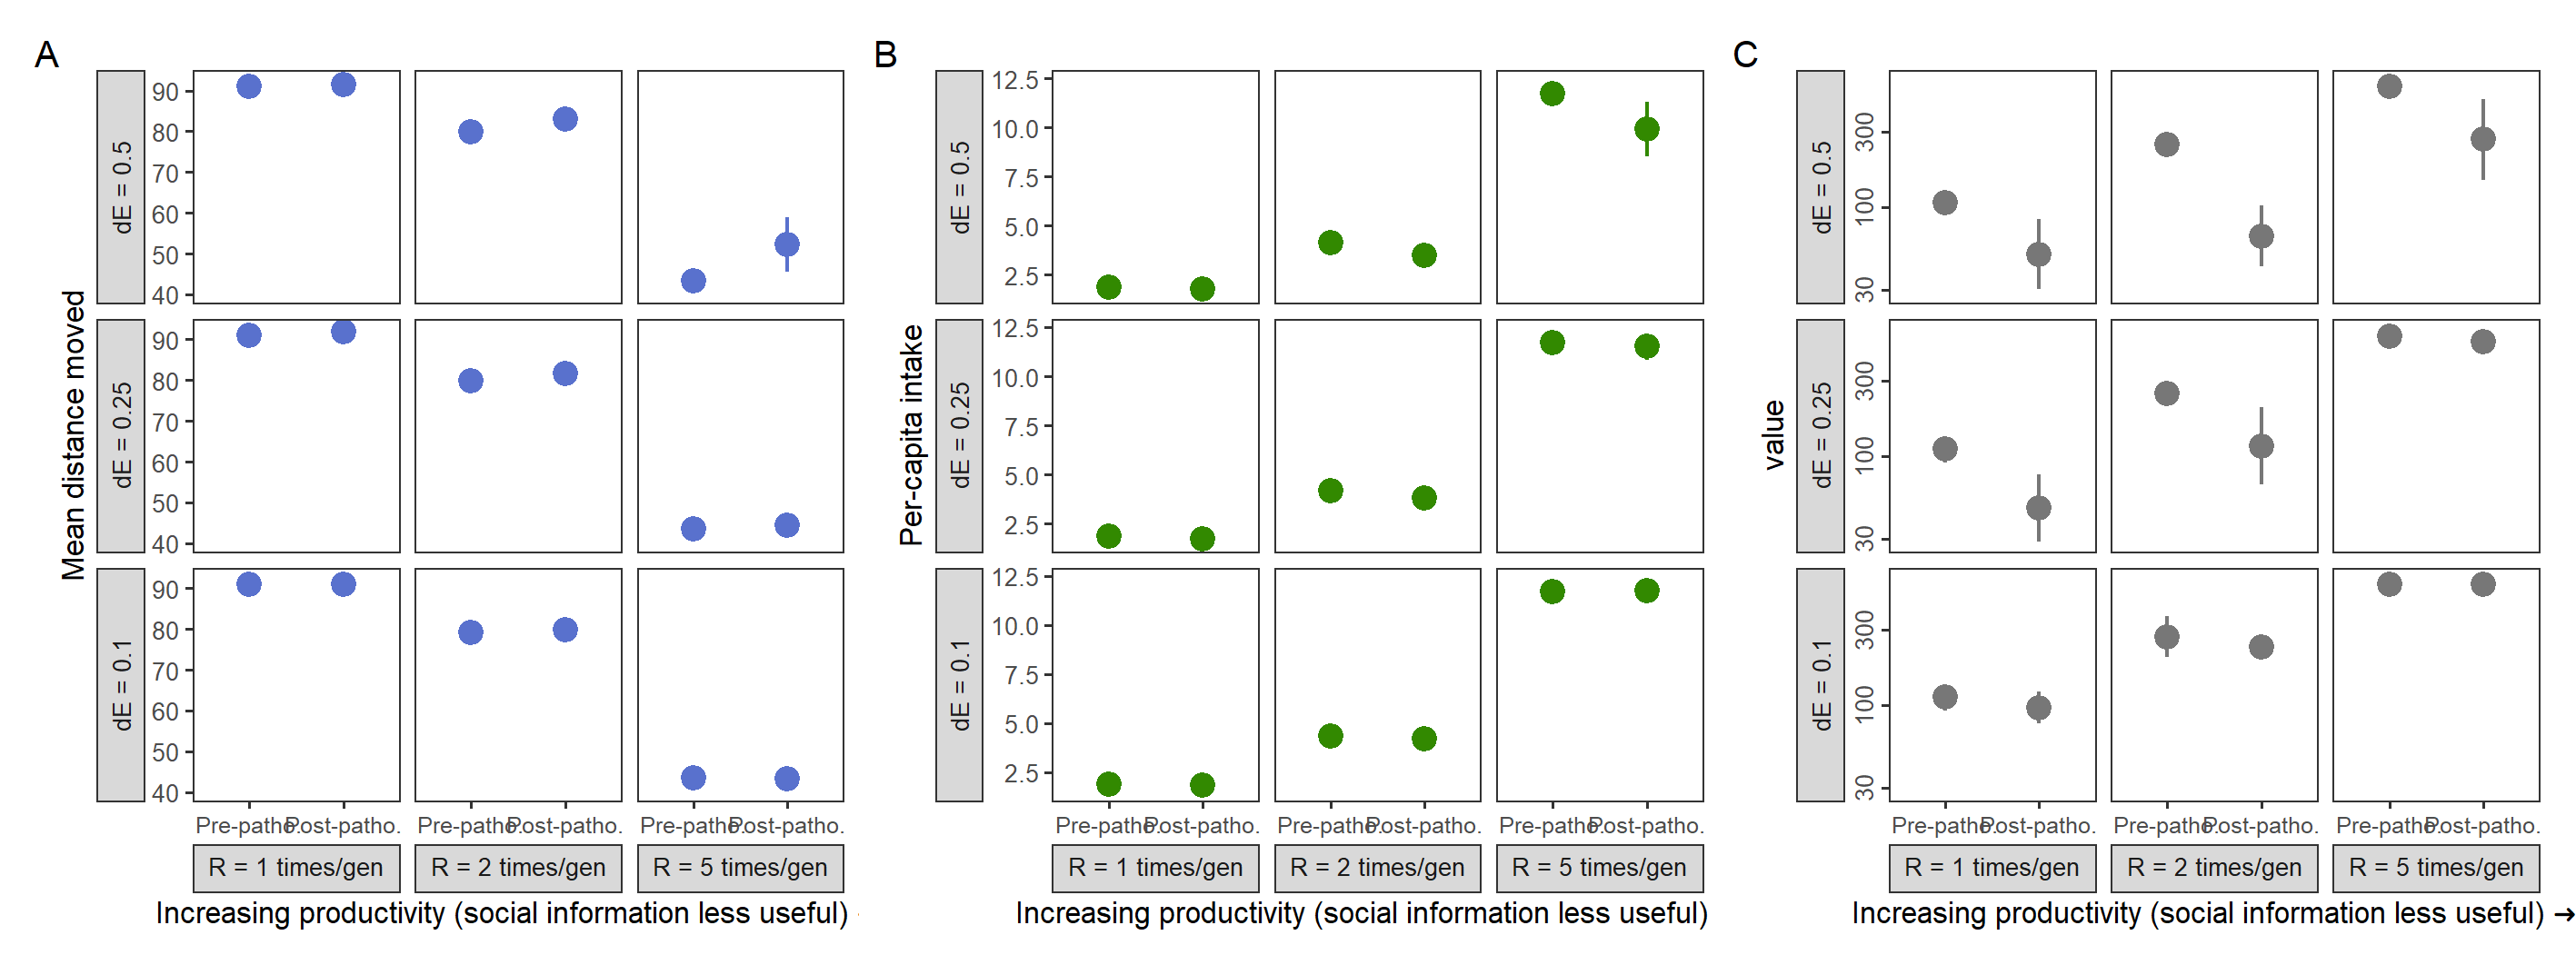
\includegraphics[width=0.95\textwidth]{figures/pathomove/fig_eco_compare_global.png}
    \caption{
        \textbf{Little to no change in ecological outcomes when implementing global dispersal.} Despite strong and rapid evolutionary shifts in social movement strategies, the ecological outcomes for populations with global natal dispersal are very similar before and after the introduction of the infectious pathogen. Each subplot in each panel shows the mean and standard error of the per-capita values for \textbf{(A)} distance moved, \textbf{(B)} intake, \textbf{(C)} number of associations, or encounters, with other individuals. Means and standard deviations are shown before (G = 3,000) and after (G = 3,500) pathogen introduction; each data point represents 10 replicates of the relevant parameter combination.
    }\label{fig:patho_global_eco}
\end{figure}

\subsection*{Infection Cost as a Percentage of Intake}

In our model's default implementation, the infectious pathogen imposes a direct cost, $\delta~E$, on individuals, in each timestep that they are infected.
For an individual with intake $N$, the net energetic gain $E$ after being infected by a pathogen for $t$ timesteps is $E = N - (\delta E \times t)$.
In this scenario, \emph{infection costs are independent of intake}.

In an alternative implementation, the infectious pathogen may be considered to reduce an animal's ability to process intake, or to require a portion of daily intake to resist.
Such an implementation is used in \ldots{}
For an individual with intake $N$, the net energetic gain $E$ after being infected by a pathogen for $t$ timesteps is $E = N \times (1 - \delta E) ^ t$.
Naturally, the two cost structures are not easy to compare, but a comparison of the potential outcomes is shown in Fig.~\ref{fig:compare_cost_structure}.

\begin{figure}
    \centering
    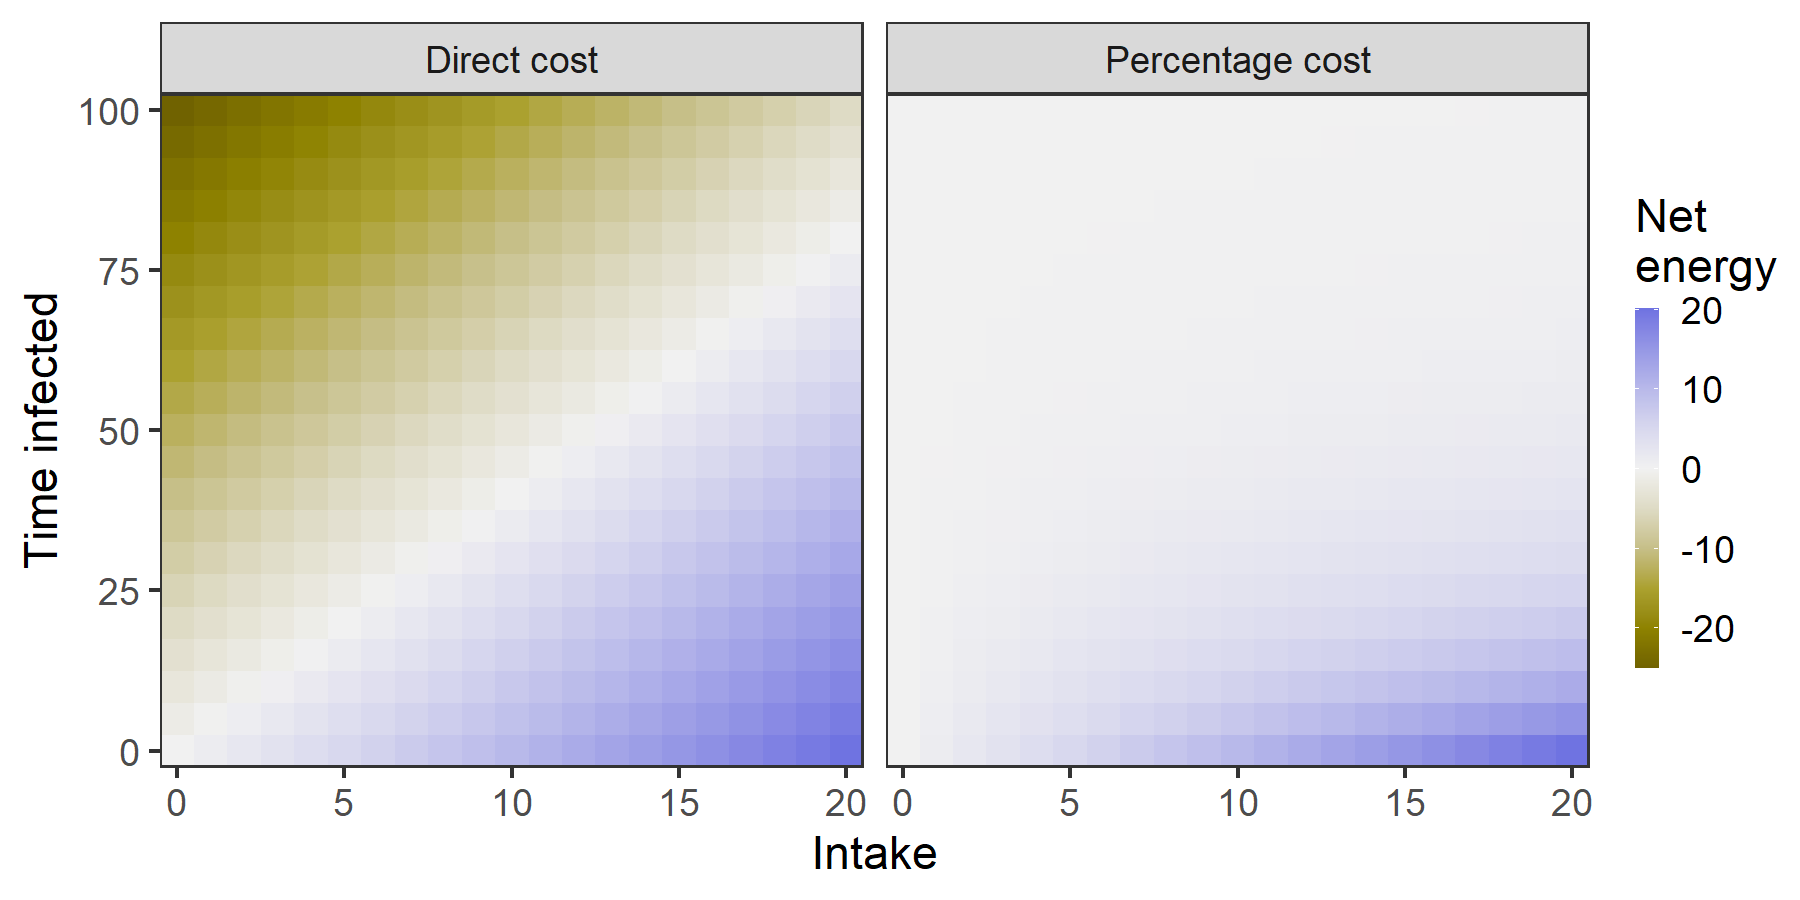
\includegraphics[width=0.7\textwidth]{figures/pathomove/fig_cost_structure.png}
    \caption{
        Calculated net energy for different combinations of intake and time infected. 
        In the \emph{Direct cost} scenario, and with a $\delta~E$ of 0.25 (shown here), which is our default implementation, an individual foraging on an item (handling time = 5 timesteps) would gain 1.0 unit of intake, and lose 1.25 units of energy in that same period if it were infected, for a net energy balance in that period of -0.25. 
        Individuals' energetic balance is normalised (0 -- 1) with reference to the lowest value in each generation. 
        Here, individuals' infection cost is \emph{independent} of their intake. 
        In the \emph{percentage cost} scenario, individuals' infection costs are linked to their intake. 
        For a per-timestep 5\% loss of intake (shown here), individuals infected for $>$25 timesteps already have a net energy balance close to, but never less than, zero. 
        In this implementation, individuals' energy balances are \emph{not normalised} with reference to the lowest net energy, as no individual's energy is ever less than zero.
    }\label{fig:compare_cost_structure}
\end{figure}

\subsection*{Evolutionary Outcomes of the Percentage Cost Implementation}

The social movement strategies evolved prior to pathogen introduction are identical to those seen in our default implementation.
This is because the percentage cost implementation differs from the default only after the pathogen is introduced.
After pathogen introduction, there is a rapid evolutionary shift in movement strategies.
This shift is similar to that in our default implementation, but the strategies evolved are different.
The handler tracking strategy becomes common across parameter combinations.
However, when the costs of infection are relatively high (7.5\%), and the usefulness of social information is limited by the abundance of food items (R = 5), the agent avoiding strategy forms about one fourth of the population mixture of social movement strategies

\begin{figure}
    \centering
    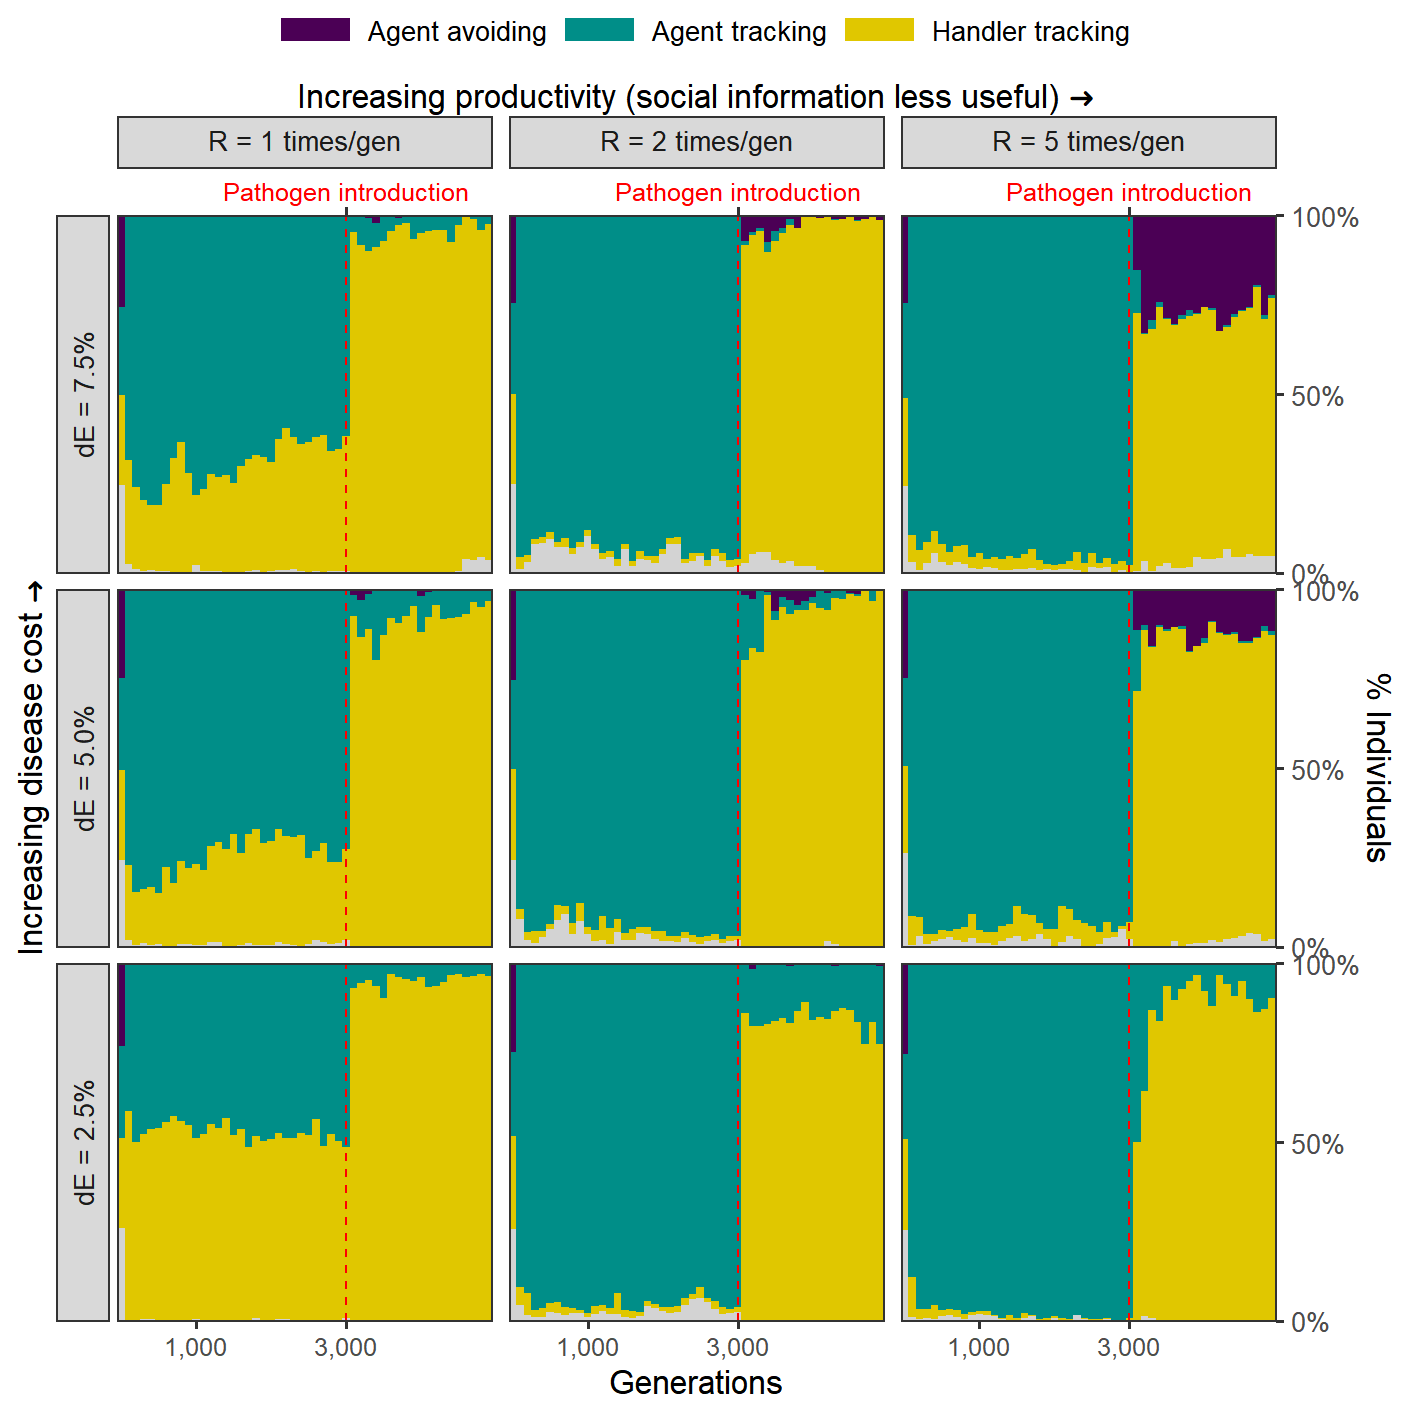
\includegraphics[width=0.9\textwidth]{figures/pathomove/fig_evo_change_percent_cost.png}
    \caption{
        \textbf{Rapid evolutionary change, but different evolutionary outcomes, in an alternative implementation of disease costs.} In our alternative, percentage costs implementation of the infectious pathogen, there is a rapid shift in the mix of movement strategies after pathogen introduction. The handler tracking strategy becomes common across all parameter combinations. Only when the costs of infection are relatively high (7.5\%), and the usefulness of social information is limited by the abundance of food items (R = 5), does the agent avoiding strategy form about one fourth of the population mixture of social movement strategies.
    }
\end{figure}

\subsection*{Ecological Consequences in the Percentage Cost Implementation}

Surprisingly, the implementation of a different cost structure for the novel, infectious pathogen does not affect ecological, population level outcomes when compared with outcomes in our default implementation of direct costs.
Across parameter combinations where there is a rapid evolutionary transition from agent tracking to handler tracking as the dominant strategy, there is also an increase in distance moved, a reduction in intake, and a reduction in associations.
Notably, the reductions in per-capita intake following pathogen introduction are similar to a halving of landscape productivity (as in the default implementation), and there is a comparable drop in the number of pairwise associations among individuals.

\begin{figure}
    \centering
    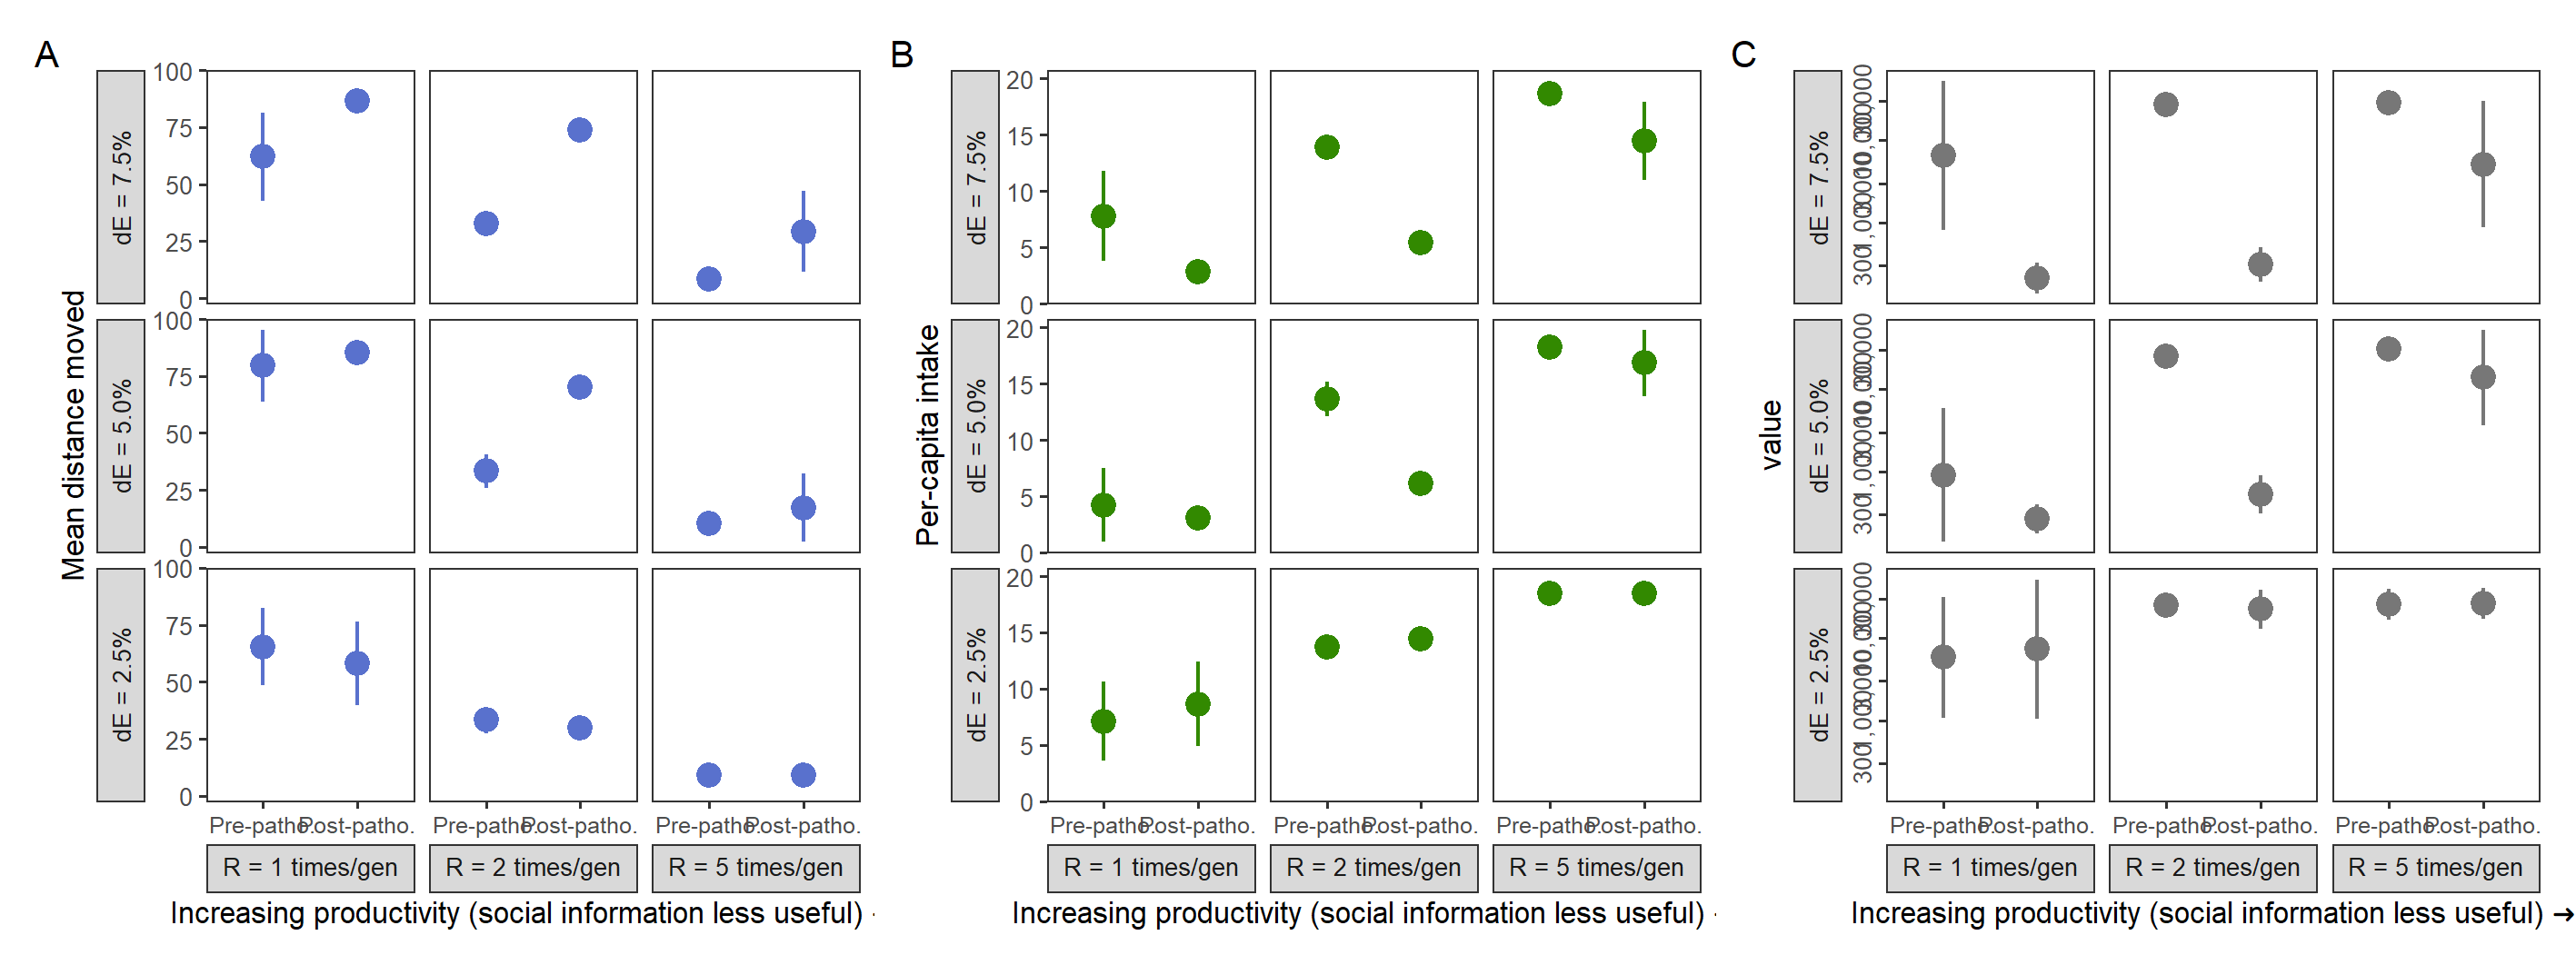
\includegraphics[width=0.95\textwidth]{figures/pathomove/fig_eco_compare_percent.png}
    \caption{
        \textbf{Rapid ecological changes accompany evolutionary shifts in an alternative implementation of disease costs, and are similar to the default implementation.} In the alternative percentage-costs implementation of the infectious pathogen, the outcomes are very similar to those in our default implementation of direct costs. Across most parameter combinations, there is an increase in movement, a reduction in intake, and a reduction in associations with other foragers. Each subplot in each panel shows the mean and standard error of the per-capita values for \textbf{(A)} distance moved, \textbf{(B)} intake, \textbf{(C)} number of associations, or encounters, with other individuals. Means and standard deviations are shown before (G = 3,000) and after (G = 3,500) pathogen introduction; each data point represents 10 replicates of the relevant parameter combination.
    }
\end{figure}

\subsection*{Sporadic Introduction of Infectious Pathogens}

We implemented a variant of our main model, in which the infectious pathogen is introduced only sporadically after the first introduction event (at G = 3,000).
Specifically, we modelled probabilistic introduction of the pathogen in each generation following the initial introduction.
We call the per-generation probability of a novel pathogen introduction event the `spillover rate'.
We ran 10 replicates each of this model variant and examined whether there was a similar evolutionary shift in social movement strategies as seen in our default implementation.
Since it is the main parameter of interest, we ran this model variant for three values of the spillover rate: 0.05, 0.1, and 0.25.
Instead of examining the joint effect of landscape productivity and cost of infection as well, we only examined the effect of infection cost, implementing three different variants with an infection cost \(\delta E\) of 0.1, 0.25, and 0.5.
We kept all other model parameters similar to the default scenario of our main model, and importantly, considered only a landscape productivity \(R\) of 2.
Cross-species novel pathogen introductions are likely to become more common with climate change, and so we chose these spillover rate values to represent different scenarios under altered global regimes of pathogen transfer.
Our model's default implementation may be seen as an extreme case of the models considered here, with a spillover rate of 1.0.

In our model code, the sporadic introduction is implemented by drawing the number of generations until the next pathogen introduction event from a geometric distribution whose probability parameter is given by the spillover rates described above.
Zero values are handled by converting them into ones.
At our lowest spillover rate, up to 100 generations could pass between pathogen introductions, while at our highest rates, there are rarely more than 10 generations between introductions.

The social movement strategies evolved prior to pathogen introduction are identical to those seen in our default implementation, as expected.
However, following pathogen introduction, we found that there was little to change in the population-level mixture of movement strategies in this model variant (see figure).
This is regardless of the probability of a novel pathogen introduction (our so-called `spillover rate'), and the cost of infection by a pathogen.
Across the simulation, the commonest social movement strategy remains `agent tracking', i.e., preferring locations with multiple individuals regardless of their foraging status.
Since there is little to no change in social movement strategies, we did not expect nor find changes in ecological outcomes.

\begin{figure}
    \centering
    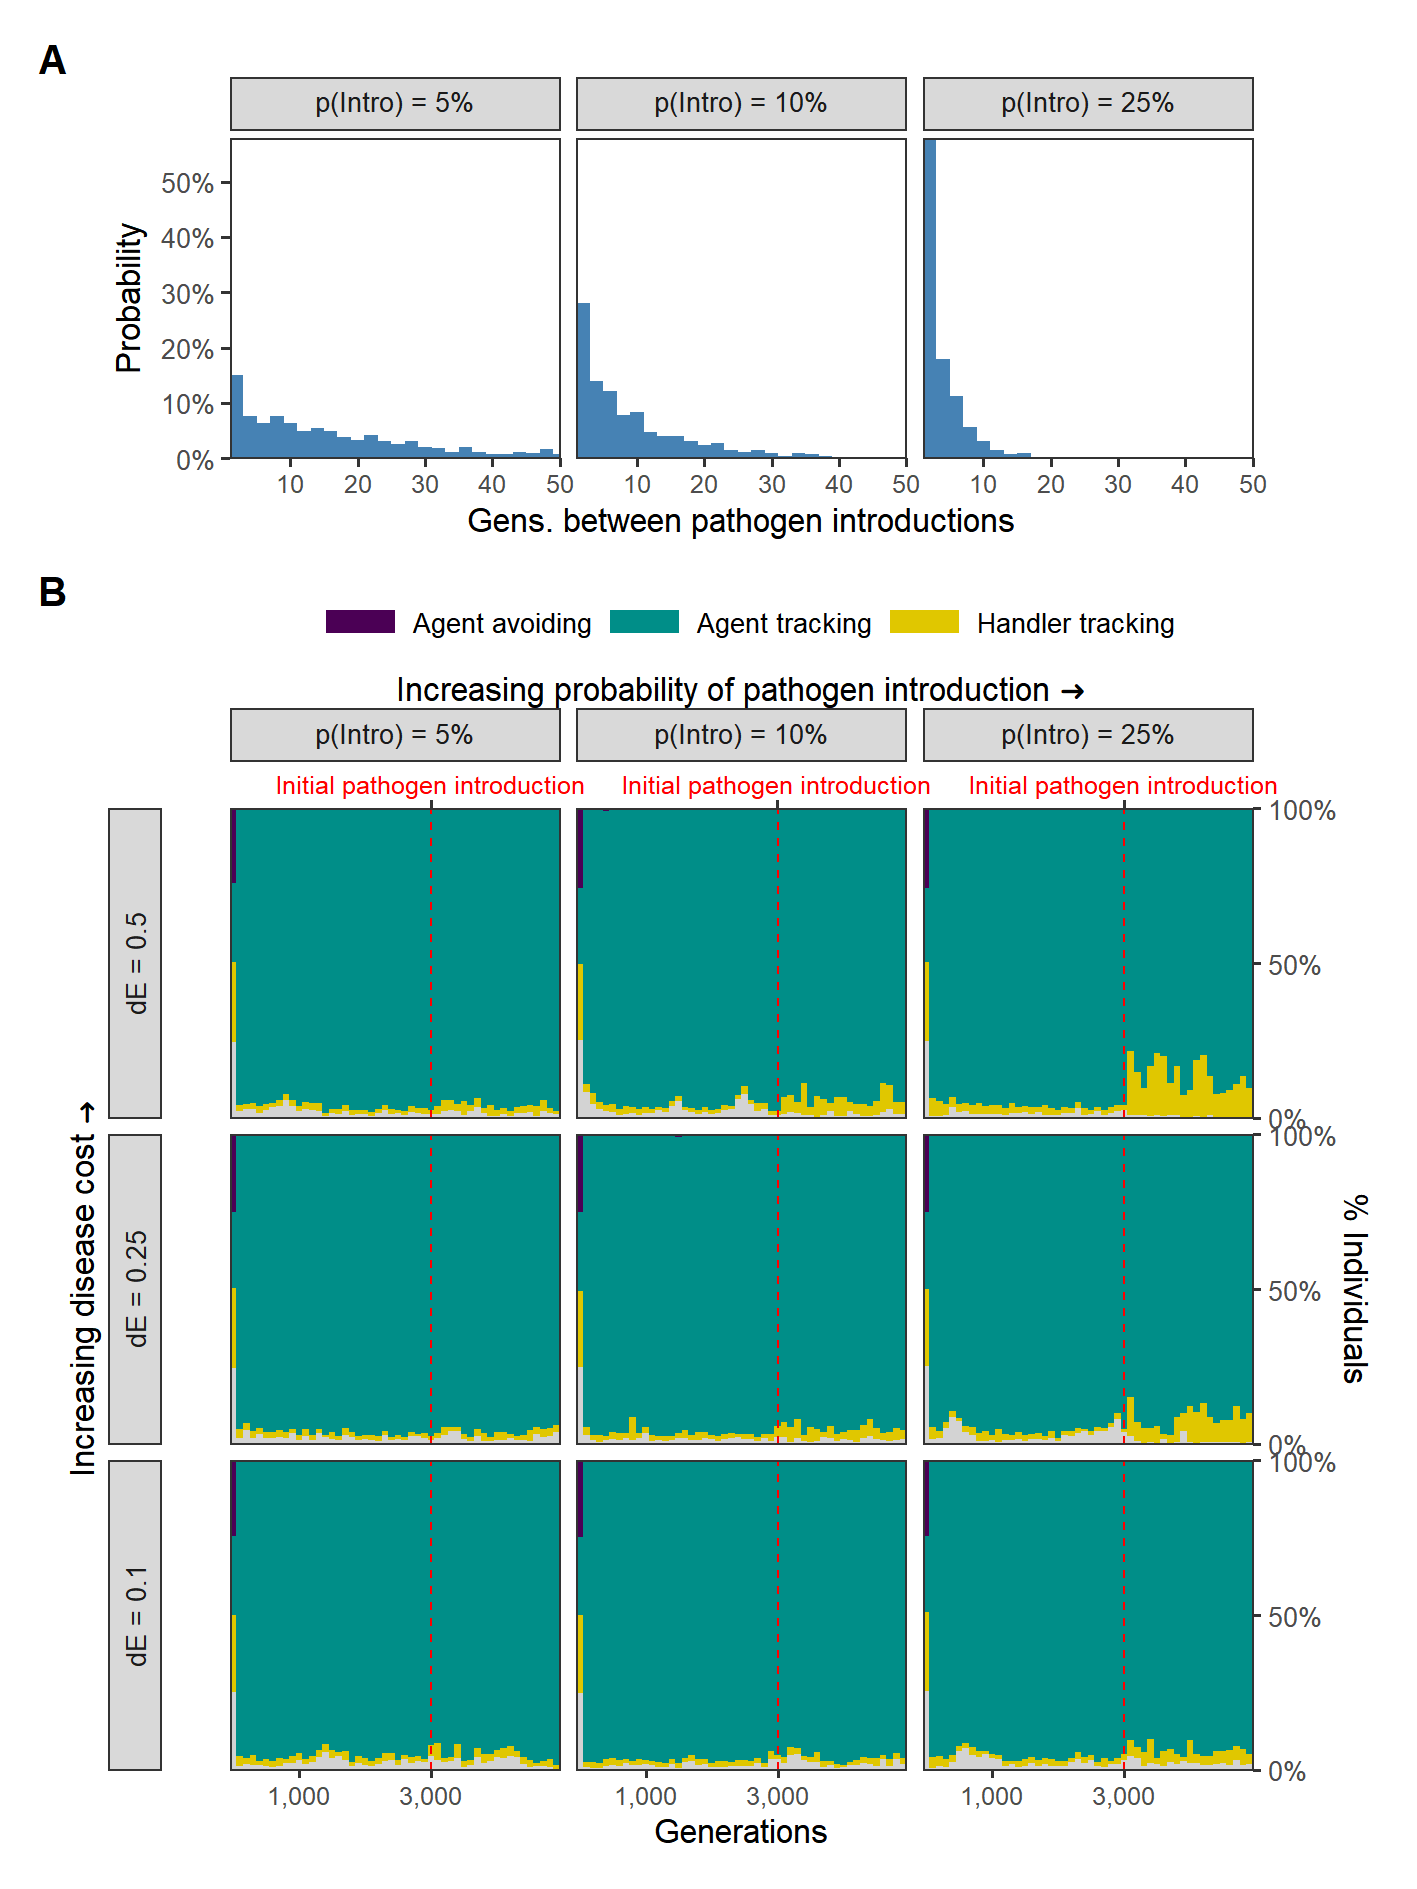
\includegraphics[width=0.7\textwidth]{figures/pathomove/fig_evo_strategy_sporadic.png}
    \caption{\textbf{No evolutionary change in social movement strategies when novel pathogen introduction events are relatively uncommon.} \textbf{(A)} In our alternative implementation of the model, the pathogen is only introduced sporadically after the initial introduction (G = 3,000; red line in panel B). \textbf{(B)} When the introductions are relatively rare and sporadic, there is no shift in the mixture of movement strategies after pathogen introduction. The agent tracking strategy remains common across parameter combinations.}
\end{figure}

{ \begin{center} \barfont{-.-} \end{center} }

\endgroup



\cleardoublepage 
%************************************************
\addtocontents{toc}{\protect\vspace{\beforebibskip}}%
\chapter{Using a Mechanistic Model to Probe Statistical Methods in Animal Movement}\label{ch:patternprocess}
\chaptermark{Probing Statistical Models}
%************************************************

{\noindent \textbf{Pratik R. Gupte} and Franz J. Weissing}

\section*{Abstract}

% \small{
    Movement ecologists have taken up the challenge of inferring animals' decision-making mechanisms in a spatial context from individual tracking data.
    The implicit assumption is that differences in the movement paths of animals reflect differences in individual decision-making mechanisms.
    However, animal movement takes place in complex and rapidly changing environments, where movement cues are not always available, and animals may differ along multiple axes of behaviour.
    Mechanistic, individual-based modelling of animal decision-making can help investigate whether differences in decision-making mechanisms actually translate into differences in movement paths, and the insights gained by parsing animal tracking data using contemporary statistical methods.
    Here, we examine the movement paths of agents from an evolutionary individual-based model of foraging competition, in which relatively simple movement rules are determined by evolved decision-making weights.
    To show how such a model can be used to investigate statistical methods, we explore a contemporary question in movement ecology: Can individual differences in movement decision-making mechanisms be detected from the emergent properties of the resulting movement paths?
    % First, we examine whether our model individuals' movement types differ in the structure of their movement paths.
    Using data on the movement of evolved model agents, we show how adopting a repeatability framework to quantify individual-differences in movement is sensitive to the evolutionary context in which movement rules evolve.
    We also find that repeatability analysis can yield very different conclusions depending on how individuals' behavioural types are accounted for.
    We also show that step-selection analysis can indicate differences between competition strategies, but rarely captures differences between movement types of the same competition strategy.
    Overall, using a plausible eco-evolutionary model of animal decision-making, we highlight some challenges in using contemporary statistical methods to infer individual differences in animals' decision-making mechanisms from positioning data.

    \bigskip

    {\noindent \large{$\Delta$}} A manuscript in preparation.
% }

\clearpage


% \newrefcontext[sorting=ynt]

    \lettrine{A}{nimal} movement is understood to be an individual response that integrates multiple internal and external stimuli, including environmental conditions and the presence of other animals \citep{nathan2008a}.
    Various aspects of animal movement, such as the distance moved over time (speed), or the tortuosity of an animal's path, are now readily measured and quantified in free-living individuals, given significant advances in animal tracking technology \citep[][see Nathan et al. \textit{in prep.}]{cagnacci2010}.
    This makes movement a sort of `model behaviour' that allows investigation of the underlying mechanisms --- the `how' and `why' of animal decision-making --- under natural conditions that cannot be replicated in experimental settings.
    For example, tracking individual greenbuls \textit{Phyllastrephus sp.} in forested landscapes revealed that greenbuls moved more frequently to trees that were actually visible from their position, rather than trees that were obscured from view, indicating that visual cues are important in the movement decisions of forest birds \citep[][see also \citep{aben2018}]{aben2021}.
    This illustrates a general tactic in animal movement studies, which is to treat an animal's use of a resource disproportionate to its availability \citep{manly2007,fortin2005,signer2019}, or prolonged residence in an area \citep{bracis2018} as indicators of adaptive movement decision-making mechanisms.
    Simple simulation models show that differences in movement patterns --- such as path metrics, or emergent social interactions --- may reflect underlying differences in movement strategies \citep{spiegel2017}.
    
    Both differences in movement strategies, or the mechanisms controlling movement \citep{spiegel2017}, and differences in movement paths, which are the outcomes of movement mechansims \citep{abrahms2017,hertel2021}, are interpreted as facets of animal personality \citep{sih2004,sih2004a}.
    Increasingly however, animal personality, or consistent individual differences in behaviour, are studied in empirical terms, and considered to be detected in a population when its behavioural responses possess certain statistical properties \citep{sanchez-tojar2021}.
    In the context of animal movement, researchers apply sophisticated variance-partitioning approaches to common movement metrics --- such as daily distance moved --- and aim to determine how much behavioural variation in a population is explained by individual identity, rather than conditions that directly influence behaviour (e.g. diel cycle, temperature), or variation due to other, un-examined factors (e.g. weather differences between intervals) \citep{hertel2020, hertel2019, hertel2021}.
    Another approach to investigate individual animals' decision-making mechanisms is to estimate their relative preferences for environmental conditions using step-selection analysis \citep[][see also resource selection analysis: \citealt{manly2007}]{fortin2005,thurfjell2014,avgar2016,signer2019,fieberg2021}.
    Step-selection analysis compares environmental cues between animals' real steps --- the movements actually made, and their alternatives --- the movements that \textit{could have been made}, from the same starting location \citep{thurfjell2014,fieberg2021}.
    The relative selection strengths, which are the coefficients of a step-selection function, can be compared between individuals \citep{thurfjell2014}, and should be expected to be different for individuals with different movement decision-making mechanisms.
    
    However, it is unclear whether individual consistency in the mechanisms underlying movement strategies can really be identified using current statistical tools.
    Most researchers realise that there is a substantial gap between the environment animals perceive and to which they respond, and the often static representation of that environment that is measured in tracking studies.
    For example, resources that are critical to animals are often ephemeral, and difficult to measure with both a high spatio-temporal extent and resolution using existing technologies such as remote sensing, leading researchers to fall back on more long-term resource proxies such as vegetation indices \citep{pettorelli2011}.
    This issue is likely even more acute in the case of movements that have a social context, such as competition, as the social environment is expected to change even more rapidly than resource distributions, and to be even more sensitive to local consumer densities.
    Consequently, it may be difficult to determine whether differences in movement reflect underlying differences in decision-making mechanisms, or whether they better represent stochastic differences in environmental conditions encountered by animals.
    Applying current methods in animal movement ecology to individual-based simulation models of animal movement strategies \citep[see e.g.][]{getz2015,getz2016,netz2021} can help explore whether these methods can reliably detect individual differences in movement decision-making mechanisms.
    
    Mechanistic models of intermediate complexity can simulate the main features of many spatial systems, such as heterogeneity in landscape productivity, and resource depletion due to mobile consumers \citep{getz2015,white2018,deangelis2019,netz2021,diaz2021}.
    Here, we work with an evolutionary, individual-based model of agent movement in the context of intraspecific competition (both exploitation and interference, as described in Chapter~\ref{ch:kleptomove}).
    In our model, agent movement is the outcome of the interplay of simple movement decision-making mechanisms, a fluctuating resource landscape, and due to agent movement, a variable social landscape.
    % Agents can be programmed to move according to specific movement rules, which are controlled by 
    Agent movement strategies are controlled by their preferences for environmental cues, such as resource and competitor densities \citep[see e.g.][]{getz2015,white2018,netz2021}.
    % The movement weights are used to assess the fluctuating resource landscape, as well as changing local densities of competitors.
    These preferences may be thought of as the coefficients of resource- or step-selection functions \citep[][]{white2018}.
    Importantly, in contrast with purely ecological models \citep[e.g.][]{white2018}, agents' preferences are outcomes of many generations of natural selection \citep[see also][]{getz2015,netz2021}.
    We previously showed that in two scenarios of exploitation and interference competition, differences among individuals in how they assess local environmental cues evolve.
    % Consequently, we would expect to see these differences in mechanisms reflected in the structure of emergent movement paths.
    
    We tackle three specific aspects of a general question in animal movement: what can applying statistical tools to animal tracking data tell us about individual differences in the movement decision-making mechanisms?
    \textit{(1)} We first examine whether different movement types are indicated by simple exploratory data analysis.
    \textit{(2)} We then investigate the results of a variance-partitioning approach (repeatability analysis; \citealt{nakagawa2010,hertel2019}) to detecting individual differences in populations with different movement types \textit{and} competition strategies.
    % \textit{(2)} Are decision-making mechanisms good predictors of the structure of the paths they generate? Can environmental predictors better explain movement path structure?
    \textit{(3)} Finally, we attempt a novel application of step-selection analysis to the study of consistent individual differences in movement strategies.
    Overall, by treating a simulation model with simple movement rules as we would empirical animal-tracking data, we aim to explore whether individual differences in movement decision-making mechanisms can be reliably inferred from the emergent structure of animal movement paths.
    
    \section*{Methods}
    
    \subsection*{Basic Model Setup}
    
    We worked with an individual-based evolutionary simulation model of animal movement in a foraging context, previously developed for use in Chapter~\ref{ch:kleptomove}.
    We describe the model's ecological dynamics in brief here, and refer readers to Chapter~\ref{ch:kleptomove} for a more detailed exploration of the evolutionary outcomes.    
    Our model simulates a population with a fixed size (10,000 individuals), moving on a finely gridded landscape of 512\textsuperscript{2} cells; this is a population density of 1 individual for every 26 cells.
    The landscape is wrapped at the boundaries so that individuals passing beyond the bounds at one end re-appear on the diametrically opposite side.
    The model consists of $G$ generations (default = 250) of $T$ timesteps (default = 400); in each generation, individuals move and make foraging decisions to gain intake.
    % , and is also an important mechanism influencing the structure of individual movement paths.
    At the end of each generation, individuals reproduce and pass on their movement and foraging strategies to their offspring, the number of which is proportional to their intake in the 400 timesteps of their `lifetime'.
    
    The cells of the gridded landscape each have a cell-specific probability $r$ of generating a discrete resource, which we refer to as `prey items' (e.g. a mussel).
    The cells are arranged into 1,024 regularly spaced clusters, or `resource peaks', in which the productivity of cells at the centre of the peak (called $r_{max}$) is five times greater than the cells at the periphery of the peak; resource peaks are approximately 16 cells away from each other.
    We ran the model with a default $r_{max}$ of 0.01, and also at $r_{max}$ values between 0.001 and 0.03, to examine the effect of landscape.
    For an $r_{max}$ = 0.01, the most productive cells (at the centres of a cluster) are likely to generate one item per 100 timesteps (or four items per generation, for $T$ = 400), while the least productive cells (at cluster peripheries) are likely to generate one item every 500 timesteps ($<$ than one item per generation, for $T$ = 400).
    Cells in our landscape were modelled as having a uniform carrying capacity $K$ of 5 prey items, and while a cell is at carrying capacity its $r$ is 0.
    
    \subsection*{Individual Foraging and Movement}
    
    Agents can perceive a cue indicating the number of all prey items $P$ in a cell, but have a probability $q$ of failing to detect a prey item, and a probability $q^P$ of not detecting any of $P$ prey items; foragers are thus successful in finding a prey item with a probability $1 - q^P$.
    Individuals on a cell forage in a randomised sequence, and the probability of finding a prey item ($1 - q^P$) is updated as individuals find prey, reducing $P$.
    Foragers that are assigned a prey item in timestep $t$ begin handling it, and are considered to be handlers for the next $T_H$ timesteps, during which they are immobile: this creates opportunities for kleptoparasitism \citep{holmgren1995}.
    Foragers that are not assigned a prey item are considered idle, and are counted as non-handlers.
    
    Agent movement is a fine-scale process comprised of small, discrete steps of fixed size.
    These steps are the outcome of short-term individual movement decisions, in which the agent selects a destination cell, after assessing potential destinations based on available cues \citep[similar to step selection or resource selection][]{fortin2005,manly2007}, an approach used previously by \cite{getz2015} and \cite{white2018}.
    In brief, individuals scan the nine cells of their Moore neighbourhood for three environmental cues, \textit{(1)} an indication of the number of discrete prey items $P$, \textit{(2)} the number of individuals handling prey $H$ (called `handlers'), and \textit{(3)} the number of individuals not handling prey $N$ (called `non-handlers').
    Based on these cues, agents rank their neighbouring cells by their `suitability score' $S$, where $S = s_PP + s_HH + s_NN$, and move to the cell to which they have individually assigned the highest suitability.
    The weighing factors for each cue, $s_P$, $s_H$, and $s_N$, are genetically encoded and and transmitted from parents to their offspring.
    All individuals move simultaneously, and then implement their foraging strategy to acquire prey.
    
    \subsection*{Scenarios of Intraspecific Competition}
    
    We considered two scenarios of intraspecific foraging competition, a process that can strongly shape animal movement and population distributions \citep{fretwell1970,parker1978}.
    %%
    In the exploitation competition \textbf{scenario 1}, agents move about on the landscape according to their movement rules, and find, handle, and consume prey.
    Agents must handle each prey item for a fixed handling time $T_H$ (default = 5) before they gain its energetic value.
    Agents can be either in the handling or searching state \citep{holmgren1995}.
    While handling, agents are immobile and do not make any movements.
    Since there are no direct interactions among agents, the only way in which agents can affect each others' intake is by acquiring prey items before their competitors.
    In this scenario, the only evolvable properties are the environmental cue weighing factors which determine the suitability scores and hence agent movement ($s_P$, $s_H$ and $s_N$).
    
    In \textbf{scenario 2}, agents can either search for prey items (foraging), or steal a prey item from a handler (kleptoparasitism).
    Agents make movement decisions as in the exploitation competition scenario, but their competition strategy (foraging or kleptoparasitism) is fixed through life, genetically encoded, and heritable between generations.
    For simplicity, agents are always successful in stealing from a handler; however, if multiple agents target the same handler, only one of them, randomly selected, is considered successful --- thus kleptoparasitic agents also compete exploitatively among themselves.
    %%
    Handlers that have been stolen from subsequently `flee' and are moved to a random cell within a Chebyshev distance of 5.
    Having acquired prey, a kleptoparasite converts into a handler, but need only handle prey for $T_H - t_h$ timesteps, where $t_h$ is the time that the prey has already been handled by the previous handler; thus kleptoparasites save time on handling compared to a forager.
    Unsuccessful kleptoparasites are considered idle, and are also counted as non-handlers.
    Handlers that finish processing their prey in timestep $t$ return to the non-handler state and are assessed as such by other individuals when determining their movements.
    
    \subsection*{Inheritance of Movement and Competition Rules}
    
    For simplicity, we modelled discrete, non-overlapping generations, with haploid, asexually reproducing individuals.
    In the exploitation competition scenario, individuals have three active gene loci that encode the decision-making weights which control individual movement ($s_P$, $s_H$, $s_N$). 
    In scenario 2, individuals additionally inherit their competition strategy from their parent.
    % four further weights for foraging decisions ($w_P$, $w_H$, $w_N$, $w_0$) are also active.
    We assume that the expected number of offspring per individual is proportional to the individual's total lifetime intake of resources (hence resource intake is used as a proxy for fitness). 
    This is implemented as a weighted lottery (with weights proportional to lifetime resource intake) that selects a parent for each offspring in the subsequent generation \citep[see prior implementation in][]{netz2021}.
    %%
    Across scenarios, the movement decision-making weights are subject to independent random mutations with a probability of 0.001.
    The mutational step size (either positive or negative) is drawn from a Cauchy distribution with a scale of 0.01 centred on zero.
    This allows for a small number of very large mutations while the majority of mutations are small.
    In scenario 2, agents have a probability of 0.001 of a mutation on their competition strategy, i.e., of transforming from a forager to a kleptoparasite, or vice versa.
    Agents are intialised at a random location on the landscape, potentially forcing individuals to contend with different environmental conditions from those experienced by their parent.
    
    \subsection*{Agent Positions, Agent Preferences, and Landscape Data}
    
    We previously established that in our model, the mean per-capita intake stabilises within 50 generations, and the fixation of certain movement rules (such as the preference for handlers) is complete by generation 100 (see Fig. 1).
    % We expected that by generation 250, model populations could be considered to have been adapted to their environmental conditions and competition scenario for at least 200 generations (50 -- 250).
    We wanted to determine whether agent path structure, and specifically, the distance moved, also has a clear trajectory over generations.
    In order to do this, we focused on the positions of 1\% of the agents (N = 100) in each timestep, for every 10\textsuperscript{th} generation, up to generation 249 (25 generations, including \textit{G} = 249).
    Overall, we collected 400 $\times$ 100 $\times$ 25 = 1,000,000 positions over each simulation run.
    To apply methods commonly used in movement analyses, we let the final generation (\textit{G} = 250) run for 10,000 timesteps, and exported the positions of 100 agents in each timestep, for a further 10,000 $\times$ 100 = 1,000,000 positions.
    We also exported the decision-making weights for movement ($s_P$, $s_H$, $s_N$) for each agent in the exploitation competition scenario, as well as the foraging strategy-decision weights ($w_P$, $w_H$, $w_N$, $w_0$) for agents in the interference competition scenario; we aimed to later relate these weights to the structure of movement paths.
    
    Animal movement is strongly influenced by the landscape, and must be taken into account to accurately compare among individuals.
    The cell $r$ values may be seen as analogous to empirically measured long-term indicators of productivity, such as the normalised-difference vegetation index \citep[NDVI;][]{pettorelli2011}.
    We took the known, fixed $r$ values for each cell, and linked them to agent positions as environmental covariates.
    Animals likely cannot always sense underlying differences in the drivers of productivity of a resource landscape, but only an indicator of that productivity, such as prey items.
    Nonetheless, long-term measures are frequently used as predictors in step-selection functions, because they are often easy to measure, and do have a mechanistic link with animal movement.
    
    % Long-term measures of productivity are insufficient to recover agent preferences for fine-scale environmental cues, such as resource densities and the presence of competitors, using step selection functions.
    % This is both because (1) agents cannot sense $r$ directly, and (2) fluctuations in resource and competitor densities are related through complex feedbacks that are unlikely to be well correlated with $r$.
    % Thus, we took a very fine-scale approach to recording environmental data for the final generation (G = 250).
    % We exported `ecological snapshot' of the landscape in 250 timesteps (from T = 5,000 to T = 5,250); these snapshot contained counts of prey items, handlers, and non-handlers for each landscape cell.
    % In the interference competition scenario, the non-handler counts were split into separate counts for agents that were searching for food (foragers), and agents that were seeking to target a handler (kleptoparasites).
    % From this sequence of snapshots, we were able to determine the environmental cues available to agents while making movement decisions.
    
    \subsection*{Quantifying Model Ecological Outcomes}
    
    We first plotted the frequencies of the decision-making weights, scaled between -1 and +1 using a hyperbolic tangent tranform, over the 250 generations of each model run (see Fig. \ref{fig1}A).
    We then visually examined the population at the evolutionary equilibrium for functional differences in movement rules.
    Since distinct values, or morphs, of each weight might be correlated with distinct values of the other two weights, agents with seemingly different absolute values of the three weights could have the same relative preference for, or aversion to, a movement cue.
    We did this by normalising each of the agents' three movement weights relative to the sum of the absolute values of the weights:
    $W_i = W_i / (|s_P| + |s_H| + |s_N|)$, where $W_i$ is any one of the movement weights, $s_P$, $s_H$ or $s_N$.
    We refer to these normalised weight values (ranging from -1, avoidance, to +1 preference) as the relative preferences.
    Thus, for example, an agent prioritising movement towards handlers would have a normalised value for $s_H$ close to +1, and $s_P$ and $s_H$ $\equiv$ 0.
    To visualise the spread of agents over the trait space, we plotted the scaled values of $s_H$ against the scaled values of $s_P$, colouring points by the scaled value of $s_N$ (see Fig. \ref{fig1}A).
        
    We classified the 100 agent paths exported in each simulation run based on the agents' relative preferences: (1) \textit{prey tracking}, if $s_P > 0.55$; (2) \textit{handler tracking}, if $s_H > 0.5$; (3) \textit{prey \& handler tracking}, if $s_P > 0,~s_H > 0,~|s_P - s_H| > 0$; (4) \textit{non-handler avoiding}, if $s_N < -0.5$; (5) \textit{handler avoiding}, if $s_H < -0.5$; and (6) \textit{mixed}, for all other combinations.
    We plotted the distribution of total distance moved across equal intervals for each of these five strategies (or those present in the evolved populations; see Fig. \ref{fig3}).
    We also plotted the movement paths of individuals from the strategies for a visual comparison of path structure and distance moved.
    
    \subsection*{Repeatability of Agent Movement}
    
    When animals are challenging to assay in captivity, researchers may attempt to detect individual consistency in movement behaviour from animal tracking data alone \citep[see a review in][see \citealt{hertel2019} for an example]{hertel2020}.
    In this approach, a population is understood to comprise of `repeatable' individuals if the between-individual variance in behaviour is a substantial proportion of the total variation that is not explained by the fixed effects of a linear mixed model \citep[LMM][]{hertel2019}.
    Individuals differing in behavioural mechanisms are expected to make differing movement decisions when presented with the same environmental cues; the cumulative and emergent effects of these decisions are thus expected to be reflected in the tracking data.
    Consequently, a population with differences among individuals in movement decision-making mechanisms (`movement types') should be expected to be `repeatable' in movement behaviour.
    This approach relies on repeated measures of an individual behaviour, such as daily distance moved \citep[][]{niemela2018, hertel2020}.
    One way of obtaining such repeated measures is by summarising behaviour over equal time-intervals of an animal's track \citep[see e.g.][]{hertel2019}.
    We investigated whether our agents' fixed movement decision-making weights would result in high population-wide repeatability in movement behaviour, and specifically, in the mean distance moved.
    
    We tried to determine whether repeatability analysis could detect that there was wide functional variation in the movement decision-making rules of our evolved agents.
    To implement this approach, we divided agent paths from the final generation of 10,000 timesteps into 10 consecutive intervals of equal duration (1,000 timesteps each; similar to weeks), and calculated the mean distance travelled over 100 timestep-long segments (similar to days) in each interval.
    Following \cite{hertel2019}, we calculated the between-individual variance using linear mixed models (LMMs) of the form
    \begin{linenomath*}
        \begin{equation}
            \text{mean distance} \sim \bar{r} + (1 | \text{identity}) + (1 | \text{interval})
        \end{equation}
    \end{linenomath*}
    where the mean cell productivity $\bar{r}$ was taken as fixed effects to account for differences in the environment experienced by each agent.
    % While $r$ is fixed and known for each cell, we obtained item and agent counts from the most appropriate landscape snapshot for each interval (e.g. snapshot at \textit{t} = 4,000 for all timsteps between 3,500 and 4,500).
    
    Knowing that our scenario 2 reliably results in a population with both fixed-strategy foragers and kleptoparasites, we examined three ways of taking individuals' competition strategy into account when estimating repeatability.
    \textit{First}, in the basic model, we used the repeatability model specified above, in which we ignored the differences in competition strategy among our agents.
    \textit{Second}, in the fixed effect model, we included the competition strategy of each agent (forager or kleptoparasite) as a fixed effect in the model.
    \textit{Third}, in the separate modelling approach, we fit the basic model to the data from foragers and kleptoparasites separately.
    
    Across model formulations, We scaled the movement distance and the predictor variables between 0 and 1, for each interval of each simulation run.
    We set individual identity and the time interval to be random intercepts, following \citep{hertel2020}.
    We fit separate GLMMs for each simulation run, and used the \textit{rptr} package in R \citep{nakagawa2010} to estimate the repeatability of total distance in our agent population (bootstraps = 100; permutations = 10).
    % Here too, we expected to find that agents would be repeatable for movement distance on higher productivity landscapes with reliable information for directed movement \citep{carter2013a}.
    
    \subsection*{Individual Differences in Habitat Selection}
    
    Finally, we investigated whether individual differences in movement rules would translate to differences in habitat selection, using a step-selection function framework.
    Step-selection analysis essentially aims to determine why animals move where they do, given the alternative steps they could have made, by relating the animal's choice of step to differences in environmental conditions among the alternatives \citep{avgar2016, signer2019,thurfjell2014,fieberg2021}.
    % This allows us to estimate animal preferences as coefficients for different environmental cues, potentially revealing decision-making mechanisms \citep[such as a reliance on visual information][]{aben2021}.
    When an SSF is fit to each individual's tracking data, the estimated coefficients of a step-selection function (SSF) are analogous to the agent movement decision-making weights in our model \citep[see previous interpretation in][]{white2018}.
    % Real animals, as well as our agents, respond to environmental cues such as the presence of other individuals, at very fine timescales.
    In empirical studies, it is difficult to measure the availability of fine-scale environmental cues, such as the abundance of depleteable resources, or the densities of conspecifics.
    One common solution to this challenge is to compare selected and alternative steps on the basis of a slowly-changing environmental measure such as productivity \citep[e.g. NDVI, analogous to $r$][]{pettorelli2011}, that is broadly correlated with other phenomena.
    When correctly chosen, productivity has a mechanistic relationship with other environmental cues: cells with higher $r$ should be expected to have more prey items by definition, and to attract more competitors, following expectations from Ideal Free Distribution theory \citep{fretwell1970,parker1978}.
    Though animals likely cannot sense landscape productivity directly (and our agents cannot sense $r$), analysing step-selection in relation to productivity is still a common practice, and could help reveal relative differences among individuals' selection for habitats, potentially indicating variation in the underlying behavioural mechanisms.
    
    We prepared the data for SSF fitting by reducing data volumes to make computation faster: we thinned agent tracks to select only every 10\textsuperscript{th} position, and selected 8 alternative positions for each `true' step.
    We customised the method of selecting alternative steps from the default implementation in \textit{amt} \citep{signer2019}: while accounting for the wrapped landscape, we selected eight cells within a distance of 10 units from the agent position, since these are only locations to which an agent could voluntarily move in 10 timesteps.
    We excluded the true step end-point from among the alternatives, and considered remaining in place to be a valid option.
    The resulting dataset consisted of the true and alternative step coordinates for each step, to which we linked the the cell-specific $r$.
    We fit a step-selection function for each individual separately in each simulation run, relating whether a step was taken or not (the $case$, in \textit{amt} parlance) to the value of $r$.
    We used an SSF of the form:
    \begin{linenomath*}
        \begin{equation}
            \text{case} \sim r + \text{strata}(\text{step~identity})
        \end{equation}
    \end{linenomath*}
    We visually investigated whether differences in selection strength for $r$ were revealed for populations with substantial polymorphisms in movement weights.
    During earlier analyses, we had found that agents in the exploitation competition scenario could be classified into three `movement types', based on which weight (sP, sN, sH) had the largest absolute value.
    We expected that agents whose largest weight was $s_P$, the preference for prey-items, would have larger selection strengths for cell $r$.
    
    \section*{Results}
    
    \subsection*{Model Eco-Evolutionary Equilibrium}
    
    Both scenarios of our model --- as expected from previous analysis --- reached an evolutionary equilibrium: a stabilisation of mean per-capita intake within 50 generations (index $r_{max}$ = 0.01).
    The two scenarios differed strongly in terms of the evolution of movement decision-making weights, again, as we already knew from earlier investigation in Chapter~\ref{ch:kleptomove}.
    Briefly, in \textbf{scenario 1}, populations across replicates rapidly and consistently evolved to prefer moving to cells with prey-items (positive values of $sP$) and cells with handlers (positive values of $sH$) within 100 generations (Fig. \ref{fig1}A1).
    Populations also evolved to avoid non-handlers (negative values of $sN$; Fig. \ref{fig1}A1).
    All replicates showed substantial variation in the movement decision-making weights (Fig. \ref{fig1}A1).
    %%
    In \textbf{scenario 2}, we found an eco-evolutionary equilibrium with stable proportions of the two competition strategies.
    As might be expected then, the evolution of populations' decision-making weights was quite different from that of scenario 1.
    Agents had an evolved preference for moving to cells with prey-items, and an avoidance of cells with non-handlers (Fig. \ref{fig1}A2).
    However, there was a strong dimorphism in the response to handlers, with most agents showing a strong preference for handlers, but with a sizeable minority of agents showing an avoidance of handlers (Fig. \ref{fig1}A2).
    
    The differences in evolved movement rules also translated to functional variation in relative preferences for the three environmental cues.
    In \textbf{scenario 1}, most agents had a strong preference for prey-items, with a number of agents neutral to the other two cues (large values of $s_P$, see Fig. \ref{fig1}B1).
    Nonetheless, many scenario 1 agents' movement rules also incorporated social information in the form of the presence of competitors, and these agents either avoided non-handlers (large negative values of $s_N$), or preferred to move towards handlers (positive values of $s_H$).
    %%
    In \textbf{scenario 2}, the two competition strategies differed dramatically in their relative preferences for movement cues.
    Overall, most agents relied entirely on social information --- the presence and foraging status of competitors --- and on the abundance of prey-items almost not at all, when making movement decisions (Fig. \ref{fig1}B2).
    Foragers sought to avoid all agents, with negative values for $s_H$ and $s_H$, but differed strongly in \textit{which}, of handlers and non-handlers, were most avoided.
    Kleptoparasites, on the other hand, were almost exclusively handler-preferring, with strong positive values of $s_P$.
    A small number of both foragers and kleptoparasites followed the movement rules of the opposite strategy; these likely represented a strategy mutation during reproduction, rather than a viable combination of movement and competition strategies.
    
    % \subsection*{Movement Types and their Emergent Movement Paths}
    
    Our classification of agents based on evolved relative preferences for movement cues revealed that most agents in scenario 1 were either prey-tracking, prey and handler tracking, non-handler avoiding, or used a mixed strategy (Fig. \ref{fig2}A1).
    On the other hand, agents in scenario 2 had a movement type strongly correlated with their competition strategy: most foragers were either handler- or non-handler-avoiding, while kleptoparasites were all handler-tracking (Fig. \ref{fig2}A2).
    %%
    We found that movement distance was strongly linked to competition strategy, and did not correlate with movement type, as foragers in both scenarios 1 and 2 had very similar movement distances, regardless of their movement type (Fig. \ref{fig2}B1, B2).
    Kleptoparasites, however, moved nearly twice as much as foragers in scenario 2 (Fig. \ref{fig2}B2).
    
    \begin{figure}[h!]
        \centering
        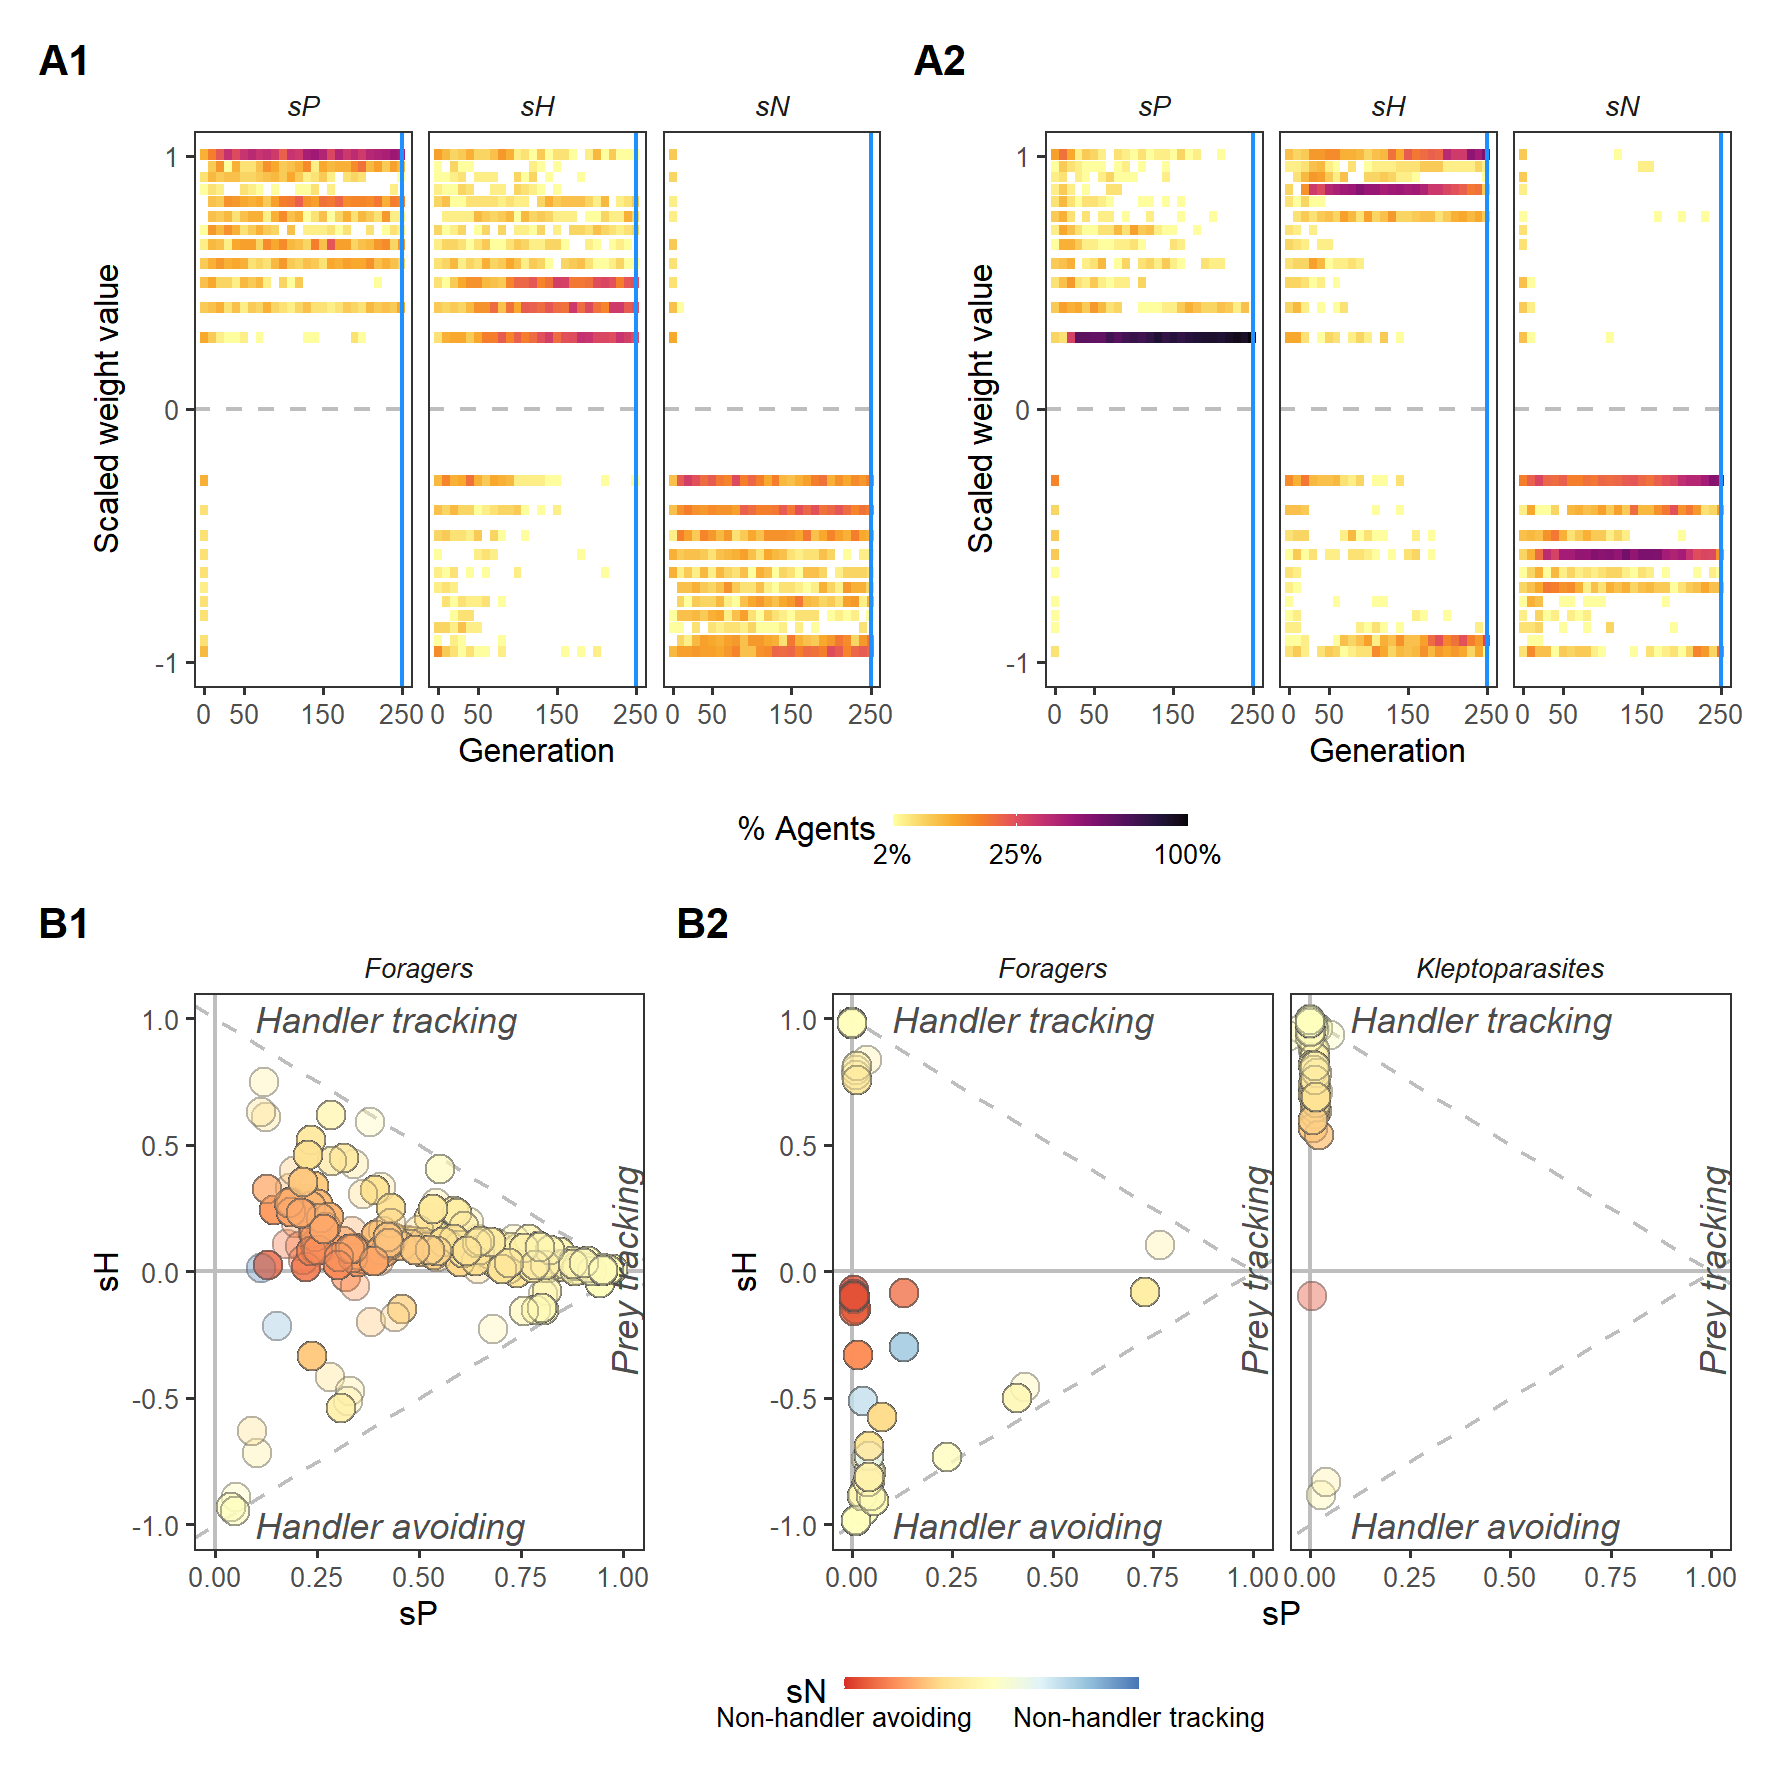
\includegraphics[width=0.90\textwidth]{figures/patternprocess/fig_01.png}
        \caption{
            \textbf{Evolutionary equilibrium and functional variation in movement rules in a spatially explicit, individual-based model of animal movement.}
            We find substantial polymorphism in movement rules in both scenarios of our spatially explicit, individual-based model of the joint evolution of animal movement and competition strategies.
            Agents in both \textbf{(A1)} scenario 1 (exploitation competition only), and in \textbf{(A2)} scenario 2 (fixed, individual competition strategies), evolve multiple, distinct, co-existing values of each of the weights controlling movement rules in the forms of preferences for each cue: $s_P$ (prey-items), $s_H$ (agents handling prey, `handlers'), and $s_N$ (idle agents, `non-handlers').
            The morphs persist across generations, indicating that they likely have equivalent foraging success, and hence, fitness outcomes.
            \textbf{(B1)} In the exploitation competition scenario, the evolved population (at G = 250; blue line in panels A1 and A2) has wide individual variation in their relative preferences for environmental cues (the scaled weights $s_P, s_H, s_N$).
            Most agents trade a preference for prey-items against either an avoidance of non-handlers (orange points), or a preference for handlers (yellow points with $s_H > 0.5$).
            \textbf{(B2)} In the fixed-strategy scenario 2, agents of the two competition strategies (foragers and kleptoparasites) have very different relative preferences for environmental cues.
            While foragers largely either avoid handlers (yellow points, $s_H < -0.5$), or avoid non-handlers (red points), most kleptoparasites prefer moving towards handlers, their direct resource.
            A small number of both foragers and kleptoparasites follow the movement rules of the opposite strategy; these likely represent a strategy mutation during reproduction.
            All panels show simulation runs with $r_{max}$ = 0.01, and show a single replicate for clarity.
        }
        \label{fig1}
    \end{figure}
    
    \begin{figure}[h!]
        \centering
        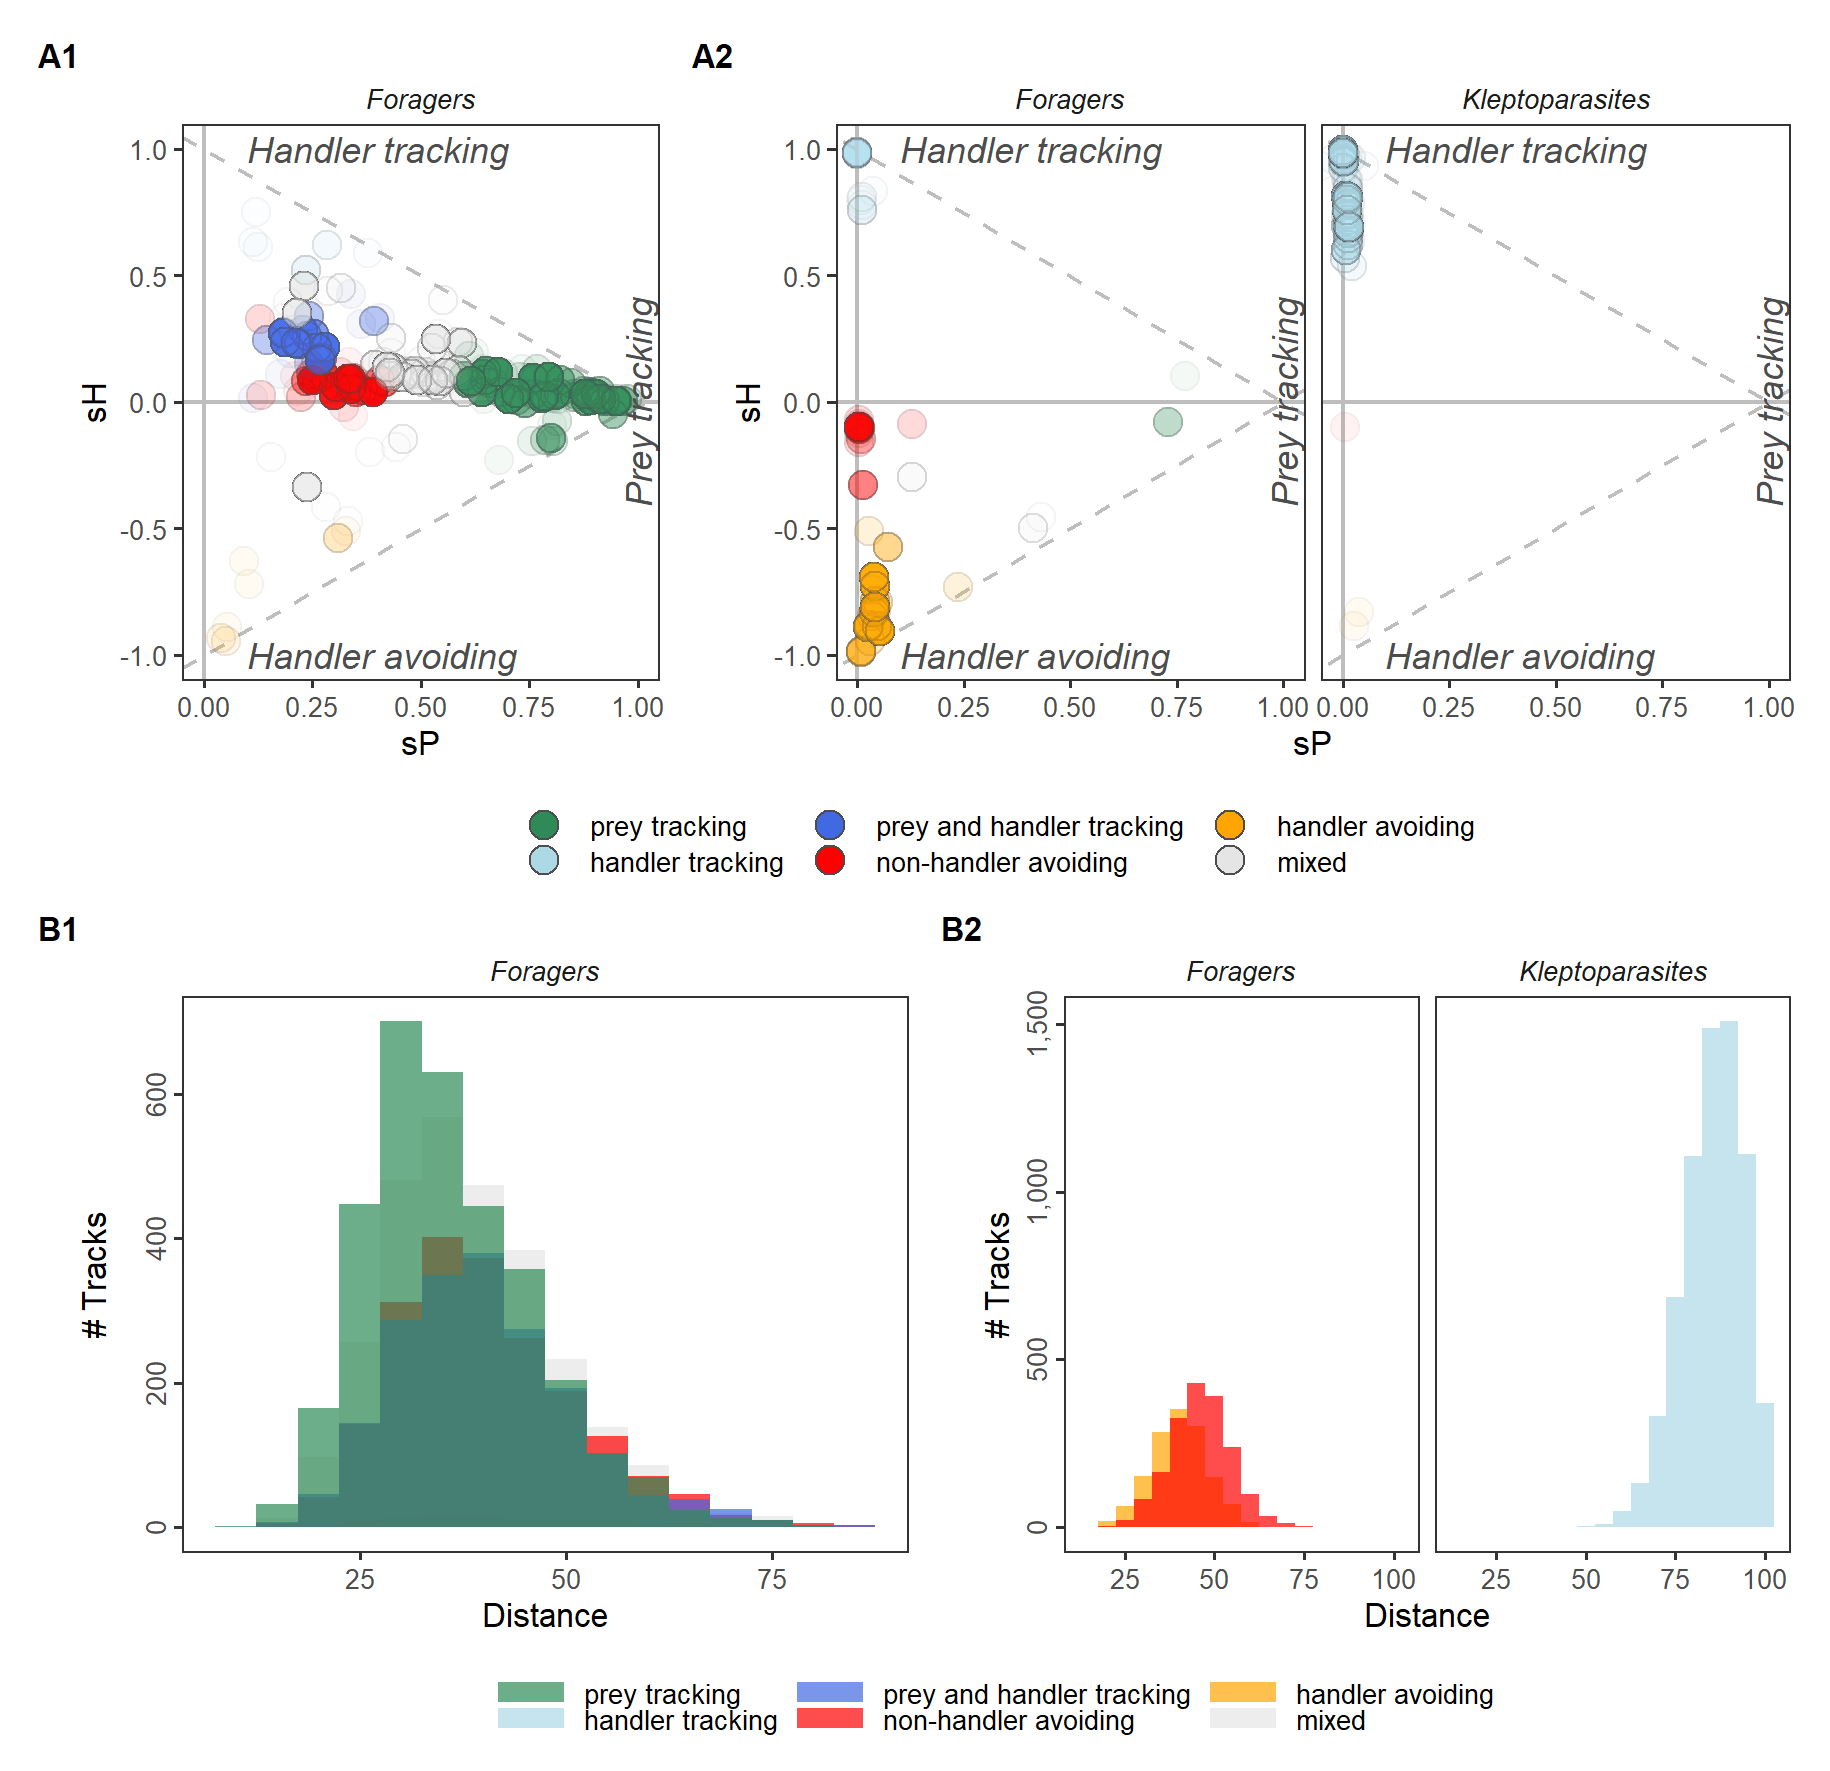
\includegraphics[width=0.90\textwidth]{figures/patternprocess/fig_02.png}
        \caption{
            \textbf{Movement types and competition strategies, and differences in movement paths.}
            We classified agents in both scenario 1 \textbf{(A1)} and scenario 2 \textbf{(A2)} into intuitive `movement types', based on their relative preferences for environmental cues (see Fig. 1 and Main Text). 
            We plotted them based on their weights for prey-items and handlers, adding a transparency to show the frequencies of the types.
            By this simple classification, agents in scenario 1 \textbf{(A1)} mostly track prey-items, or both prey-items and handlers, while avoiding non-handlers.
            Agents in the `mixed' strategy mostly track prey-items and avoid non-handlers.
            In scenario 2 \textbf{(A2)}, most foragers avoid other agents, either handlers or non-handlers; meanwhile, kleptoparasites, as expected, track their primary resource, handlers.
            Regardless of their movement type, agents in \textbf{(B1)} the exploitation scenario all move roughly the same distance in each interval.
            \textbf{(B2)} However, in the kleptoparasitism scenario, the competition strategies differ strongly, with kleptoparasites moving nearly twice as much as foragers.
            Despite moving according to quite different rules (avoid handlers, or avoid non-handlers), both types of foragers move nearly the same distance on average.
            While kleptoparasites' greater movement should be expected to lead to less time for handling prey, and hence lower intake, they save on this time by taking advantage of pre-handled items stolen from foragers.
            Panels A1 and A2 show 5,000 individuals from a single replicate of each scenario, while panels B1 and B2 show the mean movement distance of 100 agents over segments of 100 timesteps from all 10 replicates.
        }
        \label{fig2}
    \end{figure}
    
    \subsection*{Movement Cues, Competition Strategies, and Repeatability of Movement Distance}
    
    Our simulation's populations, at the eco-evolutionary equilibrium (G = 250) were comprised of individuals with a broad range of movement strategies (Fig. \ref{fig3}A).
    In \textbf{scenario 1}, a wider range of movement strategies were evolved on higher productivity landscapes ($r_{max}$ $\in$ 0.02, 0.03), than on lower productivity landscapes ($r_{max}$ = 0.01); the pure handler-tracking and handler avoiding strategies were seen only at at higher growth rates (Fig. \ref{fig3}A1).
    This suggests that on higher productivity landscapes, a wider range of movement types have equivalent fitness.
    The mechanism enabling this is the increased abundance of prey-items: as more agents find prey more easily and become handlers, the relative strength and frequency of the handler cue increases, and navigating using this social information alone becomes a viable movement strategy.
    
    The repeatability of movement distance is nearly five times as high on more productive landscapes ($r_{max}$ $\in$ 0.02, 0.03; repeatability $\approx$ 0.70), as on low productivity landscapes ($r_{max}$ = 0.01; repeatability $\approx$ 0.15; Fig. \ref{fig3}B1).
    This large difference may be because there are more movement types on high-productivity landscapes (Fig. \ref{fig3}A1), with subtle differences in distance moved among them.
    Yet, another plausible explanation is that on high productivity landscapes, there are simply more movement cues, in the form of prey-items and handlers.
    Since the movement types differ in how they process and respond to cues, movement on landscapes with more cues might better reveal subtle differences among the behavioural types.
    
    In \textbf{scenario 2}, increasing productivity also allows a wider range of forager, but not kleptoparasite, movement strategies (Fig. \ref{fig3}A2).
    At the index $r_{max}$ of 0.01, foragers are mostly agent avoiding, while kleptoparasites are handler tracking.
    However, with increasing growth rates, the frequency of kleptoparasites decreases, until, at $r_{max}$ = 0.03, kleptoparasites are extinct in nearly all simulation replicates.
    Thus, on high productivity landscapes, the scenario 2 population is functionally identical to the scenario 1 population, and all individuals follow a forager strategy.
    
    Repeatability analyses on the movement distances of scenario 2 populations is sensitive to how the differences in competition strategy are treated, but not to landscape productivity (Fig. \ref{fig3}B2). Specifically,
    \textit{(1)} When repeatability analysis ignores differences in competition strategy, our populations, comprised largely of handler and non-handler avoiding foragers, and handler tracking kleptoparasites, had repeatability scores $>$ 0.8 (Fig. \ref{fig3}B2a).
    This would suggest that nearly all the variance in movement distance not explained by the fixed effect of environmental productivity is due to between-individual differences (which we know to be primarily differences in competition strategy).\\
    %%
    \textit{(2)} When competition strategy is included as a fixed effect in repeatability analysis, repeatability scores drop substantially to $<$ 0.5 (Fig. \ref{fig3}B2b).
    This suggests that while competition strategies are important in explaining differences in movement distance, a substantial chunk of the unexplained variance is comprised of between-individual variance.\\ 
    %%
    \textit{(3)} Finally, in another plausible way of treating data when the existence of competition strategies is known, running separate repeatability analyses for foragers and kleptoparasites reveals very different repeatability scores for the two strategies (Fig. \ref{fig3}B2c).
    While foragers have repeatabilities betwen 0.0 and 0.75, depending on the growth rate, kleptoparasites have repeatabilities close to zero.
    
    There did not appear to be an effect of landscape productivity as in scenario 1.
    This may be because, in scenario 2, the presence of kleptoparasites (indeed, as the majority strategy) reduces prey-item extraction from the resource landscape.
    Consequently, all scenario 2 landscapes eventually resemble scenario 1 landscapes at $r_{max}$ = 0.03.
    We ran analyses only on growth rates of 0.01 and 0.02, as kleptoparasites rapidly go extinct early on in simulations with a growth rate of 0.03 (see Chapter~\ref{ch:kleptomove} for an explanation of the evolutionary dynamics).
    
    \begin{figure}[h!]
        \centering
        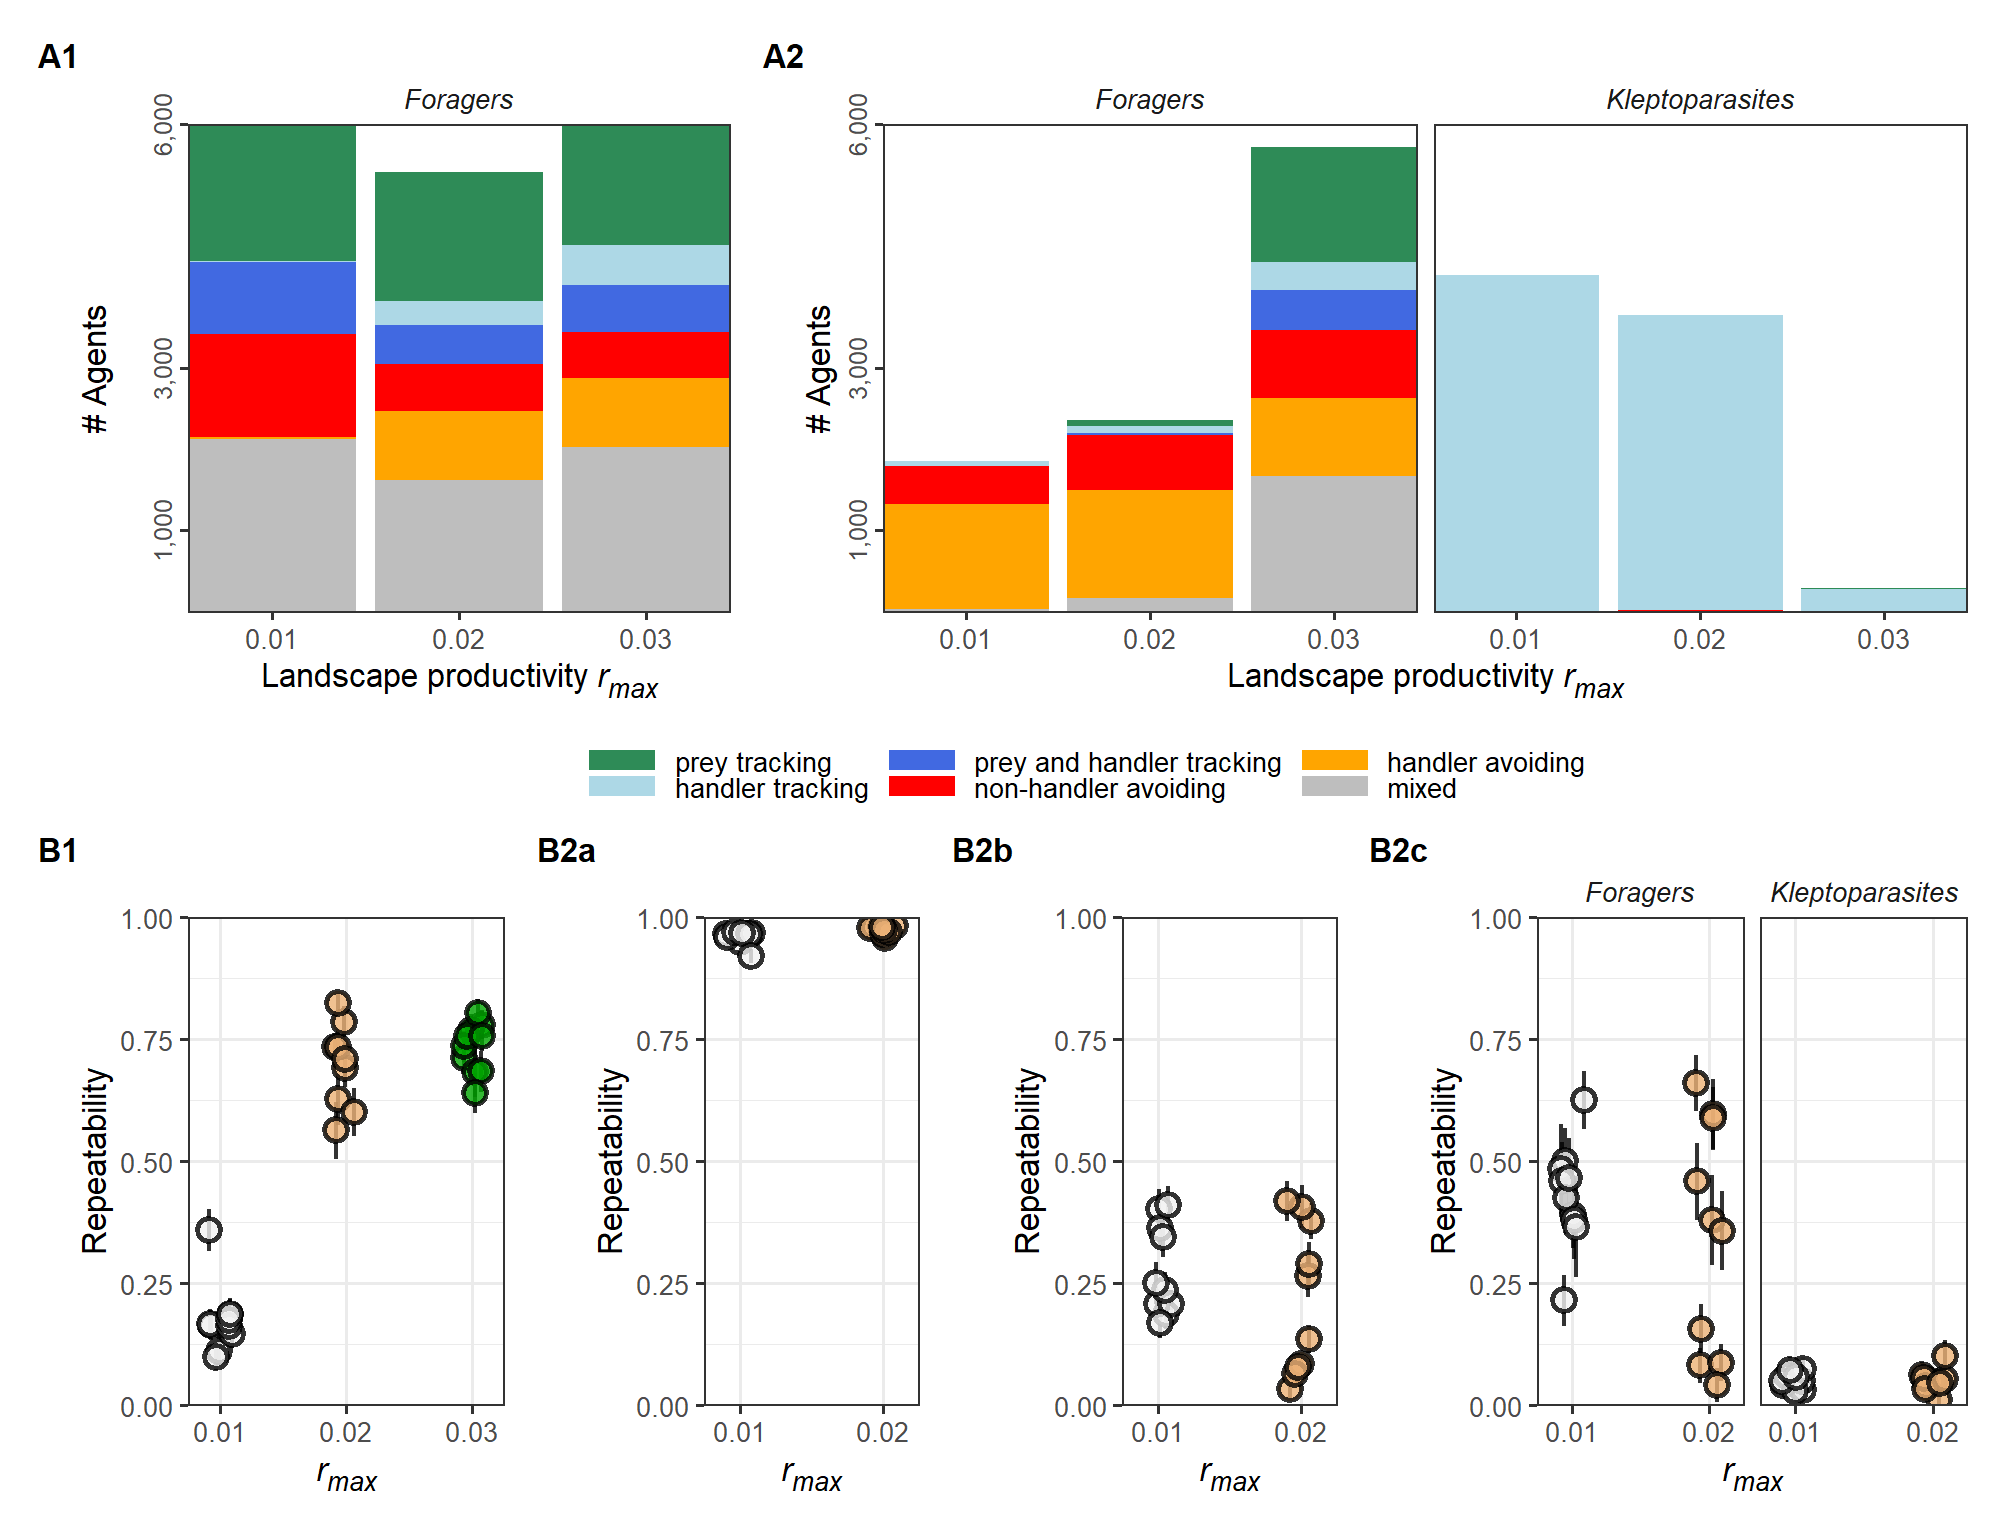
\includegraphics[width=1.0\textwidth]{figures/patternprocess/fig_03.png}
        \caption{
            \textbf{Frequency of movement types, competition strategies, and environmental cues, and consequences for repeatability analyses to detect individual differences in movement.}
            Increasing landscape productivity ($r_{max}$) beyond the index value of 0.01 leads to more prey-items on the landscape, and hence more available cues for movement decisions.
            In \textbf{(A1)} scenario 1, this leads to a change in the frequencies of movement types, with the persistence of handler-avoiding and pure handler-tracking types.
            In \textbf{(A2)} scenario 2, the frequencies of both movement types and competition types change with the increased availability of prey-items: at higher $r_{max}$ (0.03), foragers are both more common, and use more movement strategies, than at lower $r_{max}$ (0.01).
            The repeatability of movement distance is greater for scenario 1 populations on landscapes with higher $r_{max}$, and hence more available movement cues \textbf{(B1)}.
            This suggests that individual differences in movement decision-making mechanisms may be more readily detected when agents are actually able to process environmental cues using those mechanisms, rather than when agents move on relatively `clueless landscapes'.
            When agents' competitive strategy strongly influences their movement, as in scenario 2 \textbf{(B2 panels)}, repeatability analyses are strongly affected by how this difference is treated.
            \textbf{(B2a)} If differences in competitive strategies are not included in the model formulation, repeatability scores are consistently high ($>$ 0.9).
            \textbf{(B2b)} When agents' competitive strategy is included as a fixed effect, repeatability scores are substantially lower ($< 0.5$).
            Finally, \textbf{(B2c)}, repeatability models run separately for each of the competitive strategies would essentially reveal that competitive types with strong dimorphism (or clustering) in movement types (here, foragers) have a higher repeatability than competitive types with a monomorphic movement strategy (here, kleptoparasites).
            Panels A1 and A2 show frequencies pooled over 100 agents from 10 replicate simulations, with agent data exported at G = 200, 210, \ldots 249.
            Panels B1 and B2 used long-term movement paths from 100 agents in generation 250, over 10 replicates. B2 omits $r_{max}$ = 0.03, as kleptoparasites are often extinct.
        }
        \label{fig3}
    \end{figure}
    
    \subsection*{Individual Differences in Habitat Selection}
    
    We fit 6,000 step-selection functions to thinned movement data from 60 simulation runs, with 10 replicates for each $r_{max}$ value (0.01, 0.02, 0.03) and scenario (1 and 2).
    In \textbf{scenario 1}, all agents forage and have a substantial preference for moving towards prey-items.
    Consequently, the estimated coefficients of their apparent selection for cell productivity $r$ are all positive, with no differences among the movement strategies (Fig. \ref{fig4}A1, B1).
    On the other hand, in \textbf{scenario 2}, the dramatic difference in competition strategies is reflected in the estimated coefficients of apparent selection for cell $r$; foragers have substantially lower (and even negative) selection for $r$ than kleptoparasites (Fig. \ref{fig4}A2).
    However, there is little difference between foragers moving mostly to avoid handlers or to avoid non-handlers (Fig. \ref{fig4}B2).
    %%
    As landscape productivity increases, scenario 2 populations, but not scenario 1 agents, show a shift in their selection for cell $r$.
    At higher growth rates ($r$ = 0.02), scenario 2 populations --- still comprised of about equal proportions of foragers and kelptoparasites (see Fig. \ref{fig3}) --- show substantially more overlap between the two strategies' selection for $r$ (Fig. \ref{fig4}A2).
    This is carried over as an overlap between the three main movement types (Fig. \ref{fig4}B2).
    At the highest growth rates, scenario 1 and scenario 2 populations are essentially identical, and the few kleptoparasites remaining in scenario 2 apparently select for $r$ similar to foragers.
    Overall, applying step-selection analysis to our model output suggests that differences between competition strategies, when associated with different movement types, could be revealed under certain conditions from animal movement paths.
    
    \begin{figure}[h!]
        \centering
        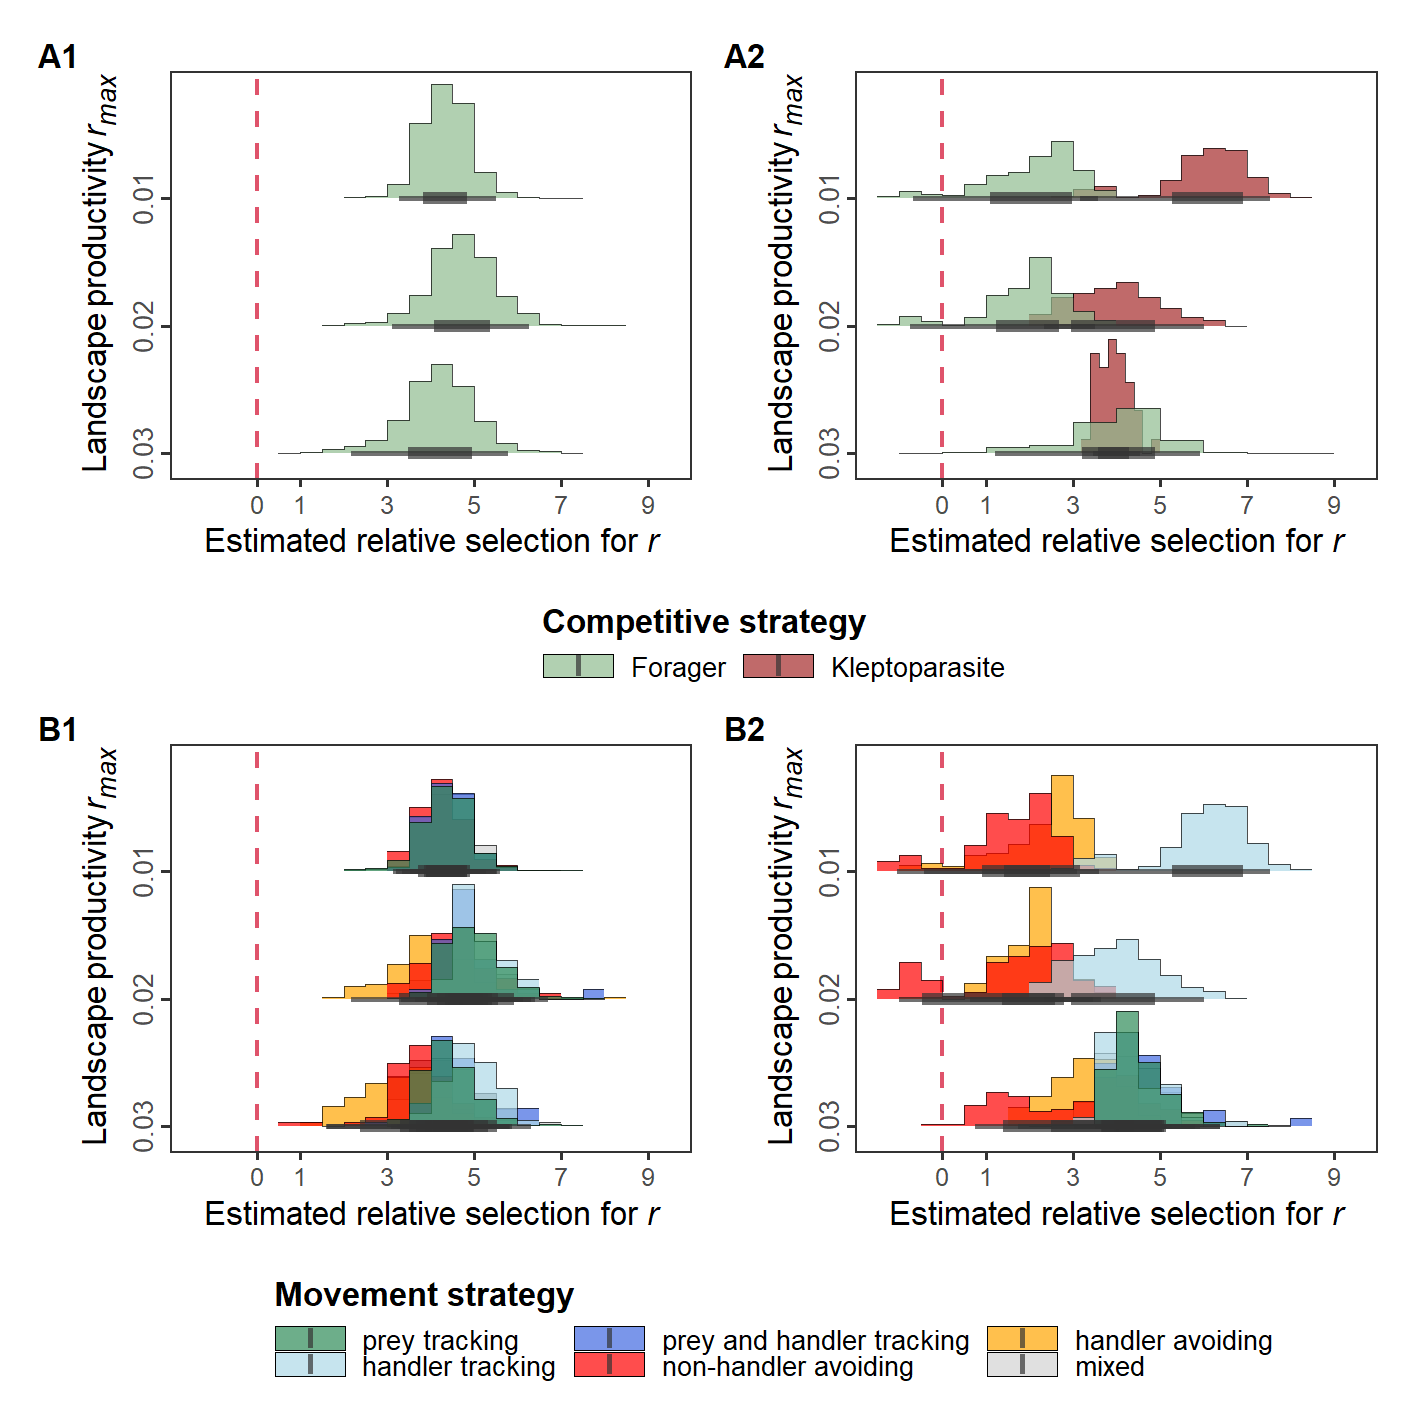
\includegraphics[width=0.90\textwidth]{figures/patternprocess/fig_04.png}
        \caption{
            \textbf{Movement types and competition strategies revealed in step-selection analyses.}
            Applying step-selection analysis to long-term movement paths from \textbf{(A1)} scenario 1, and \textbf{(A2)} scenario 2 reveals strong differences in apparent selection for landscape productivity between competition strategies ($r_{max}$ = 0.01).
            In \textbf{(B1)} scenario 1 and \textbf{(B2)} scenario 2, the apparent selection strengths for productivity $r$ of foragers of different movement types overlaps.
            Handler-tracking kleptoparasites in scenario 2, too, have apparent selection strengths for $r$ that overlap with those of some foragers, but which are substantially higher than those of most foragers, which avoid both handlers and non-handlers. 
            These essentially opposing movement strategies are picked up as differences in selection for $r$.
            Kleptoparasites track handlers, and the probability of a forager finding prey and handling are higher at the centres of resource peaks, i.e, cells with high $r$.
            Conversely, foragers avoid other agents, and since high-productivity cells are more likely to have agents, they apparently select \textit{against} high productivity cells.
            All panels show selection coefficients from 100 agents' long-term movement paths at G = 250, from 10 replicates of each simulation; only coefficients with $p \leq$ 0.05 are shown.
        }
        \label{fig4}
    \end{figure}
    
    \section*{Lessons for Data Analysis from the Performance of Statistical Methods on Simulated Data}
    
    % % Detecting Individual Consistency from Agent Paths
    
    We used an evolutionary individual-based model of animal movement decision-making under two scenarios of foraging competition (\textit{Kleptomove}; as described here and in Chapter~\ref{ch:kleptomove}), to investigate what we can learn about individual-differences by applying statistical analyses to animal movement data.
    % %%
    % We showed that the model, as expected, reached an ecological equilibrium in mean per-capita intake, as well as the mean per-capita distance moved.
    Our evolved agent populations showed substantial between-individual differences in their relative preferences for environmental cues (`movement types'; \citealt{getz2015}): when presented with the same cues, agents could make substantially different decisions about where to move.
    %%
    We showed that despite very different relative differences among the movement types for environmental cues, the types did not consistently differ in their movement distance.
    However, in our scenario 2, in which individuals had a fixed competition strategy (forager or kleptoparasite), kleptoparasites moved much more than foragers.
    %%
    With few between-type differences in movement distance, the repeatability of movement distance was low in scenario 1 at low growth rates, but increased substantially at higher growth rates.
    In scenario 2, not accounting for differences in competition strategy led to repeatability scores $\approx$ 1.0, but correcting for these differences led to lower repeatability scores.
    %%
    Finally, applying step-selection analysis to estimate agents' apparent selection for landscape productivity showed no differences among movement types in scenario 1, but revealed clear differences between competition strategies (and their correlated movement types) in scenario 2.
    %%
    % Our application of relatively simple analyses to a model with highly dynamic agent distributions,arising from simple movement rules and foraging mechanisms, emphasise the challenge in relating animals' behavioural mechanisms to the movement paths that are their outcomes.
    
    \subsection*{Variation Among Movement Types and Competition Strategies}
    
    The co-existence of multiple movement types across multiple generations of scenario 1 suggests that multiple alternative movement rules are equally good for navigating our fluctuating resource and social landscapes \citep[see also][]{getz2015,netz2021}.
    That movement types travel roughly the same distances is not surprising, as they must spend the same time handling, and gaining intake, to have equivalent fitness.
    In scenario 2, there are essentially only two viable movement types that are strongly correlated with competition strategies at low growth rates ($r_{max}$ = 0.01).
    Here, the handler-tracking kleptoparasites move more because their primary resource, handlers, are scarce; conversely, foragers move less, as prey-items are abundant.
    Yet both strategies have equivalent fitness because kleptoparasites make up for lost time by having to handle stolen prey-items for a shorter duration.
    We suggest that for movement types to differ in their path metrics (e.g. distance, or speed; see \citealt{abrahms2017}), between-individual variation and within-individual consistency along a further axis of behaviour that equalises fitness between the types is likely necessary.
    
    \subsection*{Repeatability Analysis}
    
    Repeatability analysis of the scenario 1 movement paths showed that populations evolved on higher productivity landscapes had significantly higher repeatability scores.
    The major difference between lower ($r_{max}$ = 0.01) and higher productivity landscapes ($r_{max}$ = 0.03) is that the latter have many more prey-items per cell.
    While agents on low growth rate landscapes often encounter areas with few or no movement cues (`clueless regions'; \citealt{perkins1992}), this is much more rarely the case on high productivity landscapes.
    Since our agents' decision-making mechanisms --- in common with animal cognitive systems --- require environmental cues to make movement decisions, between-individual differences in movement are more readily detected on landscapes with more movement cues \citep[see][]{carter2013a}.
    Our result might suggest that populations with different movement types transplanted between information-poor and information-rich landscapes would show a marked increase in behavioural consistency.
    We caution against this interpretation, as our populations have \textit{evolved}, rather than simply been tested on, landscapes across a productivity gradient.
    On high productivity landscapes, a wider range of movement types is evolved, highlighting how measures such as repeatability are linked to the evolutionary trajectory of populations.
    
    Using scenario 2, we illustrated three different ways of implementing repeatability analysis for a population with correlated differences in movement type and competition strategy.
    When differences in competition strategy were ignored, repeatability scores were close to 1.0, as the variance in movement distance due to competition strategy was picked up as between-individual variance instead.
    Adding competition strategy as a fixed effect to the analysis resulted in lower repeatability values; this was expected, as differences among competition strategies explain the bulk of the variance.
    Finally, performing separate repeatability analyses for foragers and kleptoparasites yielded very low repeatability scores for kleptoparasites, which foragers were still quite repeatable.
    This last result is potentially because kleptoparasites are solidly monomorphic in their movement type, while foragers may be either handler- or non-handler-avoiding, and this difference in decision-making mechanism could result in subtle differences in movement metrics.
    Overall, we suggest that extremely high repeatability scores might indicate that an important source of variation is not being taken into account, and should be sought for.
    Multivariate methods can help identify within-individual behavioural co-variation in movement metrics, such as distance and displacement \citep{hertel2019,hertel2021}.
    This approach could help reveal strong associations between movement types and competition strategies, as in our model, or responsiveness to social cues \citep{strandburg-peshkin2015}.
    Identifying such behaviours from animal movement data is likely to require very high-resolution tracking and associated computational methods (Nathan et al. \textit{in prep.}).
    
    \subsection*{Individual Differences in Habitat Selection}
    
    In a novel application of step-selection analysis to the study of individual differences, we showed that agents of different competition strategies (scenario 2), but not of different movement types (both scenarios 1 and 2), had diverging selection for environmental conditions.
    An important reminder is that our model's agents cannot actually detect cell productivity $r$, and therefore the preference for $r$ values is more correctly termed apparent selection.
    This situation parallels empirical analysis of animal tracking data, in which researchers commonly use long-term indices of environmental conditions (e.g. NDVI; \citealt{pettorelli2011}) to approximate the ephemeral movement cues actually encountered and acted upon by individuals.
    Nonetheless, strong between-individual differences (here, in competition strategy) are likely to be reflected in animals' apparent selection for environmental conditions.
    In our model, the difference in apparent selection arises from the distribution of movement cues relative to cell growth $r$.
    Handler-tracking kleptoparasites have a higher selection for $r$ because high-$r$ cells are more likely to have handlers, since foragers are more likely to find prey-items there and begin handling.
    On the other hand, agent-avoiding foragers have a lower selection for $r$ as they avoid resource peaks, which are more likely to have more agents.
    Some foragers will always be found on high-$r$ cells, as even a forager moving across the landscape at random (which they do not) is more likely to stop and begin handling on a high-$r$ cell than a cell at the periphery of a resource peak.
    
    \subsection*{Individual-based Models as a Check on Statistical Methods}
    
    Individual-based models are not new in movement ecology, and are increasingly used and prescribed to better understand animal movement \citep[see a review in][]{deangelis2019}.
    Such models have been used to illustrate the importance of animal movement to phenomena such as disease outbreaks \citep{white2018}, and sympatric speciation \citep{getz2015}, while also showing how individual differences in animal movement strategies can have downstream effects on population-level phenomena such as habitat-selection and social interactions \citep{spiegel2017,spiegel2016a}.
    There is also a rich tradition of individual-based models being used to assess the performance of methods intended for use on empirical tracking data.
    For example, \citealt{gurarie2016}, \citealt{michelot2016}, and \citealt{patin2020a} simulated the paths of individuals with different behavioural modes to test the performance of tools to detect behavioural change-points, where the animal switches from one movement mode to another.
    However, very few individual-based models that are used as checks on statistical methods actually model the fine-scale decisions --- comprising comparisons among, and eventual selection of --- steps that comprise animal movement \citep[but see recently][]{vissat2021}.
    This is at least partially because few statistical methods seek to estimate animal movement preferences, and by implication, animal cognitive processes, at such fine scales.
    Step-selection analysis has the potential to be among these methods, as it directly links what animals actually perceive, to where they go \citep[see recently][]{aben2021}.
    This allows a fine-scale comparison between selected and alternative steps, which, at certain scales, may functionally approximate individuals' cognitive processes, at least in terms of preference or avoidance.
    
    Our model and other mechanistic individual-based models that follow similar principles \citep{getz2015,getz2016,netz2021}, allow for the implementation of different movement decision-making mechanisms at very fine scales, in biologically plausible ways.
    Our agents' movement decisions integrate locally available cues to make adaptive movement decisions, just as real animals are expected to do \citep{nathan2008a}.
    While our agent responses are linear, they can in principle be much more complex, including convoluted relationships between the environmental cues, as well as separate weights for each cue combination.
    Coupled with the ability to know the state of the environment, and of each agent, at any point in the simulation, we believe this and other similar models are suitable for the testing of a range of empirical methods.
    For example, a better test of whether step-selection analysis can determine agent preferences for environmental cues, and individual differences therein, could involve the dynamic logging of selected and alternative steps, as well as the environmental covariates (prey-items and competitors) at those steps, in order to compare between them at fine scales.
    Such logging would immediately reveal that often, agents have either very few direct local cues, or very few differences between conditions at alternative and selected steps, on which to base movement decisions at fine timescales \cite[relatively clueless regions, per][]{perkins1992}.
    This highlights a potential challenge to such analyses from the ever increasing resolution of animal tracking and environmental monitoring data; for example, how should step-selection analysis be adapted to account for high spatial- and temporal-autocorrelation in animals' environments, while still taking advantage of high sampling frequencies.
    
    \section*{Conclusion}
    
    The analysis of our model's agent movement paths using contemporary statistical tools from movement ecology showed that it is often challenging to infer animals' decision-making processes, or even relative differences among individuals, from tracking data alone.
    First, when seeking to assess individual consistency and between-individual differences from animal tracking data, it is key to include predictors that have a mechanistic relationship with the behavioural response being studied.
    For species that are only poorly known, or difficult to study in captivity, this requires first collecting substantial knowledge on natural history and behavioural biology.
    Researchers could potentially apply a model selection approach \citep{burnham2011}, to determine which fixed effects are best suited to their study species.
    Second, uncovering individual behavioural tendencies in captivity may not be sufficient to describe animal movement in natural environments, which is likely to be affected by fine-scale fluctuations in resources, as well as the social environment.
    Finally, attempting to recover animals' movement preferences at fine scales is a challenging task.
    In part, this is due to a mismatch of scales: empirical researchers are rarely able to study fine-scale movement decisions, because suitably fine-scale data on the environmental cues that go into these decisions are not available.
    While increasingly high-resolution animal tracking is becoming more common, there would need to be a concurrent increase in the resolution of environmental monitoring \textit{from the animal's point of view}.
    The availability of such data sources would make the development of statistical tools that account for particular issues --- such as spatio-temporal autocorrelation --- a priority in movement ecology.
    Individual-based models, in which simple mechanisms can give rise to substantial complexity in animal movement and population distributions, could be very useful as test-beds to investigate whether current and upcoming tools are truly capable of parsing patterns to recover the underlying processes.
    
    { \begin{center} \barfont{-.-} \end{center} }

    % \section*{Data and Code Availability}
    
    % The simulation code for the \textit{Kleptomove} model is on Zenodo as \citealt[(zenodo.org/record/4905476)]{netz2022a}, and on Github: github.com/pratikunterwegs/Kleptomove.
    % %
    % Simulation data are available from DataverseNL as a draft: \textbf{UPDATE WITH DRAFT DATA}.
    % Data will be at this persistent link after publication: \textbf{UPDATE WITH PERSISTENT DOI}.
    % Data analysis code is on Github: github.com/pratikunterwegs/pattern-process.
    
    % \section*{Acknowledgments}
    
    % The authors thank Christoph Netz and Hanno Hildenbrandt for contributing extensively to the coding of the simulation model \textit{Kleptomove};
    % Jakob Gismann and other members of the Modelling Adaptive Response Mechanisms Group at the University of Groningen for helpful discussions on the manuscript.
    % F.J.W. acknowledges funding from the European Research Council (ERC Advanced Grant No. 789240).
    % P.R.G was supported by an Adaptive Life Programme grant made possible by the Groningen Institute for Evolutionary Life Sciences (GELIFES).

%     \newrefcontext[sorting=nyt]
%     \section*{Literature Cited}
%     \printbibliography[title=Literature~Cited,heading=none]
% \end{refsection}


% \include{Chapters/Chapter02}
%\addtocontents{toc}{\protect\clearpage} % <--- just debug stuff, ignore
% \include{Chapters/Chapter03}
%\include{multiToC} % <--- just debug stuff, ignore for your documents

\cleardoublepage 
\phantomsection
% \addtocontents{toc}{\protect\vspace{\beforebibskip}}%
% \addcontentsline{toc}{chapter}{\tocEntry{\color{black}\scshape\bfseries{General~Discussion: Linking the Ecology and Evolution of Animal Movement with Mechanistic, Individual Based Models}}}%
\chapter{{\color{gray}General~Discussion}\\Linking the Ecology and Evolution of Animal Movement with Mechanistic, Individual Based Models}
% \chaptermark{Linking the Ecology and Evolution of Animal Movement with Mechanistic, Individual Based Models}

{{Pratik R. Gupte}}

\section*{Recapitulation of this thesis}

\section*{Case studies: why movement is key to ecological patterns}

\section*{Why include evolution in animal movement studies}

\subsection*{Importance of the individual-centric view}

\subsection*{How evolved movement strategies are different from random movement}

\subsection*{Evolution of complex traits can be very rapid}

\section*{Conceptual ingredients of eco-evolutionary individual-based models}

\section*{Practical aspects of implementing eco-evolutionary individual-based models}

\section*{Relating individual-based models with empirical approaches in movement ecology}

\section*{Conclusion: Where are we now, and where is focus necessary?}


\cleardoublepage %********************************************************************
% Bibliography
%*******************************************************
% work-around to have small caps also here in the headline
% https://tex.stackexchange.com/questions/188126/wrong-header-in-bibliography-classicthesis
% Thanks to Enrico Gregorio
% \defbibheading{bibintoc}[\bibname]{%
%   \phantomsection
%   \manualmark
%   \markboth{\spacedlowsmallcaps{#1}}{\spacedlowsmallcaps{#1}}%
%   \addtocontents{toc}{\protect\vspace{\beforebibskip}}%
%   \addcontentsline{toc}{chapter}{\tocEntry{#1}}%
%   \chapter*{#1}%
% }
% \printbibliography[heading=bibintoc]

% BIBLIOGRAPHY
\begingroup
  \newrefcontext[sorting=nyt]
  \addtocontents{toc}{\protect\vspace{\beforebibskip}}%
  \addchap{Literature Cited in this Thesis}
  \markboth{\color{gray}\small\scshape\rmfamily{Bibliography}}{\color{gray}\small\scshape\rmfamily{Bibliography}}
  \printbibliography[heading=none]
\endgroup

% Old version, will be removed later
% work-around to have small caps also here in the headline
%\manualmark
%\markboth{\spacedlowsmallcaps{\bibname}}{\spacedlowsmallcaps{\bibname}} % work-around to have small caps also
%\phantomsection
%\refstepcounter{dummy}
%\addtocontents{toc}{\protect\vspace{\beforebibskip}} % to have the bib a bit from the rest in the toc
%\addcontentsline{toc}{chapter}{\tocEntry{\bibname}}
%\label{app:bibliography}
%\printbibliography


\clearpage %*******************************************************
% Publications
%*******************************************************
% \pdfbookmark[1]{Acknowledgments}{acknowledgments}
% \phantomsection
% \addtocontents{toc}{\protect\vspace{\beforebibskip}}%
% \addcontentsline{toc}{chapter}{\tocEntry{Publications Related to this Thesis}}%
\addchap{About the Author}\label{ch:pubs}
\chaptermark{About the Author}

\begingroup

Pratik R. Gupte was born in India in 1993.
After schooling in Hyderabad and an undergraduate degree in zoology from St. Xavier's College, Mumbai in 2014, he worked on field projects in southern India, Ladakh, and in South Africa.
In 2017 he received a master's degree from the University of Kiel, as part of the International Master's in Applied Ecology, a programme spread over France, Portugal, Germany, and Ecuador.
His master's thesis on families of wintering Arctic geese saw fieldwork in the Russian Arctic and the Netherlands.
In 2018, he began his PhD in Franjo Weissing's lab at the University of Groningen.
Pratik is broadly interested in the spatial ecology of animals, especially birds.
Recognising that the current model of academic science is unsustainable, he left the academic career track, and is now a research software engineer at the London School of Hygiene and Tropical Medicine, where he develops epidemiological models to inform policy responses to disease outbreaks.

\let\clearpage\relax
\let\cleardoublepage\relax
\let\cleardoublepage\relax

\begin{refsection}
    \small
    \nocite{gupte2021a,gupte2022c,gupte2022d,thaker2019,nathan2022,netz2022,ramesh2022,
        bijleveld2021,rimbach2022un,gupte2019} % is local to to the enclosing refsection
    \printbibliography[title=Author Publications]
\end{refsection}

\begin{refsection}
    \small
    \nocite{gupte2022,gupte2022e,gupte2022b,gupte2021b,gupte2020a,gupte2022f,netz2021b,netz2022a,netz2021b} % is local to to the enclosing refsection
    \printbibliography[title=Data and Code]
\end{refsection}

\endgroup

{ \begin{center} \barfont{-.-} \end{center} }

% \emph{Attention}: This requires a separate run of \texttt{bibtex} for your \texttt{refsection}, \eg, \texttt{ClassicThesis1-blx} for this file. You might also use \texttt{biber} as the backend for \texttt{biblatex}. See also \url{http://tex.stackexchange.com/questions/128196/problem-with-refsection}.


% \clearpage %*******************************************************
% Acknowledgments
%*******************************************************
% \pdfbookmark[1]{Acknowledgments}{acknowledgments}
\addchap{Reflections and Acknowledgments}\label{ch:ack}
% \chaptermark{Reflections and Acknowledgments}

% \begin{flushright}{\slshape
%     We have seen that computer programming is an art, \\
%     because it applies accumulated knowledge to the world, \\
%     because it requires skill and ingenuity, and especially \\
%     because it produces objects of beauty.} \\ \medskip
%     --- \defcitealias{knuth:1974}{Donald E. Knuth}\citetalias{knuth:1974} \citep{knuth:1974}
% \end{flushright}

\bigskip

\begingroup
\let\clearpage\relax
\let\cleardoublepage\relax
\let\cleardoublepage\relax

Having read many thesis ``Acknowledgments'', the general pattern is to express a great sense of achievement, with thanks to family, friends, and supervisors.
Instead, I want to reflect on the PhD and the past four years generally.
People tend to rationalise their choices in hindsight, and this section may be no different.

It was probably not a good idea for me to have undertaken this PhD, perhaps a PhD at all.
I don't have the unbounded curiosity or creativity that defines `good' academics.
Rather, I should probably have been an engineer --- I enjoy getting things done.
I suppose I must say that I didn't know any better than to start a PhD, and that I wanted to conform socially with my friends, many of whom were starting PhDs, and that it did at the time represent a great deal of stability at a relatively high income.

I'm now convinced that I did not choose my PhD situation wisely.
Both of my `main' supervisors were in a state which I now recognise is not at all easy for their first few PhD students --- they were starting, or re-starting, their labs.
While one issue with a new lab is the relative inexperience of the supervisor, the more important one is actually the lack of a lab culture.
This includes accumulated wisdom that is invaluable to those receiving it; for those first uncovering it, it is often dearly won.
This is exactly the situation in which I found myself from beginning to end --- there was nobody around to show me the ropes, because there was nobody ahead of me to know them.

My lab also suffered --- and still does --- from being much too large. 
There were (and are) too many lines of research, all of them quite different.
I would have appreciated a smaller, more focused lab.
It was also very frustrating that my supervisors were pulling in wildly different directions (in a meeting, they once called each others' work ``irrelevant'').
There was a constant tension between where I was based (in a theoretical lab), and what I was good at (working with empirical data).

Then the pandemic happened.
In 2020, being securely employed for two more years was a huge advantage.
For that, I was, and remain, grateful; without the pandemic, though, I would have quit my PhD midway.

\paragraph*{Supervisors}

I've thought a great deal about whether to thank my supervisors --- this should already make it clear that I was less than pleased with how they operated.

First, I bear Ton Groothuis --- who was initially supposed to have been my second promotor, as well as Theunis, no ill will.
They were largely absent for most of my PhD, and I also did not seek them out.
I'm glad Ton did not insist that I should align with his interests, which don't overlap with mine at all.
However, I regret not working with Theunis because I think I would have found some satisfaction in the kind of work he does.

Second, I think Allert shouldn't be supervising anybody, let alone PhD students.
He was unreliable across contexts, quick to agree with senior people he respected, quick to rubbish ideas he didn't, and I never sensed a `big picture' in his work.
I felt he tried to hold me back to protect his less able student, and took advantage of my skills and generally helpful nature.
He appears in this thesis simply because it was considered too time-consuming to remove him.

In contrast, Ran Nathan joined my promotors' committee very late --- just a few days before I turned in my thesis.
The idea of including him grew on me slowly, and was cemented when I began collaborating with him directly in the summer of 2021, to replace the projects I lost when I stopped working with Allert.
I found Ran, even when not my supervisor, to be supportive and helpful, with exactly the sort of `big picture' view I had been lacking in relation to tracking data.

Finally \ldots

\paragraph*{Collaborators}

I had the good fortune to have worked with two ambitious and driven people.

Vijay Ramesh, then at Columbia University (now at Cornell) reached out to ask whether I would help him with some spatial data in late 2018.
I joined him in a 6-month project that ran for three and a half years --- see Chapter~\ref{ch:hillybirds}.
I used this project as a testbed for new techniques --- using Python for some computations, and ideas --- spatial thinning using a network approach, that caught my interest.

Greg Albery is among my most recent collaborators, and someone whose work I've held in high regard for a while.
In early 2021, Greg tried to recruit me to his supervisor's lab at Georgetown (he tried again in early 2022).
I was sounded out to work on building social networks from animal movement data, with a potential expansion into examining disease transmission.
This gave me the idea for Chapter~\ref{ch:pathomove}, during which I learned the movement and disease modelling that landed me my current job.

I look forward to working with both Vijay and Greg in the years to come.

I've had the help of many other collaborators at all levels in academia, who appear as authors on some of the chapters in this thesis, and on manuscripts yet to come: Orr Spiegel, Sivan Toledo, Yosef Kiat, Yoav Barton, Ulrike Schl{\"a}gel, Johannes Signer, Mark Adams, Rebecca Rimbach, Mridula Paul, Morgan Tingley, VV Robin, Ruth de Fries, and Amy Sweeny.

\paragraph*{TRES and Surrounds}

Joining TRES in mid-2018, I found a department that, pre-pandemic, was very similar to the Centre for Ecological Sciences I was coming from --- full of intelligent people, and most importantly, social.
I will freely admit to not finding the majority of the work in this department interesting, and that was a function of the diversity, or divergence, of topics among and within labs.
Yet the general gregariousness of the PhD students who were my colleagues more than made up for this.
I now think departments with better social than professional ties are probably healthier workplaces.

A number of people here 

I'm quite sure my life would be very different without Josh Lambert.
I would never have tried a number of things I now enjoy without Josh suggesting them, and often, accompanying me: squash, long-distance cycling, programming in Julia, considering the UK to live and work.
I also made a more serious change, of which Josh convinced me: to eventually leave the academic track.
I'm immensely pleased that I was able to find a cluster-hire at the London School of Hygiene and Tropical Medicine, through which we were both offered positions.
Josh is both very smart and grounded, and he's the first and last person I go to for advice --- I look forward to having him around.

\endgroup


% ********************************************************************
% Backmatter
%*******************************************************
\appendix
%\renewcommand{\thechapter}{\alph{chapter}}
% \clearpage
% \part{Appendix}
\cleardoublepage
%********************************************************************
% Other Stuff in the Back
%*******************************************************
%\clearpage%********************************************************************
% Bibliography
%*******************************************************
% work-around to have small caps also here in the headline
% https://tex.stackexchange.com/questions/188126/wrong-header-in-bibliography-classicthesis
% Thanks to Enrico Gregorio
% \defbibheading{bibintoc}[\bibname]{%
%   \phantomsection
%   \manualmark
%   \markboth{\spacedlowsmallcaps{#1}}{\spacedlowsmallcaps{#1}}%
%   \addtocontents{toc}{\protect\vspace{\beforebibskip}}%
%   \addcontentsline{toc}{chapter}{\tocEntry{#1}}%
%   \chapter*{#1}%
% }
% \printbibliography[heading=bibintoc]

% BIBLIOGRAPHY
\begingroup
  \newrefcontext[sorting=nyt]
  \addtocontents{toc}{\protect\vspace{\beforebibskip}}%
  \addchap{Literature Cited in this Thesis}
  \markboth{\color{gray}\small\scshape\rmfamily{Bibliography}}{\color{gray}\small\scshape\rmfamily{Bibliography}}
  \printbibliography[heading=none]
\endgroup

% Old version, will be removed later
% work-around to have small caps also here in the headline
%\manualmark
%\markboth{\spacedlowsmallcaps{\bibname}}{\spacedlowsmallcaps{\bibname}} % work-around to have small caps also
%\phantomsection
%\refstepcounter{dummy}
%\addtocontents{toc}{\protect\vspace{\beforebibskip}} % to have the bib a bit from the rest in the toc
%\addcontentsline{toc}{chapter}{\tocEntry{\bibname}}
%\label{app:bibliography}
%\printbibliography

% \clearpage%*******************************************************
% Declaration
%*******************************************************
\pdfbookmark[0]{Declaration}{declaration}
\chapter*{Declaration}
\thispagestyle{empty}
Put your declaration here.
\bigskip

\noindent\textit{\myLocation, \myTime}

\smallskip

\begin{flushright}
    \begin{tabular}{m{5cm}}
        \\ \hline
        \centering\myName \\
    \end{tabular}
\end{flushright}


% \clearpage%*******************************************************
% Publications
%*******************************************************
% \pdfbookmark[1]{Acknowledgments}{acknowledgments}
% \phantomsection
% \addtocontents{toc}{\protect\vspace{\beforebibskip}}%
% \addcontentsline{toc}{chapter}{\tocEntry{Publications Related to this Thesis}}%
\addchap{About the Author}\label{ch:pubs}
\chaptermark{About the Author}

\begingroup

Pratik R. Gupte was born in India in 1993.
After schooling in Hyderabad and an undergraduate degree in zoology from St. Xavier's College, Mumbai in 2014, he worked on field projects in southern India, Ladakh, and in South Africa.
In 2017 he received a master's degree from the University of Kiel, as part of the International Master's in Applied Ecology, a programme spread over France, Portugal, Germany, and Ecuador.
His master's thesis on families of wintering Arctic geese saw fieldwork in the Russian Arctic and the Netherlands.
In 2018, he began his PhD in Franjo Weissing's lab at the University of Groningen.
Pratik is broadly interested in the spatial ecology of animals, especially birds.
Recognising that the current model of academic science is unsustainable, he left the academic career track, and is now a research software engineer at the London School of Hygiene and Tropical Medicine, where he develops epidemiological models to inform policy responses to disease outbreaks.

\let\clearpage\relax
\let\cleardoublepage\relax
\let\cleardoublepage\relax

\begin{refsection}
    \small
    \nocite{gupte2021a,gupte2022c,gupte2022d,thaker2019,nathan2022,netz2022,ramesh2022,
        bijleveld2021,rimbach2022un,gupte2019} % is local to to the enclosing refsection
    \printbibliography[title=Author Publications]
\end{refsection}

\begin{refsection}
    \small
    \nocite{gupte2022,gupte2022e,gupte2022b,gupte2021b,gupte2020a,gupte2022f,netz2021b,netz2022a,netz2021b} % is local to to the enclosing refsection
    \printbibliography[title=Data and Code]
\end{refsection}

\endgroup

{ \begin{center} \barfont{-.-} \end{center} }

% \emph{Attention}: This requires a separate run of \texttt{bibtex} for your \texttt{refsection}, \eg, \texttt{ClassicThesis1-blx} for this file. You might also use \texttt{biber} as the backend for \texttt{biblatex}. See also \url{http://tex.stackexchange.com/questions/128196/problem-with-refsection}.

% \clearpage%*******************************************************
% Acknowledgments
%*******************************************************
% \pdfbookmark[1]{Acknowledgments}{acknowledgments}
\addchap{Reflections and Acknowledgments}\label{ch:ack}
% \chaptermark{Reflections and Acknowledgments}

% \begin{flushright}{\slshape
%     We have seen that computer programming is an art, \\
%     because it applies accumulated knowledge to the world, \\
%     because it requires skill and ingenuity, and especially \\
%     because it produces objects of beauty.} \\ \medskip
%     --- \defcitealias{knuth:1974}{Donald E. Knuth}\citetalias{knuth:1974} \citep{knuth:1974}
% \end{flushright}

\bigskip

\begingroup
\let\clearpage\relax
\let\cleardoublepage\relax
\let\cleardoublepage\relax

Having read many thesis ``Acknowledgments'', the general pattern is to express a great sense of achievement, with thanks to family, friends, and supervisors.
Instead, I want to reflect on the PhD and the past four years generally.
People tend to rationalise their choices in hindsight, and this section may be no different.

It was probably not a good idea for me to have undertaken this PhD, perhaps a PhD at all.
I don't have the unbounded curiosity or creativity that defines `good' academics.
Rather, I should probably have been an engineer --- I enjoy getting things done.
I suppose I must say that I didn't know any better than to start a PhD, and that I wanted to conform socially with my friends, many of whom were starting PhDs, and that it did at the time represent a great deal of stability at a relatively high income.

I'm now convinced that I did not choose my PhD situation wisely.
Both of my `main' supervisors were in a state which I now recognise is not at all easy for their first few PhD students --- they were starting, or re-starting, their labs.
While one issue with a new lab is the relative inexperience of the supervisor, the more important one is actually the lack of a lab culture.
This includes accumulated wisdom that is invaluable to those receiving it; for those first uncovering it, it is often dearly won.
This is exactly the situation in which I found myself from beginning to end --- there was nobody around to show me the ropes, because there was nobody ahead of me to know them.

My lab also suffered --- and still does --- from being much too large. 
There were (and are) too many lines of research, all of them quite different.
I would have appreciated a smaller, more focused lab.
It was also very frustrating that my supervisors were pulling in wildly different directions (in a meeting, they once called each others' work ``irrelevant'').
There was a constant tension between where I was based (in a theoretical lab), and what I was good at (working with empirical data).

Then the pandemic happened.
In 2020, being securely employed for two more years was a huge advantage.
For that, I was, and remain, grateful; without the pandemic, though, I would have quit my PhD midway.

\paragraph*{Supervisors}

I've thought a great deal about whether to thank my supervisors --- this should already make it clear that I was less than pleased with how they operated.

First, I bear Ton Groothuis --- who was initially supposed to have been my second promotor, as well as Theunis, no ill will.
They were largely absent for most of my PhD, and I also did not seek them out.
I'm glad Ton did not insist that I should align with his interests, which don't overlap with mine at all.
However, I regret not working with Theunis because I think I would have found some satisfaction in the kind of work he does.

Second, I think Allert shouldn't be supervising anybody, let alone PhD students.
He was unreliable across contexts, quick to agree with senior people he respected, quick to rubbish ideas he didn't, and I never sensed a `big picture' in his work.
I felt he tried to hold me back to protect his less able student, and took advantage of my skills and generally helpful nature.
He appears in this thesis simply because it was considered too time-consuming to remove him.

In contrast, Ran Nathan joined my promotors' committee very late --- just a few days before I turned in my thesis.
The idea of including him grew on me slowly, and was cemented when I began collaborating with him directly in the summer of 2021, to replace the projects I lost when I stopped working with Allert.
I found Ran, even when not my supervisor, to be supportive and helpful, with exactly the sort of `big picture' view I had been lacking in relation to tracking data.

Finally \ldots

\paragraph*{Collaborators}

I had the good fortune to have worked with two ambitious and driven people.

Vijay Ramesh, then at Columbia University (now at Cornell) reached out to ask whether I would help him with some spatial data in late 2018.
I joined him in a 6-month project that ran for three and a half years --- see Chapter~\ref{ch:hillybirds}.
I used this project as a testbed for new techniques --- using Python for some computations, and ideas --- spatial thinning using a network approach, that caught my interest.

Greg Albery is among my most recent collaborators, and someone whose work I've held in high regard for a while.
In early 2021, Greg tried to recruit me to his supervisor's lab at Georgetown (he tried again in early 2022).
I was sounded out to work on building social networks from animal movement data, with a potential expansion into examining disease transmission.
This gave me the idea for Chapter~\ref{ch:pathomove}, during which I learned the movement and disease modelling that landed me my current job.

I look forward to working with both Vijay and Greg in the years to come.

I've had the help of many other collaborators at all levels in academia, who appear as authors on some of the chapters in this thesis, and on manuscripts yet to come: Orr Spiegel, Sivan Toledo, Yosef Kiat, Yoav Barton, Ulrike Schl{\"a}gel, Johannes Signer, Mark Adams, Rebecca Rimbach, Mridula Paul, Morgan Tingley, VV Robin, Ruth de Fries, and Amy Sweeny.

\paragraph*{TRES and Surrounds}

Joining TRES in mid-2018, I found a department that, pre-pandemic, was very similar to the Centre for Ecological Sciences I was coming from --- full of intelligent people, and most importantly, social.
I will freely admit to not finding the majority of the work in this department interesting, and that was a function of the diversity, or divergence, of topics among and within labs.
Yet the general gregariousness of the PhD students who were my colleagues more than made up for this.
I now think departments with better social than professional ties are probably healthier workplaces.

A number of people here 

I'm quite sure my life would be very different without Josh Lambert.
I would never have tried a number of things I now enjoy without Josh suggesting them, and often, accompanying me: squash, long-distance cycling, programming in Julia, considering the UK to live and work.
I also made a more serious change, of which Josh convinced me: to eventually leave the academic track.
I'm immensely pleased that I was able to find a cluster-hire at the London School of Hygiene and Tropical Medicine, through which we were both offered positions.
Josh is both very smart and grounded, and he's the first and last person I go to for advice --- I look forward to having him around.

\endgroup

% ********************************************************************
% Game Over: Restore, Restart, or Quit?
%*******************************************************
\end{document}
% ********************************************************************
